\documentclass[english,fontsize=11pt,paper=a5,oneside]{scrbook}
%\usepackage{fourier}
%\usepackage{lmodern} % Improvement over cmtt
%\usepackage{cmbright}
\usepackage{sansmathfonts}

%\usepackage[utf8]{inputenc}
\usepackage[T1]{fontenc}
\usepackage{textcomp}
\renewcommand*\familydefault{\sfdefault}

\usepackage{booktabs}

\usepackage{xcolor}
\usepackage{graphicx}
\graphicspath{{images/}{../images/}}

\usepackage{mathtools}
\usepackage{amsmath, amssymb, amsthm}
\usepackage{bm}

\usepackage{units}

\usepackage{tikz}
\usepackage{pgfplots}
\usepackage{tikz-3dplot}
\pgfplotsset{compat=1.16}
\usepackage{wrapfig}
\usepackage{tcolorbox}
%\usepackage{todonotes}
% uncomment to tag only the referred equations (post-production)
\mathtoolsset{showonlyrefs,showmanualtags}

% comment before publication
%\usepackage{showlabels}

\usepackage[
    type={CC},
    modifier={by-nc-sa},
    version={4.0},
]{doclicense}

\usepackage{babel}
\usepackage{hyperref}
\hypersetup{
colorlinks,
linkcolor={blue!60!black},
citecolor={blue!60!black},
urlcolor={blue!60!black},
linktoc=page}
\DeclareTextCommandDefault{\textbullet}{\ensuremath{\bullet}}

\usepackage[numbers, sort]{natbib}
\setlength{\bibsep}{3pt}
\renewcommand{\bibfont}{\small}
\usepackage{doi}

\newcommand{\cC}{\mathcal{C}}
\newcommand{\cE}{\mathcal{E}}
\newcommand{\cL}{\mathcal{L}}
\newcommand{\cO}{\mathcal{O}}
\newcommand{\cH}{\mathcal{H}}
\newcommand{\cI}{\mathcal{I}}

%\newcommand{\C}{\mathbb{C}}
\newcommand{\N}{\mathbb{N}}
\newcommand{\Z}{\mathbb{Z}}
\newcommand{\R}{\mathbb{R}}
\newcommand{\T}{\mathbb{T}}
\newcommand{\bS}{\mathbb{S}}

\newcommand{\bx}{\bm{x}}
\newcommand{\bp}{\bm{p}}
\newcommand{\bv}{\bm{v}}

\newcommand{\lag}{\langle}
\newcommand{\rag}{\rangle}

\let\d\relax
\DeclareMathOperator{\d}{d}
\DeclareMathOperator{\D}{D}
\DeclareMathOperator{\Id}{Id}
\DeclareMathOperator{\diag}{diag}
\let\mod\relax
\DeclareMathOperator{\mod}{mod}
\DeclareMathOperator{\curl}{curl}
\DeclareMathOperator{\Vol}{Vol}

\newcommand{\pder}[2]{\frac{\partial{#1}}{\partial{#2}}}
\newcommand{\der}[2]{\frac{\d{#1}}{\d{#2}}}

\newtheorem{theorem}{Theorem}[chapter]
\newtheorem{proposition}[theorem]{Proposition}
\newtheorem{lemma}[theorem]{Lemma}
\newtheorem{corollary}[theorem]{Corollary}
\newtheorem{definition}{Definition}

\theoremstyle{definition}
\newtheorem{remarkx}{Remark}[chapter]
\newenvironment{remark}
  {\pushQED{\qed}\renewcommand{\qedsymbol}{$\lozenge$}\remarkx}
  {\popQED\endremarkx}
\newtheorem{examplex}{Example}[chapter]
\newenvironment{example}
  {\pushQED{\qed}\renewcommand{\qedsymbol}{$\lozenge$}\examplex}
  {\popQED\endexamplex}
\newtheorem{exercisex}{Exercise}[chapter]
\newenvironment{exercise}
  {\pushQED{\qed}\renewcommand{\qedsymbol}{$\maltese$}\exercisex}
  {\popQED\endexercisex}


\usepackage[toc,page]{appendix}
\usepackage{subfiles}

\title{Hamiltonian Mechanics}
\author{Marcello Seri\\
\small{Bernoulli Institute}\vspace{-.2cm}\\
\small{University of Groningen}\vspace{-.2cm}\\
\small\href{mailto:m.seri@rug.nl}{m.seri (at) rug.nl}
}
\date{}

% trick for bibliography in subfiles -- part 1
\def\biblio{\bibliographystyle{plainnat}\bibliography{../book}}

\usepackage{scrhack}
\begin{document}
% trick for bibliography in subfiles -- part 2
\def\biblio{}

\maketitle

\cleardoublepage

\thispagestyle{empty}
\null\vfill
\begin{center}
    Version 1.3.1\\
    \today
\end{center}
\vfill
\small{\doclicenseThis}

\cleardoublepage

\pagenumbering{roman}
\tableofcontents

\cleardoublepage

\pagenumbering{arabic}
\chapter*{Preface}

The literature on classical (or analytical, as it was called by Lagrange) mechanics is full of good material.
Different sources present the topic from different perspectives and with different points of view, and may suite different people differently.
In these lecture notes I am iterating on my perspective.
The approach I am taking has been heavily influenced by \cite{book:arnold, book:knauf,lectures:dubrovin, book:lowenstein, book:marsdenratiu, lectures:tong,landau1976mechanics}.

The book \cite{book:knauf}, in addition to being a good introduction to many topics in classical mechanics that we will not have time to discuss during the lectures, can be freely accessed from within the university using the \href{https://link.springer.com/book/10.1007%2F978-3-662-55774-7}{SpringerLink} service.
Most of the topics covered in this course can be found on \cite{book:knauf} in chapters 1, 6, 8, 10, 11, 13, 15. I believe this book presents an almost accessible proof of the KAM theorem.

I had lots of fun reading \cite{schwichtenberg2019no}, if none of the references above satisfies you, consider having a look. And for an unusual approach to the matter, centered on making everything explicitly computable by a computer, you can have a look at the marvellous \cite{book:sicm}. Finally, a good and enjoyable classical reference is \cite{goldstein2013classical}.

These notes are not (yet) exhaustive.
They will be updated throughout the course, and it will likely take a few years of course iterations before they stabilize.
Some topics, examples and exercises discussed in class will not be in these notes, but may appear as examples, exercises or problems in the literature presented above.

Throughout the course, we will discuss the main ideas in Newtonian, Lagrangian and Hamiltonian mechanics and the relations between them.
We will discuss symmetries and phase space reduction, normal modes and small oscillations.
We will then move to study action--angle coordinates and integrability, and finally we will discuss perturbation theory.
On the latter, we will only briefly discuss resonances and mostly focus on KAM theory and the Nekhoroshev theorem.

Topics that I intend to add over time include: contact mechanics, non-holonomic mechanics/sub-riemannian geometry, numerical methods, rigid bodies, mathematical billiards, integrability via Lax pairs...

Last year there were two non-standard notational conventions that I decided to adopt from \cite{book:arnold}: $(\cdot,\cdot)$ denoted the inner products, also in Euclidean space when it corresponds to the standard scalar product, and $[\cdot,\cdot]$ the exterior product, also in $\R^3$ where I could have instead used the cross product. \emph{I have revisited my choice here and this year I will try to update the notation to something closer to my analysis on manifolds notes \cite{lectures:aom:seri}.}

Please don't be afraid to send me comments to improve the course or the text and to fix the many typos that will surely be in this first draft. They will be very appreciated.

I am extremely grateful to Albert \v{S}ilvans for their careful reading of the notes and their useful comments and corrections.

\chapter{Classical mechanics, from Newton to Lagrange and back}

In this chapter we will briefly review some basic concepts of classical mechanics, in particular we will only briefly discuss variational calculus and Newtonian mechanics.
And we will present some simple examples as spoilers for some of the material that will follow.
For a deeper and more detailed account, we refer the readers to \cite{book:arnold,book:knauf}.

\section{Newtonian mechanics}

Our main interest will be in describing equations of motion of an idealized \emph{point particle}.
This is a point--like object obtained by ignoring the dimensions of the physical object. Note that this can be done in many cases, for example when describing planetary motion around the sun, we can consider the planet as point particles.
Of course this is not a universal simplification, for example we cannot do it if we want to describe the motion of a planet around its axes.

For us, a point particle usually carries a \emph{mass} $m$.
Its \emph{position} in space is described by the position vector $\bx = (x, y ,z)$.
Keep in mind that $\bx : \R\to\R^3$ is a function of time, denoted by $t$, as the instantaneous state of the system is supposed to evolve, but we will omit the dependence on $t$ in most cases. 

The \emph{velocity} of the point particle is given by the rate of change of the position vector, i.e. its derivative with respect to time
\begin{equation}
    \bv = \der{\bx}{t} =: \dot{\bx} = (\dot{x}, \dot{y}, \dot{z}).
\end{equation}

We call \emph{acceleration}, the rate of change of the velocity, i.e. the second derivative
\begin{equation}
    \bm{a} = \der{^2\bx}{t^2} =: \ddot{\bx} = (\ddot{x}, \ddot{y}, \ddot{z}).
\end{equation}

\begin{tcolorbox}
The mechanics of the particle is encoded in \emph{Newton's second law of motion}, which states that there exist \emph{frames of reference} (i.e systems of coordinates) in which the motion of the particle is described by a differential equation involving the forces $\bm{F}$ acting on the point particle, its mass $m$ and its acceleration as follows
\begin{equation}\label{eq:newton}
    \bm F = m \ddot{\bx}.
\end{equation}
\end{tcolorbox}
Let's leave it here for now, we will come back to it later on.
\medskip

In general we will consider systems of $N$ point particles.
These will be described by a set of $N$ position vectors $\bx_k = (x_k, y_k ,z_k)$ with masses $m_k$, $k = 1, \ldots, N$.
For convenience we will denote $\bx = (\bx_1, \ldots, \bx_N)\in\R^{3N}$, and $\bm{m} = (m_1, \ldots, m_N)\in\R^N$.
We call $\bx(t)$ the \emph{configuration} of the system at time $t$ in the \emph{configuration space} $\R^{3N}$.

\begin{example}\label{example:gcoords}
    For example a system of two rigid pendulums in space constrained to oscillate on a vertical plane, is described by two position vectors, so $\bx = (\bx_1, \bx_2)\in\R^{6}$.
    However, to describe their configuration we only need two angular variables, one for each of the pendulums. So, for all practical purposes, the system could be completely described by $q = (q^1, q^2) \in \bS^1\times\bS^1 \simeq \T^2$.
\end{example}

\begin{figure}[ht!]
    \centering
    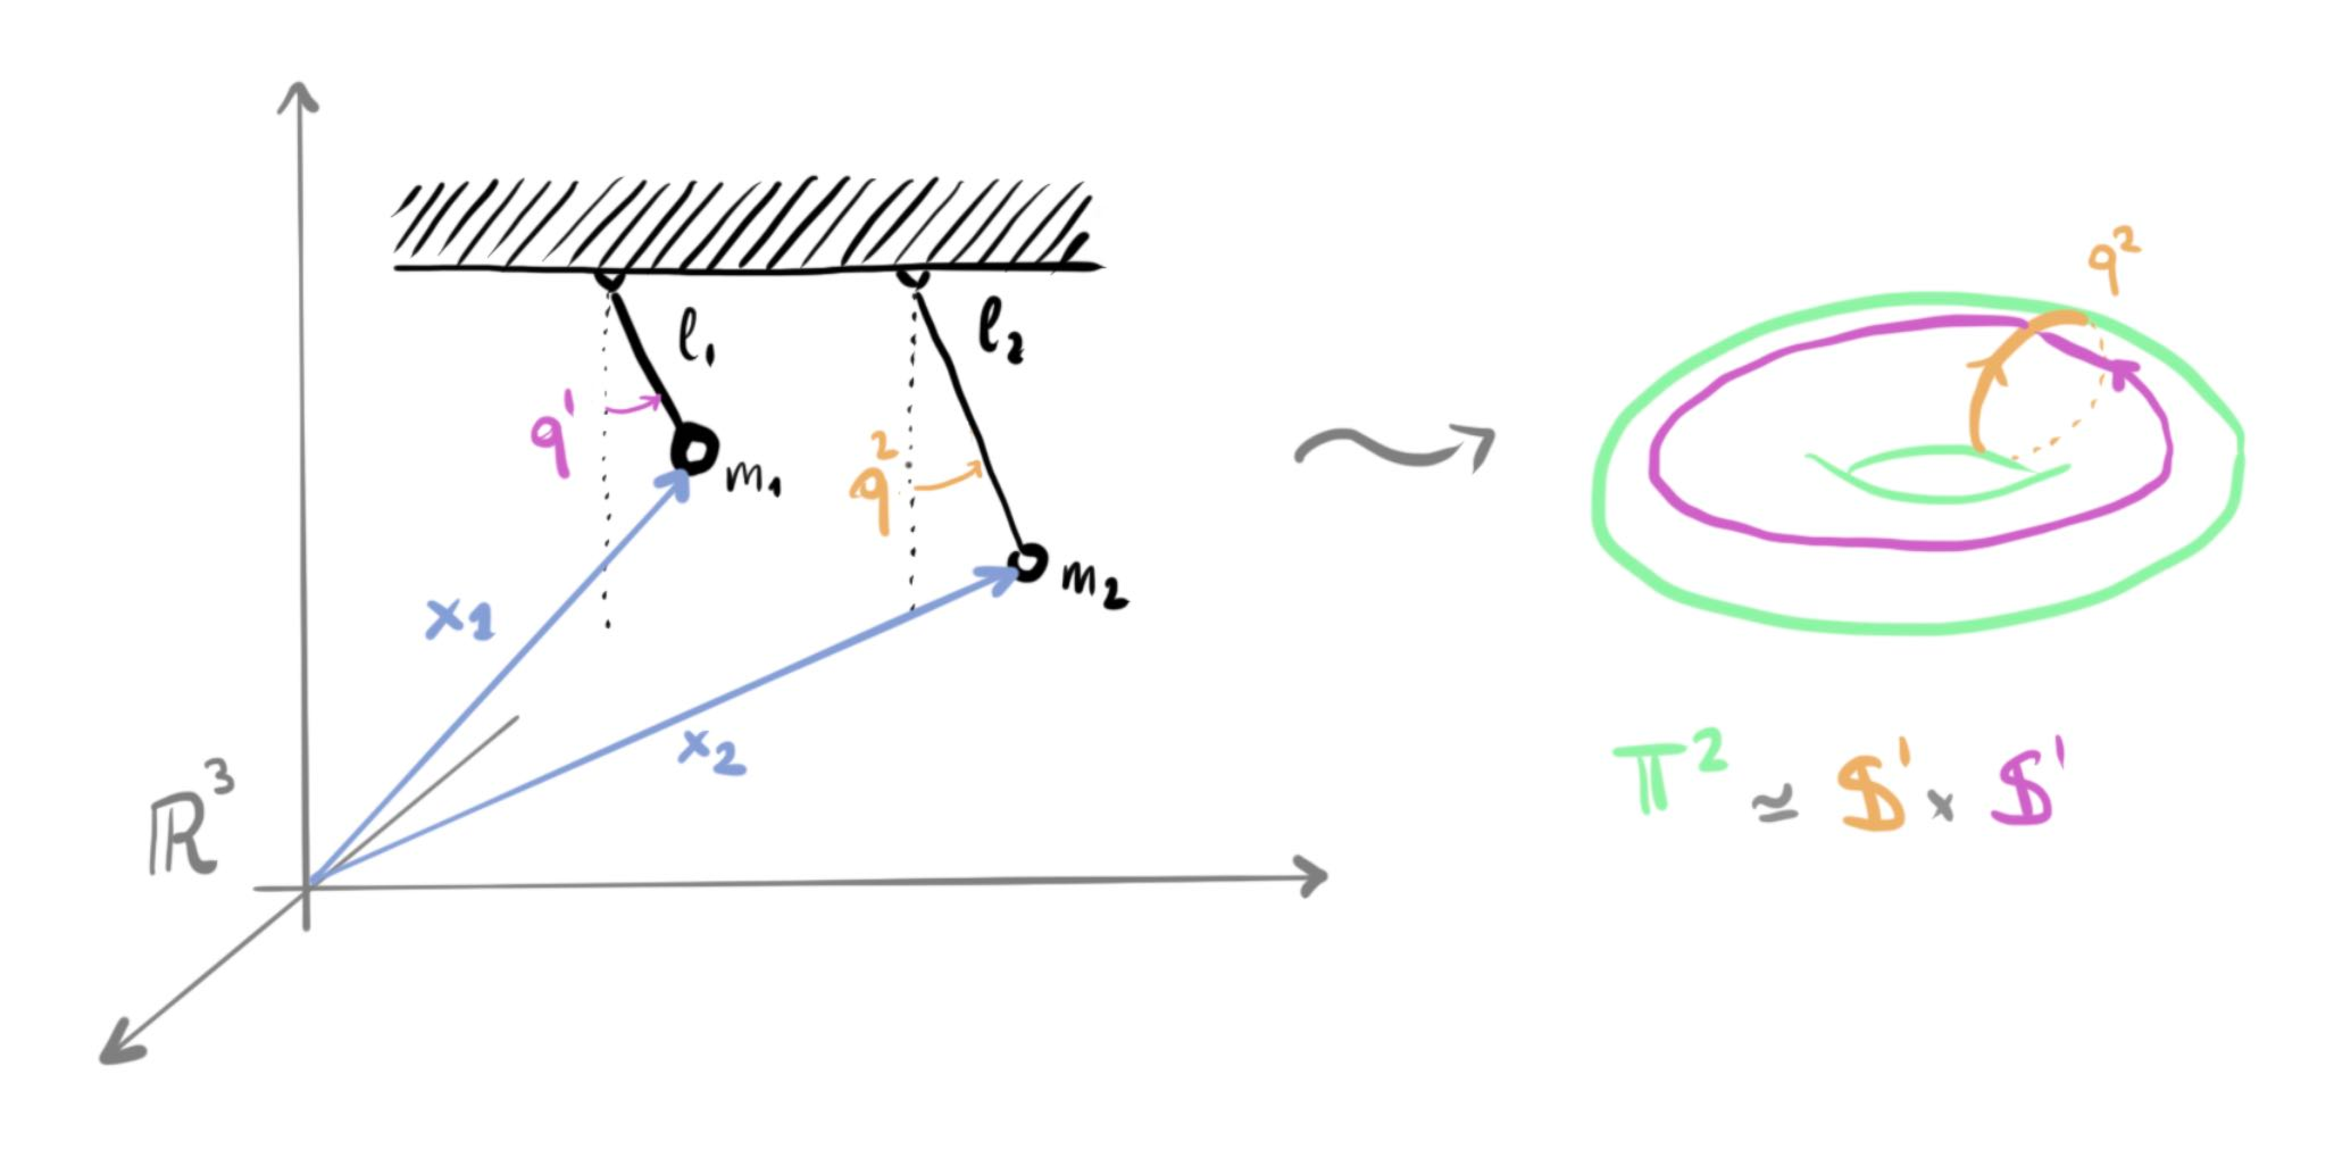
\includegraphics[width=0.9\linewidth,trim={0 1cm 0 1cm}, clip]{{images/HM-1.1}.pdf}
\end{figure}

We say that a system of $N$ particles has \emph{$n$ degrees of freedom} if we need $n$ independent parameters to uniquely specify the system configuration\footnote{As Example~\ref{example:gcoords} shows, the $n$ degrees of freedom do not have to be the cartesian coordinates of the point particles.}. We call \emph{generalized coordinates} any set of $n$ parameters $q = (q^1, \ldots, q^n)$ that uniquely determine the configuration of a system with $n$ degrees of freedom, and \emph{generalized velocities} their time derivatives $\dot q = (\dot q^1, \ldots, \dot q^n)$. The \emph{state} of the system is then characterized by the set of (generalized) coordinates and velocities $(q, \dot q) = \left(q^1, \ldots, q^n,\dot q^1, \ldots, \dot q^n\right)$.

If you recall differential geometry, you may (correctly) guess that the generalized coordinates will be points on some differentiable manifold $q\in M$ and the state will be a point in its tangent bundle $(q, \dot q)\in TM$, i.e. $\dot q \in T_q M$ (see also section~\ref{sec:lagrangianonmanifold}).
\medskip

We have now all the elements to translate the \emph{Newtonian principle of determinacy} in mathematical terms. 
In 1814, Laplace \cite{book:laplace} wrote

\begin{quotation}
    We may regard the present state of the universe as the effect of its past and the cause of its future. An intellect which at a certain moment would know all forces that set nature in motion, and all positions of all items of which nature is composed, if this intellect were also vast enough to submit these data to analysis, it would embrace in a single formula the movements of the greatest bodies of the universe and those of the tiniest atom; for such an intellect nothing would be uncertain and the future just like the past would be present before its eyes.
\end{quotation}

In other words, this principle states that the initial state $\left(q(t_0), \dot q(t_0)\right)$ uniquely determines its evolution $\left(q(t),\dot q(t)\right)$ for $t > t_0$.
The Picard-Lindel\"of theorem\footnote{Also known as ``Existence and uniqueness of solutions of initial value problems''.} implies that the Newtonian principle of determinacy is locally satisfied\footnote{Modulo some minimal regularity requirements.} by the \emph{equations of motion} of the mechanical system, i.e., second order differential equations derived from Newton's law.

\subsection{Motion in one degree of freedom}

Before temporarily moving to Lagrangian mechanics, let's anticipate some of the concepts in some simple cases.

\begin{example}[Horizontal spring and pendulum]\label{ex:sprPen}
    Consider an idealized system consisting of a point particle of mass $m$ attached to a spring with stiffness $k$, sliding on a frictionless surface.
    Assume that the motion is one-dimensional along the axis of the spring and let $x$ denote the displacement of the system from its equilibrium position, i.e., the position in which the spring is completely at rest: not compressed nor extended. We consider this system to exclude gravitational forces from the picture.
    
    Hooke's law states that the restoring force $F$ exerted by the spring on whatever is pulling its free end scales linearly with respect to the distance it's been pulled: i.e., $F(x) = - k x$. According to \eqref{eq:newton}, then, the motion of the point particle is given by
    \begin{equation}\label{eq:spring}
        m \ddot{x} = - k x \qquad\mbox{or}\qquad \ddot{x} = - \omega^2 x \quad\mbox{where } \omega = \sqrt{k/m}.
    \end{equation}
    The solution, $x(t)$, is generally described by 
    \begin{equation}\label{eq:springsol}
        x(t) = R \cos(\omega t + \phi),
    \end{equation} with the unknowns $R$ and $\phi$ uniquely prescribed by the initial conditions
    \begin{equation}
        x(0) = R\cos(\phi) \qquad\mbox{and}\qquad \dot x(0) = -\omega R \sin(\phi).
    \end{equation}
    Clearly, once we know the initial conditions, the full evolution of the solution $x(t)$ is known, in agreement with Newton's principle of determinacy.
\medskip

    Consider, now, a point particle of mass $m$ attached to a pivot on the ceiling via a rigid rod of length $l$.
    Assume the motion is frictionless and happening only in the vertical direction.
    Let $x$ denote the angle of displacement of the system from its equilibrium position, i.e., the lowest point on the arc of motion. Take the angle at equilibrium to be zero, with positive sign on the right hand side of the vertical, and negative on the left.
    
    The force acting on the pendulum is Earth's gravitational attraction. According to \eqref{eq:newton}, then, the motion of the point particle is given by
    \begin{equation}
        m l \ddot{x} = - m g \sin(x) \qquad\mbox{or}\qquad \ddot{x} = - \omega^2 \sin(x) \quad\mbox{where } \omega = \sqrt{g/l}.
    \end{equation}
    Here, $g \approx 9.8 m s^2$ denotes the gravitational acceleration.
    
    Although it is possible to solve the equation of motion of the pendulum by means of elliptic integrals, this is rather cumbersome.
    Under certain conditions, when $\sin x \approx x$, we can actually avoid doing this and instead we use the equation of the spring as a model for the pendulum oscillation via the so-called called \emph{small oscillations}.
    We will come back to this later on.
\end{example}

\begin{example}[Idealized motion of the Earth around the Sun]\label{ex:Kepler0}

    Let us approximate the Sun with a point particle of mass $M$ positioned at the origin $\bm{0}\in\R^3$ of the Euclidean space. In this solar system, with the Sun fixed at the origin, we will describe the Earth by a point particle of mass $m$ whose position (and motion) is described by a vector $\bx(t)\in\R^3$.

    Due to our choice of coordinates, the gravitational attraction of the Sun acts in direction $-\bx(t)$. \emph{Newton's law of universal gravitation} says that such a force is proportional to
    \begin{equation}
        \frac{GmM}{\|\bm{0}-\bx(t)\|^2} = \frac{GmM}{\|\bx(t)\|^2},
    \end{equation}
    where $G \sim 6.674 \cdot 10^{-11} \frac{m^3}{s^2\,kg}$ is called the \emph{gravitational constant}.
    Once we collect all the elements into Newton's second law \eqref{eq:newton}, we obtain the equation of motion
    \begin{equation}\label{eq:keplerex}
        m \ddot{\bx}(t) = - G\frac{mM}{\|\bx(t)\|^2} \frac{\bx(t)}{\|\bx(t)\|}.
    \end{equation}
    This is an autonomous second order ordinary differential equation on the configuration space $\R^3\setminus\big\{\bm{0}\big\}$.
    Providing the initial conditions $\bx(0)=\bx_0$ and $\dot{\bx}(0)=\bv_0$, we can explicitly solve \eqref{eq:keplerex}.

    Behind differential equations in classical mechanics lies a surprising geometrical structure in which conserved quantities play a special role.
    These can help to obtain extensive insights on the solution of classical equations of motion without the need to explicitly solve the equations (which would be, in general, impossible).
    
    On the tangent bundle $(\R^3\setminus\big\{\bm{0}\big\})\times\R^3$, let us define the total energy
    \begin{equation}\label{eq:energyKepler}
        E(\bx,\bv) = \frac{1}{2}m\|\bv\|^2 - \frac{GmM}{\|\bx\|},
    \end{equation}
    the angular momentum
    \begin{equation}
        L(x,v) = m \bv \wedge \bx,
    \end{equation}
    and the Laplace-Runge-Lenz vector
    \begin{equation}
        A(x,v) = m \bv \wedge L(\bx, \bv) + \frac{G m^2 M^2}{m+M} \frac{\bx}{\|\bx\|}.
    \end{equation}
    Along the solutions of \eqref{eq:keplerex}, let us define $E(t):=E(\bx(t),\dot\bx(t))$ and, similarly, $L(t)$ and $A(t)$. Then, there exist solutions such that $L(t) = L(0) \neq 0$ for all times, and also $E(t) = E(0)$ and $A(t) = A(0)$. Furthermore, a solution that lives on the ``submanifold'' defined by
    \begin{equation}
        \begin{aligned}
            \big\{
            &(\bx, \bv)\in (\R^3\setminus\big\{\bm{0}\big\})\times\R^3 \;\mid\\
            &\;
            E(\bx,\bv) = E(\bx_0, \bv_0),\;
            L(\bx,\bv) = L(\bx_0, \bv_0),\;
            A(\bx,\bv) = A(\bx_0, \bv_0)
        \big\},
        \end{aligned}
    \end{equation}
    must be a conic of the following type
    \begin{equation}
    \begin{split}
        \mbox{ellipse} \quad \mbox{if} \quad E(t) = E(0) < 0, \\
        \mbox{parabola} \quad \mbox{if} \quad E(t) = E(0) = 0, \\
        \mbox{hyperbola} \quad \mbox{if} \quad E(t) = E(0) > 0.
    \end{split}
    \end{equation}

    This is an example of a central force field, and is one of the most prominent and most important examples in this course.
    The impatient reader can find in \cite[Ch. 1]{book:knauf} a nice and compact derivation of Kepler's laws and the invariants above from \eqref{eq:keplerex} and its solutions.
\end{example}

\section{Hamilton's variational principle}\label{sec:varpri}

\begin{tcolorbox}
    Throughout this section we assume that our system has $n$ degrees of freedom whose configuration space is $\R^n$.    
\end{tcolorbox}
We will see that the generalization to manifolds is almost immediate.

In order to leave more space to discuss Hamiltonian systems and their geometry, we will be brief in our account of Lagrangian mechanics and calculus of variations. For a more detailed account refer to \cite[Part II]{book:arnold}.
This, however, should not confuse you: Lagrangian mechanics plays a role as large as Hamiltonian mechanics in the development of classical mechanics.

In fact, one should not be surprised if there are many sources claiming that the most general formulation of the equations of motion in classical mechanics comes from the \emph{principle of least action} or \emph{Hamilton's variational principle}. Indeed, as we will see this sits at the roots of Lagrangian mechanics and the Euler-Lagrange equations.

According to this principle, the equations of motion of a mechanical system are characterized by a function $L \equiv L(q, \dot q, t) : T\R^n \times \R \to \R$, called the \emph{lagrangian (function)} of the system.

\begin{example}
    The lagrangian of a non-relativistic particle with mass $m > 0$ in a potential $U : \R^n \to \R$ is
    \begin{equation}
        L(q, \dot q, t) = \frac12 m \|\dot q\|^2 - U(q),
    \end{equation}
    which is the difference between the so-called kinetic energy of the particle and its so-called potential energy.
    We will come back to this shortly.
\end{example}

Given a curve $\gamma:[t_1, t_2] \to \R^n$, we define the \emph{action} functional
\begin{equation}\label{eq:Laction}
    S[\gamma] := \int_{t_1}^{t_2} L(\gamma(s), \dot \gamma(s), s) \d s.
\end{equation}

\begin{tcolorbox}
    Assume that the configuration of our system is $q_1 = (q_1^1, \ldots, q_1^n)$ at an initial time $t=t_1$ and $q_2 = (q_2^1, \ldots, q_2^n)$ at a final time $t = t_2$. The \emph{principle of least action}, or \emph{Hamilton's principle}, states that the evolution of our system in the time interval $[t_1, t_2]$ corresponds to the curve $q(t)$ which is the critical point of the action functional $S[q]$ on the space of curves $q(t)$ with $q(t_1) = q_1$ and $q(t_2) = q_2$.
\end{tcolorbox}

To make this precise, we will need to recall some preliminary concepts and make sense of differentiation in $\infty$-dimensional spaces.

Let $X$ and $Y$ be Banach spaces\footnote{Banach space: complete normed vector space.}  and $G\subset X$ an open subset of $X$.
A function $f: G \to Y$ is call \emph{Fr\'echet differentiable} at $x\in G$, if there exists a bounded linear operator $A: X \to Y$, such that\footnote{Here, $g = o(\|h\|_X)$ if 
\begin{equation}
    \lim_{\|h\| \to 0} \frac{\|g(h)\|_Y}{\|h\|_X} = 0.
\end{equation}
}
\begin{equation}\label{eq:frechetdiff}
    f(x+h) = f(x) + Ah + o(\|h\|_X)
\end{equation}
for any $h$ in a sufficiently small neighborhood of $0\in X$. Alternatively, you can say asymptotically as $\|h\|_X\to 0$.

As in the finite-dimensional case, $A$ is uniquely determined and is called the \emph{Fr\'echet derivative} of $f$ at $x$ and is denoted $D f(x)$.

\begin{remark}
    \begin{enumerate}
        \item In the finite dimensional setting, Fr\'echet differentiability corresponds to total differentiability. As with the finite dimensional case, Fr\'echet's differentiability implies the continuity of the mapping.
        \item The analogy with the finite dimensional case goes further. Indeed, the chain rule, mean value theorem, implicit functions theorem, inverse mapping theorem and statements about local extremes with and without constraints, all hold also for differentiable functions on Banach spaces.
        \item Requiring the operator $A$ to be bounded is crucial. In $\infty$-dimensional normed spaces, the linearity of an image does not imply continuity.
        \item In calculus of variation, the curve $h$ from the small neighborhood of $0\in X$, is usually called a variation and denoted $\delta x$.
    \end{enumerate}
\end{remark}

Let $f: X \to \R$ be a (Fr\'echet) differentiable function and $X_0 \subset X$ be a subspace of $X$. Then $\gamma_\star$ is a \emph{critical point} of $f$ with respect to $X_0$ if
\begin{equation}
    Df(\gamma_\star)\Big|_{X_0} = 0, \quad\mbox{i.e.}\quad
    Df(\gamma_\star)h = 0 \mbox{ for all } h\in X_0.
\end{equation}

It is possible to show that the space of curves 
\begin{equation}
    X := \big\{ \gamma: [t_1, t_2] \to M \mid \gamma \mbox{ is twice continuously differentiable}\big\},
\end{equation} equipped with the norm
\begin{equation}
    \|\gamma\|_X :=
    \|\gamma\|_\infty + \|\dot \gamma\|_\infty + \|\ddot \gamma\|_\infty,
\end{equation}
is a Banach space, and $X_0 = \big\{h\in X \mid h(t_1) = h(t_2) = 0\big\}$ with the induced norm, is a Banach subspace of $X$. 

Therefore, the action defined above is a functional
\begin{equation}
    S : X \to \R,\qquad \gamma \mapsto S[\gamma],
\end{equation}
and the evolution of the system is described by the critical points with respect to $X_0$ of $S$ on the space of $\gamma \in X$ with prescribed endpoints.

\begin{theorem}
    Let $L = L(q, \dot q, t) : T\R^{n}\times\R = R^{n}\times R^{n}\times R \to \R$ be differentiable.
    The equations of motion for the mechanical system with lagrangian $L$ satisfy the \emph{Euler-Lagrange equations}
    \begin{equation}\label{eq:eulerlagrange}
        \frac{\d}{\d t}\frac{\partial L}{\partial \dot q^i} - \frac{\partial L}{\partial q^i} = 0, \quad i=1,\ldots n.
    \end{equation}
\end{theorem}

\begin{proof}
    We need to show that any critical point of $S$ with respect to $X_0$ has to satisfy \eqref{eq:eulerlagrange}.

    First of all observe that for small $h$, we get
    \begin{equation}
        \begin{split}
            S(\gamma + h) &= \int_{t_1}^{t_2} L(\gamma + h, \dot \gamma + \dot h, s) \d s \\
            &= \int_{t_1}^{t_2} % not clear how this step happens, specifically where the inner product comes from, maybe a comment on the procedure beforehand
                L(\gamma, \dot \gamma, s) \d s \\
            &\quad + \int_{t_1}^{t_2} \left[
                \left\lag
                    \frac{\partial L}{\partial q}(\gamma, \dot \gamma, s),\;
                    h(s)
                \right\rag
                + \left\lag
                    \frac{\partial L}{\partial \dot q}(\gamma, \dot \gamma, s),\;
                    \dot h(s)
                \right\rag
            \right] \d s \\
            &\quad + O(\|h\|^2_X),
        \end{split}
    \end{equation}
    where the inner product $\lag\cdot,\cdot\rag$ is to the usual scalar product in $\R^n$.

    Therefore,
    \begin{equation}
        \begin{split}
            S(\gamma+h) - S(\gamma) &= \int_{t_1}^{t_2} \left[
                \left\lag\frac{\partial L}{\partial q}(\gamma, \dot \gamma, s),\; h(s)\right\rag
                + \left\lag\frac{\partial L}{\partial \dot q}(\gamma, \dot \gamma, s),\; \dot h(s)\right\rag
            \right] \d s\\
            &\quad + O(\|h\|^2_X)\\
            &= \left\lag\frac{\partial L}{\partial \dot q}(\gamma, \dot \gamma, s),\; h(s)\right\rag \Big|_{t_1}^{t_2} \\
            &\quad + \int_{t_1}^{t_2} \left\lag
                \frac{\partial L}{\partial q}(\gamma, \dot \gamma, s)
                - \frac{\d}{\d s}\frac{\partial L}{\partial \dot q}(\gamma, \dot \gamma, s)
            ,\; h(s)\right\rag \d s\\
            &\quad + O(\|h\|^2_X).
        \end{split}
    \end{equation}

    The differential $DS(\gamma): X \to \R$ can now be read from the equation above and is well--defined and is a bounded linear operator for all $\gamma\in X$.

    For $h\in X_0$, the first term $\left\lag\frac{\partial L}{\partial \dot q}(\gamma, \dot \gamma, s),\; h(s)\right\rag\Big|_{t_1}^{t_2}$ has to vanish. Therefore, for $\gamma$ to be a critical point for $S$ it follows that the inner product
    \begin{equation}
        \left\lag
            \frac{\partial L}{\partial q}(\gamma, \dot \gamma, s)
            - \frac{\d}{\d s}\frac{\partial L}{\partial \dot q}(\gamma, \dot \gamma, s)
        ,\; h(s)\right\rag = 0 \quad\mbox{for all } h\in X_0.
    \end{equation}

    Our choice of $h$ is arbitrary, so after a relabelling of the time, this implies
    \begin{equation}
        \frac{\partial L}{\partial q}(\gamma, \dot \gamma, t)
            - \frac{\d}{\d t}\frac{\partial L}{\partial \dot q}(\gamma, \dot \gamma, t) = 0,
    \end{equation}
    which, expanded, means
    \begin{equation}
        \frac{\d}{\d t}\frac{\partial L}{\partial \dot q^i}(\gamma, \dot \gamma, t) - \frac{\partial L}{\partial q^i}(\gamma, \dot \gamma, t) = 0, \quad i=1,\ldots n.
    \end{equation}
\end{proof}

\begin{remark}
    The solution $q=q(t)$ of the Euler-Lagrange equations is just a critical point of the $S$ functional:
    \begin{equation}
        S[q + \delta q] - S[q] = O(\|\delta q\|^2).
    \end{equation}
    It does \textbf{not} have to be a minimum. However, under some additional conditions it can be proven to be a \emph{local} minimum.
    For example, if the matrix of second derivatives
    \begin{equation}
        \left(
            \frac{\partial^2 L}{\partial\dot q^i \partial\dot q^j}
        \right)_{1\leq i,j\leq n}
    \end{equation}
    is positive definite.
    This case is thoroughly studied in calculus of variation and in some instances of differential geometry.
\end{remark}

\begin{corollary}
    If the lagrangian of the system is \emph{non--degenerate}, i.e., it satisfies the condition
    \begin{equation}
            \det \left(\frac{\partial^2 L}{\partial\dot q^i \partial\dot q^j}
        \right)_{1\leq i,j\leq n} \neq 0
    \end{equation}
    then it satisfies Newton's determinacy principle.
\end{corollary}

\begin{proof}
    For a non--degenerate lagrangian, the Euler-Lagrange equations can be rewritten in the form %by the implicit function theorem?
    \begin{equation}
        \ddot q^i = f^i(q,\dot q, t)
        := \Lambda^{ij}\left(\frac{\partial L}{\partial q^j} - \frac{\partial^2 L}{\partial \dot q^j \partial q^k} \dot q^k - \frac{\partial^2 L}{\partial\dot q^j \partial t}\right),
        \quad i=1,\ldots,n.
    \end{equation}
    Here, the sum over the repeated indices\footnote{For example, $y^{ji} x_i \equiv \sum_i y^{ji} x_i$} is implied and the matrix $\left(\Lambda^{ij}\right) = \left(\Lambda^{ij}(q, \dot q, t)\right)$ is the inverse to $\left(\frac{\partial^2 L}{\partial \dot q^i \partial \dot q^j}\right)$:
    \begin{equation}
        \Lambda^{ik} \frac{\partial^2 L}{\partial \dot q^k \partial \dot q^j} = \delta_{ij}.
    \end{equation}
\end{proof}

In other words, we can use Euler-Lagrange equations as the equations of motion of a mechanical system with non--degenerate lagrangian.

\begin{remark}\label{rmk:manylagrangians}
    \emph{The lagrangian of a mechanical system is defined only up to total derivatives}.
    Or, in other words, the equations of motion remain unchanged if we add a total derivative to the lagrangian function:
    \begin{equation}
        \tilde L(q,\dot q, t) = L(q, \dot q, t) + \frac{\d}{\d t} f(q,t).
    \end{equation}
    The action $\tilde S$ of a system with lagrangian $\tilde L$ is
    \begin{align}
        \tilde S[q] &= \int_{t_1}^{t_2} \tilde L(q, \dot q, t) \,\d t \\
        &= \int_{t_1}^{t_2} L(q, \dot q, t) \,\d t + \int_{t_1}^{t_2} \frac{\d}{\d t} f(q,t) \,\d t \\
        &= S[q] + f(q_2, t_2) - f(q_1, t_1).
    \end{align}
    As the additional $f$-dependent part is constant,
    \begin{equation}
        \tilde S[q+\delta q] - \tilde S[q]
        = S[q+\delta q] - S[q]
    \end{equation}
    and thus the critical points of the two actions are the same.

    Similarly, \emph{the lagrangian of a mechanical system does not change if it is multiplied by a constant factor: $\tilde L = \alpha L$}.

    As an aside, quantum mechanical systems no longer remain invariant under the transformations above. Transformations of the first type lead to rather subtle and interesting effects related to topology, while the number $\alpha$ is related to Planck's constant. 
    \medskip

    Coming back to our discussion: with so much freedom, how does one choose a normalization for the lagrangian then?
    One way, is by using the \emph{principle of additivity}.
    \begin{tcolorbox}
        Assume that a mechanical system is the combination of two subsystems, say $A$ and $B$.
        Let $L_A$ and $L_B$ be their respective lagrangian as if they were isolated (or \emph{closed}) systems.
        The principle of additivity says that by moving the two subsystems farther apart from each other, in the limit of infinite distance, the lagrangian of the full system tends to the limit lagrangian
        \begin{equation}
            L_{\lim} = L_A + L_B.
        \end{equation}
    \end{tcolorbox}
\end{remark}

\subsection{Dynamics of point particles: from Lagrange back to Newton}\label{sec:dynamicspps}

Mechanical laws for the same system can look very differently from each other, with varying degrees of simplification or complication: think for example as the motion of planets in a geocentric system of coordinates.
There is a system of coordinates that simplifies our life the most: the \emph{inertial} coordinate system.

\begin{tcolorbox}
The \emph{galilean principle of relativity} says that there exist coordinate systems, called inertial, with the following two properties
\begin{enumerate}
    \item all the laws of nature at all moments of time are the same in all inertial coordinate systems;
    \item all coordinate systems in uniform rectilinear motion with respect to an inertial one are themselves inertial.
\end{enumerate}
\end{tcolorbox}

Although the discussion on the group theoretical aspects of classical mechanics, which very much relates to this discussion, is very interesting and fascinating we will not discuss it here further, we leave \cite{book:marsdenratiu} as an interesting reference.

For our concerns, an inertial system of coordinates on the galilean space-time is an isomorphism with the ``standard'' galilean structure $\R\times\R^3$.
If $(t, \bx) \in \R\times \R^3$ is an element of the ``standard'' galilean space-time, we call \emph{galilean transformations} the transformations $(t,\bx) \to (\tilde t, \tilde{\bx})$ listed below
\begin{enumerate}
    \item translations: $\tilde t = t + t_0$, $\tilde{\bx} = \bx + \bx_0$, for $t_0\in\R$, $\bx_0\in\R^3$;
    \item rotations: $\tilde t = t$, $\tilde{\bx} = G\bx$ for $G\in O(3)$;
    \item uniform motions with velocity $\bm{v}\in\R^3$: $\tilde t = t$, $\tilde{\bx} = \bx + \bm{v} t$.
\end{enumerate}
Then, the galilean principle of relativity says that the lagrangian of a closed mechanical system is invariant, modulo the sum of total derivatives, with respect to the galilean transformations.

We will now see how we can derive Newton's laws from Hamilton's principle as a consequence of the galilean principle of relativity. For an alternative discussion on this topic see \cite[Chapters 1.1 and 1.2]{book:arnold}.

\begin{theorem}
The lagrangian of an isolated point particle in an inertial system of coordinates has the form 
\begin{equation}\label{eq:singleptlag}
    L(\bm{x}, \dot{\bm{x}}) = \frac{m\,\|\dot{\bm{x}}\|^2}2
\end{equation}
where $m$ is a constant called the \emph{mass} of the point particle.
\end{theorem}
\begin{proof}
    The invariance from translations implies that the lagrangian must be independent from $t$ and $\bx$, while the invariance from orthogonal transformations implies that it must be dependent on the square of the velocities:
    \begin{equation}
        L = L(\|\dot\bx\|^2), \quad \|\dot\bx\|^2 := \lag\dot \bx, \dot \bx\rag.
    \end{equation}
    The invariance with respect to uniform motion now implies that the lagrangian must actually be proportional to $\|\dot\bx\|^2$.
    Indeed, with the galilean transformation
    \begin{equation}
        \bx \mapsto \bx + \epsilon \bm{v}t,
    \end{equation}
    in the limit $\epsilon \to 0$, we get
    \begin{equation}
        L(\|\dot\bx\|^2) \mapsto L(\|\dot\bx\|^2) + 2\epsilon\,\lag\bm{v}, \dot\bx\rag\,\frac{\partial}{\partial \|\dot\bx\|^2}L(\|\dot\bx\|^2) + O(\epsilon^2).
    \end{equation}
    The invariance of the lagrangian implies that the linear term in $\epsilon$ should be a total derivative $\frac{\d }{\d t} f(t, \bx) = 2\,\lag\bm{v}, \dot\bx\rag\,L'(\|\dot\bx\|^2)$ but this can happen iff it's linear in $\|\dot\bx\|^2$, in particular this means that $L'(\|\dot\bx\|^2) = \mathrm{const} =: \frac{m}2$.
    
    Finally, for any constant value $m$, the lagrangian \eqref{eq:singleptlag} is invariant with respect to $\bx \mapsto \bx + \bm{v}t$:
    \begin{equation}
        \frac{m \|\dot\bx\|^2}2 \mapsto
        \frac{m \|\dot\bx\|^2}2 + m\,\lag\bm{v},\dot\bx\rag + \frac{m \bm{v}^2}2
        = \frac{m \|\dot\bx\|^2}2 + \frac{\d }{\d t}\left(m\,\lag\bm{v},\bx\rag + \frac{m \bm{v}^2 t}2\right).
    \end{equation}
\end{proof}

\begin{corollary}[Newton's first law]
In an inertial frame of reference, an isolated point particle either does not move or is in uniform motion with constant velocity.
\end{corollary}
\begin{proof}
    It follows immediately by computing the Euler-Lagrange equations for \eqref{eq:singleptlag}:
    \begin{equation}
        \frac{\d}{\d t} \frac{\partial L}{\partial \dot x^i} - \frac{\partial L}{\partial x^i} = m \ddot x^i = 0, \qquad i=1,2,3.
    \end{equation}
\end{proof}

Remembering the additive property of the lagrangians, we can show that for a system of $N$ particles, which do not interact, the lagrangian is the sum
\begin{equation}\label{eq:freel}
    L = \sum_{k=1}^N \frac{m_k \|\dot{\bx}_k\|^2}{2}.
\end{equation}
We call lagrangians of this form \emph{free}.

\begin{remark}
    The above definition of mass becomes only meaningful, when we take the additive property into account.
    A lagrangian can always be multiplied by an arbitrary constant without affecting the equations of motion;
    such multiplication then amounts to a change in the unit of mass.
    The ratios of the masses remain unchanged by this and it is only these ratios which are physically meaningful.
\end{remark}

To include interaction between the points in this picture, we need to add to the free lagrangian \eqref{eq:freel} a function $-U(\bx_1, \ldots, \bx_N)$ which depends on the nature of the interactions:
\begin{equation}\label{eq:mechlag}
    L := T-U := \sum_{k=1}^N \frac{m_k \|\dot{\bx}_k\|^2}{2} -U(\bx_1, \ldots, \bx_N).
\end{equation}
The first sum, $T = \sum_{k=1}^N \frac{m_k \|\dot{\bx}_k\|^2}{2}$, is called \emph{kinetic energy} of the particles, while the function $U = U(\bx_1, \ldots, \bx_N)$ is called \emph{potential energy}. Lagrangians of the form $T-U$ are often called \emph{natural}.

\begin{theorem}
    The equations of motion of a system of $N$ point particles with natural lagrangian \eqref{eq:mechlag} are of the form
    \begin{equation}\label{eq:newton2}
        m_k \ddot\bx_k = \bm{F}_k, \quad k=1,\ldots,N
    \end{equation}
    where $\bm{F}_k = -\frac{\partial U}{\partial \bm{x}_k}$, $\quad k=1,\ldots,N$.
\end{theorem}

The vector $\bm{F}_k$ is called the \emph{force} acting on the $k$-th point particle, and you should immediately recognize \emph{Newton's second law} in \eqref{eq:newton2}.

\begin{exercise}\label{ex:N3l1}
    Prove \emph{Newton's third law}, i.e. for each of the $k$ point particles it holds
    \begin{equation}
        \bm{F}_k = -\sum_{j\neq k} \bm{F}_j.
    \end{equation}
    (Hint: use the invariance with respect to spacial translations.)
\end{exercise}

\begin{remark}
\begin{enumerate}
    \item Mechanical systems are \emph{reversible}: they are also invariant with respect to the transformation $t\mapsto -t$.
    \item If you consider systems in interaction with the environment, you end up with lagrangians that are no longer invariant with respect to galilean transformations and can explicitly depend from time.
\end{enumerate}
\end{remark}

\begin{example}
    Consider the vertical motion of a point particle of mass $m$ in the external field with potential $U(z) = m g z$. Here $g$ is the gravitational acceleration $g \sim 9.8 m s^{-2}$. The natural lagrangian of the system is
    \begin{equation}
        L = \frac{m\dot z^2}2 - mgz,
    \end{equation}
    which corresponds to the equation of motion $\ddot z = -g$: this is the equation of motion of a point particle in free fall towards Earth. In agreement with Galileo's law, the acceleration is constant and does not depend from the mass.
\end{example}

\begin{example}\label{ex:kepler1}
    The motion of $N$ point particles with masses $m_1, \ldots, m_N$ in their gravitational field, is described by the lagrangian
    \begin{equation}
        L = \sum\frac{m_k \|\dot{\bx}_k\|^2}{2} + \sum_{k < l} G \frac{m_k m_l}{\|\bx_k - \bx_l\|},
    \end{equation}
    where $G$ is the gravitational constant.

    To study the \emph{approximate} description of the motion of a planet of mass $m$ around the Sun, which has mass $M \gg m$, one can assume the effects of the planet on the Sun to be negligible and ignore the interaction with the other planets.

    In such a case, the motion of the planet is described by the lagrangian of a point particle with a Newtonian gravitational potential
    \begin{equation}
        L = \frac{m\|\dot\bx\|^2}{2} + \frac{G M m}{\|\bx\|},
    \end{equation}
    whose equation of motion should remind you of \eqref{eq:keplerex} from Example~\ref{ex:Kepler0}.
\end{example}

To understand better why $T$ in \eqref{eq:mechlag} is called kinetic energy, it is useful to look at its relation with Newton's second law \eqref{eq:newton2}:
\begin{equation}
    \frac{\d}{\d t} T
        = m \lag\dot \bx(t), \ddot \bx(t)\rag
        = \left\lag\dot \bx(t), \bm{F}(\bx(t))\right\rag.
\end{equation}
This confirms the intuitive notion that the kinetic energy should increase if a force pushes the particle in the direction of the current motion and should decrease when it pulls the particle in the opposite direction.

There is more, in fact
\begin{equation}
    T(t_1) - T(t_0) = \int_{t_0}^{t_1} \left\lag\dot \bx(t), \bm{F}(\bx(t))\right\rag\; \d t,
\end{equation}
which is to say that the change of kinetic energy is equal to the \emph{work} done by the force, i.e. the integral of $\bm{F}$ along the curve $\bx(t)|_{t\in[t_0, t_1]}$. The name comes from the fact that, physically, you can think of $F(\bx) \cdot \d\bx$ as the infinitesimal contribution of the vector field to the acceleration.

\begin{remark}
For $N=1$, Stokes' theorem implies that the integral above is independent from the path between $\bx_0 = \bx(t_0)$ and $\bx_1 = \bx(t_1)$ if and only if $\curl \bm{F} = 0$, which in turn is true if and only if there is a $U:\R^3\to\R$ such that $\bm{F} = -\nabla U$.

In fact, this is true in any dimension by using the general version of Stokes' theorem: the work done by the force depends only on the endpoints of the integral if and only if there is $U:\R^n\to\R$, unique up to an additive constant, such that $\bm{F} = -\nabla U$.

You can read about this also in \cite[Chapter 2.5]{book:arnold} and \cite[Theorem 6.3 and 8.1]{book:knauf}.
\end{remark}

Forces that can be written in the form $\bm{F} = -\frac{\partial U}{\partial \bm{x}}$, for some function $U$, are called \emph{conservative}.
We will understand better why in a couple of sections.

Not all the forces in nature are conservative, and in that case the results of this section do not directly apply.
We don't have to go very far to see an example of this, but we can also see that the lagrangian approach can be easily extended to include non-conservative forces.

\begin{example}\label{exa:magnetic}
    Mechanical systems affected by an external magnetic field $\bm B$ can be described in the lagrangian formalism by adding a linear term in the velocities to a natural lagrangian \eqref{eq:mechlag}:
    \begin{equation}\label{eq:magLag}
        \tilde L = L + \frac ec \sum_{i=1}^N \lag\bm A(\bx_i), \dot \bx_i\rag.
    \end{equation}
    Here the constant $e$ is the electric charge of the point particles and $c$ is the speed of light in vacuum.
    The magnetic field is given by $\bm B = \curl \bm A$, the vector field $\bm A$ is called magnetic vector potential.
    
    We will not see this in the course, but magnetic phenomenons have a natural description only in the relativistic approach. We see a hint of this fact here, in that \eqref{eq:magLag} is not invariant with respect to the galilean transformations.
    
    \begin{exercise}\label{exe:magnetic}
        Show that the equations of motion \eqref{eq:newton2} corresponding to a magnetic lagrangian \eqref{eq:magLag} are given by
        \begin{equation}
            m_k \ddot\bx_k = \bm{F}_k + \frac ec \dot\bx_k \wedge \bm B(\bx_k)
        \end{equation}
        where the exterior product corresponds to the usual vector product in $\R^3$ and, as mentioned above, $\bm B = \curl \bm A$ is the magnetic field.

        The additional term $\frac ec \dot\bx_k\wedge \bm B(\bx_k)$ is the \emph{Lorenz force} acting on the $k$th particle of charge $e$ immersed in the magnetic field $\bm B$.

        For a beautiful geometric discussion of this problem, refer to \cite[Chapter 8.3]{book:amr} (which is Chapter 9.3 in the forthcoming 3rd edition).
    \end{exercise}
    
    Note that the magnetic vector potential is not unique!
    For any function $f$, the transformation
    \begin{equation}
        \bm A \mapsto \bm A + \frac{\partial f}{\partial \bx}
    \end{equation}
    will produce the same field.
    This is known as \emph{gauge transformation}.
    Under this transformation the lagrangian is transformed as
    \begin{equation}
        \tilde L \mapsto \tilde L + \frac{e}{c} \frac{\d f}{\d t}
    \end{equation}
    but we know that the equations of motion remain invariant under the addition of a total derivative to the Lagrangian.
    The concept of gauge invariance is central in lots of modern physics.
\end{example}

\section{Euler-Lagrange equations on smooth manifolds}\label{sec:lagrangianonmanifold}

Before entering into the actual definition, let's play a bit with what we already have.

We introduced the generalized coordinates in the first section of this chapter but by now, we don't yet know if and how the lagrangian formalism translates into that language.
Let's consider a natural lagrangian for a system of $N$ particles, so in $\R^{3N}$, with equal mass $m=1$.
If we describe the motion in terms of generalized coordinates
\begin{equation}
    \bx_k = \bx_k(q^1, \ldots, q^{3N}), \quad k=1,\ldots,N,
\end{equation}
a direct application of the chain rule will allow us to rewrite the lagrangian as
\begin{equation}
    L = T - U,
    \qquad\mbox{where}
    \begin{cases}
        T:= \frac12 g_{kl}(q)\dot q^k \dot q^l, \quad U = U(q),\\
        g_{kl} (q) := \sum_{j=1}^N \left\lag\frac{\partial\bx_j}{\partial q^k}, \frac{\partial \bx_j}{\partial q^l}\right\rag
    \end{cases}
\end{equation}
and, again, we used Einstein summation convention.

If, for example, we consider a free one-particle lagrangian in cartesian coordinates $\bx = (x,y,z)$,
\begin{equation}
    L = \frac m2 (\dot x^2 + \dot y^2 + \dot z^2),
\end{equation}
in cylindrical coordinates $(r,\phi,z)$ it would read
\begin{equation}
    L = \frac m2 (\dot r^2 + r^2 \dot \phi^2 + \dot z^2),
\end{equation}
while in spherical coordinates $(r,\phi,\theta)$, see also Figure~\ref{fig:sphcoords}, it would become
\begin{equation}
    L = \frac m2 (\dot r^2 + r^2 \dot \theta^2 + r^2 \sin^2(\theta) \dot \phi^2).
\end{equation}

The term $g_{kl} (q)$ should also ring a bell in the context of this example: the arc length $s$ of a parametrized curve $q(t) : [t_1,t_2] \to \R^3$, is computed as
\begin{equation}\label{eq:arclen}
    \begin{aligned}
        s = \int_{t_1}^{t_2} \sqrt{\d s^2} = \int_{t_1}^{t_2} \sqrt{g_{kl}(q)\dot q^k \dot q^l} \;\d t,\quad
        g_{kl} (q) = \left\lag\frac{\partial\bx}{\partial q^k}, \frac{\partial \bx}{\partial q^l}\right\rag.
    \end{aligned}
\end{equation}
We can compute what $\d s^2$ looks like for the three coordinates above.
In cartesian coordinates, we have
\begin{equation}
    \d s^2 = \d x^2 + \d y^2 + \d z^2,
\end{equation}
while in cylindrical coordinates
\begin{equation}
    \d s^2 = \d r^2 + r^2 \d \phi^2 + \d z^2,
\end{equation}
and in spherical coordinates, see Figure~\ref{fig:sphcoords},
\begin{equation}\label{eq:spharc}
    \d s^2 = \d r^2 + r^2 \sin^2(\theta) \d \phi^2 + r^2 \d \theta^2.
\end{equation}
You can see that there is a striking resemblance between the squared arc length elements and the lagrangian functions above.

Let's consider the more general situation of local coordinates $(q^1, \ldots, q^n)$ on a smooth manifold $M$.
We will only recall the main terminology here, for a review of these concepts refer to \cite[Chapter 4.18]{book:arnold}, \cite[Appendix A]{book:knauf}, \cite[Chapter 4]{book:marsdenratiu}, your favourite book of differential geometry\footnote{Mine is \cite{book:lee}, which is freely accessible through the University library} or my beautiful\footnote{If I do say so, myself.} lecture notes \cite{lectures:aom:seri}.

We denote $T_q M$ the \emph{tangent space} of $M$ at $q$, and $TM = \cup_{q\in M}\{q\}\times T_q M$ the \emph{tangent bundle} of $M$. The latter is a smooth $2n$-dimensional manifold whose points are the pairs $(q,\dot q)\in TM$, where $q\in M$ and $\dot q\in T_q M$.

Local coordinates on $M$ are local diffeomorphisms $\phi:U\subset M\to \R^n$ over open sets $U\subset M$. If we have different local coordinates $\phi:U\subset M\to\R^n$, $\psi:V\subset M\to\R^n$ for a smooth manifold, we require on the intersection $W=U\cap V$ that their transition maps $\phi\circ\psi^{-1}:\psi(U\cap V)\to\phi(U\cap V)$ are also diffeomorphisms.

Local coordinates $(q^1,\ldots,q^n)$ on $M$ induce local coordinates $(q^1,\ldots,q^n,\dot q^1, \ldots,\dot q^n)$ on $TM$: for all $i=1,\ldots,n$ the coordinate $\dot q^i$ of the tangent vector $v\in T_qM$ is defined as
\begin{equation}
    \dot q^i(v) = v^i,\quad v = v^1\frac{\partial}{\partial q^1}+\cdots+v^n \frac{\partial}{\partial q^n}.
\end{equation}

To emphasize once more the importance of the chain rule in this business, a local change of coordinates on $M$ determines a special class of coordinate transformations on the tangent bundle which is linear with respect to the coordinates $\dot q$ on the fibers:
\begin{equation}
    \tilde q^i = \tilde q^i (q), \quad \dot{\tilde q}^i = \frac{\partial\tilde q^i}{\partial q^k}\dot q^k.
\end{equation}

\begin{exercise}[To review a bit of differential geometry that we will also need later on]\label{exe:coordinatesInd}
    Let $L=L(q,\dot q):TM \to \R$ be a smooth function. Show that the \emph{linear momenta}, i.e. the derivatives
    \begin{equation}
        p_i := \frac{\partial L}{\partial \dot q^i}, \quad i=1,\ldots,n,
    \end{equation}
    transform as components of the cotangent bundle $T^* M$ over $M$:
    \begin{equation}
        \tilde p_i = \frac{\partial q^k}{\partial {\tilde q}^i} p_k, \quad i=1,\ldots,n.
    \end{equation}
    Furthermore, show that the matrix of second derivatives with respect to the coordinates $\dot q$ of the lagrangian transforms as a $(0,2)$-tensor, i.e.
    \begin{equation}
        \frac{\partial^2 L}{\partial \dot{\tilde q}^i \partial \dot{\tilde q}^j} =
        \frac{\partial q^k}{\partial {\tilde q}^i}\frac{\partial q^l}{\partial {\tilde q}^j}
        \frac{\partial^2 L}{\partial \dot{q}^k \partial \dot{q}^l}.
    \end{equation}
    \emph{Hint: use Euler-Lagrange equation.}
\end{exercise}

The manifold $M$ is called \emph{configuration space}, its tangent bundle $TM$ is called \emph{state space}. The dimension $n$ of the configuration space is the \emph{number of degrees of freedom} of the mechanical system.  A smooth function $L=L(q,\dot q, t)$ on $TM\times R$ is called the \emph{lagrangian} of the mechanical system. The lagrangian is called \emph{non--degenerate} if
\begin{equation}
    \det %\left(
        \left(\frac{\partial^2 L}{\partial \dot{q}^i \partial \dot{q}^j}\right)_{1\leq i,j\leq n} 
    %\right)
    \neq 0.
\end{equation}

Thanks to the second part of the exercise above, the class of non--degenerate lagrangians is  independent of the choice of local coordinates on the configuration space.

To simplify the discussion and the geometrical description, we now assume that the lagrangian is non--degenerate and that it does not explicitly depend on time.
As for the euclidean case, given a lagrangian $L$ we can define a functional $S$ on the space of smooth curves $q(t): [t_1,t_2] \to M$ with $q(t_1) = q_1$ and $q(t_2) = q_2$ as the integral
\begin{equation}
    S[q] = \int_{t_1}^{t_2} L(q,\dot q) \d t.
\end{equation}
It turns out\footnote{Truth be told, we are hiding some extra complications involving infinite dimensional manifolds here, for a full account of the theory involved you can refer to \cite[Chapters 7 and 8]{book:marsdenratiu}.} that also in this case the critical points of the functional are determined by the Euler-Lagrange equations
\begin{equation}
    \frac{\d}{\d t}\frac{\partial L}{\partial \dot q^i} - \frac{\partial L}{\partial q^i} =0, \quad i=1,\ldots,n,
\end{equation}
which have the exact same form as \eqref{eq:eulerlagrange}.
Under the time-independence and non--degeneracy conditions, the lagrangian defines a dynamical system on the tangent bundle $TM$.

As we have seen, for a system of $N$ point particles, the configuration space is simply $M=\R^{3N}$. Mechanical systems on more general configuration spaces usually appear once we consider systems with certain types of constraints or systems that have undergone symmetry reductions.
Bear some patience, we will come back to this soon.
\medskip

An important class of mechanical systems is defined on riemannian manifolds: a riemannian manifold $(M, g)$ is a smooth manifold $M$ equipped with an inner product $g_q$ on $T_q M$ which varies smoothly with $q$, i.e., a symmetric $(0,2)$-tensor on $TM$ whose matrix representation $g_{ij}(q)$ is positive definite. Locally,
\begin{equation}
    g = g_{ij}(q) \d q^i \d q^j =: \d s^2.
\end{equation}

The length of curves on $M$ is then defined as in \eqref{eq:arclen} and angles between tangent vectors are defined using the inner product on $T_qM$:
\begin{equation}
    \lag v, w\rag_g = g_{ij}(q) v^i w^j, \qquad v,w\in T_q M.
\end{equation}
As in the Euclidean space, arc lengths of curves are invariant with respect to monotonic changes of parametrization,
\begin{equation}
    t = t(\tau),\quad \tau_1\leq \tau\leq \tau_2, \quad \frac{\d t}{\d \tau}\neq 0.
\end{equation}

Replacing the scalar product, i.e., the inner product in the Euclidean space, we can define the kinetic energy of a point particle with mass $m$ as
\begin{equation}
    T = \frac m2 \lag\dot q, \dot q\rag_g = \frac{m}2 g_{ij}(q)\dot q^i\dot q^j.
\end{equation}

\begin{exercise}\label{exe:geodesic1}
    Show that the Euler-Lagrange equations for the functional
    \begin{equation}
        S[q] = \int_{t_1}^{t_2} \frac 12 g_{ij}(q) \dot q^i \dot q^j\; \d t
    \end{equation}
    have the form
    \begin{equation}\label{eq:geodesic}
        \ddot q^k = \Gamma_{ij}^k(q) \dot q^i \dot q^j, \quad k=1,\ldots, n,
    \end{equation}
    where $\Gamma_{ij}^k(q)$ are the Christoffel symbols of the Levi-Civita connection associated with the metric $\d s^2$:
    \begin{equation}
        \Gamma_{ij}^k(q) = \frac12 g^{km}\left(
            \frac{\partial g_{mj}}{\partial q^i} + \frac{\partial g_{im}}{\partial q^j}-\frac{\partial g_{ij}}{\partial q^m}
            \right),
        \qquad (g^{ij}(q)) = (g_{ij}(q))^{-1}.
    \end{equation}
\end{exercise}

Solutions of \eqref{eq:geodesic} are the \emph{geodesic curves} on the riemannian manifold $M$. Locally, geodesics are not just minimizing the action $S$, but also the lengths!
%Later on, we will come back to this as well.

\begin{example}\label{ex:sphericalP}
    Let us consider a spherical pendulum of mass $m$ and length $l$, i.e., a point particle of mass $m$ moving without friction on the surface of a sphere of radius $l$.
    Let's ignore gravity for the moment.
    
    The system has two degrees of freedom, its configuration space $M$ is a 2-sphere $S^2$ of radius $l$.
    Using spherical coordinates $(\theta, \phi)$ -- see also Figure~\ref{fig:sphcoords} -- and \eqref{eq:spharc}, we find the free lagrangian
    \begin{equation}\label{eq:LsphericalP}
        L = \frac m2 l^2(\dot \theta^2 + \dot \phi^2 \sin^2\theta).
    \end{equation}
    Due to the discussion above, we immediately can say that the point particle moves on the geodesics of the sphere.

    \begin{exercise}
        Start from a free lagrangian in cartesian coordinates.
        As we are imposing that the particle lives on the surface of the sphere, change variables using the appropriate spherical coordinates to derive \eqref{eq:LsphericalP}.
    \end{exercise}
\end{example}

\begin{figure}[ht]
    \centering
    %
    \tdplotsetmaincoords{60}{110}
    %
    \pgfmathsetmacro{\rvec}{.8}
    \pgfmathsetmacro{\thetavec}{30}
    \pgfmathsetmacro{\phivec}{60}
    %
    \begin{tikzpicture}[scale=3,tdplot_main_coords]      
        \coordinate (O) at (0,0,0);
        \draw[gray,thick,->] (0,0,0) -- (1,0,0) node[anchor=north east]{$x$};
        \draw[gray,thick,->] (0,0,0) -- (0,1,0) node[anchor=north west]{$y$};
        \draw[gray,thick,->] (0,0,-.8) -- (0,0,1) node[anchor=south]{$z$};
        \tdplotsetcoord{P}{\rvec}{\thetavec}{\phivec}
        \draw[-stealth,color=red] (O) -- (P) %node[above right] {$P$}
            node[black,left]{$r$};
        \draw[dashed, color=red] (O) -- (Pxy);
        \draw[dashed, color=red] (P) -- (Pxy);
        \tdplotdrawarc[->]{(O)}{0.2}{0}{\phivec}{anchor=north}{$\phi$}
        \tdplotsetthetaplanecoords{\phivec}
        \tdplotdrawarc[tdplot_rotated_coords,->]{(0,0,0)}{0.5}{180}%
            {\thetavec}{anchor=south west}{$\theta$}
        \draw[gray,dashed,tdplot_rotated_coords] (\rvec,0,0) arc (0:90:\rvec);
        \draw[gray,dashed] (\rvec,0,0) arc (0:90:\rvec);
    \end{tikzpicture}
    \label{fig:sphcoords}
    \caption{Our choice of spherical coordinates}
\end{figure}

In analogy with our discussion of natural lagrangians \eqref{eq:mechlag}, on riemannian manifolds we call \emph{natural} the lagrangians of the form
\begin{equation}\label{eq:LagrangianM}
    L = \frac 12 g_{ij}(q)\dot q^i \dot q^j - U(q),
\end{equation}
where $U(q)$ is a smooth function on $M$.

\begin{remark}
    It  is  often  necessary  to  deal  with  mechanical  systems  in  which the interactions between different bodies take the form of constraints.
    These constraints can  be  very  complicated  and  hard  to  incorporate  when  working directly  with  the differential  equations  of  motion.
    It  is  often  easier  to  construct  a  lagrangian out of the kinetic and potential energy of the system and derive the correct equations of motion from there.
    These will often be of the form \eqref{eq:LagrangianM}.
\end{remark}

\section{First steps with conserved quantities}
\subsection{Back to one degree of freedom}\label{sec:bdf}

Consider the equation
\begin{equation}\label{eq:oscillator}
    \ddot x = F(x), \qquad F:\R\to\R, \quad t\in R.
\end{equation}
It should come as no surprise, that introducing the auxiliary variable $y(t) = \dot x(t)$, \eqref{eq:oscillator} is equivalent to the system of first order equations
\begin{equation}\label{eq:oscillatorfirstorder}
    \left\lbrace
    \begin{aligned}
        \dot x &= y \\
        \dot y &= F(x)
    \end{aligned}
    \right..
\end{equation}
The solutions of \eqref{eq:oscillatorfirstorder} are parametric curves\footnote{Usually called integral curves of the ordinary differential equation.} $(x(t),y(t))$ in the $(x,y)$-space.

If $y\neq0$, we can apply the chain rule, $\frac{\d y}{\d t} = \frac{\d y}{\d x} \frac{\d x}{\d t}$, to get
\begin{equation}\label{eq:lef}
    \frac{F(x)}y = \frac{\dot y}{\dot x} = \frac{\d y}{\d x}.
\end{equation}
Reasoning formally\footnote{For a rigorous understanding of this, you can refer to \cite[Equation (5.1) with $f=y$ and Remark 5.1.3]{lectures:aom:seri}.} for a moment, we can rephrase this as $y \d y - F(x) \d x = 0$.

Getting rid of time and considering equation \eqref{eq:lef} comes with a price, the solution is now an implicit curve $y(x)$, but also with a huge advantage: this new equation can be solved exactly!

Let $U(x)$ be such that $F(x) = -\frac{\d U}{\d x}$ and define $H(x, y) = \frac12 y^2 + U(x)$, i.e. the sum of the kinetic energy $\frac12 y^2 = \frac12 {\dot x}^2$ of the particle and its potential energy $U$.
The function $H$ is called the \emph{total energy} of the mechanical system and we are already mimicking the notation that we will use when we will describe hamiltonian systems.

\begin{theorem}\label{thm:ham1}
    Let $H(x, y) := \frac12 y^2 + U(x)$ with $U(x)$ such that $F(x) = -\frac{\d U}{\d x}$.
    Then, the level curves $H(x,y) = C$ are the integral curves of \eqref{eq:oscillatorfirstorder}.
\end{theorem}
\begin{proof}
The proof is surprisingly simple:
\begin{align*}
    \dot H &= \frac{\partial H}{\partial x}\frac{\d x}{\d t} + \frac{\partial H}{\partial y}\frac{\d y}{\d t} \\
    & = \frac{\d U}{\d x} y + y F(x)
    = -y F(x) + y F(x) = 0.
\end{align*}
\end{proof}

The fact that $H(x,y)$ remains constant on the trajectories is crucial: when this happens we say that the total energy of the system is a \emph{conserved quantity}.
A curve $(x(t), y(t))$ spanned by a solution of \eqref{eq:oscillatorfirstorder} is called a \emph{phase curve}.

\begin{example}
Note that Theorem~\ref{thm:ham1} applies to Example~\ref{ex:sprPen}.
\begin{itemize}
    \item In the case of the spring, also called the \emph{harmonic oscillator}, $U(x) = \frac12 \omega^2 x^2$ and the integral curves are of the form $y^2 + \omega^2 x^2 = C$.
    Recalling \eqref{eq:springsol}, $C = \omega^2 R^2 \geq 0$ and the curves are ellipses parametrized by $C$. 
    This will be a very important example throughout the course.
    \item In the case of the pendulum, $U(x) = -\omega^2 \cos(x)$ and the integral curves are solutions of $\frac12 y^2 - \omega^2 \cos(x) = C$, $C \geq -\omega^2$.
    Even though we cannot easily give a time parametrization of the motion itself, this formalism allows us to immediately describe the evolution of the system.
    We will come back to this fact in more generality in the next section.
\end{itemize}
\end{example}

\begin{figure}[ht]
    \centering
    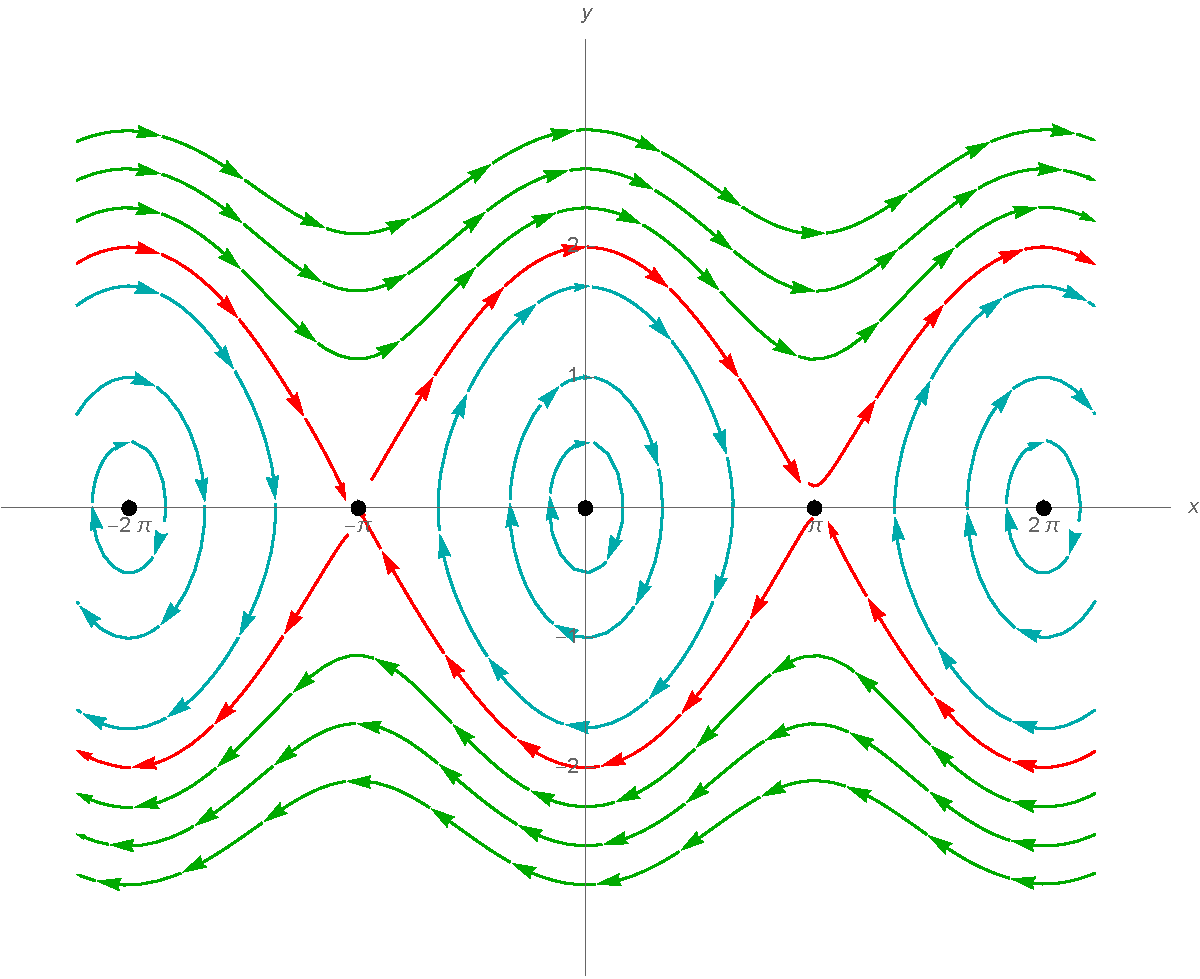
\includegraphics[width=.7\linewidth]{images/pendulum.pdf}
    \caption{Integral curves for the pendulum}
    \label{fig:pendulum}
\end{figure}

From these examples we already see that phase curves can consist of only one point. In such case they are called \emph{equilibrium} points.

\subsection{The conservation of energy}\label{sec:energy}

Let's see how general is the phenomenon described in the previous section.

\begin{tcolorbox}
    Given a mechanical system, the function $I = I(q, \dot q, t)$ of the coordinates, their time derivatives and (possibly) time, is called the \emph{(first) integral}, or \emph{constant of motion} or \emph{conserved quantity}, if the total derivative of the function $I$ is zero:
    \begin{equation}\label{eq:firstintegralD}
        \frac{\d}{\d t}I =
            \frac{\partial I}{\partial q^i} \dot q^i + 
            \frac{\partial I}{\partial \dot q^i} \ddot q^i +
            \frac{\partial I}{\partial t}
            = 0.
    \end{equation}
\end{tcolorbox}

In other words, if the function $I$ remains constant along the paths followed by the system:
\begin{equation}
    I(q(t),\dot q(t), t) = \mathrm{const}.
\end{equation}

\begin{theorem}\label{thm:conservationEnergy}
If the lagrangian of the mechanical system does not explicitly depend on time, $L = L(q, \dot q)$, then the \emph{energy} of the system
\begin{equation}\label{eq:energy1}
    E(q,\dot q) = p_i \dot q^i - L,\qquad p_i := \frac{\partial L}{\partial \dot q^i}
\end{equation}
is conserved.
\end{theorem}
\begin{proof}
    Using the Euler-Lagrange equation, we have
    \begin{equation}
        \frac{\d}{\d t} L
        = \frac{\partial L}{\partial q^i} \dot q^i + \frac{\partial L}{\partial \dot q^i} \ddot q^i
        \overset{\text{(EL)}}{=} \dot q^i \frac{\d}{\d t} \frac{\partial L}{\partial \dot q^i} + \frac{\partial L}{\partial \dot q^i} \ddot q^i
        = \frac{\d}{\d t}\left(\frac{\partial L}{\partial \dot q^i} \dot q^i\right),
    \end{equation}
    that is,
    \begin{equation}
        \frac{\d}{\d t}\left(\frac{\partial L}{\partial \dot q^i} \dot q^i - L\right) = 0.
    \end{equation}
\end{proof}

\begin{example}\label{ex:natlagham}
    Let's consider $N$ point particles in physical space with natural lagrangian $L = T - U$ as in \eqref{eq:mechlag}.
    Then,
    \begin{equation}
        \bp_k = \frac{\partial L}{\partial \dot\bx_k} = m_k \dot \bx_k,
    \end{equation}
    and therefore
    \begin{equation}
        \sum_{k=1}^{N} \lag\bp_k, \dot\bx_k\rag = \sum_{k=1}^{N} m_k \|\dot\bx\|^2 = 2 T
    \end{equation}
    which implies that the energy of the mechanical system is
    \begin{equation}\label{eq:energyFromL}
        E = 2T - T + U = T + U.
    \end{equation}
    Defining the kinetic momentum $\bp_k := m_k \dot \bx_k$, we get $E = H(q,p) := \frac{1}{m_k}\|\bp_k\|^2 + U$, the sum of kinetic and potential energies, as in \eqref{eq:energyKepler} and Theorem \ref{thm:ham1}.
\end{example}

\begin{remark}
    This is probably a good point to discuss the question: why does nature want to minimize the action? And why the lagrangian is of the form \eqref{eq:mechlag}?

    Theorem~\ref{thm:conservationEnergy} tells us that the total energy is conserved, and \eqref{eq:energyFromL} tells us that for closed systems this implies that the energy is transferred back and forth between the kinetic and the potential components.
    We saw towards the end of Section~\ref{sec:dynamicspps} that while the kinetic energy measures how much the system is moving around, the potential energy measures the capacity of the system to change: its name can be intended as `potential' in the sense of yet unexpressed possibilities.

    Looking at the lagrangian itself, we see that it is minimal when the potential energy is large and maximal when the kinetic energy is large.
    So, the lagrangian measures in some sense how `active' a system is: the higher the kinetic energy the more active a system is, and the higher the potential energy the less active the system.
    %
    The principle of least action tells us that nature is lazy: she likes to find a compromise that minimizes its activity over time, i.e. its total action.

    You can read a nice historical account on how scientists came up with the principle of least action in \cite{lectures:baez}.
\end{remark}

\begin{exercise}
    \begin{enumerate}
        \item Derive formula \eqref{eq:energyFromL} for a natural lagrangian on a riemannian manifold $(M,g)$.
        \item Given any lagrangian of the form $L = L(q, \dot q)$ on $TM$, show that the definition of energy \eqref{eq:energy1} does not depend on the choice of local coordinates on $M$. (Hint: look at Exercise~\ref{exe:coordinatesInd}).
        \item Consider the following free lagrangian on a riemannian manifold $(M, g)$:
        \begin{equation}
            L = \frac12 g_{ij}(q)\dot q^i \dot q^j.
        \end{equation}
        We have already seen in Exercise \ref{exe:geodesic1} that the solutions of the Euler-Lagrange equations are geodesic curves.
        Show that geodesic curves have constant speed, i.e. $(\dot q, \dot q) = \mathrm{const}$.
        %\item Consider a time-dependent lagrangian $L = L(q,\dot q, t)$. Show that $\frac{\d}{\d t} E = \frac{\partial E}{\partial t}$.
    \end{enumerate}
\end{exercise}


% Exercise: H\'enon-Heiles 1964
% Prove that H is a conserved quantity
% Energy hypersurface is 3-sphere: R^3 + {\infty} and also union of two solid tori glued along the common boundary (2-torus)
% Seifert foliation of 3-sphere
% First question: in one deg of freedom everything is conservative, how about more degrees of freedom?

% Lecture: page 22, Chapter 2.5 Arnold on conservation of energy in 2 deg of freedom.

\subsection{Back to one degree of freedom, again}\label{sec:1deg-again}

As we observed in the previous sections, the conservation of energy has remarkable consequences for systems with one degree of freedom.
In this final section, we will investigate this into more details.

A general natural lagrangian for a system with one degree of freedom in isolation has the form
\begin{equation}
    L = \frac12 g(q)\dot q^2 - U(q).
\end{equation}
As one would hope, in cartesian coordinates $q = x$ we obtain the natural lagrangian $L = \frac{m \dot x^2}{2} - U(x)$.
In this case we can easily observe that Theorem \ref{thm:ham1} and Theorem \ref{thm:conservationEnergy} coincide.

As we have seen in Section~\ref{sec:bdf}, the conservation of energy,
\begin{equation}\label{eq:cenergy1}
    \frac{m \dot x^2}{2} + U(x) = E \in\R \mbox{ constant},
\end{equation}
allows us to explicitly describe phase curves, i.e., solutions of the equations of motion in the plane $(x, y := \dot x)$.
On each phase curve the value of the energy is constant, so the phase curve lies entirely in one energy level (the set of points $H(x,y)=E$).

More explicitly, we can use \eqref{eq:cenergy1} to integrate the equations of motion
\begin{equation}
    m \ddot x = - \frac{\d U(x)}{\d x}
\end{equation}
by quadrature, i.e., solving the equation as
\begin{equation}
    t_2 - t_1 = \frac m2 \int_{x_1}^{x_2} \frac{\d x}{\sqrt{E-U(x)}},
\end{equation}
and to reason about further properties of the solutions.

Given that the kinetic energy is always non-negative, $E \geq U(x)$, and thus, the point can move only in the intervals $U(x) \leq E$.
At the points $x^* = x^*(E)$ such that $U(x^*) = E$, we have $\dot x^* = 0$ and if the motion is bounded between two such points, say $x_1^*$ and $x_2^*$, then the motion has to be finite.
Furthermore, it must be an \emph{oscillatory} motion: the point particles move inside the potential well between the points $x_1^*$ and $x_2^*$.

Thanks to time reversibility, the time of travel between $x_1^*$ and $x_2^*$ is the same as the time to return from $x_2^*$ to $x_1^*$, therefore the period of oscillation is given by
\begin{equation}\label{eq:osc}
    T(E) = \sqrt{2m} \int_{x^*_1}^{x^*_2} \frac{\d x}{\sqrt{E-U(x)}}.
\end{equation}

A special subset of these finite motions is the one on the critical points of the force, i.e., the points $x^*$ such that 
\begin{equation}
    \frac{\partial U}{\partial x}(x^*) = 0.
\end{equation}
In this case, the phase curve is made of a single point on the $x$-axis: if we start with the initial conditions $x(0) = x^*$ and $\dot x(0) = 0$, the system will stay there forever. These points are called \emph{equilibrium points}.

Any other motion, not bounded by two points $x^*$, is going to be infinite (or semi-infinite).

See also \cite[Chapter 2.4]{book:arnold}, especially Figures 10, 11 and 12.

\begin{remark}
    Integral curves carry more information than what immediately meets the eye.
    Observe for example that there is a remarkable relation between the period of an oscillation and the area of the integral curve $H(x,y) = E$:
    if $A$ is the area enclosed by the integral curve, then the period $T$ can be obtained as
    \begin{equation}
        T = \frac{\d A}{\d E}.
    \end{equation}
    
    We will see this in more generality once we deal with action--angle coordinates, but let's sketch the proof in this case.
    
    From $H(x,y) = E$ we get $y = \pm \sqrt{2(U(x) - E)}$. Say that the curve intercepts the $x$-axis at the two return points $x_m < x_M$, then the area inside the curve, is given by
    \begin{equation}
        A = 2\int_{x_m}^{x_M}\sqrt{2(E - U(x))} \d x.
    \end{equation}
    As we saw above, the period can be computed as
    \begin{equation}
        T = 2\int_{x_m}^{x_M} \frac{\d x}{\sqrt{2(E - U(x))}}.
    \end{equation}
    
    With the above in mind, the result follows by taking the derivative of $A$ with respect to $E$.
\end{remark}

\begin{example}\label{ex:small-osc}
    Looking back at Example \ref{ex:sprPen}, the lagrangian of a pendulum of length $l$ and mass $m$ is given by
    \begin{equation}
        L = \frac{ml^2 \dot x^2}2 + mgl \cos x,
    \end{equation}
    thus $E = \frac{ml^2 \dot x^2}2 - mgl \cos x$.
    The motion is bounded for $|E| \leq mgl$. For any such motions, the angle of maximal oscillation corresponds to a solution of $U(x) = E$, thus is given by $E = -mgl \cos x^*$ for some $x^*$.
    Finally, \eqref{eq:osc} implies that the period of oscillation is
    \begin{equation}
        T(E) = 4 \sqrt{\frac l{2g}} \int_0^{x^*(E)} \frac{\d x}{\sqrt{\cos(x) - \cos(x^*(E))}},
    \end{equation}
    which, as we briefly discussed previously, does not depend on the mass of the pendulum, but only on its length!

    It is possible to use the previous formula to express the period of oscillation in terms of elliptic integrals
    \begin{equation}
        T = 4 \sqrt{\frac lg} K\left (\sin(x^*/2)\right), \quad
        K(k):= \int_0^{\pi/2} \frac{\d \theta}{\sqrt{1 - k^2\sin^2(\theta)}}.
    \end{equation}
    If the oscillations are small, $x^* = \epsilon \ll 1$, this form allows for an immediate expansion of the form
    \begin{equation}\label{eq:smallosc-preview}
        T_\mathrm{p} = 2\pi \sqrt{\frac lg} \left(1 + \frac{\epsilon^2}{16} + O(\epsilon^4)\right).
    \end{equation}

    Equation \eqref{eq:smallosc-preview} implies that for \emph{small oscillations}, the period of oscillation does not depend on the amplitude (and thus on the energy $E$). Which is the same result that you get by approximating the potential for small $x$ by a second order polynomial
    \begin{equation}
        U(x) = -mgl \cos x = C + \frac{mgl}2 x^2 + O(x^4)
    \end{equation}
    and study the corresponding system.

    Indeed, ignoring the constant $C$ for conciseness, one finds the harmonic oscillator lagrangian
    \begin{equation}
        L_{\mathrm{ho}} = \frac{ml^2 \dot x^2}{2} - \frac{mgl x^2}{2},
    \end{equation}
    which we already solved in Example \ref{ex:sprPen}.
    In this specific case $\omega = \sqrt{g/l}$ and the corresponding period of oscillation is
    \begin{equation}
        T_{\mathrm{ho}} = \frac{2\pi}\omega = 2\pi \sqrt{\frac lg} \sim T_\mathrm{p}.
    \end{equation}

    This is an example of a more general phenomenon that we will discuss soon in details.
\end{example}

Before concluding this chapter let's discuss a final example where we can make use of non cartesian generalized coordinates.

\begin{example}[Double pendulum]\label{ex:2pendulum}
    A double pendulum consists of two point particles of masses $m_1$ and $m_2$, connected by massless rods of lengths $l_1$ and $l_2$. The first pendulum is attached to the ceiling by a fixed pivot while the second one is attached to the point particle of the first pendulum.

    Denote $x_1$ and $x_2$ the angles that each of the pendulums make with respect to the corresponding vertical, oriented counterclockwise: a value of $0$ means that the pendulum is vertical with the mass lying below the pivot.
    
    The lagrangian $L_1 = T_1 - U_1$ of the first particle is the same as for a simple pendulum:
    \begin{equation}
        T_1 = \frac{m_1 l_1^2 \dot x_1^2}2,
        \quad\mbox{and}\quad
        U_1(x_1) = -m_1 g l_1 \cos x_1,
    \end{equation}
    where $g$ is the usual gravitational acceleration.

    The lagrangian corresponding to the second particle is a bit more involved. We start by considering the position of the second particle in the $(\chi,\eta)$-plane in which the pendulum swings, centered at the pivot of the first pendulum and with $\eta$ positive in the downward direction:
    \begin{equation}
        \chi = l_1\sin x_1 + l_2\sin x_2,
        \quad\mbox{and}\quad
        \eta = l_1\cos x_1 + l_2\cos x_2.
    \end{equation}
    We can substitute these values into the kinetic energy for the second particle in cartesian coordinates $(\chi,\eta)$ to get
    \begin{equation}
        T_2 = \frac {m_2 (\dot\chi^2 + \dot\eta^2)}2
            = \frac {m_2}2 \left(
                l_1^2 \dot x_1^2 + l_2^2 \dot x_2^2
                + 2l_1l_2 \cos(x_1 -x_2)\dot x_1 \dot x_2
                \right),
    \end{equation}
    while the potential energy is given by
    \begin{equation}
        U_2 = -m_2 g \eta = -m_2g (l_1\cos x_1 + l_2\cos x_2).
    \end{equation}
    The full lagrangian is then given by
    \begin{align}
        L &= T_1 + T_2 - U_1 - U_2 \\
          &= \frac12 (m_1 + m_2)  l_1^2 \dot x_1^2
             + \frac 12 m_2 l_2^2 \dot x_2^2
             + m_2l_1l_2 \cos(x_1 -x_2)\dot x_1 \dot x_2 \\
             &\quad+ (m_1 + m_2) g l_1 \cos x_1
             + m_2gl_2\cos x_2.
    \end{align}

    We can now compute the equations of motion using Euler-Lagrange equations and try to solve them.
    The solutions are complicated and, in fact, after a certain energy threshold the motion is chaotic.
    You can have some fun looking at the daily simulations of the pendulum bot: \url{https://twitter.com/pendulum_bot}. 
    We will come back to this problem after discussing symmetries and small oscillations.
\end{example}

One final example, with two degrees of freedom, before jumping into variational principles.

\begin{example}[Lissajous Figures]\label{exa:lissajous}
Consider the system of independent harmonic oscillators
\begin{equation}
    \left\lbrace
    \begin{aligned}
        \ddot x_1 &= -x_1\\
        \ddot x_2 &= -\omega^2 x_2
    \end{aligned}
    \right..
\end{equation}
This can be explicitly solved: the equations are completely uncoupled and we know that the phase portrait of $x_1$ consists of circles while the phase portrait of $x_2$ consists of ellipses.

Together, the two equations define a 4 dimensional phase space. The curves in the phase space are combinations of closed curves in each phase space and describe a 2-torus.

We know from the previous part of this section that the energy of each oscillator is conserved, as well as the total energy:
\begin{equation}
    H_1 = \frac12\dot x_1^2 + \frac12 x_1^2, \quad
    H_2 = \frac12\dot x_2^2 + \frac12 \omega^2 x_2^2, \quad
    H = H_1 + H_2.
\end{equation}

The level curves $H=E$ describe a 3-sphere in $\mathbb{R}^4$, which are foliated by all the 2-tori of trajectories with energies that sum to $E$. For the more geometric inclined, you can look up ``H\'enon-Heiles model'', ``Seifert foliation of a three sphere'' or ``Hopf fibration'' to have a glimpse of some related fascinating topics.

\begin{figure}[ht]
    \centering
    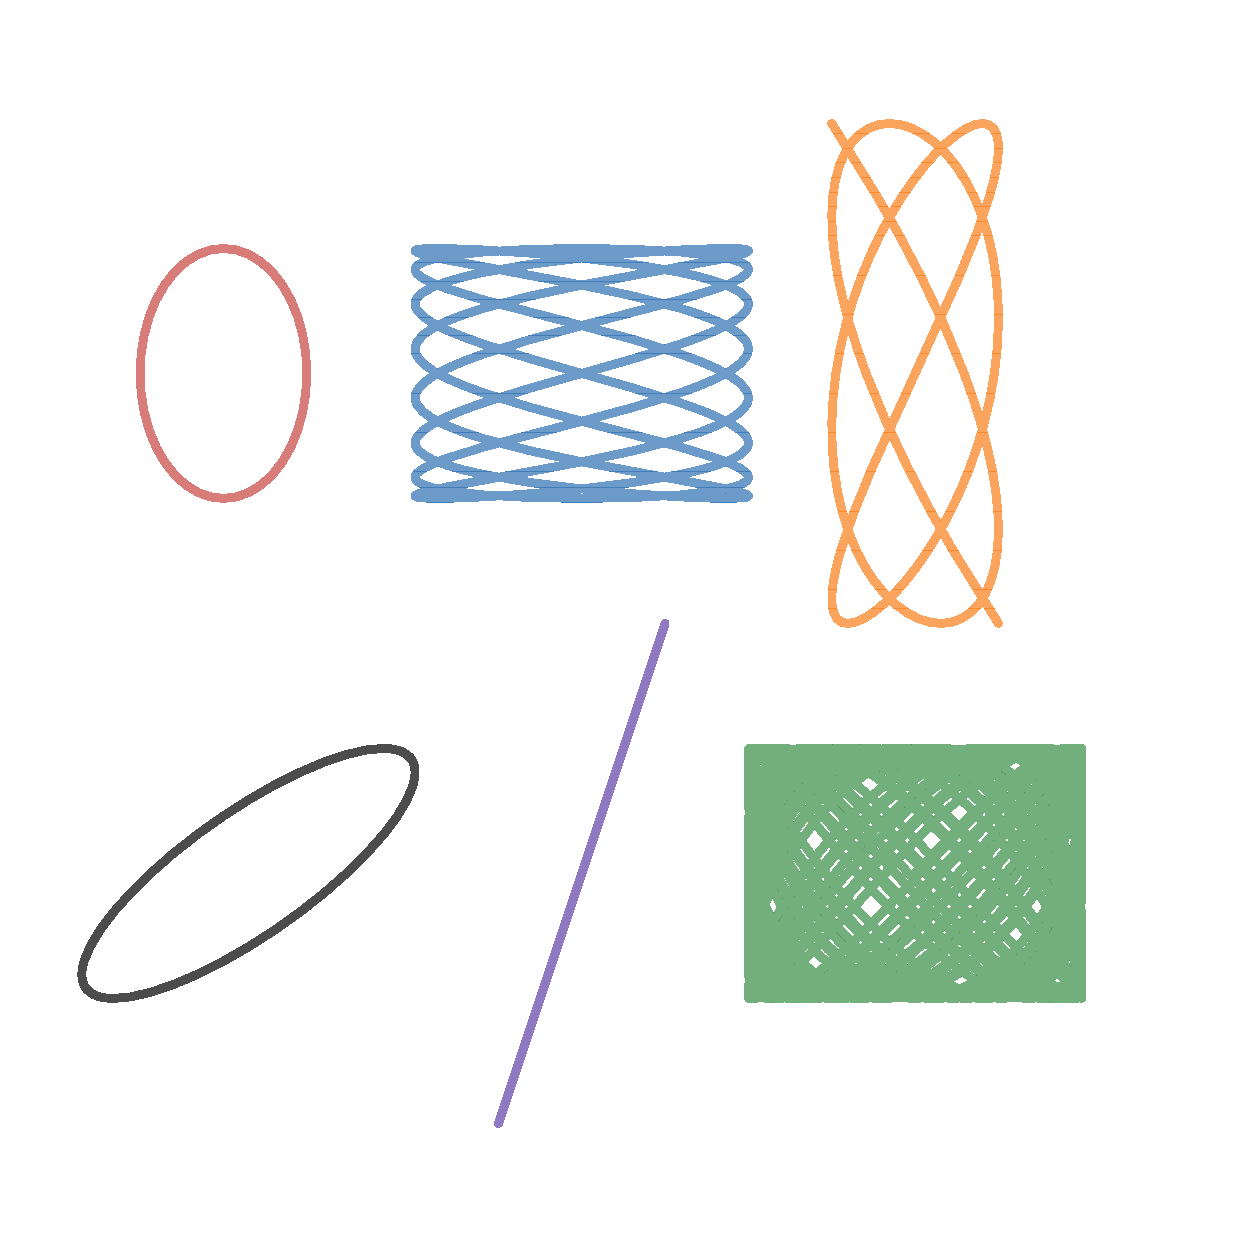
\includegraphics[width=.75\linewidth,trim={0 50pt 0 50pt},clip]{images/lissajous.pdf}
    \caption{Some casually selected Lissajous figures}
    \label{img:lissajous}
\end{figure}

On the configuration plane $(x_1, x_2)$, the motion that we observe is
\begin{equation}
    x(t) = \left( R_1 \cos(t + \phi_1),\, R_2 \cos(\omega t + \phi_2) \right).
\end{equation}
This is contained in a rectangle $[-R_1,R_1]\times[-R_2,R_2]$. When $\omega$ is irrational, the trajectory fills the rectangle, whereas they are closed curves inside the rectangle when it is rational. % not always closed, the top right example in the figure corresponds to a rational omega but it is not closed.
See also \cite[Exercise 6.34]{book:knauf} and \cite[Chapter 2.5, Example 2]{book:arnold}.
\end{example}

\begin{exercise}[Huygens problem]
    Determine the form of even potentials, $U(x) = U(-x)$, giving rise to \emph{isochronal} oscillations, i.e., whose period $T$ does not depend on $E$.

    Use your result to study the following problem.
    A point particle of mass $m$ moves without friction under the effect of a gravitational potential with uniform acceleration $g$ on the curve
    \begin{equation}
        \gamma(s) = (x(s), y(s)) \quad\mbox{such that}\quad
        \left\lbrace
        \begin{aligned}
            &\dot x(s) \neq 0, \\
            &x(-s) = -x(s), \; y(-s) = y(s)
        \end{aligned}
        \right.
    \end{equation}
    Find the lagrangian of the system and determine the shape of the curve so that the oscillations are isochronal.

    This is called Huygens problem: he was studying it to win a competition for the best maritime chronometer.

    Hint: use the natural parametrization for the curve: $\dot x^2 + \dot y^2 = 1$.
\end{exercise}

\begin{exercise}[The isoperimetric problem]
    In the $(x,y)$-plane in $P\subset \R^3$ you are given a curve $\gamma:[t_1,t_2]\to P$ connecting the points $(x_1, y_1, 0)$ and $(x_2, y_2, 0)$. Revolve this curve around the $x$-axis.
    
    For which curve does the corresponding surface of revolution have minimal area?
\end{exercise}

\begin{exercise}[The brachistochrone problem]
    Let $P$, $Q$ be two given points in the vertical $(x,y)$-plane, where $Q$ lies beneath $P$.
    A particle, subject to constant gravitational acceleration pointing downwards, moves from $P$ to $Q$, starting at rest.
    Determine the curve along which this motion takes the shortest time.
\end{exercise}


\chapter{Conservation Laws}

\section{Noether theorem}

In this section we go deeper into the appearance of conservation laws in the lagrangian formulation and, in particular, a beautiful and important theorem due to Emmy Noether relating conserved quantities to symmetries.

Later on, once we introduce hamiltonian mechanics, we will come back to the study of symmetries and conservation laws in a more sophisticated way.

We have already seen that, when the lagrangian is not explicitly time dependent, the total energy is a conserved quantity.
Can we expect more?

Let's make another example before entering into the gist of the matter.

\begin{example}[kinetic momentum]\label{ex:linearm}
    Consider a mechanical system with $n$ degrees of freedom described by the lagrangian $L=L(q,\dot q)$, $q=(q^1,\ldots,q^n)$.
    If there is $i$ such that $L$ does not depend on $q^i$, i.e.
    \begin{eqnarray}
        \frac{\partial L}{\partial q^i} = 0,
    \end{eqnarray}
    then the coordinate $q^i$ is said to be \emph{cyclic} and the kinetic momentum
    \begin{eqnarray}
        p_j := \frac{\partial L}{\partial\dot q^j}
    \end{eqnarray}
    is a conserved quantity.

    This is easily verified by using Euler-Lagrange equations:
    \begin{eqnarray}
        \frac{\d p_j}{\d t} =
        \frac{\d}{\d t} \left(\frac{\partial L}{\partial \dot q^j}\right)=
        \frac{\partial L}{\partial q^j} = 0.
    \end{eqnarray}
\end{example}

It seems that we can expect other conserved quantities. However, before being able to give a precise statement we need to introduce some preliminary concepts.

Let $M$ be a smooth manifold. A smooth map $\phi : M \to M$ is called \emph{diffeomorphism} if it is invertible and its inverse $\phi^{-1}$ is smooth. At each point $q\in M$ we can define the \emph{differential} of $\phi$, i.e. the linear map $\phi_*$ between tangent spaces (sometimes also denoted $\d\phi_q$)
\begin{equation}
    \phi_*: T_q M \to T_{\phi(q)} M,
    \quad \phi_* v = \phi_*(q) v := \frac{\d}{\d t} \phi(q + t v) \Big|_{t=0},
    \quad v\in T_q M.
\end{equation}
In local coordinates, the matrix of the linear map coincides with the Jacobian matrix
\begin{equation}
   \phi_*(q) = \d \phi_q = \left(\frac{\partial \phi^i(q)}{\partial q^j}\right)_{1\leq i,j\leq n}.
\end{equation}

The differential can be used to \emph{push} tangent vectors on $M$ \emph{forward} to tangent vectors on $\phi(M)$, which is why it is also called \emph{pushforward}.

\begin{tcolorbox}
    Let $L = L(q, \dot q)$, $(q, \dot q)\in TM$ be a lagrangian on the tangent bundle of a smooth manifold $M$. From now on, we will denote with $(M, L)$ the mechanical system described by such lagrangians $L$ on the configuration space $M$. 
\end{tcolorbox}

A diffeomorphism $\Phi: M \to M$ is called a \emph{symmetry} of the mechanical system $(M,L)$ if $L$ is invariant with respect to $\Phi$, i.e.
\begin{equation}\label{eq:symmetry}
    L\left(\Phi(q), \Phi_*\dot q\right) = L(q,\dot q) \qquad \forall q\in M, \forall\dot q \in T_q M.
\end{equation}
Note that in \cite[Chapter 4]{book:arnold} terminology, the above definition would instead be that \emph{$(M,L)$ admits the mapping $\Phi$}.

A fundamental property of symmetries of mechanical systems is summarized by the following theorem.

\begin{theorem}
    Let $\Phi$ be the symmetry of a mechanical system. If $q(t)$ is a solution of the Euler-Lagrange equations, then $\Phi(q(t))$ satisfies the same equations.
\end{theorem}

The converse is generally not true: i.e. in general it is not true that if $\Phi$ maps solutions to solutions, then $\Phi$ is a symmetry.

We are almost there.
Before being able to introduce Noether theorem we need one last definition.

A one--parameter family of diffeomorphisms
\begin{equation}
    \Phi_s : M \to M
\end{equation}
is called \emph{one--parameter group of diffeomorphisms} if the following hold:
\begin{itemize}
    \item $\Phi_0 = \Id$;
    \item $\forall s, t \in \R, \quad \Phi_s(\Phi_t(q)) = \Phi_{s+t}(q)\quad \forall q\in M$.
\end{itemize}
Observe that these two properties give away the inverse of $\Phi_s$: $(\Phi_s)^{-1} = \Phi_{-s}$.

\begin{remark}
\emph{To any one--parameter group of diffeomorphism we can associate a smooth vector field $X : q\in M \mapsto X(q)\in T_qM$} by
\begin{equation}
    X(q) := \frac{\d}{\d s} \Phi_s(q) \Big|_{s=0}.
\end{equation}
This is clearly seen for small values of $|s|$, in which case the diffeomorphism $\Phi_s$ acts as
\begin{equation}\label{eq:infinitesimalSymmetryExp}
    q \mapsto \Phi_s(q) = q + s X(q) + O(s^2).
\end{equation}

Moreover, the inverse relation also holds: \emph{given a smooth vector field $X(q)$, we can reconstruct a one--parameter group of diffeomorphisms} (at least for sufficiently small values of $s$) as follows.
Let $Q(s, q)$ be the solution of the initial value problem
\begin{equation}\label{eq:NoetherCoords}
    \frac{\d Q}{\d s} = X(q), \quad Q(s, q)\Big|_{s=0} = q.
\end{equation}
Assume that there exist $\epsilon >0$ such that for all $|s|<\epsilon$ the solution $Q(s,q)$ exists for every $q\in M$.
Then, the map $\Phi_s:M\to M$ is defined for $|s|<\epsilon$ by 
\begin{equation}\label{eq:reconstructX}
    \Phi_s(q) := Q(s, q).
\end{equation}

\begin{exercise}
    Show that $\Phi_s$ as defined in \eqref{eq:reconstructX} is a one--parameter group of diffeomorphisms on $M$ for $s,t \in(-\epsilon,\epsilon)$ such that $|s + t| < \epsilon$.
\end{exercise}

For a more thorough account of these topics, and to understand how this relates to the concept of infinitesimal generators of group actions, refer to \cite[Chapters 9 and 20]{book:lee}.
\end{remark}

\begin{theorem}[Noether theorem]\label{thm:noether}
    Given a one--parameter group of symmetries $\Phi_s: M \to M$ of the mechanical system $(M,L)$, then there exists an integral of motion $I: TM \to \R$.
    In local coordinates $q$ on $M$, the integral $I$ takes the form
    \begin{equation}
        I(q,\dot q) := p_i X^i,
        \quad p_i(q, \dot q) := \frac{\partial L}{\partial \dot q^i},
        \quad X(q) := \frac{\d}{\d s} \Phi_s(q) \Big|_{s=0}.
    \end{equation}
\end{theorem}

Although I prefer the presentation of the proof in \cite[Chapter 20.B]{book:arnold}, I will give here one with a slightly different perspective.
\begin{proof}
    By definition, see \eqref{eq:firstintegralD}, $I$ is a first integral if it is constant on the phase curves.
    Let's compute its time derivative,
    \begin{align}
        \frac{\d}{\d t} I(q, \dot q)
          & = \frac{\d}{\d t} p_i(q, \dot q) X^i(q) \\
          &= \frac{\d p_i}{\d t} X^i + p_i \frac{\partial X^i}{\partial q^j} \dot q^j \\
          &= \left(\frac{\d}{\d t}\frac{\partial L}{\partial \dot q^i}\right) X^i + p_i \frac{\partial X^i}{\partial q^j} \dot q^j \\
          &= \frac{\partial L}{\partial q^i} X^i + p_i \frac{\partial X^i}{\partial q^j} \dot q^j. \label{eq:ntref1}
    \end{align}
    The last equality follows from the Euler-Lagrange equations.
    
    We are left to show that one of the equations appearing above is $0$, and we have not yet used that we have a one--parameter group of symmetries.
    Using the representation \eqref{eq:infinitesimalSymmetryExp}, we can rewrite the symmetry relation \eqref{eq:symmetry} as
    \begin{equation}\label{eq:invariance}
        L\left( q + s X(q), \dot q + s \frac{\partial X}{\partial q} \dot q\right) = L(q, \dot q) + O(s^2).
    \end{equation}
    Expanding the left hand side in series for small $s$, and simplifying the term $L(q, \dot q)$, the condition becomes
    \begin{equation}\label{eq:ntref2}
        \frac{\partial L}{\partial q^i} X^i + p_i \frac{\partial X^i}{\partial q^j} \dot q^j = 0.
    \end{equation}
    Which shows that \eqref{eq:ntref1} is $0$ and, thus, that $I$ is a first integral.
\end{proof}

\begin{example}[kinetic momentum - reprise]\label{exa:kmom}
    Let's revisit Example~\ref{ex:linearm}.
    For a cyclic coordinate $q^i$, the lagrangian is invariant with respect to the one--parameter group of translations along the $q^i$ direction:
    \begin{equation}
        \Phi_s(q^1, \ldots, q^i, \ldots, q^n) = (q^1, \ldots, q^i + s, \ldots, q^n).
    \end{equation}
    The corresponding vector field $X$ is constant: $X(q)^j = \delta^j_i$, $1$ in the $i$-th component, and zero everywhere else.
    By Noether theorem, the conserved quantity is
    \begin{equation}
        I(q,\dot q) = p_j X^j = p_j \delta^j_i = p_i,
    \end{equation}
    as expected.
\end{example}

\begin{remark}
    Noether theorem is a more general result related to symmetries in classical field theories than what we presented here.
    The proof of the more general Noether theorem is obtained by reducing the system to a system with one cyclic variable.
    This can be done by locally rectifying the vector field $X$ on $M$ and observing that, by Exercise~\ref{exe:coordinatesInd}, the sum $p_i X^i$ does not depend on the choice of coordinates on $M$.
\end{remark}

\begin{exercise}
    Assume that the one--parameter group of diffeomorphisms $\Phi_s$ is \emph{not} a symmetry for $(M,L)$ in the sense of our definition, but \emph{preserves the action $S$ associated to the lagrangian}.
    In that case, the invariance condition \eqref{eq:invariance} holds only up to total derivatives \cite[Chapter 4.20]{book:gelfand}, i.e. there is a function $f(q)$ on $M$ such that
    \begin{equation}
        L\left( q + s X(q), \dot q + s \frac{\partial X}{\partial q} \dot q\right)
        = L(q, \dot q) + s \frac{\d}{\d t}f(q) + O(s^2).
    \end{equation}
    Show that in this case the first integral of the system would be
    \begin{equation}
        \tilde I(q, \dot q) = p_i X^i - f(q).
    \end{equation}
\end{exercise}

\begin{remark}
    There are also discrete symmetries in nature which don't depend on a continuous parameter. The so-called parity, for example, is the invariance under reflection, $\bx \mapsto -\bx$.
    These types of symmetries give rise to conservation laws in quantum physics but \emph{not} in classical physics.
\end{remark}

Let's now look at more and less immediate consequences of our discovery, starting from some of the invariants that we have already seen.

\subsection{Homogeneity of space: total momentum}

Consider a system of $N$ particles with lagrangian \eqref{eq:mechlag},
\begin{equation}
    L = \frac21 \sum_{k=1}^N m_k \dot \bx_k^2 - U(\bx_1, \ldots, \bx_N),
\end{equation}
which is invariant with respect to translations
\begin{equation}
    \Phi_s(\bx_1, \ldots, \bx_N) := (\bx_1 + s \hat \bx,\ldots, \bx_N + s \hat \bx),
\end{equation}
for any direction $\hat\bx$, $|\hat\bx|=1$ and all $s\in\R$. I.e.
\begin{equation}
    L(\bx_1, \ldots, \bx_N, \dot \bx, t) = L(\bx_1 + s \hat\bx, \ldots, \bx_N + s \hat\bx, \dot \bx, t),
\end{equation}
which is the statement that space is homogeneous and a translation of the system in some direction $\hat\bx$ does nothing to the equations of motion. These translations are elements of the Galilean group that we met in Chapter~\ref{sec:varpri}.

We call \emph{total momentum} the vectorial quantity
\begin{equation}
    \bm{P} = \sum_{k=1}^N m_k \dot \bx_k = \sum_{k=1}^N p_k.
\end{equation}

As we saw in Example~\ref{exa:kmom}, Noether theorem implies that for any $\hat\bx$, the projection of the total impulse on the direction $\hat\bx$, which is
\begin{equation}
    (\bm{P}, \hat\bx) = \sum_{k=1}^N (p_k, \hat\bx),
\end{equation}
is a conserved quantity.
Since $\hat\bx$ is arbitrary, this means that also $\bm{P}$ is conserved.

This should be intuitively clear: one point in space is much the same as any other. So why would a system of particles speed up to get somewhere else, when its current position is just as good? This manifests itself as conservation of momentum.

This fact can be also interpreted in the following way: the sum of all forces acting on the point particles in the closed system is zero, i.e. Newton's third law $\sum_k \bm{F}_k = 0$. Which, by now, you may have also figured out by solving Exercise \ref{ex:N3l1}.

\begin{example}[The baricenter]
    Consider the galilean transformation $t \mapsto t$, $\bx \mapsto \bx' + \bm{v}t$.
    The total momentum $\bm{P}$ transforms as
    \begin{equation}
        \bm{P} = \bm{P}' + \bm{v}  \sum_{k=1}^N m_k.
    \end{equation}
    If the total momentum is zero with respect to some reference frame, we say that the system is \emph{stationary} in the reference frame. For a closed system, it is always possible to find an inertial frame of reference, called co-moving frame, in which the system becomes stationary. The speed of such special reference frame,
    \begin{equation}
        \bm{v_T} = \frac{\bm{P}}{\sum_{k=1}^N m_k}
               = \frac{\sum_{k=1}^N m_k \dot \bx_k}{\sum_{k=1}^N m_k},
    \end{equation}
    can be thought of as the total speed of the mechanical system.
    A rewriting of the formula above gives
    \begin{equation}
        \bm{P} = M \bm{v_T}, \quad M:= \sum_{k=1}^N m_k.
    \end{equation}
    In other words, the total momentum of the system is equal to the product of the total mass and the total speed of the system.
    In view of this, we could reinterpret the total speed of the system, seen as a whole, as the speed of a virtual point particle with position
    \begin{equation}
        \bm{X} = \frac{\sum_{k=1}^N m_k \bx_k}{M}.
    \end{equation}
    This special point is called \emph{barycenter} of the system.
    \medskip

    Calling \emph{internal energy $E_i$} of a system its total energy in the co-moving frame, the energy of the system with respect to another inertial reference frame is given by
    \begin{equation}
        E = E_i + \frac{M |\bm{v_T}|^2}{2}, \quad M= \sum_{k=1}^N m_k.
    \end{equation}
\end{example}

\begin{exercise}
    Consider, as in Example~\ref{exa:magnetic} and Exercise~\ref{exe:magnetic}, a closed system of charged point particles in the presence of a uniform constant magnetic field $\bm{B}$. Define
    \begin{equation}
        \tilde{\bm{P}} := \bm{P} + \frac{e}c \bm{B}\times \bm{X},
    \end{equation}
    where $\bm{P}$ is the total momentum of the system when $\bm{B} = 0$ and $\bm{X}$ is the barycenter.
    Show that for such system, $\tilde{\bm{P}}$ is a conserved quantity.
\end{exercise}

\subsection{Isotropy of space: angular momentum}\label{sec:angm}

The isotropy of space is the statement that a closed system is invariant under rotations around a fixed axis. To work out the corresponding conserved quantities one can work directly with the infinitesimal form of the rotations.

Let's first look at the invariants related to isotropy:
rotations around an axis in $\R^3$ are identifiable with orthogonal transformation $A\in SO(3)$, the special orthogonal group -- orthogonal matrices $A^TA = Id$ with determinant $1$.

For future reference, it is worth recalling in more generality the structure of these transformations. We will do it briefly, for more details on the special orthogonal groups and their relation to rotations and vector products, you can refer to \cite{book:marsdenratiu}. 

Consider, for some small $\epsilon > 0$, a family of orthogonal matrices around the identity
\begin{equation}\label{eq:familyson}
    A(s) \in SO(n), \quad A(0) = \Id, \quad |s| < \epsilon.
\end{equation}
If we look at $SO(n)$ as the smooth manifold in the space $M^{n\times n}$ of $n\times n$ matrices defined by the equations
\begin{equation}
    A^T A = \Id,\quad \det A = 1,
\end{equation}
then its tangent space over the identity is
\begin{equation}
    T_{\Id} SO(n) = \big\{X\in M^{n\times n}\mid X^T = -X\big\},
\end{equation}
the space of antisymmetric $n\times n$ matrices.

This is a consequence of the following proposition.
\begin{proposition}
    Let $A(s)$ be a one--parameter family of orthogonal matrices of the form \eqref{eq:familyson}.
    Then,
    \begin{equation}\label{eq:form}
        A(s) = \Id + sX + O(s^2), \quad A^T(s)A(s) = \Id
    \end{equation}
    and the matrix $X$ is antisymmetric ($X^T = - X$).
    Moreover, the converse relation also holds: given an antisymmetric matrix $X$, there is a one--parameter family of orthogonal matrices $A(s)$ of the form \eqref{eq:form}.
\end{proposition}
\begin{proof}
    The local form \eqref{eq:form} is immediately obtained by expanding the family of matrices for small $s$ and using the orthogonality condition $A^TA = \Id$.
    This in turns implies
    \begin{align}
        \Id &= A^T(s) A(s) \\
        &= \left(\Id + sX + O(s^2)\right)^T\left(\Id + sX + O(s^2)\right) \\
        &= \Id + s(X^T + X) + O(s^2),
    \end{align}
    which can hold only if $X^T + X =0$.

    Conversely, given $X$ antisymmetric, the one--parameter family
    \begin{equation}
        A(s) := e^{sX} = \Id + s X + \frac{s^2}{2!} X^2 + \cdots
    \end{equation}
    is orthogonal for all $s$ by definition:
    \begin{equation}
        A^T(s)A(s) = e^{sX^T}e^{sX} = e^{-sX} e^{sX} = \Id.
    \end{equation}
\end{proof}

\begin{exercise}[Euler theorem]\label{exe:rotations}
    Given an antisymmetric matrix 
    \begin{equation}
        X = (X_{ij})_{1\leq i,j\leq 3},
    \end{equation}
    show that, for sufficiently small $s\in\R$ and modulo higher order corrections, the transformation
    \begin{equation}
        \bx \mapsto \bx + s X \bx + O(s^2)
    \end{equation}
    is the rotation around the axis through the origin and parallel to $\bm{N}
     = (X_{32}, X_{13}, X_{21})$ of angle $\delta\phi = s|\bm{N}|$.
    For an hint, see \cite[Chpater 26.D]{book:arnold}.
\end{exercise}

In view of Exercise~\ref{exe:rotations}, Noether theorem tells us that the conserved quantity for a single particle system would be
\begin{equation}
    I = (\bp, (X\bx)) = (\bp, [\bm{N}, \bx]) = (\bm{N}, [\bx, \bp]),
\end{equation}
where for the second equality we used the relation between $3\times3$ skew-symmetric matrices and vector products, and for the last we used the cyclicity of the vector product.
The quantity
\begin{equation}
    \bm{M} = [\bx, \bp]
\end{equation}
is called \emph{angular momentum}.

\begin{theorem}
If a closed system of $N$ particles is invariant with respect to rotations, then the components of its \emph{total angular momentum}
\end{theorem}
\begin{equation}
    \bm{M} = \sum_{k=1}^N [\bx_k, \bp_k]
\end{equation}
are conserved quantities.
\begin{proof}
On the configuration space $\R^{3N}$ we consider the simultaneous rotation of all the point particles
\begin{equation}
(\bx_1,\ldots,\bx_N) \mapsto 
(\bx_1,\ldots,\bx_N) +
s (X\bx_1,\ldots,X\bx_N) + O(s^2).
\end{equation}
This is associated to the vector field $(\bx_1,\ldots,\bx_N) \mapsto (X\bx_1,\ldots,X\bx_N)$ and, by Noether theorem, to the first integral
\begin{equation}
    I_X = \sum_{k=1}^N (\bp_k, X\bx_k).
\end{equation}
As mentioned above, an antisymmetric matrix $X$ acts as the exterior product with a vector $\bm{X}$, and therefore
\begin{align}
    I_X &= \sum_{k=1}^N (\bp_k, [\bm{X},\bx_k]) \\
    &= \sum_{k=1}^N (\bm{X},[\bx_k, \bp_k]) \\
    &= (\bm{X}, \sum_{k=1}^N [\bx_k, \bp_k]) \\
    &= (\bm{X},\bm{M}).
\end{align}

The claim follows from the arbitrariness of $\bm{X}$.
\end{proof}

\begin{example}
    Consider a natural lagrangian \eqref{eq:mechlag} with an \emph{axial symmetry}, i.e. whose potential is invariant by simultaneous rotations around a fixed axis.
    For convenience let's say that such axis corresponds to the $z$ axis.
    Looking back at the proof above, we can infer that the conserved quantity will not be the full total momentum $\bm{M} = (M_x, M_y, M_z)$ but instead only its $z$ component:
    \begin{equation}
        M_z = \sum_{k=1}^N m_k\left(x_k \dot y_k - y_k \dot x_k\right) =
        \sum_{k=1}^N m_k r_k^2 \dot \phi_k.
    \end{equation}
    In the last expression we used the cylindrical coordinates $(r, \phi, z)$ to emphasize that the angular momentum is the analogue of the kinetic momentum but involving an angular velocity.

    Also, you can see that the angular momentum depends quadratically on the distance from the rotational axis. Its conservation means that if a point particle is moving closer to the symmetry axis, it needs to spin faster and faster.
\end{example}

\subsection{Homogeneity of time: the energy}

We discussed homogeneity of space and isotropy, and discovered that they are related to the conservation of different types of momentum.
One could now ask, what about homogeneity of time?

Homogeneity of time means that $L$ is invariant with respect to the transformation $t\mapsto t+s$, which in turn means $\frac{\partial L}{\partial t} = 0$. We already saw in Section~\ref{sec:energy} that for natural lagrangians this corresponds to conservation of energy! In other words, Time is to Energy as Space is to Momentum.

If you have taken a course on special relativity, you have probably seen that the combination of energy and $3$-momentum forms a $4$-vector which rotates under space-time transformations. You don't have to be Einstein to make the connection: the link between energy-momentum and time-space exists also in Newtonian mechanics.

\subsection{Scale invariance: Kepler's third law}

We have mentioned in Remark~\ref{rmk:manylagrangians} that the two lagrangians $L$ and $\alpha L$, $\alpha\neq0$, give rise to the same equations of motion.
This does not look like a symmetry in our sense, but it is worth investigating its meaning in light of what we have seen so far.

\begin{theorem}
    Let $L$ be a natural lagrangian $L=T-U$ as in \eqref{eq:mechlag} whose potential is a homogeneous function of degree $k$:
    \begin{equation}
        U(\lambda\bx_1, \ldots, \lambda\bx_N) = \lambda^k U(\bx_1, \ldots, \bx_N)
        \qquad\forall \lambda>0.
    \end{equation}
    Then the equations of motion are scale invariant with respect to the transformation
    \begin{equation}
        t \mapsto \lambda^{1-\frac{k}2} t, \qquad
        \bx_k \mapsto \lambda\bx_k \quad k=1,\ldots,n.
    \end{equation}
\end{theorem}
\begin{proof}
    The transformation
    \begin{equation}
        t \mapsto \mu t, \qquad
        \bx_k \mapsto \lambda\bx_k \quad k=1,\ldots,n,
    \end{equation}
    dilates the speeds as
    \begin{equation}
        \frac{\d}{\d t} \bx_k \mapsto \frac{\lambda}{\mu} \frac{\d}{\d t}\bx_k.
    \end{equation}
    Therefore
    \begin{equation}
        T \mapsto \frac{\lambda^2}{\mu^2} T, \qquad U \mapsto \lambda^k U.
    \end{equation}
    For $\mu = \lambda^{1-\frac{k}2}$ we have
    \begin{equation}
        L \mapsto \lambda^k T - \lambda^k U = \lambda^k L
    \end{equation}
    and thus the two lagrangian have the same equations of motion.
\end{proof}

\begin{example}[Harmonic oscillator]
    The potential of the harmonic oscillator
    \begin{equation}
        L = \frac{\dot x^2}2 - \omega^2 x^2
    \end{equation}
    is homogeneous of degree $2$. In this case $1-\frac k2 = 0$ so the period of oscillation does not depend on the amplitude of the oscillation, as we had already seen in a previous example.
\end{example}

\begin{example}[Kepler's third law]
    Recall Kepler's problem lagrangian from Examples~\ref{ex:Kepler0} and~\ref{ex:kepler1}:
    \begin{equation}
        L = \frac{m \dot \bx^2}{2} + \frac{\alpha}{\|\bx\|}, \quad \alpha >0.
    \end{equation}
    In this case, the potential is homogeneous of degree $-1$. Therefore $1-k/2 = 3/2$, which means that the planet orbit is invariant with respect to the transformations
    \begin{equation}
        \bx \mapsto \lambda^2 \bx, \qquad t \mapsto \lambda^3 t.
    \end{equation}

    This should remind you of \emph{Kepler's third law}: the square of the orbital period of a planet is directly proportional to the cube of the semi--major axis of its orbit, in symbols $\frac{T^2}{X^3} \sim \mathrm{const}$.
\end{example}

\section{The spherical pendulum}
Let's come back to the spherical pendulum, introduced in Example~\ref{ex:sphericalP}.
Assume it moves in the presence of constant gravitational acceleration $g$ pointing downwards.
It's an exercise in trigonometry to see that the lagrangian in spherical coordinates takes the form
\begin{equation}
    L = \frac m2 l^2 \left(\dot \theta^2 + \dot \phi^2 \sin^2\theta\right) + mgl \cos \theta.
\end{equation}

We can immediately see that $\phi$ is a cyclic coordinate, as such the corresponding kinetic momentum
\begin{equation}\label{eq:spI}
    I = \frac{\partial L}{\partial \dot\phi} = m l^2 \dot\phi\sin^2 \theta
\end{equation}
is a constant of motion.
With our choice coordinates, $I$ corresponds to the component of the angular momentum in the $\phi$ direction. We can now use \eqref{eq:spI} to replace all the appearances of $\dot\phi$ with
\begin{equation}
    \dot\phi = \frac{I}{ml^2 \sin^2\theta}.
\end{equation}

Computing the remaining equation of motion for $\theta$, we get
\begin{equation}
    ml^2 \ddot \theta = ml^2 \dot\phi^2\sin\theta\cos\theta - mgl \sin\theta = -ml^2\frac{\partial V_{\mathrm{eff}}}{\partial \theta}
\end{equation}
where
\begin{equation}
    V_{\mathrm{eff}} = -\frac{g}l\cos\theta + \frac{I^2}{2m^2l^4}\frac1{\sin^2\theta}.
\end{equation}

\begin{remark}
    Be careful here: Euler-Lagrange equations are derived under the assumption that the coordinates are independent. If you replace the quantity $I$ in the lagrangian itself, you will get an incorrect result!    
\end{remark}

We are left with one-degree of freedom in $\theta$, thus we can integrate by quadrature using the energy.
Indeed, the conservation of energy translates into
\begin{equation}
    E = \frac{\dot \theta^2}2 + V_{\mathrm{eff}}(\theta),
\end{equation}
where $E>\min_\theta V_{\mathrm{eff}}(\theta)$ is a constant, and therefore
\begin{equation}\label{eq:sptheta}
    t - t_0 = \frac1{\sqrt2}\int\frac{\d \theta}{\sqrt{E - V_{\mathrm{eff}}(\theta)}}
\end{equation}

Thanks to \eqref{eq:spI}, we can use \eqref{eq:sptheta} to solve for $\phi$:
\begin{equation}
    \phi = \int \frac{I}{ml^2} \frac1{\sin^2\theta} \;\d t
    = \frac{I}{\sqrt{2} m l^2}  \int \frac1{\sin^2\theta} \frac{1}{\sqrt{E - V_{\mathrm{eff}}(\theta)}}\; \d \theta
\end{equation}

Close to a minimum of the effective potential $V_{\mathrm{eff}}$, we have a bounded oscillatory motion in $\theta$ while the constant sign of $\dot\phi$ implies that the particle keeps spinning with various degrees of acceleration in the $\phi$ direction.

At a minimum $\theta_0$ of the effective potential, which occurs by a careful balancing of the energy and the angular momentum, we have a stable orbit.
Looking at small oscillations around this point as we did for the simple pendulum, one can prove that small oscillations about $\theta = \theta_0$ have a frequency $\omega^2 = \frac{\partial^2 V_{\mathrm{eff}}(\theta_0)}{\partial\theta^2}$.

\begin{exercise}
    Use the phase portrait to describe the behavior of $\theta(t)$, and the motion of the pendulum. Make sure to use the correct intervals of definition of $\phi$ and $\theta$.
\end{exercise}

As you can see, the existence of two integral of motion allowed us to practically solve the equations of motion and describe many details of the behavior of the system.

This is a far more general statement that we will see again at work for the Kepler's problem and for motions in central potentials, and that, once we introduce hamiltonian systems, will be at the core of integrable systems and perturbation theory.


\section{Intermezzo: small oscillations}\label{sec:soc}
We have already seen a few cases in which, by a small perturbation near a stable equilibrium, we could describe with various degrees of accuracy the behavior of mechanical systems in terms of the motion of an harmonic oscillator.

In this section we will see that this phenomenon is much more general (and useful) by showing that the motion of systems close to equilibrium is described by a number of \emph{decoupled simple harmonic oscillators}, each ringing at a different frequency.

Let's revisit what we saw in Sections~\ref{sec:bdf} and \ref{sec:1deg-again} in slightly more generality and in a more organic way. Let's consider the Newton equation for a closed system with one degree of freedom in the presence of conservative forces, i.e. an equation like \eqref{eq:oscillator}:
\begin{equation}
    \ddot x = F(x).
\end{equation}

As we saw in Example~\ref{ex:small-osc}, it makes sense to ask ourselves what does the motion look like around an equilibrium point $x^*$, i.e. a point such that $F(x^*) = 0$.
To analyze this in more details, we \emph{linearize} the equation. 
Let $x(t)$ be a small perturbation around $x^*$. For convenience,
\begin{equation}
    x(t) = x^* + \gamma(t),
\end{equation}
where $\gamma$ is small so that we can expand $F$ in Taylor series around $x^*$, getting
\begin{equation}
    \ddot \gamma = \frac{\d F}{\d x}(x^*)\gamma + O(\gamma^2).
\end{equation}
Neglecting the higher order terms, we can see that there are three possibilities.
\begin{itemize}
    \item If $\frac{\d F}{\d x}(x^*) < 0$, the system behaves like a spring \eqref{eq:spring} with $\omega_0^2 = -\frac{\d F}{\d x}(x^*)$. The general solution \eqref{eq:springsol} tells us that the system undergoes stable oscillations around $x^*$ with frequency $\omega_0$ (and period $\tau_0 = 2\pi/\omega_0$).
    \item If, on the other hand, $\frac{\d F}{\d x}(x^*) > 0$, the force is pushing the system away from the equilibrium: the solution is of the form $\gamma(t) = C_+ e^{\lambda t} + C_- e^{-\lambda t}$, for some integration constants $C_+$ and $C_-$ and with $\omega_0^2 = \frac{\d F}{\d x}(x^*)$. There are now two possibilities: either $C_+ = 0$ and $x(t) \to x^*$ as $t$ grows, or $x$ grows exponentially and, in a short time, leaves the region of good approximation. In this last case the system is said to be \emph{linearly unstable}.
    \item Finally, there is the case $\frac{\d F}{\d x}(x^*) = 0$, corresponding to a neutral equilibrium: the solution is a uniform motion of the form $\gamma(t) = C_0 + C_1 t$.
    We will come back to this case in a couple of sections.
\end{itemize}

If we generalize the discussion above to $n$ degrees of freedom, and we consider a natural lagrangian
\begin{equation}
    L(q,\dot q) = \frac12 g_{ij} \dot q^i \dot q^j - U(q^1, \ldots, q^n),
\end{equation}
the equilibrium condition translates to the fact that $q_* = (q_*^1, \ldots, q_*^n)$ must satisfy
\begin{equation}
    \frac{\partial U}{\partial q^k} (q_*) = 0 \quad k=1,\ldots,n.
\end{equation}
To study its stability we now need to consider the hessian of the potential around $q_*$:
\begin{equation}
    h = (h_{ij}),\quad h_{ij} = \frac{\partial^2 U}{\partial q^i\partial q^j} (q_*).
\end{equation}

Neglecting the higher order terms in the Taylor expansion of the polynomial, the linearized system near to the equilibrium point is given by the lagrangian \cite[Chapter 22.D]{book:arnold}
\begin{equation}\label{eq:genlagso}
    L_0 = \frac12 g_{ij} \dot q^i \dot q^j - \frac12 h_{ij} q^i q^j. 
    % = \frac12 \left(\dot q, g \dot q\right)_{\R^n} - \frac 12 \left(q, h q\right)_{\R^n}.
\end{equation}
Motions in a linearized system $L_0$ near an equilibrium point $q =q_*$ are called \emph{small oscillations}. In a one-dimensional problem the numbers $\tau_0$ and $\omega_0$ are called \emph{period} and \emph{frequency} of the small oscillations.

Unfortunately the Euler-Lagrange equations look horrible compared to the one dimensional case... unless we find a way to simultaneously diagonalize $g$ and $h$.

As you may have guessed, linear algebra comes to the rescue: given two symmetric matrices $h,g$, such that $g$ is positive definite, there exists an invertible matrix $\Gamma$ such that
\begin{equation}
    \Gamma^T g \Gamma = I, \quad \Gamma^T h \Gamma = \diag(\lambda_1, \ldots, \lambda_n),
\end{equation}
where $\lambda_1, \ldots, \lambda_n$ are the roots of the characteristic polynomial \cite[Chapter 23.A]{book:arnold}
\begin{equation}\label{eq:charso}
    \det(h - \lambda g) = 0.
\end{equation}
In the new coordinates $\tilde q = \Gamma q$, the lagrangian $L_0$ takes the form
\begin{equation}
    L_0(\tilde q, \dot{\tilde q}) = \frac12 \sum_{k=1}^n \left(\left|\dot{\tilde q}^k\right|^2 - \lambda_k (\tilde q^k)^2 \right),
\end{equation}
whose equations of motion read
\begin{equation}
    \ddot {\tilde q}^k = -\lambda_k \tilde q^k.
\end{equation}
We have proven the following theorem.
\begin{theorem}
    A system performing small oscillations is the direct product of $n$ one-dimensional systems performing small oscillations.
\end{theorem}

In view of the observations above, the solution $\tilde q(t) = q^*$ is stable if and only if all the eigenvalues $\lambda_1, \ldots, \lambda_n$ are positive:
\begin{equation}
    \lambda_i = \omega_i^2, \quad \omega_i > 0.
\end{equation}

\begin{tcolorbox}
The periodic motions corresponding to positive eigenvalues $\lambda_i$ are called \emph{characteristic oscillations} (or \emph{principal oscillations} or \emph{normal modes}) of the system \eqref{eq:genlagso}, the corresponding number $\omega$ is called its \emph{characteristic frequency}.
\end{tcolorbox}

In fact, by the nature of $\Gamma$, the coordinate system $\tilde q$ is orthogonal with respect to the scalar product $(g\dot q, \dot q)_{\R^n}$ and therefore the theorem above can be restated as
\begin{theorem}
    The system \eqref{eq:genlagso} has $n$ characteristic oscillations, the directions of which are pairwise orthogonal with respect to the scalar product given by the kinetic energy.
\end{theorem}

Which immediately implies the following.

\begin{corollary}
    Every small oscillation is a sum of characteristic oscillations.
\end{corollary}

As well exemplified from Example~\ref{exa:lissajous}, a sum of characteristic oscillations is generally not periodic!

\begin{remark}
    Note that, in general, it is not possible to simultaneously diagonalize three symmetric matrices.
\end{remark}

\subsection{Decomposition into characteristic oscillations}\label{eq:decomposition}

In view of what we have seen, we can write the characteristic oscillations in the form $q(t) = e^{i\omega t} \bm{\xi}$, then by substituting in the Euler-Lagrange equations,
\begin{equation}
    \frac{\d}{\d t} g \dot q = h q,
\end{equation}
we find
\begin{equation}
    (h - \omega^2 g)\bm{\xi} = 0.
\end{equation}

Solving \eqref{eq:charso}, we find the $n$ eigenvalues $\lambda_k = \omega_k^2$, $k=1, \ldots, n$, to which we can associate $n$ mutually-orthogonal eigenvectors $\bm{\xi}_k$, $k=1, \ldots, n$.

If $\lambda\neq 0$ a general solution then has the form
\begin{equation}
    q(t) = \Re \sum_{k=1}^n C_k e^{i \omega_k t}\bm{\xi}_k,
\end{equation}
even in the case some eigenvalues come with multiplicities.

In conclusion, to decompose a motion into characteristic oscillations, it's enough to project the initial conditions onto the \emph{characteristic directions}, i.e. the eigenvectors of $h - \lambda g$, and solve the corresponding one-dimensional problems.

\begin{remark}
    As opposed to general systems of linear differential equations, resonance terms of the form $t^\alpha e^{i \omega t}$, $\alpha\in\big\{1,2,\ldots,n\big\}$, do not arise in lagrangian systems (even in the case of eigenvalues with multiplicity).
\end{remark}

More on small oscillations and their applications, with plenty of examples, can be found in \cite[Chapters 23--25]{book:arnold}.

\subsection{The double pendulum}
Let's revisit the double pendulum, already introduced in Example~\ref{ex:2pendulum}.
For simplicity, let's assume that the masses are the same, $m = m_1 = m_2$, as well as the two lengths $l = l_1 = l_2$. 
The full lagrangian then reads
\begin{equation}
        L = m l^2 \dot x_1^2
             + \frac m2 l^2 \dot x_2^2
             + m l^2 \cos(x_1 -x_2)\dot x_1 \dot x_2
             + 2ml g \cos x_1
             + mlg\cos x_2.
\end{equation}

One can check that the stable equilibrium point is $x_1 = x_2 = 0$.
Linearizing the lagrangian around this point we obtain, modulo irrelevant constant terms,
\begin{equation}
    L_0 = m l^2 \dot x_1^2
    + \frac m2 l^2 \dot x_2^2
    + m l^2 \dot x_1 \dot x_2
    - ml g x_1^2
    - \frac12 mlg x_2^2.
\end{equation}
The corresponding Euler-Lagrange equations are then given by
\begin{align}
    &2ml^2 \ddot x_1 + ml^2 \ddot x_2 = -2mgl x_1\\
    &ml^2 \ddot x_1 + ml^2 \ddot x_2 = -mgl x_2,
\end{align}
which in matrix form becomes
\begin{equation}
\begin{pmatrix}2&1\\1&1\end{pmatrix} \ddot\bx
    = - \frac gl \begin{pmatrix}2&0\\0&1\end{pmatrix} \bx.
\end{equation}
Inverting the left hand side of the equations of motion to end up with
\begin{equation}\label{eq:doublep}
    \ddot \bx = - \frac gl \begin{pmatrix}2&-1\\-2&2\end{pmatrix} \bx.
\end{equation}
Diagonalizing the matrix on the right hand side, is equivalent to perform the transformation shown in Section \ref{eq:decomposition}.

The matrix in \eqref{eq:doublep} has eigenvalues $\lambda_\mp = \omega_\mp^2 = \frac{g}l \left(2\mp \sqrt{2}\right)$, the square of the normal frequencies, with corresponding (non normalized) eigenvectors, the normal modes, $\bm{\xi}_\mp = \left(1, \pm \frac1{\sqrt{2}}\right)^T$.
The corresponding motions are then given by
\begin{equation}
    \bx(t) = C_+  \cos (\omega_+ (t - t_0)) \bm{\xi}_+ + C_- \cos (\omega_- (t - t_0)) \bm{\xi}_-.
\end{equation}
Note that the oscillation frequency for the mode in which the rods oscillate in the same direction, $\bm{\xi}_-$, is lower than the frequency of the mode in which they are out of phase, $\bm{\xi}_+$.

\subsection{The linear triatomic molecule}\label{sec:triatomic}

Let's consider the example of a linear triatomic molecule (e.g., carbon dioxide $CO_2$). 
This consists of a central atom of mass $M$ flanked symmetrically by two identical atoms of mass $m$.
For simplicity, let's assume that the atoms are aligned and the motion of each atom happens only in the direction parallel to the molecule.

If $x_i$, $i=1,2,3$, denote the displacement of the atoms in the molecule, the lagrangian for such object takes the form,
\begin{equation}
    L = \frac{m\dot x_1^2}2 + \frac{M\dot x_2^2}2 + \frac{m\dot x_3^2}2
        - V(x_1 - x_2) - V(x_2 - x_3).
\end{equation}
The function $V$ is, in general, a complicated interatomic potential, however this will not matter for us, as we are interested here in the oscillations around the equilibrium.
Indeed, assume $x_i = x_i^*$ is an equilibrium position. By symmetry, we have $|x_1^*-x_2^*| = |x_2^* - x_3^*| = r_*$.
Taylor expanding the potential around the equilibrium point and dropping the $O\left(|r-r_*|^3\right)$ terms, we get
\begin{equation}
    V(r) = V(r_*) + \frac{\partial V}{\partial r}\Big|_{r=r_*}(r-r_*) + \frac{\partial^2 V}{\partial r^2}\Big|_{r=r_*}(r-r_*)^2.
\end{equation}
The first term is a constant and can be ignored, while the second term -- being $r_*$ an equilibrium -- vanishes. Calling $k = \frac{\partial^2 V}{\partial r^2}\big|_{r=r_*}$ and $q_i = x_i - x_i^*$, we end up with the lagrangian
\begin{equation}
    L  = \frac{m \dot q_1}{2} + \frac{M \dot q_2}{2} + \frac{m\dot q_3^2}2 - \frac k2 \left((q_1 - q_2)^2 + (q_2 - q_3)^2\right),
\end{equation}
where as usual we omitted the higher order corrections.

Recalling our notation, we are left with
\begin{equation}
    g = \begin{pmatrix}m&0&0\\0&M&0\\0&0&m\end{pmatrix},
    \quad
    h = k\begin{pmatrix}1&-1&0\\-1&2&-1\\0&-1&1\end{pmatrix}.
\end{equation}
The normal modes and their frequencies are then obtained from the pairs of eigenvalues and eigenvectors of $h - \omega^2 g$. In this case, they can be easily computed as:
\begin{itemize}
    \item $\lambda_1 = 0$, $\bm{\xi}_1 = (1,1,1)^T$: this is not an oscillation, instead it corresponds to a translation of the molecule.
    \item $\lambda_2 = \frac km$, $\bm{\xi}_2 = (1,0,-1)^T$: the external atoms oscillate out of phase with frequency $\omega_2 = \sqrt{\frac km}$, while the central one remains stationary.
    \item $\lambda_3 = \frac km \left(1+2 \frac mM\right)$, $\bm{\xi}_3 = \left(1,-2\frac mM,1\right)^T$. This oscillation is more involved: the external atoms oscillate in the same direction, while the central atom moves in the opposite direction.
\end{itemize}
The corresponding small oscillations are given, in general, as the linear combinations of the normal modes above:
\begin{equation}
    \bx(t) = \bx^* + (C_1 + \tilde C_1 t) \bm{\xi}_1 + C_2 \cos(\omega_2 (t-t_2)) \bm{\xi}_2 + C_3 \cos(\omega_3 (t-t_3)) \bm{\xi}_3.
\end{equation}

\subsection{Zero modes}

Recall Noether theorem (Theorem~\ref{thm:noether}): every continuous one--parameter group of symmetries $\Phi_s = Q(s,q)$ is associated to an integral of motion $I = p_i \frac{\partial Q^i}{\partial s}\big|_{s=0}$.

Assume that we have $L$ one--parameter families $\Phi^l_s = Q_l(s,q)$, $l=1,\ldots,L$.
For small oscillations near an equilibrium $q_*$, let's write $q^k = q^k_* + \bm{\eta}^k$. Then the $L$ first integrals can be rewritten as
\begin{equation}
    I_l = C_{li} \dot\eta^i,\quad l=1,\ldots, L,
    \qquad\mbox{where}\qquad
    C_{li} = g_{ij} \frac{\partial Q^j_l}{\partial s}\Big|_{s=0}.
\end{equation}

Therefore, we can define the (non normalized) normal modes
\begin{equation}
    \bm{\xi}_l = C_{li} \bm{\eta}^i, \quad l=1,\ldots, L,
\end{equation}
which satisfy
\begin{equation}
    \ddot{\bm{\xi}}_l = 0, \quad l=1,\ldots, L.
\end{equation}
Thus, in systems with continuous symmetries, to each such continuous symmetry there is an associated zero mode, i.e. a mode with $\omega_l = 0$, of the small oscillations problem.

\begin{remark}
We have already seen an example of this in Section~\ref{sec:triatomic}: the normal mode $\bm{\xi}_1=(1,1,1)^T$ of the triatomic molecule is the zero mode corresponding to the invariance of the system with respect to horizontal translations.
\end{remark}
\medskip

We will revisit small oscillations once we discuss perturbation theory in the context of Hamiltonian systems. Before introducing the necessary formalism and discussing integrability and perturbation theory, we will spend some time looking at an important family of examples in light of our newly acquired knowledge.

\section{Motion in a central potential}

\begin{example}[The two-body problem]\label{ex:kepler2}
Let's go back to Examples~\ref{ex:Kepler0} and \ref{ex:kepler1}.
Consider a closed systems of two point particles with masses $m_{1,2}$.
We now know that, in an inertial frame of reference, their natural lagrangian musth have the form
\begin{equation}
    L = \frac{m_1 \dot\bx_1^2}{2} + \frac{m_2 \dot\bx_2^2}{2} - U(|\bx_1 - \bx_2|).
\end{equation}
We have anticipated that such systems possesses many first integrals, so we can expect to be able to use them to integrate the equations of motion as in some previous examples.
If we fix the origin in the barycenter of the system, we get
\begin{equation}
    m_1 \bx_1 + m_2 \bx_2 = 0.
\end{equation}
This allows us to express the coordinates in terms of a single vector:
\begin{equation}\label{eq:barycoords}
    \bx := \bx_1 - \bx_2, \qquad
    \bx_1 = \frac{m_2}{m_1 + m_2} \bx, \qquad
    \bx_2 = -\frac{m_1}{m_1 + m_2} \bx.
\end{equation}
We can then use \eqref{eq:barycoords} and rewrite the equations of motion
\begin{equation}
    m_1 \ddot \bx_1 = -\frac{\partial U}{\partial \bx_1}, \qquad m_2 \ddot \bx_2 = -\frac{\partial U}{\partial \bx_2},
\end{equation}
into the single equation
\begin{equation}
    m \ddot \bx = -\nabla U(\|\bx\|), \quad m = \frac{m_1m_2}{m_1+m_2}.
\end{equation}
These are the equations of motion of a point particle in a \emph{central} potential $U(\|\bx\|)$, i.e. with lagrangian
\begin{equation}\label{eq:centralpot}
    L = \frac{m \|\dot\bx\|^2}{2} - U(\|\bx\|).
\end{equation}
After solving the equations of motion of this system with \emph{three} degrees of freedom, one can recover the dynamic of the original two bodies, i.e. a system with \emph{six} degrees of freedom, using \eqref{eq:barycoords}.
\end{example}

In the remainder of this section, we will study the symmetries of systems of the form \eqref{eq:centralpot} to study its dynamics.

We know from Section~\ref{sec:angm}, that angular momentum is a first integral of rotationally symmetric lagrangians.
This means that the lagrangian \eqref{eq:centralpot} has three constants of motion given by the three components of the angular momentum
\begin{equation}
    \bm{M} = [\bx, \bp].
\end{equation}

For convenience, let's rewrite the equations of motion for \eqref{eq:centralpot} as
\begin{equation}
    m\ddot \bx = - U'(r)\frac{\bx}{x}, \quad x = \|\bx\|, \quad U'(x)=\frac{\d U(x)}{\d x}.
\end{equation}

\begin{theorem}
    The trajectories of \eqref{eq:centralpot} are planar.
\end{theorem}
\begin{proof}
    The constant vector $\bm{M}$ is orthogonal to $\bp = m \dot \bx$.
    Therefore, the point moves in the plane 
    \begin{equation}\label{eq:planarCP}
        (M, \bx) = \mathrm{const}.
    \end{equation}
\end{proof}

Introducing polar coordinates $(r,\phi)$ in the plane \eqref{eq:planarCP}, our lagrangian transforms to
\begin{equation}
    L = \frac{m}{2} \left(\dot r^2 + r^2 \dot \phi^2\right) - U(r),
\end{equation}
i.e. a system of two-degrees of freedom with a cyclic coordinate $\phi$.
If we denote $z$ the component parallel to the angular momentum, the first integral corresponding to $\phi$ is
\begin{equation}\label{eq:cyclicphi}
    \frac{\partial L}{\partial \dot \phi} = m r^2 \dot \phi = M_z.
\end{equation}

\begin{exercise}
    Use the conservation law
    \begin{equation}
        m r^2 \dot \phi = \mathrm{const}
    \end{equation}
    to prove the \emph{Kepler's second law}: the area swept by the position vector of a point particle in a central potential in the time interval $[t, t+\delta t]$ does not depend on $t$. Which is a rephrasing of the better known: a line segment joining a planet and the Sun sweeps out equal areas during equal intervals of time.
    (Hint: how do you compute the area of the sector?)
\end{exercise}

\begin{theorem}
    The equations of motion describing a point particle in a central potential can always be solved by quadrature.
\end{theorem}
\begin{proof}
    It follows from the conservation of \eqref{eq:cyclicphi},
    \begin{equation}\label{eq:cyclicphi1}
        m r^2 \dot \phi = M = \mathrm{const},
    \end{equation}
    that the energy can be rewritten in the form
    \begin{equation}\label{eq:clawcentral}
        E = \frac m2 \left(\dot r^2 + r^2 \dot \phi^2\right) + U(r)
         = \frac {m \dot r^2}2 + \frac{M^2}{2m r^2} + U(r).
    \end{equation}
    Therefore,
    \begin{equation}
        \dot r = \sqrt{\frac2m(E-U(r)) - \frac{M^2}{m^2 r^2}},
    \end{equation}
    which means
    \begin{equation}\label{eq:timedep}
        \d t = \frac{\d r}{\sqrt{\frac2m(E-U(r)) - \frac{M^2}{m^2 r^2}}}.
    \end{equation}
    At the same time, \eqref{eq:cyclicphi}, implies that
    \begin{equation}
        \d \phi = \frac{M}{m r^2} \d t,
    \end{equation}
    and, therefore, we can determine $\phi(r)$ from
    \begin{equation}\label{eq:deltaphi}
        \phi(r) - \phi_0 = 
        \int_{r_0}^r \frac{\frac{M}{\rho^2}}{\sqrt{2m(E-U(\rho)) - \frac{M^2}{\rho^2}}}\;\d \rho.
    \end{equation}
\end{proof}

The final form of the energy \eqref{eq:clawcentral} has a deep meaning.
It is the same as the energy of a closed mechanical systems with one degree of freedom under the influence of the effective potential
\begin{equation}\label{eq:effpotcp}
    U_{\mathrm{eff}}(r) := U(r) + \frac{M^2}{2 m r^2}.
\end{equation}

In other words, we reduced the description of the \emph{radial} motion to a one-dimensional closed system with natural lagrangian
\begin{equation}\label{eq:efflagcp}
    L = \frac{m \dot r^2}{2} - U_{\mathrm{eff}}(r).
\end{equation}

Given two consecutive roots $r_m$, $r_M$ of the equation $U_{\mathrm{eff}}(r) = E$, the radial motion is bounded to stay in the potential well $r_m \leq r \leq r_M$.
In the plane, this translates into being confined into an annular region as depicted in Figure~\ref{fig:annregio}.

\begin{figure}[ht]
    \centering
    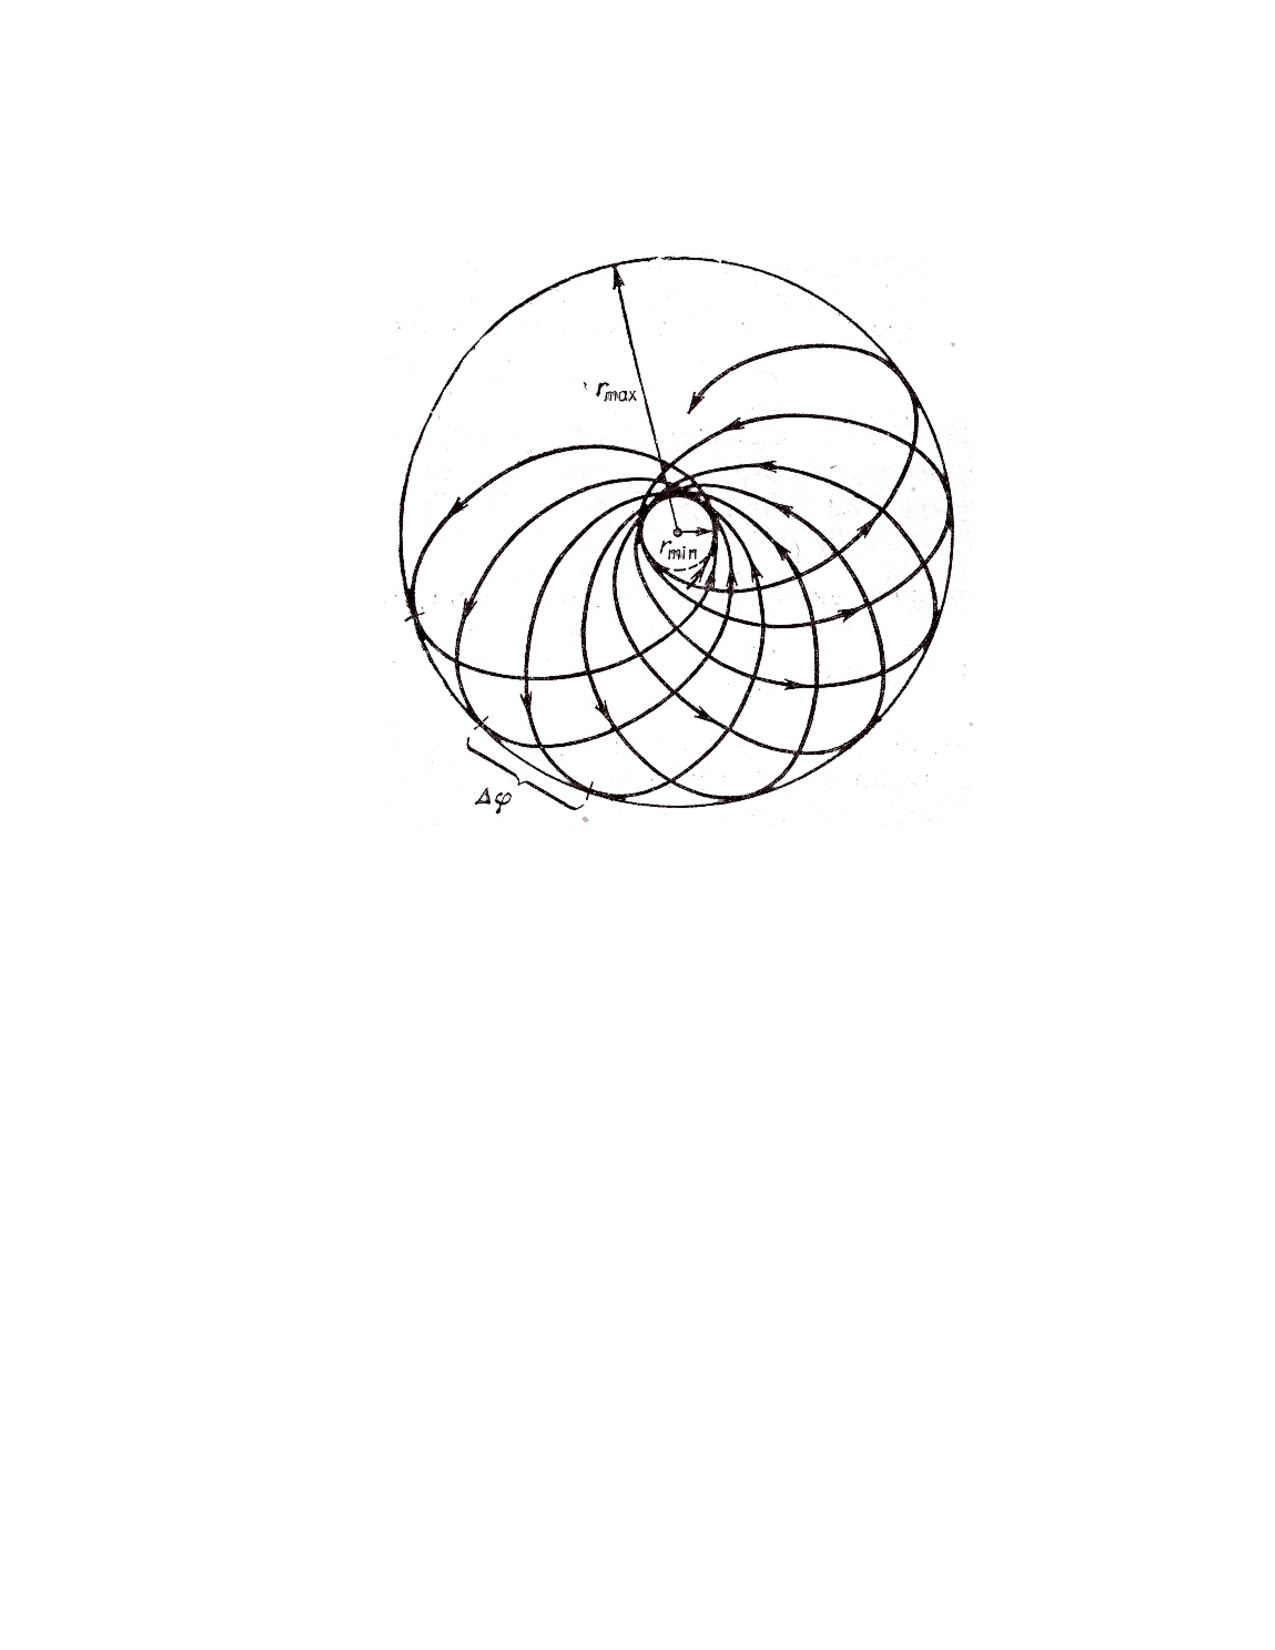
\includegraphics[width=0.5\linewidth]{images/annular-region.pdf}
    \caption{The trajectories are confined in an annular region \cite{book:ll}}
    \label{fig:annregio}
\end{figure}

\begin{exercise}
    Consider the integral \eqref{eq:deltaphi}, with $r_0 = r_m$ and $r = r_M$, one can use it to define the quantity
    \begin{equation}\label{eq:Dektaphi}
        \Delta \phi = 2\int_{r_m}^{r_M} \frac{\frac{M}{\rho^2}}{\sqrt{2m(E-U(\rho)) - \frac{M^2}{\rho^2}}}\;\d \rho.
    \end{equation}
    Prove that the motion is periodic if and only if
    \begin{equation}
        \Delta \phi = 2\pi \frac mn, \quad m,n\in\Z.
    \end{equation}
\end{exercise}

\subsection{Kepler's problem}

Let's go back to Example~\ref{ex:kepler2}, and replace $U$ with the Newtonian gravitational potential $k/\|\bx\|$ (see Examples~\ref{ex:Kepler0} and \ref{ex:kepler1}).
The effective potential \eqref{eq:effpotcp}, in this case is
\begin{align}
    U_{\mathrm{eff}} (r) = -\frac kr + \frac {M^2}{2 m r^2}, \quad &k = G \frac{m_1^2 m_2^2}{m_1+m_2} > 0,\\
    &m = \frac{m_1m_2}{m_1+m_2}, \quad M := M_z.
\end{align}
It's an exercise in calculus now, to see what this potential looks like.
The effective potential has a vertical asymptote at $r=0$, where it blows up to $+\infty$,
and the horizontal asymptote $y=0$ for $r\to+\infty$.
Finally, the potential presents a critical point, corresponding to a global minimum,
\begin{equation}
    U_{\mathrm{eff}}^* := U_{\mathrm{eff}}\left(\frac{M^2}{k m}\right) = - \frac{k^2m}{2M^2},
\end{equation}
after which the potential grows approaching $0$ as $r\to+\infty$.

\begin{figure}[th]
    \centering
    \begin{tikzpicture}
        \begin{axis}[
            xmin=-0.7,
            ymax=2,
            ymin=-2.5,
            xtick=\empty,
            ytick=\empty,
            axis lines=middle,
            xlabel=$r$,
            ylabel=$E$,
            y label style={at={(-0.03,0.995)}},
            axis on top,
        ]
        \addplot[blue,domain=0:15,samples=200,very thick]
            {-2/x + 1/(2*x^2)}
            node[pos=0.99] (Ulabel) {};
        \node [below, blue] at (Ulabel) {$U_{\mathrm{eff}}$};
        % Below
        \addplot [mark=none, gray!30!black, dotted, domain=-0.2:0.29289] {-1};
        \addplot [mark=none, red, domain=0.29289:1.70711, very thick] {-1} node[pos=2.5] (negelabel) {};
        \node [below, red] at (negelabel) {$U_{\mathrm{eff}}^* < E < 0$};
        \addplot [mark=none, gray!30!black, dotted, domain=1.70711:15] {-1};
        % Above
        \addplot [mark=none, gray!30!black, dotted, domain=-0.2:0.222474] {1};
        \addplot [mark=none, green!30!black, domain=0.222474:15, very thick] {1} node[pos=0.1] (poselabel) {};
        \node [below, green!30!black] at (poselabel) {$E > 0$};
        \end{axis}
    \end{tikzpicture}
    \label{fig:KeplerVeff}
    \caption{Kepler's problem $U_{\mathrm{eff}}$}
\end{figure}
In terms of phase portrait, this means that the motion is bounded if and only if
\begin{equation}
    - \frac{k^2 m}{2 M^2} < E < 0,
\end{equation}
and it is unbounded for $E \geq 0$.

The shape of the trajectory is then given by \eqref{eq:deltaphi}, which is explicitly solvable in this case:
\begin{equation}
    \phi = \arccos\left(\frac{\frac{M}{r}-\frac{km}{M}}{\sqrt{2mE + \frac{k^2m^2}{M^2}}}\right) + C,
\end{equation}
where the constant depends on the initial conditions.
Choosing $C=0$, we can rewrite the equation of the trajectory as
\begin{equation}\label{eq:KeplerConic}
    r = \frac{p}{1+e\,\cos\phi}, \qquad p:=\frac{M^2}{km}, \quad e:=\sqrt{1+\frac{2EM^2}{k^2 m}},
\end{equation}
which is the equation of a conic section with a focus at the origin, focal parameter $p$ and eccentricity $e$, in agreement with \emph{Kepler's first law}.
Choosing $C=0$, means that we have chosen the angle $\phi$ such that $\phi=0$ corresponds to the \emph{perihelion} of the trajectory, i.e. the closest point to the focus.
\medskip

We can now confirm the last claim in Example~\ref{ex:Kepler0}.
Indeed, with some knowledge about conic sections one can conclude that \eqref{eq:KeplerConic} is an ellipse for $E<0$, when $0<e<1$. The semiaxes of the ellipse are then given by
\begin{equation}
    a = \frac{p}{1-e^2}, \quad b = \frac{p}{\sqrt{1-e^2}}.
\end{equation}
Furthermore, when $E=0$, i.e. $e = 1$, we have a parabola and, finally, for $E>0$, i.e. $e >1$ an hyperbola.

We can also look at the time one body spends along parts of the orbit by looking at \eqref{eq:timedep}:
\begin{equation}
    t = \sqrt{\frac{m}{2}}
        \int \frac{\d r}{\sqrt{E - U_{\mathrm{eff}}(r)}}, \quad U_{\mathrm{eff}}(r) = -\frac kr + \frac {M^2}{2 m r^2}.
\end{equation}
In the case of elliptic trajectories $0<e<1$, despite its look, we can actually solve it with some smart chains of substitutions. Using
\begin{equation}
    M = \sqrt{kmp}, \quad E = -k \frac{1-e^2}{2p}, \quad\mbox{and}\quad p= a(1-e^2),
\end{equation}
and then the substitution
\begin{equation}\label{eq:rkp}
    r - a = - a e \cos \theta,    
\end{equation}
the integral becomes
\begin{align}
    t &= \sqrt{\frac {ma}k} \int \frac{r\d r}{\sqrt{-r^2 + 2ar -ap}} \\
      &= \sqrt{\frac {ma}k} \int \frac{r\d r}{\sqrt{a^2e^2 - (r-a)^2}} \\
      &= \sqrt{\frac{ma^3}{k}} \int (1- e \cos\theta) \d \theta \\
      &= \sqrt{\frac{ma^3}{k}} (\theta- e \sin\theta) + C. \label{eq:tkp}
\end{align}
By the arbitrariness of the choice of $t_0$, we can always choose $C=0$.

Together, \eqref{eq:rkp} and \eqref{eq:tkp}, provide a parametrization of the radial motion:
\begin{equation}
    \left\lbrace
    \begin{aligned}
        r &= a(1-e\cos\theta)\\
        t &= \sqrt{\frac{ma^3}k}(\theta - e\sin\theta)
    \end{aligned}
    \right..
\end{equation}
Given that $\theta\mapsto r(\theta)$ is $2\pi$ periodic, we can immediately obtain the period from $t(\theta)$:
\begin{equation}
    T = 2\pi \sqrt{\frac{ma^3}k}.
\end{equation}

To rewrite the orbits in cartesian coordinates, $x = r \cos\phi$, $y=r \sin\phi$, we can use the two representations for $r$
\begin{equation}
    \frac{p}{1+e\cos\phi} = r = a(1-e\cos\theta)
\end{equation}
to derive
\begin{equation}
    \cos\phi = -\frac{e - \cos\theta}{1-e \cos\theta},\quad
    \sin\phi = \frac{\sqrt{1-e^2}\;\sin\theta}{1-e\cos\theta},
\end{equation}
which, in turn, imply the parametrization in cartesian coordinates
\begin{equation}
    \left\lbrace
    \begin{aligned}
        x &= a(\cos\theta - e)\\
        y &= a\sqrt{1-e^2}\;\sin\theta\\
        t &= \sqrt{\frac{ma^3}k}(\theta - e\sin\theta)
    \end{aligned}
    \right..
\end{equation}

\begin{exercise}
    Obtain the following parametrization for the hyperbolic motion for $E>0$.
    \begin{equation}
        \left\lbrace
        \begin{aligned}
            x &= a(e- \cosh\xi)\\
            y &= a\sqrt{e^2-1}\;\sinh\xi\\
            t &= \sqrt{\frac{ma^3}k}(e\sinh\xi-\xi)
        \end{aligned}
        \right..
    \end{equation}
\end{exercise}

\begin{exercise}
    Obtain the following parametrization for the parabolic motion for $E=0$.
    \begin{equation}
        \left\lbrace
        \begin{aligned}
            x &= \frac p2 \left(1- \eta^2\right)\\
            y &= p\eta\\
            t &= \sqrt{\frac{mp^3}k}\frac\eta2\left(1+\frac{\eta^2}3\right)
        \end{aligned}
        \right..
    \end{equation}
\end{exercise}

It is possible to obtain an \emph{explicit} dependence on time with some extra effort by expanding the trigonometric terms in terms of Bessel functions. This is rather useful when studying certain type of orbit-orbit or spin-orbit resonances, but we will not investigate it further in this course. For additional information you can refer to \cite{book:arnoldcelestial, book:celletti}.

\begin{exercise}
    Let $0<e<1$ and $\tau = \theta - e\sin\theta$.
    Show that $\sin\theta$ and $\cos\theta$ can be expanded in Fourier series as
    \begin{align}
        \sin\theta &= \frac2e \sum_{n=1}^\infty \frac{J_n(ne)}{n} \sin(n\tau),\\
        \cos\theta &= -\frac e2 + 2 \sum_{n=1}^\infty \frac{J'_n(ne)}{n} \cos(n\tau),
    \end{align}
    where $J_n(x)$ are the Bessel functions of the first kind 
    \begin{equation}
        J_n(x) = \sum_{j=0}^\infty (-1)^j\frac{}{j!(j+n)!}\left(\frac z2\right)^{2j+n}, \quad n\in\N.
    \end{equation}

    \emph{Hint}: use the integral representation
    \begin{equation}
        J_n(z) = \frac1\pi \int_0^\pi \cos\left(z\sin\phi - n \phi\right)\d\phi,, \quad n\in\N.
    \end{equation}
\end{exercise}

In Example~\ref{ex:Kepler0}, we mentioned a third conserved quantity for the Kepler problem.
\begin{exercise}
    Show that the components of the Laplace-Runge-Lenz vector
    \begin{equation}
        \bm{L} := [\dot \bx, \bm{M}] - k \frac{\bx}{\|\bx\|}
    \end{equation}
    are first integrals for the Kepler problem.
\end{exercise}

\begin{exercise}
    Consider a small perturbation of the gravitational potential $U(r) = -\frac kr$ of the form
    \begin{equation}
        U(r) \mapsto U(r) + \epsilon \frac 1{r^2}.
    \end{equation}
    Use \eqref{eq:Dektaphi}, to compute a linear approximation in $\epsilon$ of the perturbation $\delta \phi$ of the perihelion of the elliptic orbit.
\end{exercise}

\section{D'Alembert principle and systems with constraints}\label{sec:LagrangeConstraints}

In most of the examples above, we have started by assuming that each particle is free to roam in $\R^3$.
However, in many instances this is not the case.
In this section we will briefly investigate how Lagrangian mechanics deals with these cases. For a different take on this problem, refer to \cite[Chapter 21]{book:arnold}.

If a free lagrangian for a point particle living on a surface $M$ in $\R^3$ were evolving according to the free euclidean Newton's law (without any potential), the particle would generally move in a straight line and not stay confined on the surface.
From the point of view of Newton, this means that there should be a virtual force that keeps the particle constrained to the surface. Of course, constraints could be more general than this.

Let's try again. Consider now a natural lagrangian \eqref{eq:mechlag}
\begin{equation}
    L(\bx, \dot\bx) = \sum_{j=1}^N \frac{m_j \dot \bx_j^2}{2} - U(\bx_1, \ldots, \bx_N)
\end{equation}
whose point particles are forced to satisfy a number of \emph{holonomic constraints}, i.e. relationships between the coordinates of the form
\begin{equation}\label{eq:holonomic}
    f_1(\bx_1, \ldots,\bx_N) = 0, \;\ldots,\; f_k(\bx_1, \ldots,\bx_N) = 0
\end{equation}
where $f_i : \R^{3N}\to\R$ smooth, $i=1,\ldots,k$.

\begin{remark}
    We call the constraints holonomic if the functions that define them do not depend on the velocities (they can depend on time, their treatment is analogous to what we will do in this section). More general constraints, also taking into account the velocities, are called \emph{non holonomic} and will not be treated in this course.
\end{remark}

Hamilton's principle is then applied to curves which satisfy the relations \eqref{eq:holonomic}, and whose fixed end points satisfy \eqref{eq:holonomic}.

\begin{tcolorbox}
    \emph{D'Alembert principle} states that the evolution of a mechanical system with constraints can be seen as the evolution of a closed system in the presence of additional forces called \emph{constraint forces}.
\end{tcolorbox}

To be more precise, assume that the $k$ equations \eqref{eq:holonomic} are \emph{independent}, i.e. that they define a smooth submanifold $Q\subset M$ of the configuration space $M=\R^{3N}$ with maximal dimension $\dim Q = 3N-k$.

As the tangent space $T_qQ \subset \R^{3N}$ is a linear subspace of the ambient tangent space $T_q \R^{3N}$, its orthogonal complement is a linear subspace of dimension $k$ spanned by the gradients of the functions $f_1, \ldots,f_k$.

\begin{theorem}
    The equations of motion of a mechanical system on $N$ particles with natural lagrangian \eqref{eq:mechlag} under the effect of $k$ independent holonomic constraints \eqref{eq:holonomic} have the form
    \begin{equation}\label{eq:generalnewtonconstraint}
        m_j \ddot \bx_j = - \frac{\partial U}{\partial \bx_j} + \bm{R}_j, \quad k=1, \ldots, N,
    \end{equation}
    where the \emph{constraint force} $\bm{R} = (\bm{R}_1, \ldots, \bm{R}_N)$ is orthogonal to the submanifold $Q$ defined by the constraints
    \begin{equation}\label{eq:orthogonalconstraint}
        \sum_{j=1}^N \left(\bm{R}_j, \delta\bx_j\right) = 0,
    \end{equation}
    for all vectors $\delta\bx = (\delta\bx_1,\ldots,\delta\bx_N)$ tangent to the submanifold $Q$.
\end{theorem}
\begin{proof}
    To deal with constraints in the lagrangian formulation, we introduce $k$ new variables $\lambda_1, \ldots, \lambda_k$, called \emph{Lagrange multipliers}, and define a new lagrangian
    \begin{equation}
        \tilde L(\bx, \dot\bx, t) = L(\bx, \dot\bx) + \sum_{j=1}^k \lambda_j(t)f_j(\bx).
    \end{equation}
    The evolution will be determined by the critical points for the corresponding action functional $\tilde S$.

    Since $\tilde L$ does not depend on $\dot\lambda$, the Euler-Lagrange equations for $\lambda$ are just
    \begin{equation}
        \frac{\partial \tilde L}{\partial \lambda_j} = f_j(\bx) = 0,\quad j=1,\ldots,k,
    \end{equation}
    which gives us back the constraints defining the submanifold $Q$.

    The other equations of motion, on the other hand, take the form
    \begin{equation}\label{eq:newtconstr}
        m_j \ddot \bx_j = -\frac{\partial U}{\partial\bx_j} + \sum_{i=1}^k \lambda_i(t) \frac{\partial f_i(\bx)}{\partial \bx_j},
        \quad j=1,\ldots,k.
    \end{equation}
    For all $i$, the vectors $\frac{\partial f_i(\bx)}{\partial \bx_j}$ are orthogonal to the submanifold $Q$, 
    \begin{equation}
        \sum_{i=1}^N \left(\frac{\partial f_i(\bx)}{\partial \bx_j}\right) = 0, \quad j=1,\ldots,k,
    \end{equation}
    and thus also their linear combinations $\bm{R}$ are, where 
    \begin{equation}
        \bm{R}_j := \sum_{i=1}^k \lambda_i(t) \frac{\partial f_i(\bx)}{\partial \bx_j},
        \quad j=1,\ldots,k.
    \end{equation}
\end{proof}

\begin{remark}
    The theorem above is often stated as follows: in a constrained system, the total work of the constraint forces on any virtual variations, i.e. vectors $\delta\bx$ tangent to the submanifold $Q$, is zero.
\end{remark}

Equations \eqref{eq:generalnewtonconstraint} and \eqref{eq:orthogonalconstraint} fully determine the evolution of the constrained system and the constraint forces.

Constrained motions have also a nice intrinsic description in terms of a mechanical system on $TQ$. Indeed, introducing local coordinates $q= (q_1, \ldots, q_n)\in Q$, where $n = 3N-k$, the substitution $\bx_j = \bx_j(q)$, $j=1,\ldots,N$ immediately implies the following theorem.

\begin{theorem}
    The evolution of of a mechanical system on $N$ particles with natural lagrangian \eqref{eq:mechlag} under the effect of $k$ independent holonomic constraints \eqref{eq:holonomic} can be described by mechanical system on $TQ$ with lagrangian
    \begin{equation}
        L_Q(q,\dot q) = \frac12 \sum_{i,j=1}^n g_{ij}(q)\dot q^i \dot q^j - U(\bx_1(q),\ldots,\bx_N(q)), \quad n = 3N-k,
    \end{equation}
    where
    \begin{equation}
        g_{ij}(q) = \sum_{l=1}^k m_l\left(\frac{\partial \bx_l}{\partial q^i},\frac{\partial \bx_l}{\partial q^j}\right)
    \end{equation}
    is the riemannian metric induced by the euclidean metric on $Q$ given by
    $ds^2 = \sum_{j=1}^N m_j(\d \bx_j, \d\bx_j)$.
\end{theorem}

This can be further generalized to mechanical systems which are constrained on the tangent bundle $TM$ of a manifold $M$ of dimension $n$.
In such case, let  $L=L(x,\dot x)$ be a non degenerate lagrangian on $TM$, and consider a smooth submanifold $Q\subset M$ of dimension $m$ with local coordinates $(q^1,\ldots,q^m)$.
Assume that $Q$ is \emph{regular} with respect to the lagrangian, i.e. such that the restriction of $\left(\frac{\partial^2 L}{\partial \dot x^i \partial\dot x^j}\right)_{i,j=1,\ldots,n}$ to $Q$ os still non degenerate:
\begin{equation}
    \det\left(\frac{\partial^2 L}{\partial \dot x^i \partial\dot x^j}\frac{\partial x^i}{\partial q^k}\frac{\partial x^j}{\partial q^l}\right)_{k,l=1,\ldots,m} \neq 0.
\end{equation}
As before we can define the constrained motion by minimizing the corresponding action restricted on the space of curves in $Q$ with the appropriate fixed endpoints in $Q$. Due to the immersion of $Q$ into $M$, which in coordinates reads $x^1 = x^1(q)$, $\ldots$, $x^n=x^n(q)$, and the corresponding immersion of tangent bundles, we can define the restriction of the lagrangian $L$ on the subbundle $TQ$:
\begin{equation}\label{eq:dalembertmanifold}
    L_q(q,\dot q) = L\left(x(q), \frac{\partial x}{\partial q}\dot q\right).
\end{equation}

\begin{exercise}
    Show that the equations of motion of the constrained motion on $Q$ are given by the Euler-Lagrange equations of the lagrangian \eqref{eq:dalembertmanifold}.
\end{exercise}

\begin{example}
    Every submanifold $Q\subset \R^n$ of the euclidean space is regular with respect to the free lagrangian
    \begin{equation}
        L = \frac12 \sum_{k=1}^n \dot x^2_k.
    \end{equation}
    The lagrangian $L_Q$ of the constrained motion has the form
    \begin{equation}
        L_Q = \frac12 \sum_{i,j=1}^m g_{ij}(q)\dot q^i\dot q^j, \qquad g_{ij}(q) = \sum_{k=1}^n \frac{\partial x_k}{\partial q^i}\frac{\partial x_k}{\partial q^j}.
    \end{equation}
    Here $g_{ij}$ is the riemannian metric induced on $Q$ by the euclidean metric $\d s^2 = \d x_1^2 + \cdots + \d x_n^2$.
    As we have already seen, the evolutions corresponding to $L_Q$ are the geodesics of such metric.
\end{example}

\begin{exercise}
    Consider the lagrangian $L=\frac12 g_{ij}(q)\dot q^i \dot q^j$ on the tangent bundle of a riemannian manifold $Q$ with a metric $\d s^2 = g_{ij}(q)\d q^i \d q^j$.
    Show that the solutions $q=q(t)$ of the Euler-Lagrange equations for $L$ satisfy $(\dot q, \dot q)= \mathrm{const}$.
\end{exercise}

\begin{exercise}[Clairaut's relation]
    Given a function $f(z): [a,b] \to \R_+$, consider the \emph{surface of revolution} in $\R^3$ implicitly defined by
    \begin{equation}
        \sqrt{x^2 + y^2} = f(z).
    \end{equation}
    Show that a curve is a geodesic on the surface if and only if it satisfies the following property: let $\phi$ be the angle that the geodesics makes with the parallel $z=\mathrm{const}$, then $f(z)\cos \phi = \mathrm{const}$.
\end{exercise}

\begin{example}[Double pendulum revisited]
    Let's see if we can re-derive the double pendulum lagrangian using D'Alembert principle.
    We have a system of two point masses with masses $m_1$ and $m_2$ connected by massless rigid rods: one of length $l_2$ connecting them to each other and one of length $l_1$ connecting the first to a pivot on the ceiling. We assume that frictions are absent and that the double pendulum is constrained to move in a single plane.

    A priori the position of the two masses is represented by a six dimensional vector
    $\bx = (x_1, y_1, z_1, x_2, y_2, z_2)\in\R^6$, with the additional constraints
    \begin{align}
        f_1(\bx) &= y_1 = 0,\\
        f_2(\bx) &= y_2 = 0,\\
        f_3(\bx) &= x_1^2 + z_1^2 - l_1^2 = 0,\\
        f_4(\bx) &= (x_2-x_1)^2 + (z_2-z_1)^2 - l_2^2 = 0,
    \end{align}
    representing the planar motion and the rods restrictions.

    The number of degrees of freedom is then $n = 6 -4 = 2$, and the two last equations should suggest that a good choice of coordinates would be the pair of angles describing the displacement of the mass from the respective joint vertical, as we did in Example \ref{ex:2pendulum}.
\end{example}

\begin{exercise}
    Use D'Alembert principle to compute the constraint force acting on the spherical pendulum under the effect of the gravitational potential.
    
    Assume, then, that the constraint force can act only radially outward. Imagine, for example that the point particle is a pebble set in motion on a frictionless and impenetrable ball of dry ice at rest.
    When and where will the particle leave the sphere?
\end{exercise}

%\section{Non inertial reference frames}
%\todo{Not treated in the course. Add later, examples of small oscillations on body falling on rotating Earth and Focault pendulum}

\chapter{Hamiltonian mechanics}

In this chapter we start our investigation of the hamiltonian formalism.
We have already seen glimpses of it throughout some of the exercises and examples in the previous chapter, but only scratched the surface.
We will see how this, seemingly harmless, change of perspective will reveal much more about the geometric structure underlying classical dynamics.

In the lagrangian formulation for a system with $n$ degrees of freedom and lagrangian function $L=L(q, \dot q)$, we have seen that the equations of motion are encoded by the Euler-Lagrange equations, which are $n$ second order differential equations in $q$, requiring $2n$ initial conditions, say $q(0)$ and $\dot q(0)$.

%The starting point for our investigation will be Theorems~\ref{thm:ham1} and~\ref{thm:conservationEnergy}, and Example~\ref{ex:natlagham}.
In the previous chapters, we saw that the $n$ generalized momenta
\begin{equation}
    p_i = \frac{\partial L}{\partial \dot q^i}, \quad i=1,\ldots,n,
\end{equation}
play a relevant role in the first integrals at the core of Noether theorem, and in particular in the conservation of energy.
If we then look at the Euler-Lagrange equations and revisit them in terms of the momenta, they acquire the nice form
\begin{equation}
    \dot p_i = \frac{\partial L}{\partial q^i}, \quad i=1,\ldots,n.
\end{equation}
Which seems to bring a nice symmetry between the coordinates and the momenta, and seems to allow us to reduce the problem to a first order system of equations.

Our current quest is then to find a function of $q$ and $p$ (and not of $\dot q$) which contains the same information as the lagrangian $L$, allowing us to determine the unique evolution of $q$ and $p$, but bringing the two variables to more equal footings.

Theorem~\ref{thm:ham1} and Theorem~\ref{thm:conservationEnergy} provided us with some useful hints.
Before entering into the gist of the matter, let's reason in two dimensions and mimick our derivation of Theorem~\ref{thm:ham1}

\section{The Legendre Transform in the euclidean plane}

In this section we'll be a bit sloppy, please bear with me. 
%
Let's start considering the total derivative of an arbitrary function $f(x,y)$,
\begin{equation}
    \d f = \frac{\partial f}{\partial x} \d x + \frac{\partial f}{\partial y} \d y,
\end{equation}
and defining a new function of three variables $x,y,u$:
\begin{equation}
    g(x,y,u) = ux - f(x,y).
\end{equation}
The total derivative of $g$ is then given by
\begin{equation}\label{eq:hamdgex}
    \d g = \d(ux) - \d f = u\d x + x \d u - \frac{\partial f}{\partial x} \d x - \frac{\partial f}{\partial y} \d y.
\end{equation}
Even though $u$ is a free variable, let's assume for the sake of the argument that we choose it to be a specific function of $x$  and $y$, say
\begin{equation}
    u(x,y) = \frac{\partial f}{\partial x}.
\end{equation}
Then \eqref{eq:hamdgex} simplifies into
\begin{equation}
    \d g = x \d u - \frac{\partial f}{\partial y} \d y,
\end{equation}
i.e. $g=g(y,u)$ could be considered a function of just $y$ and $u$.
Inverting $x = x(y,u)$, we could write down $g$ explicitly as
\begin{equation}
    g(y,u) = u x(y,u) - f(x(y, u), y).
\end{equation}

We have just described an operation which takes a function $f(x,y)$ to a different function $g(y,u)$ where $u = \frac{\partial f}{\partial x}$ \emph{without losing any information}: we can recover $f(x,y)$ from $g(y,u)$ by observing that
\begin{equation}
    \frac{\partial g}{\partial u} = x
    \quad\mbox{and}\quad
    \frac{\partial g}{\partial y} = - \frac{\partial f}{\partial y},
\end{equation}
which ensures that we can invert the transformation to get $f(x,y) = \frac{\partial g}{\partial u}u - g$.

We have just describe the Legendre transform.
If you look carefully you may recognize it in Theorem~\ref{thm:conservationEnergy}.

The geometrical meaning of the Legendre transform is best captured with a picture.
For a fixed $y$, draw the curves $f(x) = f(x,y)$ and $ux$. 
For each slope $u$, the value of $g(u) = g(u,y)$ measures the maximal distance between the two curves $f(x)$ and $ux$: finding the maximum of such distance means
computing
\begin{equation}
    \frac{\d}{\d x}(ux - f(x)) = 0 \quad\Rightarrow\quad u = \frac{\partial f}{\partial x}.
\end{equation}
Note that in the computation above we are assuming that a maximum exists:
this hints to the fact that the Legendre transformation can only be applied to \emph{convex functions}.

In the next section we will explicit this discussion rigorously and in greater generality.

\section{The Legendre Transform}

Let $M$ be a smooth manifold.
The evolution of the system with lagrangian $L=L(q,\dot q)$ is given by the Euler-Lagrange equations: a system of second order equations on the tangent bundle $TM$.
Such dynamics can be reinterpreted in a particularly symmetric way as a dynamical system on the cotangent bundle $T^*M$.
Poisson and Hamilton have formalized the transformation that we described in the previous section and that realizes such symmetry.

\begin{tcolorbox}
    We call \emph{Legendre transformation} the map from the tangent bundle $TM$ to the cotangent bundle $T^*M$ defined in local coordinates $(q^1, \ldots, q^n)\in M$ by 
    \begin{equation}\label{eq:legrendreTrafo}
        \cL: (q,\dot q) \mapsto (q,p),
    \end{equation}
    where $p = (p_1, \ldots, p_n) \in T^*_q M$ is the conjugate momentum to $q$ defined via $p_i := \frac{\partial L(q,\dot q)}{\partial \dot q^i}$, $i=1,\ldots,n$.
\end{tcolorbox}
It follows from Exercise~\ref{exe:coordinatesInd} that the definition above does not depend on the choice of local coordinates.

If it is not yet clear to you how the momenta are associated to the cotangent bundle, I promise you will not have to wait long. But if you are really impatient you could already have a look at Remark~\ref{rem:ptocot}.

\begin{theorem}
    The Legendre transform of a non--degenerate lagrangian is a local diffeomorphism.
\end{theorem}
\begin{proof}
    It is enough to show that Jacobian determinant of $\cL$ is non zero. From the definition, see \eqref{eq:legrendreTrafo}, we have the block matrix
    \begin{equation}
        D\cL = \begin{pmatrix}
            \frac{\partial q^i}{\partial q^j} & \frac{\partial q^i}{\partial \dot q^j} \\
            \frac{\partial p_i}{\partial q^j} & \frac{\partial p_i}{\partial \dot q^j}
        \end{pmatrix}
        = \begin{pmatrix}
            \delta^i_j & 0 \\
            \frac{\partial^2 L}{\partial \dot q^i \partial q^j} & \frac{\partial^2 L}{\partial \dot q^i  \partial \dot q^j},
        \end{pmatrix},
    \end{equation}
    From which we get
    \begin{equation}
        \det D\cL = (-1)^n \det\left(\frac{\partial^2 L}{\partial \dot q^i  \partial \dot q^j}\right) \neq 0.
    \end{equation}
\end{proof}

It follows that for a non--degenerate lagrangian we can locally invert the equations
\begin{equation}
    p_i = \frac{\partial L(q,\dot q)}{\partial \dot q^i}, \; i=1,\ldots,n,
\end{equation}
and write
\begin{equation}
    \dot q^i = \dot q^i(q,p).
\end{equation}
In this way, every non--degenerate function on $TM$ defines a function on $T^* M$.

\begin{tcolorbox}
    We call \emph{hamiltonian} of a mechanical system with lagrangian $L$, the Legendre transform $H(q,p)$ of its energy $E(q,\dot q)$ from \eqref{eq:energy1}.
    In local coordinates the hamiltonian of the system is given by
    \begin{equation}\label{eq:defH}
        H(q,p) := p_i\dot q^i - L(q, \dot q), \quad \dot q^i = \dot q^i(q,p).
    \end{equation}  
\end{tcolorbox}

\begin{remark}
This is what is meant when you read that the hamiltonian is the lift of the total energy $E(q, \dot q)$ of the system to a function $H(q,p)$ on the cotangent bundle $T^*M$.
\end{remark}

The crucial point of this whole construction lies in the new shape taken by the Euler-Lagrange equations once we revisit them on the cotangent bundle.

\begin{theorem}[Hamilton's equations]\label{thm:Hameqns}
    Euler-Lagrange equations for a lagrangian $L(q,\dot q)$ are equivalent to \emph{Hamilton's equations}
    \begin{equation}\label{eq:Hamsys}
        \left\lbrace
        \begin{aligned}
            \dot q^i &= \frac{\partial H}{\partial \dot p_i}\\
            \dot p_i &= -\frac{\partial H}{\partial \dot q^i}
        \end{aligned}
        \right. \qquad i=1,\ldots,n,
    \end{equation}
    for the corresponding hamiltonian $H(q,p)$.
\end{theorem}
\begin{proof}
    The differential of the hamiltonian,
    \begin{equation}\label{eq:dHlc}
        \d H(q,p) = \frac{\partial H}{\partial q^i}\d q^i + \frac{\partial H}{\partial p_i}\d p_i,
    \end{equation}
    can be explicitly computed using its definition:
    \begin{align}
        \d H(q,p) &= \d \left( p_i\dot q^i(q,p) - L(q, \dot q(q,p)) \right) \\
        &= \dot q^i \d p_i + p_i \d \dot q^i(q,p) - \frac{\partial L}{\partial q^i} \d q^i - \frac{\partial L}{\partial \dot q^i} \d \dot q^i \\
        &= \dot q^i \d p_i - \dot p_i \d q^i, \label{eq:dHlc2}
    \end{align}
    where we used the Euler-Lagrange equations to get
    \begin{equation}
        p_i = \frac{\partial L}{\partial \dot q^i}
        \qquad\mbox{and}\qquad
        \dot p_i = \frac{\d }{\d t}\frac{\partial L}{\partial \dot q^i} = \frac{\partial L}{\partial q^i}.
    \end{equation}
    The theorem follows comparing coefficients in \eqref{eq:dHlc} and \eqref{eq:dHlc2}.
\end{proof}
We call \emph{hamiltonian system} a system of differential equations of the form \eqref{eq:Hamsys} and, as one can expect, we say that $H$ is its corresponding hamiltonian function. Equations of the form \eqref{eq:Hamsys} are usually called \emph{canonical equations}.

\begin{example}[A particle in a potential]\label{ex:hamPot}
    Let's start with a simple prototypical example: a particle in $\R^3$ moving under the influence of a potential $U(\bx)$.
    We are, by now, very accustomed to the corresponding natural lagrangian
    \begin{equation}
        L(\bx,\dot \bx) = \frac{\dot \bx^2}{2m} - U(\bx).
    \end{equation}
    In this case
    \begin{equation}
        \bp = \frac{\partial L}{\partial \dot \bx} = m \dot\bx
    \end{equation}
    coincides with what we usually call (kinetic) momentum in physics.

    The hamiltonian is then given by
    \begin{equation}
        H(\bp,\bx) = (\bp, \dot\bx) - L = \frac {m\bp^2}2 + U(\bx),
    \end{equation}
    which should remind you of Theorem~\ref{thm:ham1}.
    Hamilton's equation are then simply
    \begin{equation}
        \left\lbrace
        \begin{aligned}
            \dot \bx &= \frac{\partial H}{\partial \bp} = \frac1m \bp\\
            \dot {\bp} &= - \frac{\partial H}{\partial \bx} = -\frac{\partial U}{\partial \bx}
        \end{aligned}
        \right.,
    \end{equation}
    which should also be familiar: the first is just the definition of momentum while the second is Newton's second law for the system.
\end{example}

\begin{example}[The hamiltonian for a natural lagrangian on a riemannian manifolds]\label{ex:nlrm}
Let $L$ be a free lagrangian
\begin{equation}
    L(q, \dot q) = \frac12 g_{ij}(q) \dot q^i \dot q^j
\end{equation}
on the tangent bundle $TM$ of a riemannian manifold $(M,g)$.
Recall that
\begin{equation}
    \d s^2 = g_{ij}(q)\d q^i \d q^j.
\end{equation}
Denote $(g^{ij}(q))$ the inverse of the metric matrix $(g_{ij}(q))$, i.e. the matrix such that $g_{ik}(q)g_{kj}(q) = \delta^i_j$ for all $i,j=1,\ldots,n$.

The Legendre transform of $L$ is, then, the hamiltonian
\begin{equation}
    H = \frac12 g^{ij}(q) p_i p_j,\quad\mbox{with}\quad
    p_i := g_{ij}(q)\dot q^j, \; i = 1,\ldots, n,
\end{equation}
while the inverse transform gives $L$ in terms of
\begin{equation}
    \dot q^i = g^{ij}(q) p_j, \quad i = 1,\ldots, n.
\end{equation}

As we saw when we defined the Legendre transform and in Exercise~\ref{exe:coordinatesInd}, the behavior of the metric tensor under coordinate transformations implies that $H$ is invariant under a change of variable.
Moreover, we saw in Exercise~\ref{exe:geodesic1} that geodesics on $M$ are the solutions of the Euler-Lagrange equation for the free lagrangian $L$.
But then, Theorem~\ref{thm:Hameqns} implies that geodesics should appear also from the flow of Hamilton's equation
\begin{equation}\label{eq:geoflowham}
    \left\lbrace
    \begin{aligned}
        \dot q^i &= \frac{\partial H}{\partial p_i} = g^{ij}(q) p_j\\
        \dot p_i &= -\frac{\partial H}{\partial q^i} = -\frac12 \frac{\partial g^{jk}}{\partial q^i} p_j p_k
    \end{aligned}
    \right.
    \qquad i=1,\ldots,n.
\end{equation} 
Indeed, we can describe the geodesics in terms of the flow determined by \eqref{eq:geoflowham}, also called the \emph{cogeodesic flow}:
the geodesics are the projections of the integral curves of the (co)geodesic flow onto the manifold $M$.

\begin{exercise}
    Show that a simple substitution allows to recover Euler-Lagrange equations of Exercise~\ref{exe:geodesic1}, which gives the geodesic flow on the tangent bundle $TM$.
\end{exercise}

As we know that the hamiltonian is the total energy of the system and that the total energy is conserved, this immediately implies that $g_{ij}(q) \dot q^i \dot q^j = (\dot q, \dot q) = \mathrm{const}$. Which is one of our previous exercises.
\end{example}

\begin{remark}\label{rem:ptocot}
The previous example provides a good opportunity to discuss the nature of the momentum.
Let $(M, g)$ be a riemannian manifold.
The riemannian metric, or riemannian metric tensor, is a bilinear form $(\cdot, \cdot)$ on the tangent spaces of $M$.
In local coordinates $q\in M$, we can associate to the metric a matrix $g_{ij}(q)$.
With an abuse of notation, we say that $g_{ij}(q)$ is a $(0,2)$-tensor.

Every $(0,2)$-tensor $g_{ij}(q)$ canonically defines a map
\begin{equation}
    \hat g: TM \to T^*M, \qquad T_q M \ni v \mapsto \hat g_q(v) := p := (v, \cdot) \in T^*_q M.
\end{equation}
Such tensor is called \emph{non--degenerate} if the map $T_qM \to T_q^* M$ is an isomorphism for all $q\in M$.
Such isomorphism allows one to identify tangent and cotangent spaces and, in particular, to define a dual bilinear form $(\cdot, \cdot)^*$ on $T^*M$ using the original form on $TM$:
\begin{equation}
    (w_1, w_2)^* = (\hat g_q^{-1} w_1, \hat g_q^{-1} w_2), \quad w_1,w_2 \in T^*_q M.
\end{equation}
The matrix of this dual form coincides with the inverse of the metric matrix:
\begin{equation}
    (\d q^i, \d q^j)^* = g^{ij}(q).
\end{equation}
Which, in more algebraic terms and with the same abuse of notation, means that the inverse matrix $(g^{ij}(q))$ is a $(2,0)$-tensor.

The isomorphisms between the tangent and cotangent spaces defined above are what is commonly known as \emph{musical isomorphism}: the \emph{flat} and \emph{sharp} maps respectively correspond to the mapping $\beta:TM\to T^*M$ and $\sharp:T^*M\to TM$ such that $v^\beta(w) = (v,w)$ and $(p^\sharp, v) = p(v)$. See also \cite[Chapter 11]{book:lee}.
\end{remark}

\begin{example}
    We saw in Example~\ref{ex:hamPot} that the hamiltonian of a free particle of mass $m$ is, in cartesian coordinates,
    \begin{equation}
        H = \frac{1}{2m}(p_x^2 + p_y^2 + p_z^2).
    \end{equation}

    The preliminary computations that we did in Section~\ref{sec:lagrangianonmanifold} and Examples~\ref{ex:nlrm} immediately tell us how to compute the corresponding hamiltonian in cylindrical and spherical coordinates.
    Namely, we can invert the metric matrix to get
    \begin{align}
        \mbox{cylindrical coordinates } (r,\phi,z) \quad&\Rightarrow\quad H = \frac 1{2m} \left(p_r^2 + \frac{p_\phi^2}{r^2} + p_z^2\right), \\
        \mbox{spherical coordinates } (r,\phi,\theta) \quad&\Rightarrow\quad H = \frac 1{2m} \left(p_r^2 + \frac{p_\phi^2}{r^2\sin^2\theta} + \frac{p_\theta^2}{r^2} \right).
    \end{align}

    More generally, a natural lagrangian
    \begin{equation}
        L(q,\dot q) = \frac 12 g_{ij}(q) \dot q^i \dot q^j - U(q)
    \end{equation}
    on the tangent bundle of a riemannian manifold $(M,g)$ is transformed into a hamiltonian of the form
    \begin{equation}
        H(q,p) = \frac 12 g^{ij}(q) p_i p_j + U(q).
    \end{equation}

    Of course, one can also obtain the formulas above directly using Example~\ref{ex:nlrm} and Exercise~\ref{exe:coordinatesInd}.
\end{example}

\begin{exercise}[Inverse Legendre transform]
    Show that the hamiltonian $H$ defined by \eqref{eq:defH} satisfies the non--degeneracy condition
    \begin{equation}
        \det\left(\frac{\partial^2 H}{\partial p_i\partial p_j}\right) \neq 0.
    \end{equation}
    Moreover, the inverse Legendre transform can be written in local coordinates as
    \begin{equation}\label{eq:inverseLegendre}
        L(q, \dot q) = p_i \dot q^i - H,\qquad
        \dot q^i = \frac{\partial H (q,p)}{\partial p_i}, \; i=1,\ldots,n.
    \end{equation}
\end{exercise}

\begin{exercise}\label{exe:timedep}
    Show that the Legendre transform of a non--degenerate time-dependent lagrangian $L(q,\dot q, t)$ is well defined, the corresponding hamiltonian is
    \begin{equation}
        H(q,p,t) := p_i \dot q^i - L(q, \dot q, t),
    \end{equation}
    and Hamilton's equations have the same form plus an additional equation
    \begin{equation}
        \frac{\partial H}{\partial t} = - \frac{\partial L}{\partial t}.
    \end{equation}
    Note that such additional equation immediately implies that the total energy is not conserved for lagrangians or hamiltonians which are explicitly dependent on time.
\end{exercise}

\begin{example}[A particle in an electromagnetic field]\label{exe:magneticH}
We saw the Lagrangian for charged particles in an electromagnetic field in Example~\ref{exa:magnetic} and in Exercise~\ref{exe:magnetic}.
In the simpler case of a single particle, the lagrangian takes the form 
\begin{equation}
    L(\bx,\dot \bx) = \frac{m \dot{\bx}^2}{2} - U(\bx) + \frac ec (\bm A(\bx), \dot \bx).
\end{equation}
The conjugate momentum to the position is then given by
\begin{equation}\label{eq:magMom}
    \bp = \frac{\partial L}{\partial \dot \bx} = m \dot\bx + \frac{e}{c}\bm A(\bx)
\end{equation}
which now differs from what we usually call momentum by the additional term containing the magnetic vector potential $\bm A$.

Inverting \eqref{eq:magMom}, we get
\begin{equation}
    \dot\bx = \frac1m \left( \bp - \frac{e}{c}\bm A(\bx) \right),
\end{equation}
so the hamiltonian is
\begin{align}
    H(\bx, \bp) &= (\bp, \dot\bx) - L \\
    &= \frac1m\ \left( \bp, \bp - \frac{e}{c}\bm A(\bx)\right) -
        \frac1{2m}\left(\bp - \frac{e}{c}\bm A(\bx)\right)^2 \\
        &\quad + U(\bx)
        - \frac e{mc} \left(\bm A(\bx), \bp - \frac{e}{c}\bm A(\bx)\right)
        \\
    &= \frac1{2m}\left(\bp - \frac{e}{c}\bm A(\bx)\right)^2 + U(\bx).
\end{align}
The corresponding Hamilton's equation read
\begin{equation}
    \left\lbrace
    \begin{aligned}
        \dot \bx_i &= \frac{\partial H}{\partial \bp_i} = \frac1m \left(\bp_i - \frac{e}{c}(\bm A(\bx))^i\right)\\
        \dot \bp_i &= -\frac{\partial H}{\partial \bx_i} = -\frac{\partial U(\bx)}{\partial \bx_i} + \frac{e}{mc} \left(\bp_j - \frac{e}{c}(\bm A(\bx))^j\right)\frac{\partial (\bm A(\bx))^j}{\partial \bx_i}
    \end{aligned}
    \right.
\end{equation}
where $i=1,2,3$.

With some additional work, one can show that these are equivalent to Newton's second law with the additional Lorenz force as in Exercise~\ref{exe:magnetic}.
\end{example}

\begin{example}[A particle in a constant magnetic field]
An important special case of Example~\ref{exe:magneticH} is the case of a uniform magnetic field pointing in the $z$-direction: $\bm B = (0,0,B)$.
One convenient choice of vector potential for $\bm B$ is
\begin{equation}
    \bm A (x,y,z) = (-B y, 0, 0).
\end{equation}

Consider a particle moving in the $(x, y)$-plane.
Then, $p_z = 0$ and the Hamiltonian for the system is
\begin{equation}
    H = \frac1{2m}\left(p_x + \frac ec By\right)^2 + \frac1{2m}p_y^2.
\end{equation}
Hamilton's equations are four first order differential equations:
\begin{equation}\label{eq:magHeq}
    \left\lbrace
    \begin{aligned}
        \dot p_x &= 0 \\
        \dot x &= \frac1m\left(p_x + \frac ec By\right)\\
        \dot p_y &= -\frac{eB}{cm} \left(p_x + \frac ec By\right)\\
        \dot y &= \frac {p_y} m\\
    \end{aligned}
    \right.
\end{equation}

With some algebraic manipulations it is possible to show that there are the following additional conserved quantities (try to show it as an \textbf{exercise}):
\begin{equation}
    p_y + \frac ec Bx = \alpha = \mathrm{const} \quad\mbox{and}\quad
    p_x = m\dot x - \frac ec By = \beta = \mathrm{const}.
\end{equation}
With these at hand, Hamilton's equation become very easy to solve: we have
\begin{equation}
    x(t) = \frac {c \alpha}{e B} + R \sin(\omega t + \phi)
    \quad\mbox{and}\quad
    y(t) = -\frac {c \beta}{e B} + R \cos(\omega t + \phi),
\end{equation}
where $\alpha, \beta, R, \phi$ are integration constants and
\begin{equation}
    \omega = \frac{e B}{m c}.
\end{equation}
We see that the particle move in circles (\emph{gyration}) in the $(x,y)$-plane with frequency $\omega$, better known as \emph{Larmor or cyclotron frequency}.

Finally, observe from the first equation in \eqref{eq:magHeq} that $x$ being a cyclic coordinate is reflected also in the hamiltonian formalism as the conservation of momentum.
\end{example}

\begin{example}[The relativistic hamiltonian]
    If $c>0$ denotes the speed of light, the hamiltonian $H:\R^3\times\R^3\to\R$ of a free relativistic particle of mass $m>0$ is
    \begin{equation}
        H(q,p) = c \sqrt{p^2 + m^2 c^2}.
    \end{equation}
    For $p < c$ we can expand it in Taylor series as
    \begin{equation}
       H(q,p) = mc^2 + \frac{p^2}{2m} + O(p^4).
    \end{equation}
    If we interpret $H$ as the total energy, you can recognize a famous formula in the first term (also called \emph{rest energy}), while the second term is the non-relativistic kinetic energy.

    In this case, independently of the chosen momentum, the velocity
    \begin{equation}
        \dot q = \frac{\partial H}{\partial p} = c \frac{p}{\sqrt{p^2 + m^2 c^2}}
    \end{equation}
    is always strictly smaller, in absolute value, than the speed of light $c$.
    The corresponding Lagrangian $L$,
    \begin{equation}
        L(q,\dot q) = (\dot q, p(\dot q)) - H(q, p(\dot q)) = -mc^2 \sqrt{1-\frac{\dot q^2}{c^2}}
    \end{equation}
    is not defined on the whole $\R^3\times\R^3$! This is because the hamiltonian is degenerate: as you can check computing the determinant of the matrix $\frac{\partial^2 H}{\partial p^2}$.
\end{example}

\section{Poisson brackets and first integrals of motion}\label{sec:poisson}

One of the many advantages of the hamiltonian approach comes from an elegant algebraic description.
This will play a central role in the study of conserved quantities, and provides a remarkable duality with the mathematical description of quantum mechanics.

From now on, we will denote by $q = (q^1, \ldots, q^n)$ the local coordinates on $M$, and $(q^1, \ldots, q^n, p_1, \ldots, p_n)\in T^*M$ the coordinates induced by $q$ on $T^*M$. We will, thus, write functions on the cotangent space as $f=f(q,p)$.

\begin{tcolorbox}
    Let $f=f(q,p)$ and $g=g(q,p)$ be two functions on the phase space $T^*M$.
    Then the \emph{Poisson bracket} is defined to be
    \begin{equation}\label{def:Poisson}
        \big\{f,g\big\} = \frac{\partial f}{\partial q^i}\frac{\partial g}{\partial p_i} - \frac{\partial f}{\partial p_i}\frac{\partial g}{\partial q^i},
    \end{equation}
    where as usual we are summing repeated indices.
\end{tcolorbox}

\begin{exercise}
    Show that the definition of Poisson brackets on $T^*M$ does not depend on the choice of the local coordinates on $M$.
\end{exercise}

Since \ref{def:Poisson} is a kind of weird definition, let’s look at some of its properties.

\begin{theorem}\label{thm:PoissonLieAlgebra}
    Poisson bracket defines a structure of Lie algebra on the space $\cC^\infty(T^*M)$ of smooth functions on the phase space.

    More explicitly, the operation $\cC^\infty(T^*M)\times \cC^\infty(T^*M) \to \cC^\infty(T^*M)$ defined by $(f,g) \mapsto \big\{f,g\big\}$ satisfies the following properties for any $f,g,h \in \cC^\infty(T^*M)$:
    \begin{enumerate}
        \item it is antisymmetric, $\big\{g,f\big\} = - \big\{f,g\big\}$;
        \item it is bilinear, $\big\{\alpha f + \beta g, h\big\} = \alpha\big\{f,h\big\} + \beta\big\{g,h\big\}$ and $\big\{f, \alpha g + \beta h\big\} = \alpha\big\{f,g\big\} + \beta\big\{f,h\big\}$ for any $\alpha, \beta \in\R$;
        \item it fulfils \emph{Jacobi identity}: 
        \begin{equation}\label{eq:JacobiId}
            \big\{\big\{f,g\big\},h\big\} + \big\{\big\{h,f\big\},g\big\} + \big\{\big\{g,h\big\},f\big\} = 0.
        \end{equation}
    \end{enumerate}
    Finally, the Poisson bracket satisfies \emph{Leibnitz rule} with respect to function products:
    \begin{equation}\label{eq:LeibnitzId}
        \big\{fg, h\big\} = g\big\{f, h\big\} + f \big\{g, h\big\}, \qquad f,g,h \in \cC^\infty(T^*M).
    \end{equation}
\end{theorem}

The only property requiring a proof is the Jacobi identity.
Here I quote \cite{lectures:tong}:
\begin{quote}
    To prove this you need a large piece of paper and a hot cup of coffee. Expand out all 24 terms and watch them cancel one by one.
\end{quote}

What Theorem~\ref{thm:PoissonLieAlgebra} is telling us, is that Poisson's bracket define the same algebraic structure as matrix commutators and differential operators.
There is a deep relationship between what we are seeing here and Heisenberg's and Schr\"odinger's picture of quantum mechanics.
This relationship is emphasized even more if we compute the Poisson bracket of the coordinate functions:
\begin{equation}\label{eq:coordcommutators}
    \big\{q^i,p_j\big\} = \delta^i_j, \qquad \big\{q^i,q^j\big\} = \big\{p_i,p_j\big\} = 0, \qquad i,j = 1,\ldots,n.
\end{equation}

One crucial property of the Poisson bracket is enunciated by the following theorem.

\begin{theorem}\label{thm:poissondtdF}
    Let $H=H(q,p)$ be the hamiltonian of an hamiltonian system \eqref{eq:Hamsys} and $F=F(q,p)\in\cC^\infty(T^*M)$.
    Then,
    \begin{equation}
        \frac{\d}{\d t} F = \frac{\partial F}{\partial q^i} \dot q^i + \frac{\partial F}{\partial p_i} \dot p_i = \big\{F,H\big\}.
    \end{equation}
\end{theorem}

We say that two functions $H$ and $F$ on $T^* M$ \emph{commute}, or \emph{are in involution}, if
\begin{equation}
    \big\{H,F\big\} = 0.
\end{equation}
Then Theorem~\ref{thm:poissondtdF} implies the following.
\begin{corollary}
    Given an hamiltonian system \eqref{eq:Hamsys} with hamiltonian $H$ and a smooth function $F$ on its phase space, then $F$ is a first integral if and only if $H$ and $F$ are in involution.
\end{corollary}

This corollary implies some further interesting corollaries.
\begin{corollary}
    The first integrals of a hamiltonian system form a subalgebra of the Lie algebra $\cC^\infty(T^*M)$.
    Otherwise said, given two first integrals $F$ and $G$ of a hamiltonian system, then also the function $\big\{F,G\big\}$ is a first integral of $H$.
\end{corollary}
\begin{proof}
    By the previous corollary $\big\{F,H\big\} = \big\{G,H\big\} = 0$.
    Jacobi identity then implies that $\big\{\big\{F,G\big\},H\big\} = 0$, i.e. $\big\{F,G\big\}$ is a first integral of $H$.
\end{proof}

\begin{corollary}
    The hamiltonian function $H$ is a first integral of the hamiltonian system \eqref{eq:Hamsys}.
\end{corollary}
Which is the hamiltonian version of the conservation of energy, see Theorem~\ref{thm:conservationEnergy}.
In fact, we can reformulate this corollary as follows.
\begin{corollary}
    The integral curves $p = p(t)$ and $q=q(t)$ of the hamiltonian system \eqref{eq:Hamsys} belong to the levelset of the hamiltonian function, i.e.
    \begin{equation}
        H(q(t), p(t)) = \mathrm{const}.
    \end{equation}
\end{corollary}

\subsection{The symplectic matrix}\label{sec:symplmat}
    Denote the $2n$ coordinates on $T^*M$ as
    \begin{equation}
        x=(x^1, \ldots, x^{2n}) := (q^1, \ldots, q^n, p_1, \ldots, p_n).
    \end{equation}
    With this notation, the hamiltonian system \eqref{eq:Hamsys} takes the form
    \begin{equation}
        \dot x^k = \big\{x^k, H\big\}, \qquad k=1,\ldots,2n.
    \end{equation}
    
    We can write the Poisson bracket of the coordinate functions \eqref{eq:coordcommutators} as
    \begin{equation}
        \big\{x^k, x^l\big\} = J^{kl}, \qquad k,l = 1,\ldots,2n,
    \end{equation}
    where $J^{kl}$ are the matrix elements of the following antisymmetric matrix, called the \emph{symplectic matrix},
    \begin{equation}\label{eq:symmat}
        J = \left(J^{kl}\right)_{1\leq k,l\leq2n} = \begin{pmatrix}0 & \Id_n \\ -\Id_n & 0\end{pmatrix}.
    \end{equation}
    Then formula \eqref{def:Poisson} for the Poisson bracket of two arbitrary functions takes the following form
    \begin{equation}\label{eq:coordPB}
        \big\{f,g\big\} = J^{kl} \frac{\partial f}{\partial x^k}\frac{\partial g}{\partial x^l},
    \end{equation}
    and the hamiltonian system \eqref{eq:Hamsys} can be rewritten as
    \begin{equation}
        \dot x^k = J^{kl} \frac{\partial g}{\partial x^l}, \qquad k=1,\ldots,2n,
    \end{equation}
    or, more compactly,
    \begin{equation}\label{eq:hamsysJ}
        \dot x = J \frac{\partial H}{\partial x}.
    \end{equation}

\subsection{A brief detour on time-dependent hamiltonians}\label{sec:timedepH}

Let $L=L(q,\dot q,t): TM\times\R\to\R$, $q=(q^1,\ldots,q^n)\in M$, be the time-dependent lagrangian of some mechanical system as in Exercise~\ref{exe:timedep}.

Also in this case we can arrive to canonical equations of the form \eqref{eq:Hamsys}, however these will be on the extended space $T^*M\times\R^2$. The local coordinates $(q^1,\ldots,q^n, p_1, \ldots,p_n, q^{n+1}, p_{n+1})$ on $T^*M\times\R^2$ are such that $q^i, p_i$ remain the same for $i\leq n$,
\begin{equation}
    q^{n+1} = t, \quad\mbox{and}\quad
    p_{n+1} = -E,
\end{equation}
where $E$ is a new independent variable.
The hamiltonian then becomes
\begin{align}
    \hat H &= H(q^1, \ldots, q^n, p_1, \ldots, p_n) + p_{n+1}\dot q^{n+1} \\
    &= H(q^1, \ldots, q^n, p_1, \ldots, p_n) - E
\end{align}
where $H$ is given by the usual formula
\begin{equation}
    H = \sum_{i=1}^n p_i \dot q^i - L(q, \dot q, t), \quad \dot q^i = \dot q^i(q,p,t).
\end{equation}

The corresponding hamiltonian system is
\begin{align}
    & \dot q^i = \frac{\partial \hat H}{\partial p_i}, \quad 
      \dot p_i = -\frac{\partial \hat H}{\partial q^i}, \quad
      i=1,\ldots,n\\
    & \dot t = \frac{\partial \hat H}{\partial (-E)} = 1, \quad {(-\dot E)} = -\frac{\partial \hat H}{\partial t}.
\end{align}
The first $2n$ equations above are equivalent to the Euler-Lagrange equations for $L$ and the equation for $q^{n+1} = t$ tells us that $t$ is the same as in the original lagrangian and the final equation is simply the variation of the energy
\begin{equation}
    \dot E = \frac{\partial H}{\partial t}.
\end{equation}
which is the additional equation appearing 
If we restrict ourselves to the levelset $H - E = \hat H = 0$, then $E$ needs to satisfy the additional equation for the energy
\begin{equation}
    E = H = \sum_{i=1}^n p_i \dot q^i - L(q, \dot q, t),
\end{equation}
which completes the recovering of the original dynamics.

\section{Variational principles of hamiltonian mechanics}

Given a hamiltonian system $h$, can we describe its solutions of $q=q(t)$, $p=p(t)$ in terms of a variational principle as we do in Lagrangian mechanics?

A natural way to approach this question is to go back to Hamilton's variational principle, see Section~\ref{sec:varpri}, and use \eqref{eq:inverseLegendre} to invert Legendre transformation.
In fact, this is not in vane and one ends up showing the following theorem.

\begin{theorem}\label{thm:variationalHamilton}
    The solutions of a hamiltonian system \eqref{eq:Hamsys} with hamiltonian $H=H(q,p)$ are the critical points of the functional
    \begin{equation}\label{eq:variationalHamilton}
        S = \int_{t_1}^{t_2} \left(p_i\dot q^i - H(q,p)\right) \d t,
        \quad q(t_1) = q_1, \quad q(t_2) = q_2.
    \end{equation}
\end{theorem}
Note that, in this case, even though $p$ and $q$ play a rather symmetric role, we only fix the values of $q$ at the endpoints $t=t_1$ and $t=t_2$, while $p$ can be arbitrary.

\begin{proof}
    Computing the variation of the action $\delta S = S[q+\delta q, p + \delta p]$, one finds
    \begin{align}
        \delta S
        &= \int_{t_1}^{t_2} \left( \dot q^i \delta p_i + p_i \delta \dot q^i - \frac{\partial H}{\partial q^i}\delta q^i - \frac{\partial H}{\partial p_i}\delta p_i \right) \d t \\
        &= p_i \delta q^i\Big|_{t_1}^{t_2} + \int_{t_1}^{t_2} \left( \dot q^i \delta p_i + \dot p_i \delta q^i - \frac{\partial H}{\partial q^i}\delta q^i - \frac{\partial H}{\partial p_i}\delta p_i \right) \d t \\
        &= \int_{t_1}^{t_2} \left[
            \left(\dot q^i - \frac{\partial H}{\partial p_i} \right) \delta p_i 
            - \left(\dot p_i + \frac{\partial H}{\partial q^i}\right) \delta q^i
        \right] \d t.
    \end{align}
    In the second step we integrated by parts, while for the last step we used the fact that $\delta q^i$ is zero at the endpoints.
    The statement now follows from the arbitrariness of $\delta q$ and $\delta p$.
\end{proof}

Note that often the action \eqref{eq:variationalHamilton} above is written as
\begin{equation}
    S = \int_{t_1}^{t_2} (p_i \d q^i - H \d t),
\end{equation}
where is implied that on the curves $q=q(t)$, $p=p(t)$ one makes the substitution $p_i \d q^i = p_i(t) \dot q^i (t) \d t$.

Interestingly, this is not the only way to formulate a hamiltonian variational approach.
An alternative approach, the so-called \emph{Maupertuis variational principle} considers the curves that satisfy conservation of energy, resulting in the following theorem.

\begin{theorem}
    Given a function $H=H(q,p)$ and a real number $E$, then the (isoenergetic) \emph{trajectories} of the hamiltonian system with hamiltonian $H$ are the critical points of the truncated action
    \begin{equation}\label{eq:variationalMaupertuis}
        S_0 = \int_{q_1}^{q_2} p_i \d q^i
    \end{equation}
    in the class of curves $q=q(t)$, $p=p(t)$ belonging to the levelset
    \begin{equation}
        H(q(t),p(t)) = E
    \end{equation}
    and connecting the initial point $q=q_1$ with the final point $q=q_2$.
\end{theorem}

\begin{remark}
    Maupertuis principle is a variational principle in configuration space: it determines only the trajectories of the motion, not the dynamics on the trajectories.

    In fact, we cannot even fix the time $t=t_2$ of arrival at the endpoint $q=q_2$: it will be implicitly determined by the solution of the variational problem.
\end{remark}

\begin{proof}
    Being a variation with constraints, it is natural to apply the Lagrange multipliers method shown in Section~\ref{sec:LagrangeConstraints} and proceed similarly as the previous proof. We end up with the following equation
    \begin{equation}
        \delta \int \left[p_i \dot q^i - \lambda(t)\left(H(q,p) - E\right)\right]\d t = 0,
    \end{equation}
    which, again mimicking the previous proof, reduces to the equations
    \begin{equation}
        \dot q^i = \lambda(t) \frac{\partial H}{\partial p_i},
        \quad
        \dot p_i = -\lambda(t) \frac{\partial H}{\partial q^i},
        \quad H(q,p) = E.
    \end{equation}
    The time reparametrization $\d s = \lambda(t)\d t$ reduces the system to the canonical equation, proving the theorem.
\end{proof}

An important application of Maupertuis principle is the determination of the projections $q=q(t)$ on the configuration space $M$ of the trajectories in the phase space $T^*M$.
To such end, one restricts the functional on the subset of curves that satisfy the equations
\begin{equation}
    \dot q^i = \frac{\partial H(q,p)}{\partial p_i}, \quad i=1,\ldots,n.
\end{equation}
With the right choice of time parametrization, this ends up being a constraint which is compatible with the variational problem.
Solving the equations in the form $p_i = p_i(q,\dot q)$ and using them in the energy constraint $H(q, p(q,\dot q))=E$, we can find $\d t$ in terms of the coordinates $q$ and their differentials $\d q$. Once we replace the values in \eqref{eq:variationalMaupertuis}, we remain with the variational problem
\begin{equation}
    \delta \int p_i\left(q, \frac{\partial q}{\partial t}\right) \frac{\partial q^i}{\partial t} \d t = 0,
\end{equation}
which characterizes the trajectories in configuration space.

Let's try to clarify this with some important examples.

\begin{example}[Geodesics and the free motion on riemannian manifolds]
    Consider a riemannian manifold $(M, g)$, remember that the metric  can be written as
    \begin{equation}
        \d s^2 = g_{ij}(q)\d q^i \d q^j.
    \end{equation}
    Consider the free motion of a point particle of mass $m$. As seen in Example~\ref{ex:hamPot}, its hamiltonian is given by
    \begin{equation}
        H = \frac1{2m} g^{ij}(q) p_i p_j.
    \end{equation}

    The first group of equation of the hamiltonian system \eqref{eq:Hamsys} gives the usual relation between momentum and velocity, which we can invert to get
    \begin{equation}
        p_i = m g_{ij}(q)\dot q^j.
    \end{equation}
    Replacing them in the energy conservation law we get
    \begin{equation}
        \frac m2 g_{ij}(q)\frac{\d q^i \d q^j}{\d t^2} = E,
    \end{equation}
    which gives
    \begin{equation}
        p_i\dot q^i \d t= 2E \d t
        \quad\mbox{and}\quad
        \d t = \sqrt{\frac{m}{2E}}\sqrt{g_{ij}(q)\d q^i \d q^j} = \sqrt{\frac{m}{2E}} \d s.
    \end{equation}
    Gathering all together in \eqref{eq:variationalMaupertuis} we obtain the variational problem
    \begin{equation}
        \delta S_0 = 0, \quad S_0 = \sqrt{2mE}\int_{q_1}^{q_2} \d s.
    \end{equation}

    Observing that the length functional $S = \int \d s$ is invariant with respect to reparametrization, we prove the following theorem.
    \begin{theorem}
        Given a riemannian manifold $(M,g)$, the trajectories of a free point particle on the manifold are the geodesics of the metric.
    \end{theorem}

    Among the curves connecting two points of the manifold, geodesics are the (piecewise) smooth curves that minimize the distance -- in the sense that are critical points of an action for a non--degenerate hamiltonian (or, equiv., lagrangian).
    
    See also \cite{Bolsinov_1995} for a more involved application of this.
\end{example}

\begin{example}[Jacobi metric]
    Let's consider a mechanical system $(M,L)$, where $L$ is a natural lagrangian for a particle of mass $m$,
    \begin{equation}
        L = \frac m2 g_{ij}(q) \dot q^i \dot q^j - U(q),
    \end{equation}
    on the tangent bundle of a riemannian manifold $(M,g)$, again like the ones seen in Example~\ref{ex:hamPot}.
    As we saw, once we fix the energy level $E$, the motion of the particle is constrained to remain in the part of $M$ such that
    \begin{equation}\label{eq:JacobiDomain}
        U(q) < E.
    \end{equation}

    \begin{theorem}
        The trajectories of the mechanical system $(M,L)$ in the domain \eqref{eq:JacobiDomain} are the geodesic of the metric
        \begin{equation}\label{eq:JacobiMetric}
            \d s^2_E = 2m (E-U(q)) g_{ij}(q)\d q^i \d q^j.
        \end{equation}
    \end{theorem}
    \begin{proof}
        As in the previous example, a direct computation shows that
        \begin{equation}
            p_i \dot q^i \d t = 2 (E-U(q)) \d t, \quad
            \d t = \sqrt{\frac{m}{2}} \frac{\d s}{\sqrt{E-U(q)}}.
        \end{equation}
        Then, for the action, one gets
        \begin{equation}
            S_0 = \int \sqrt{2m(E-U(q))}\d s = \int \d s_E,
        \end{equation}
        which coincides with the length of the curve in the metric \eqref{eq:JacobiMetric}.
    \end{proof}

    The metric \eqref{eq:JacobiMetric} is called \emph{Jacobi metric}.
    The dynamics on geodesics of the Jacobi metric is determined by the quadrature
    \begin{equation}
        t - t_0 = \frac12 \int \frac{\d s_E}{E-U(q)}.
    \end{equation}
    Jacobi metric is often useful in practice, allowing to use the whole machinery around geodesic motions in riemannian manifolds to study properties of the hamiltonian dynamics.
    For an application to find periodic trajectories of the double pendulum, developed in all the details, you can refer to \cite[Example 8.32]{book:knauf}.
\end{example}

\begin{example}[Fermat principle and geometric optics]
    Propagation of light in an isotropic medium is described by the hamiltonian
    \begin{equation}
        H(\bx, \bp) = c(\bx) |\bp|,
    \end{equation}
    where $c(\bx) > 0$ gives the speed of light at the point $\bx$.
    
    Using the procedure described above, one arrives at
    \begin{equation}
        \dot \bx = c(\bx)\frac{\bp}{|\bp|}, \quad
        |\bp| = \frac{E}{c(\bx)},
    \end{equation}
    which imply
    \begin{equation}
        (\bp, \d\bx) = |\bp||\d \bx| = \frac{E}{c(\bx)}|\d\bx|.
    \end{equation}

    For the action \eqref{eq:variationalMaupertuis} we end up with
    \begin{equation}
        S_0 = E \int_{\bx_1}^{\bx_2} \frac{|\d\bx|}{c(\bx)},
    \end{equation}
    which is $E$ multiplied by the time of propagation of light between the points $\bx_1$ and $\bx_2$.

    In summary, we have shown the following.
    \begin{theorem}
        Light in an isotropic medium propagates in a way that minimizes the travel time.
        The trajectories followed by the light are the geodesics of the metric
        \begin{equation}
            \d s^2_{\mathrm{Fermat}} = \frac{\d s^2}{c^2(\bx)}
        \end{equation}
        where
        \begin{equation}
            \d s^2 = \d \bx^2 = \d x^2 + \d y^2 + \d z^2.
        \end{equation}        
    \end{theorem}

    You can see how this is used to study mirages in \cite[Example 8.34]{book:knauf}.
    For a nice account of geometric optics refer to \cite[Chapter 8.7]{book:knauf}, while if you ar interested in an historical perspective \cite{book:broer}.
\end{example}

\section{Canonical transformations}

Let $M$ be a smooth manifold. In Section~\ref{sec:poisson} we saw that, thanks to the Poisson bracket, we can endow $\cC^\infty(T^*M)$ with a Lie algebra structure, see Theorem~\ref{thm:PoissonLieAlgebra}.

\begin{tcolorbox}
    We call \emph{canonical transformation} of $T^*M$ a diffeomorphism $\Phi: T^*M\to T^*M$ such that the function
    \begin{equation}
        \Phi^*: \cC^\infty(T^*M) \to \cC^\infty(T^*M),\quad
        \Phi^* f(x) := f(\Phi(x)),
    \end{equation}
    induced by $\Phi$ on $\cC^\infty(T^*M)$, is an automorphism of the Lie algebra, i.e.
    \begin{equation}\label{eq:automorphism}
        \big\{\Phi^* f, \Phi^* g\big\} = \Phi^*\big\{f,g\big\}, \qquad\forall f,g\in\cC^\infty(T^*M).
    \end{equation}
\end{tcolorbox}

In the coordinates $x=(x^1, \ldots, x^{2n})$ on $T^*M$ defined in Section~\ref{sec:symplmat}, $\Phi$ is described by $2n$ functions of $2n$ variables,
\begin{equation}
    x(x^1,\ldots,x^{2n}) \mapsto \Phi(x) = \left(\Phi^1(x), \ldots, \Phi^{2n}(x)\right),
\end{equation}
and \eqref{eq:automorphism} takes the form
\begin{equation}\label{eq:cantrafocoord}
    \frac{\partial\Phi^k(x)}{\partial x^i} J^{ij} \frac{\partial\Phi^l(x)}{\partial x^j} = J^{kl},\quad k,l=1,\ldots,2n.
\end{equation}

\begin{example}
    The transformation $\Phi: (q,p) \mapsto (p, -q)$ is a canonical transformation.

    To show it, it is enough to verify how the Poisson bracket acts on the coordinate functions. Let, as usual, \begin{equation}
        x=(x^1, \ldots,x^{2n})=(q^1,\ldots,q^n,p_1,\ldots,p_n)
    \end{equation}
    and denote $Q,P$ be the new coordinates, then $Q^i := \Phi(x)^i = p_i$, $P_i := \Phi(x)^{n+i} = -q^i$, $i=1,\ldots, n$.
    We can immediately compute
    \begin{align}
        &\big\{Q^i, Q^j\big\} = \big\{p_i, p_j\big\} = 0\\
        &\big\{P_i, P_j\big\} = \big\{-q^i, -q^j\big\} = \big\{q^i, q^j\big\} = 0\\
        &\big\{Q^i, P_j\big\} = \big\{p_i, -q^j\big\} = \big\{q^j, p_i\big\} = \delta^j_i
    \end{align}
    for any $i,j=1,\ldots,n$.
    If $\tilde x = (\tilde x^1, \ldots, \tilde x^{2n})= (Q^1, \ldots, Q^n, P_1,\ldots,P_n)$, the above can be rewritten as $\big\{x^i, x^j\big\} = J^{ij} = \big\{\tilde x^i, \tilde x^j\big\} = \Phi^* \big\{x^i, x^j\big\}$.
\end{example}

\begin{example}\label{ex:hamlift1}
    The cotangent lift $\Phi$ of a diffeomorphism $\phi$ defined on the base manifold $M$, as defined below, is a canonical transformation.
    \begin{align}
        &\phi:M\to M, \quad \phi(q) = \left(\phi^1(q), \ldots, \phi^n(q)\right)\\
        &\Phi:T^*M\to T^*M, \quad \Phi(q,p) = (Q, P),
    \end{align}
    where $(Q,P)$ are given by
    \begin{align}
        &Q = \phi(q),\\ 
        &\phi^* P = p, \qquad (\phi^* P)_i = \frac{\partial \phi^j(q)}{\partial q^i} P_j.
    \end{align}
    Here we are abusing slightly the notation, it is more conventional to write $p = (\d\phi_{x_1})^* P$.
    For a more detailed account, you can have a look at \cite[Chapter 6.3 and in particular formula (6.3.4)]{book:marsdenratiu}.
\end{example}

\begin{exercise}
    Consider the linear transformations on $\R^{2n}$,
    \begin{equation}
        x \mapsto A x,
    \end{equation}
    were $A$ is a $2n\times2n$ matrix.
    Show that the transformation is canonical if and only if $A$ satisfies the following equation
    \begin{equation}
        A G A^T = G, \quad G=\begin{pmatrix}
            0&\Id\\-\Id&0
        \end{pmatrix}.
    \end{equation}
\end{exercise}

The following theorem should clarify why canonical transformations are important for us.
\begin{theorem}\label{thm:canonicalmapping}
    Let $\Phi: T^*M \to T^* M$ be a canonical transformation.
    Then, every solution $x = x(t)$ of the hamiltonian system with hamiltonian $H$ is mapped by $\Phi$ into a solution $\Phi(x(t))$ of the hamiltonian system with hamiltonian $(\Phi^{-1})^* H$.
\end{theorem}
\begin{proof}
    Let $\tilde x(t) := \Phi(x(t))$. Theorem~\ref{thm:poissondtdF} implies that for any smooth function $f$, it holds
    \begin{equation}
        \frac{\d}{\d t} f(x) = \big\{f(x), H(x)\big\}\Big|_{x=x(t)}.
    \end{equation}
    Which for $f(\tilde x(t)) = \Phi^* f(x(t))$, reduces to
    \begin{equation}
        \frac{\d}{\d t} f(\tilde x(t)) = \big\{f(\Phi(x)), H(x)\big\}.
    \end{equation}
    By using $x = \Phi^{-1}(\Phi(x))$ and the definition of canonical transformations we can manipulate the right hand side as follows
    \begin{align}
        \big\{f(\Phi(x)), H(x)\big\} &= \big\{f(\Phi(x)), H(\Phi^{-1}(\Phi(x))\big\} \\
        &= \big\{\Phi^* f, \Phi^* (\Phi^{-1})^* H\big\} \\
        &= \Phi^* \big\{f, (\Phi^{-1})^* H\big\} = \big\{f, (\Phi^{-1})^* H\big\}\Big|_{x=\tilde x(t)}.
    \end{align}
    Collecting both sides, one gets
    \begin{equation}
        \frac{\d}{\d t} f(\tilde x(t)) = \big\{f, (\Phi^{-1})^* H\big\}\Big|_{x=\tilde x(t)}
    \end{equation}
\end{proof}

\subsection{Hamiltonian vector fields}

To investigate in more details the connections between canonical transformations and hamiltonian systems, it is convenient to introduce the infinitesimal version of \eqref{eq:automorphism}.

In the rest of this section we will show that hamiltonian flows can be associated to hamiltonian vector fields which define one--parameter groups of canonical transformations. These will allow us to define hamiltonian symmetries and state the hamiltonian version of Noether theorem.

\begin{tcolorbox}
    A vector field $X$ on the manifold $T^* M$ is called ab \emph{infinitesimal symmetry} of the Poisson bracket if for any two functions $f,g \in \cC^\infty(T^*M)$ it holds
    \begin{equation}\label{eq:infsymm}
        X\big\{f,g\big\} = \big\{X f, g\big\} + \big\{f, X g\big\}.
    \end{equation}
\end{tcolorbox}

\begin{exercise}\label{exe:haminfsym}
    Let $\Phi_t:T^*M \to T^*M$ denote a one--parameter group of canonical transformations, i.e $\big\{\Phi_t^* f, \Phi_t^* g\big\} = \Phi_t^*\big\{f,g\big\}$ for all $t\in\R$.
    Show that the vector field $X$ which generates the group,
    \begin{equation}
        X(x) := \frac{\d }{\d t}\Phi_t(x)\Big|_{t=0},
    \end{equation}
    is an infinitesimal symmetry.

    Moreover, this relation goes in both ways: show that the one--parameter group $\Phi_t:T^*M \to T^*M$ associated to an  arbitrary infinitesimal symmetry $X$ acts as a canonical transformation.
\end{exercise}

Given a function $H$ on $T^* M$, Leibnitz rule for the Poisson bracket \eqref{eq:LeibnitzId} tells us that the mapping
\begin{equation}\label{eq:Hambrace}
    f \mapsto \big\{f,H\big\}, \quad f\in\cC^\infty(T^*M),
\end{equation}
is a first-order differential operator.
Using the identification between derivations, i.e. first-order differential operators, and vector fields we can associate to the operator \eqref{eq:Hambrace} a vector field $X_H$ such that
\begin{equation}
    X_H f = \big\{f, H\big\}.
\end{equation}
Such vector field $X_H$ is called \emph{hamiltonian vector field} generated by the \emph{hamiltonian} $H$.
In local coordinates $q,p$, the hamiltonian vector field $X_H$ has the form
\begin{equation}
    X_H = \frac{\partial H}{\partial p_i} \frac{\partial}{\partial q^i} - \frac{\partial H}{\partial q^i}\frac{\partial}{\partial p_i}.
\end{equation}
In the coordinates $x = (x^1, \ldots, x^{2n})$ on $T^*M$, the field has the compact representation
\begin{equation}
    X_H = J^{ij}\frac{\partial H}{\partial x^j}\frac{\partial}{\partial x^i}.
\end{equation}

\begin{remark}
    As one would expect, $X_H$ coincides with the field of the dynamical system \eqref{eq:Hamsys}:
    \begin{equation}
        \frac{\d}{\d t} f = X_H f = \frac{\partial f}{\partial q^i}\dot q^i + \frac{\partial f}{\partial p_i} \dot p_i, \quad \forall f=f(q,p)\in\cC^\infty(T^* M).
    \end{equation}     
\end{remark}

We have constructed a mapping of the space of smooth functions on $T^*M$ into the space of smooth vector fields on it
\begin{equation}\label{eq:antimapping}
    \cC^\infty (T^*M) \to \mathrm{Vec(T^* M)}, \quad H \mapsto X_H.
\end{equation}
The Lie bracket \cite{book:lee},
\begin{equation}
    [X,Y] f := X(Y f) - Y(X f), \qquad f\in\cC^\infty(M), \quad X,Y\in\mathrm{Vec}(M),
\end{equation}
defines a natural Lie algebra structure on the space of vector fields, so it seems reasonable to ask if and how this relates to Poisson bracket.
Jacobi identity comes to the rescue, leading to the following beautiful relation.

\begin{theorem}\label{thm:antihom}
    The mapping \eqref{eq:antimapping} in an \emph{anti-homomorphism} of Lie algebras, i.e. for any two functions $H_1$ and $H_2$ on $T^*M$, 
    \begin{equation}
        [X_{H_1}, X_{H_2}] = - X_{\big\{H_1, H_2\big\}}.
    \end{equation}
\end{theorem}
\begin{proof}
    By definition of Lie bracket and of hamiltonian vector field, we have
    \begin{align}
        [X_{H_1}, X_{H_2}] &= X_{H_1}(X_{H_2} f) - X_{H_2}(X_{H_1} f) \\
        &= \big\{\big\{f, H_2\big\}, H_1\big\} - \big\{\big\{f, H_1\big\}, H_2\big\}.
    \end{align}
    Jacobi identity \eqref{eq:JacobiId} then gives
    \begin{align}
        \big\{\big\{f, H_2\big\}, H_1\big\} - \big\{\big\{f, H_1\big\}, H_2\big\} &= - \big\{f,\big\{H_1,H_2\big\}\big\} \\
        &= - X_{\big\{H_1, H_2\big\}} f.
    \end{align}
\end{proof}

A crucial property of hamiltonian vector fields is that they are infinitesimal symmetries of the Poisson bracket.

\begin{theorem}\label{thm:vf-infsym}
    The hamiltonian vector field $X_H$ associated to a smooth function $H$ on $T^*M$ is an infinitesimal symmetry of Poisson bracket.
    Vice versa, for every infinitesimal symmetry $X$ there exists a function $H$ on $T^*M$ such that $X = X_H$.
\end{theorem}
\begin{proof}
    The first part of the theorem follows from Jacobi identity:
    \begin{align}
        X_H \big\{f,g\big\} &= \big\{\big\{f,g\big\}, H\big\} \\
        &= \big\{\big\{f,H\big\},g\big\} + \big\{f,\big\{g,H\big\}\big\} \\
        &= \big\{X_Hf,g\big\} + \big\{f,X_Hg\big\},
    \end{align}
    which coincides with \eqref{eq:infsymm}.

    For the second part of the theorem we need to do more work.
    Given two indices $1\leq i,j \leq n$, take the coordinate functions $f(x) = x^i$ and $g(x) = x^j$ and use \eqref{eq:coordPB} to rewrite \eqref{eq:infsymm}:
    \begin{align}
        0 &= \big\{X f,g\big\} + \big\{f, Xg\big\} - X \big\{f,g\big\} \\
          &= \big\{X^i(x),x^j\big\} + \big\{x^i,X^j(x)\big\} \\
          &= J^{kj} \frac{\partial X^i}{\partial x^k} + J^{ik} \frac{\partial X^j}{\partial x^k}.
    \end{align}
    This has to hold true however we choose the indices, leading to the system of equations
    \begin{equation}\label{eq:systemvfH}
        J^{kj} \frac{\partial X^i}{\partial x^k} + J^{ik} \frac{\partial X^j}{\partial x^k} = 0, \quad i,j = 1,\ldots,2n.
    \end{equation}

    Define
    \begin{equation}
        \omega_i := J_{ij} X^j, \quad\mbox{where}\quad (J_{ij}) := (J^{ij})^{-1}.
    \end{equation}
    Multiplying \eqref{eq:systemvfH} by $J_{\alpha i} J_{\beta j}$, and summing over the repeated indices $i,j$, we end up with
    \begin{equation}
        \frac{\partial \omega_\alpha}{\partial x^\beta} - \frac{\partial \omega_\beta}{\partial x_\alpha} = 0, \quad \alpha,\beta = 1, \ldots, 2n,
    \end{equation}
    which is equivalent to say that the one--form
    \begin{equation}
        \omega = \omega_i \d x^i
    \end{equation}
    is closed, $\d \omega = 0$.

    Poincar\'e lemma \cite{book:lee} then implies that, \emph{locally}, there exists a function $H$ such that
    \begin{equation}
        \omega = \d H, \quad\mbox{i.e.}\quad \omega_i = \frac{\partial H}{\partial x^i}, \quad i=1,\ldots,2n.
    \end{equation}
    Solving the equations $J_{ij} X^j = \frac{\partial H}{\partial x^i}$ with respect to $X$, we get
    \begin{equation}
        X^j = J^{ji} \frac{\partial H}{\partial x^i},
    \end{equation}
    which is exactly the hamiltonian vector field $X_H$.
\end{proof}

\begin{tcolorbox}
    Given a one--parameter group of canonical transformations $\Phi_t:T^*M\to T^*M$, we call \emph{hamiltonian generator} of the group the hamiltonian $H$ on $T^*M$ such that
    \begin{equation}
        \frac{\d }{\d t}\Phi_t(x)\Big|_{t=0} = X_H(x).
    \end{equation}
\end{tcolorbox}

Even though we only proved the local existence of the hamiltonian generator there are many examples of globally defined generators of the group -- as was the case for the generators of symmetries in the Lagrangian setting.

\begin{exercise}
    Let $\phi_t:M\to M$ denote a one--parameter group of diffeomorphisms of the base  $M$ of the cotangent bundle $T^*M$.
    Consider, as in Example~\ref{ex:hamlift1}, its cotangent lift
    \begin{equation}
        \Phi_t:T^*M\to T^*M, \quad \Phi_t(q,p) = \left(\phi_t(q), \left(\phi_t^*\right)^{-1}p\right).
    \end{equation}
    Show that the hamiltonian generator of the canonical transformations $\Phi_t$ depends linearly on the coordinates $p_1, \ldots, p_n$ and is given by the following formula
    \begin{align}
        & H(q,p) = (p, X(q)) = p_i X^i(q) \label{eq:linhamp}\\
        & X(q) = (X^1(q), \ldots, X^n(q)), \quad X(q) = \frac{\d}{\d t} \phi_t(q)\Big|_{t=0}.
    \end{align}
\end{exercise}

\begin{exercise}
    Let $\Phi_t$ the one--parameter group of canonical transformations generated by the quadratic hamiltonian
    \begin{equation}
        H = \frac12 \sum_{i=1}^n\left(p_i^2 + (q^i)^2\right).
    \end{equation}
    Show that the transformation $\Phi_{t=\frac\pi2}$ acts as follows
    \begin{equation}
        \Phi_{t=\frac\pi2} : (q,p) \mapsto (p, -q)
    \end{equation}
\end{exercise}

\subsection{The hamiltonian Noether theorem}

With all these results at hand we are finally able to give a meaningful definition of hamiltonian symmetries.

\begin{tcolorbox}
    Fix a hamiltonian system on $T^*M$ with hamiltonian $H$. A diffeomorphism $\Phi:T^*M\to T^* M$ is a \emph{symmetry} of the hamiltonian system if $\Phi$ is a canonical transformation and $\Phi^* H = H$.
\end{tcolorbox}

Theorem~\ref{thm:canonicalmapping} then implies that symmetries map solutions of the hamiltonian system to other solutions.

We can finally state the hamiltonian counterpart of Noether theorem.

\begin{theorem}
    Let $H$ be a hamiltonian on $T^*M$ and $F$ be a first integral of the hamiltonian system, then $F$ generates a one--parameter group of symmetries of the hamiltonian system $H$.

    Vice versa, given a one--parameter group of symmetries of the hamiltonian system $\Phi_t:T^*M\to T^* M$, then \emph{locally} there exists a first integral $F$ of $H$ which generates the group.
\end{theorem}
\begin{proof}
The first part of the proof follows from Theorem~\ref{thm:vf-infsym} and the following corollary of Theorem~\ref{thm:antihom}.

\begin{corollary}[of Theorem~\ref{thm:antihom}]
    Given two hamiltonians $H$, $F$ in involution, i.e. $[H,F]=0$, then the two hamiltonian systems
    \begin{equation}
        \frac{\d}{\d t} x = \big\{x, H\big\} \qquad\mbox{and}\qquad \frac{\d}{\d s} x = \big\{x, F\big\}
    \end{equation}
    commute:
    \begin{equation}
        \frac{\d}{\d s}\frac{\d}{\d t} x = \frac{\d}{\d t} \frac{\d}{\d s} x.
    \end{equation}
    Here we denoted $x$ any local coordinate on $T^*M$.
\end{corollary}

For the second part of the theorem, it is enough to observe that the hamiltonian generator of the group constructed in the second part of the proof of Theorem~\ref{thm:vf-infsym} commutes with the hamiltonian, i.e. it is a first integral.
\end{proof}

\begin{example}
    Consider $(q,p) = (x,y,z,p_x,p_y,p_z)\in T^* \R^3$ and the infinitesimal generator $M_z = x p_y - y p_x$ (which you may recognize as the $z$-component of the angular momentum).

    Parametrize the transformations with $\theta$, as the parameter will turn out to correspond to an angle. Then the corresponding evolution in $\theta$ is
    \begin{equation}
        \frac{\d q}{\d\theta} = \big\{q, M_z\big\} = (-y, x, 0),\qquad
        \frac{\d p}{\d\theta} = \big\{p, M_z\big\} = (-p_y, p_x, 0),
    \end{equation}
    which is readily solved by
    \begin{equation}
        q(\theta)= R q(0), \quad p(\theta) = R p(0), \quad
        R := \begin{pmatrix}
            \cos\theta & -\sin\theta & 0\\
            \sin\theta & \cos\theta & 0 \\
            0 & 0 & 1
        \end{pmatrix}.
    \end{equation}
    We see that the one parameter group of transformations $\Phi_\theta(q,p) = (Rq, Rp)$ generated by $M_z$ is the one of a clockwise rotation about the $z$ axis.

    In an analogous way, one can see that $M_x = yp_z-zp_y$ and $M_y = zp_x - xp_z$ generate rotations about the coordinate axes, respectively $x$ and $y$.
    We can use the Poisson bracket to show that any hamiltonian
    \begin{equation}
        H(q,p) = \frac1{2m}\left(p_x^2 + p_y^2 + p_z^2\right) + V\left(\sqrt{x^2 + y^2 + z^2}\right)
    \end{equation}
    is in involution with the three components of the angular momentum. Indeed,
    \begin{equation}
        \big\{H,M_x\big\} = \big\{H,M_y\big\} = \big\{H,M_z\big\} = 0,
    \end{equation}
    which at the same time is a way to represent the conservation of angular momentum
    \begin{equation}
        \dot M_x = \dot M_y = \dot M_z = 0.
    \end{equation}

    Note that even though the three generators of the angular momentum components are independent, in the sense of being all in involution with the same hamiltonian, they do not mutually commute:
    \begin{equation}\label{eq:commM}
        \big\{M_x, M_y\big\} = M_z, \quad
        \big\{M_y, M_z\big\} = M_x, \quad
        \big\{M_z, M_x\big\} = M_y.
    \end{equation}
    In fact, the Poisson bracket relations above are the commutation relations of the basis of the Lie algebra of $SO(3)$. % and its covering group $SU(2)$.
    Once we define action--angle coordinates, we will see that this non-commutativity implies that we cannot employ all the three momenta simultaneously as configuration--space coordinates.

    In quantum mechanics one can observe something similar: the three angular momentum components are linear self-adjoint operators generating a unitary representation of the group of rotations in Hilbert space.
    In that setting, however, their non-commutation means that they cannot be simultaneously measured.
\end{example}

\begin{exercise}
    Let $X(q), Y(q)$ denote two vector fields on $M$ and define two hamiltonians linear in the momenta as in \eqref{eq:linhamp}:
    \begin{equation}
        H_X = (p, X(q)),\quad H_Y = (p, Y(q)).
    \end{equation}
    Show that their Poisson bracket is also linear in the momenta and is given by
    \begin{equation}
        \big\{H_X, H_Y\big\} = - H_{[X,Y]}.
    \end{equation}
    Where $[X,Y]$ is th Lie bracket of the vector fields.
\end{exercise}

\begin{exercise}
    Given a mechanical system which is invariant with respect to space translations, show that the components of the total momentum
    \begin{equation}
        \bm P = (P_x, P_y, P_z) = \sum_i p_i
    \end{equation}
    are mutually commuting:
    \begin{equation}
        \big\{P_x, P_y\big\}
        =\big\{P_y, P_z\big\}
        =\big\{P_z, P_x\big\}
        =0.
    \end{equation}
\end{exercise}

\section{The symplectic structure on the cotangent bundle}

There is a beautiful geometric description that underlies everything that we have seen so far.
This not only allows a coordinate free description of Hamiltonian mechanics, but provides the framework to develop many of our future discussions on integrability and perturbation theory.
For a deeper geometric investigation than what we can discuss in this course, you can refer to \cite{book:dasilva}.

Without further ado, let's dig into it. Instead of working on the cotangent bundle $T^*M$ over a smooth manifold $M$, we will consider at first a generic smooth manifold $P$.

Let $\omega$ be a two--form on $P$, that is, for each $x\in P$, the map $\omega_x: T_x P \times T_x P \to \R$ is a skew-symmetric bilinear map on the tangent space to $P$ at $x$. In terms of coordinates and linear algebra, bilinear means that it corresponds to some $\dim P\times \dim P$ matrix 
\begin{equation}
    \Omega(x) = \left(\omega_{ij}(x)\right)_{1\leq i,j\leq \dim P}
\end{equation}
and skew-symmetric means that the matrix $\Omega(x)$ is antisymmetric, so
\begin{equation}
    \omega = \sum_{i<j} \omega_{ij}(x) \d x^i\wedge \d x^j.
\end{equation}

\begin{tcolorbox}
    We say that a two--form $\omega$ on $P$ defines a \emph{symplectic structure} on $P$ if it is closed, i.e.
    \begin{equation}
        \d\omega = 0,
    \end{equation}
    and non--degenerate, which in coordinates means
    \begin{equation}
        \det (\Omega(x)) \neq 0 \quad \forall x\in P.
    \end{equation}

    We call \emph{symplectic manifold} the pair $(P, \omega)$ of a smooth manifold $P$ with a symplectic structure $\omega$ on $P$.
\end{tcolorbox}

\begin{remark}
Note that for an $n\times n$ antisymmetric matrix $A = - A^T$,
\begin{equation}
    \det A = \det (-A^T) = (-1)^n \det A^T =  (-1)^n \det A,
\end{equation}
therefore non--degeneracy implies that $\dim P$ must be even.
\end{remark}

If we go back to our example of an $n$-dimensional manifold $M$, we can construct a symplectic structure on its cotangent bundle $T^*M = P$ using the coordinates $q,p$ associated to the local coordinates $q^1, \ldots, q^n$ on $M$.
Then, the symplectic form is defined by the following formula
\begin{equation}\label{eq:canonical2form}
    \omega = \d p_i \wedge \d q^i,
\end{equation}
where as usual we are summing the repeated indices.

\begin{lemma}
    The matrix of the two--form $\omega$ defined by \eqref{eq:canonical2form} in the coordinates $q,p$ is given by
    \begin{equation}\label{eq:symmatpqcoords}
        \Omega(x) = \Omega = \begin{pmatrix}
            0 & -\Id_n \\
            \Id_n & 0
        \end{pmatrix}.
    \end{equation}
\end{lemma}
\begin{proof}
    Denote the basis vectors of $T_x P$ with
    \begin{equation}
        \left(
            \frac{\partial}{\partial q^1}, \ldots, \frac{\partial}{\partial q^n},
            \frac{\partial}{\partial p_1}, \ldots, \frac{\partial}{\partial p_n}
        \right).
    \end{equation}
    Using the action of the differentials on the basis vector,
    \begin{equation}
            \d q^i\left(\frac{\partial}{\partial q^j}\right) = \d p_i\left(\frac{\partial}{\partial p_j}\right) =\delta^i_j, \qquad
            \d q^i\left(\frac{\partial}{\partial p_j}\right) = 
            \d p_i\left(\frac{\partial}{\partial q^j}\right) = 0,
    \end{equation}
    together with the definition of the action of a wedge product
    \begin{equation}
        \alpha \wedge \beta (\xi, \eta) = \det\begin{pmatrix}
            \alpha(\xi) & \alpha(\eta) \\
            \beta(\xi) & \beta(\eta)
        \end{pmatrix}.
    \end{equation}
\end{proof}

Note that $\Omega$ is the inverse to the matrix $J = (J^{ij})$ introduced in \eqref{eq:symmat}.

\begin{theorem}\label{thm:propc2f}
    The two--form $\omega$ defined by \eqref{eq:canonical2form} does not depend from the local choice of coordinates $q^1, \ldots, q^n$ on the base $M$ of the cotangent bundle $T^* M$. This two--form is closed and non--degenerate, therefore defining a symplectic structure on the manifold $T^*M$.
\end{theorem}

The proof is not hard, but it is more convenient if we first prove the following lemma.
\begin{lemma}
Let $q^1, \ldots, q^n$ be a choice of local coordinates on a smooth manifold $M$. Then the \emph{tautological one--form}
\begin{equation}
    \eta = p_i \d q^i
\end{equation}
is a one--form on $T^* M$ which does not depend on the choice of local coordinates.
Moreover, the differential of such one--form coincides with the two--form \eqref{eq:canonical2form}:
\begin{equation}
    \d \eta = \omega.
\end{equation}
\end{lemma}

\begin{proof}
    The formula $\d \eta = \omega$ is immediate.
    It only remains to show the invariance of $\omega$ with respect to coordinate transformations on $M$:
    \begin{equation}
        q^i \mapsto \tilde q^i = \tilde q^i(q), \qquad
        p_i \mapsto \tilde p_i = \frac{\partial q^k}{\partial \tilde q^i} p_k.
    \end{equation}
    Using the definition, we have
    \begin{equation}
        \tilde p_i \d \tilde q^i = 
        \frac{\partial q^k}{\partial \tilde q^i} p_k \frac{\partial \tilde q^i}{\partial q^l} \d q^l
        = \delta^k_l p_k \d q^l
        = p_k \d q^k.
    \end{equation}
\end{proof}

\begin{proof}[Proof of Theorem \ref{thm:propc2f}]
    Any differential form with constant coefficients is closed.
    The matrix \eqref{eq:symmatpqcoords} is non--degenerate.
    The invariance of $\omega$ follows immediately from the invariance of $\eta$.
\end{proof}

The tautological one--form, also called canonical one--form, Liouville one--form, the Poincar\'e one--form and possibly in many other ways, provides a natural way to endow $T^*M$ with a symplectic structure.

\begin{remark}
Think at the mechanical system, where the local coordinates $q^1, \ldots, q^n$ on $M$ play the role of generalized coordinates. The tangent bundle $TM$ is the space of generalized velocities, so that if a mechanical system is evolving along a path $q(t)$, the instantaneous velocity at $t = 0$ corresponds to a point
\begin{equation}
    \frac {\d q(t)}{\d t}\Big|_{t=0} = \dot {q} \in T_qM.
\end{equation}

We have seen that velocities are central in the lagrangian formulation of classical mechanics.
In the Hamiltonian formulation we instead introduce momenta, which show a nicely symmetric relation with the coordinates.

The tautological one--form is a device that converts velocities into momenta.
That is, it assigns a numerical value to the momentum $p$ for each velocity $\dot {q}$.
%
Moreover, it does it so that they point ``in the same direction'' and it does it linearly, such that the magnitudes grow in proportion.
%
Finally, the choice of the assignment is unique: each momentum vector corresponds to only one velocity vector, by definition.
In this respect, the tautological one--form can be thought of as a device to convert from Lagrangian mechanics to Hamiltonian mechanics. 

The name tautological comes from the physical intuition that velocity and momenta are necessarily proportional to one-another.
\end{remark}

\begin{remark}[A coordinate free explanation of the tautological one--form]
Let $P = T^* M$ be the cotangent bundle over the smooth manifold $M$.
The simplest map from the cotangent bundle to the base manifold is the canonical bundle projection
\begin{equation}
    \pi :P\to M,\quad \pi(q,p) = q.
\end{equation}
Then, its differential defines a map
\begin{equation}
    \pi_* : TP \to TM
\end{equation}
between tangent bundles.

Let $x$ be a point on $P$.
Since $P$ is the cotangent bundle over $M$, we can think of $x$ as a map of the tangent space at $q := \pi(x)$
\begin{equation}
    x : T_q M \to \R.
\end{equation}
That is, we have that $x$ is in the fiber of $q$.

Since $\pi_*(x): T_x P \to T_q M$, we define the tautological one--form $\eta(x)$ at point $x$ as
\begin{equation}
    \eta(x) = x \circ \pi_*(x),
\end{equation}
which is a linear map
\begin{equation}
    \eta(x):T_xP\to\R.
\end{equation}
In other words, recalling that $T^*P = \big\{\phi: TP \to \R \mid \phi\mbox{ linear}\big\}$,
\begin{equation}
    \eta : P \to T^* P.
\end{equation}
\end{remark}

With these new concepts at hand, we have defined two natural geometric structures on $T^* M$: the Poisson bracket and the symplectic structure.
In coordinates, these two structures arise from two antisymmetric tensors: the $(2,0)$-tensor $J^{ij}$ from the Poisson bracket (a bilinear form on the cotangent space) and the $(0,2)$-tensor $\omega_{ij}$ of the symplectic form (a bilinear form on the tangent space).
You may have observed by now that these two tensors are strictly related: their associated matrices are inverse of each other:
\begin{equation}\label{eq:omegaJinverse}
    \omega_{il}J^{lj} = \delta_i^j, \quad i,j = 1,\ldots, 2n.
\end{equation}
In canonical coordinates $q,p$, these matrices take respectively the constant form of \eqref{eq:symmat} and \eqref{eq:symmatpqcoords}.

In the rest of this section we will construct a mapping between the notions that we introduced in the previous chapters with the Poisson bracket and the new language of symplectic manifolds.
As we will see ,this will allow us to discover a range of new interesting properties.

\subsection{Symplectomorphisms and generating functions}

We start by looking at the canonical transformations. First of all we need to generalize the operation that associates a mapping $\Phi^* : \cC^\infty(T^*M) \to \cC^\infty(T^*M)$ to a diffeomorphism $\Phi: T^*M \to T^*M$.
%
If $\theta$ is a differential $k$-form on a manifold $M$, then the diffeomorphism $\Phi$ induces a mapping on the space of differential $k$-forms on $M$ defined $\forall x\in M, \xi^j\in T_xM$ by
\begin{equation}
    (\Phi^{*}\theta)_{x}(\xi^{1},\ldots ,\xi^{k})=\theta_{\Phi(x)}(\Phi_*(x)\xi_{1},\ldots,\Phi_*(x)\xi_{k}).
\end{equation}
We call the map $\Phi^*$ the \emph{pullback} of $\theta$.

The pullback of differential forms has two properties which make it rather useful:
\begin{enumerate}
    \item it is compatible with the exterior product, i.e. if $\theta_1$ and $\theta_2$ are differential forms on $M$, then $\Phi^{*}(\theta_1 \wedge \theta_2) = \Phi^{*}\theta_1 \wedge \Phi^{*}\theta_2$;
    \item it is compatible with the exterior derivative, i.e. if $\theta$ is a differential form on $M$, then $\Phi^{*}(\d\theta) = \d(\Phi^{*}\theta)$
\end{enumerate}

\begin{tcolorbox}
    Let $\Phi: P \to P$ be a diffeomorphism on a symplectic manifold $(P,\omega)$.
    We say that $\Phi$ is a \emph{symplectic transformation}, or \emph{symplectomorphism}, if it leaves the symplectic form $\omega$ invariant:
    \begin{equation}\label{eq:symplectomorphism}
        \Phi^* \omega = \omega.
    \end{equation}
\end{tcolorbox}

\begin{theorem}\label{thm:ctiffs}
    Let $\Phi: T^*M \to T^*M$ be a diffeomorphism, then $\Phi$ is a canonical transformation if and only if it is a symplectomorphism.
\end{theorem}
\begin{proof}
    With our usual notation, let 
    \begin{equation}
        y^k = \Phi^k(x),\quad k=1,\ldots,2n.
    \end{equation}
    Then the definition of canonical transformation in the local coordinates $x$, see \eqref{eq:cantrafocoord}, becomes
    \begin{equation}
        J^{ij}\frac{\partial y^k}{\partial x^i}\frac{\partial y^l}{\partial x^j} = J^{kl},
        \quad k,l = 1,\ldots,2n.
    \end{equation}
    Inverting the Jacobian in the formula above and using \eqref{eq:omegaJinverse}, we get
    \begin{equation}
        \frac{\partial x^i}{\partial y^k}\frac{\partial x^j}{\partial y^l} \omega_{ij}= \omega_{kl},
        \quad k,l = 1,\ldots,2n.
    \end{equation}

    Consider now the inverse transformation 
    \begin{equation}
        x^k = \left(\Phi^{-1}\right)^k(y),\quad k=1,\ldots,2n.
    \end{equation}
    By the equations above, we have
    \begin{align}
        \omega 
        &= \sum_{k<l} \omega_{kl}\d x^k \wedge \d x^l
        = \frac12 \omega_{kl} \d x^k \wedge \d x^l \\
        &= \frac12 \omega_{kl} \frac{\partial x^k}{\partial y^i}\frac{\partial x^l}{\partial y^j} \d y^i \wedge \d y^j \\
        &= \frac12 \omega_{ij} \d y^i \wedge \d y^j
    \end{align}
    In other words,
    \begin{equation}
        \left(\Phi^{-1}\right)^* \omega = \omega,
    \end{equation}
    and by applying $\Phi^*$ we immediately get the invariance of $\omega$ with respect to $\Phi$. 
    Repeating the computations from bottom to top, one proves the second part of the theorem.
\end{proof}

If you have looked carefully, you may have noticed that the proof above carefully avoids any use of the structure of cotangent bundle.
It is then worth asking ourselves what happens if we consider the tautological one--form $\eta$ instead of $\omega$.

\begin{theorem}\label{thm:genfun}
    Let $\Phi: T^*M \to T^*M$ be a symplectomorphism, then locally there exists a function $S:T^*M\to\R$ such that
    \begin{equation}\label{eq:Sfungen}
        \Phi^*\eta - \eta = \d S.
    \end{equation}
\end{theorem}
\begin{proof}
    The definition of symplectomorphism, the identity $\d\eta = \omega$ and the compatibility of the pullback and the exterior differential imply
    \begin{equation}
        0 = \Phi^*\omega - \omega = \Phi^*(\d\eta) - \d\eta = \d(\Phi^*\eta - \eta),
    \end{equation}
    which means that $\Phi^*\eta - \eta$ is a closed one--form.
    Poincar\'e lemma, then, implies local existence of the function $S$.
\end{proof}

The function $S$ appearing in \eqref{eq:Sfungen} is called \emph{generating function} of the symplectic transformation.
Equation \eqref{eq:Sfungen} is telling us that canonical transformations can be identified with a generating function: we will study this phenomenon and its consequences in more details once we start discussing integrable systems.
For now, lets keep drawing parallels between the Possion bracket and the symplectic formalism.

We have shown in Theorem~\ref{thm:vf-infsym} that the hamiltonian flow is an infinitesimal symmetry of the Poisson bracket, which in particular means that it defines a one--parameter group of canonical transformations.
The following result comes, thus, as an immediate consequence of Theorem \ref{thm:ctiffs}.

\begin{theorem}
    Let $H$ be a function on the manifold $T^*M$, then the hamiltonian flow $\Phi_t$ generated by $H$ is a one--parameter group of symplectomorphisms of $(T^*M, \omega)$.
\end{theorem}

To see the implications of the converse part of Theorem~\ref{thm:vf-infsym} we need to work a bit more.

Given a vector field $X$ on a manifold $P$ and the one--parameter group of diffeomorphisms $\Phi_t$ that it generates, we define the \emph{Lie derivative of a differential form $\theta$ with respect to $X$} as
\begin{equation}
    \cL_X \theta = \frac{\d}{\d t}\Phi_t^*\theta \Big|_{t=0}.
\end{equation}
The Lie derivative evaluates the change of a tensor field (including scalar function, vector field and differential forms), along the flow defined by another vector field.

The \emph{contraction} (or interior product) $\iota_X$ of a one--form $\theta = \theta_l(x)\d x^l$ with a vector field $X = X^l(x)\frac{\partial}{\partial x^l}$ is the natural pairing between the tangent and cotangent space:
\begin{equation}
    \iota_X \theta : P \to \R, \quad \iota_X \theta := \theta_l X^l.
\end{equation}
More generally, given a $k$-form $\Omega = \frac1{k!}\Omega_{l_1\ldots l_k} \d x^{l_1}\wedge\cdots\wedge\d x^{l_k}$, its contraction with the vector field $X$ is the $(k-1)$-form defined by
\begin{equation}\label{eq:contraction}
    (\iota_X\Omega)_{l_1\ldots l_{k-1}} = X^j \Omega_{jl_1\ldots l_{k-1}}.
\end{equation}

The interior product is extremely useful when you want to compute something, as it relates the exterior derivative and Lie derivative of differential forms by the \emph{Cartan (magic) formula}:
\begin{equation}\label{eq:cartan}
    \cL_X \Theta = \d(\iota_X \Theta) + \iota_X (\d\Theta).
\end{equation}

\begin{exercise}
    Show that $\big\{f,g\big\} = -\cL_{X_f} g = \cL_{X_g} f$.
    Remember that the inner product of a vector field with a function is zero by definition.
\end{exercise}

\begin{tcolorbox}
    Let $X$ be a vector field on a symplectic manifold $(P,\omega)$.
    We say that $X$ is a \emph{infinitesimal symplectomorphism} if the Lie derivative of the symplectic form $\omega$ with respect to $X$ is zero:
    \begin{equation}\label{eq:infsymplcf}
        \cL_X \omega = 0.
    \end{equation}
\end{tcolorbox}

The reason of name of the transformation may become clearer if we think in terms of Taylor expansions, as we did for the infinitesimal symmetries and Noether theorem.
Let $X$ be the vector field that satisfies \eqref{eq:infsymplcf}, then for small values of $t$
\begin{equation}
    \Phi_t:P \to P, \quad x \mapsto \Phi_t(x) = x + t X(x) + O(t^2)
\end{equation}
does satisfy \eqref{eq:symplectomorphism} modulo $O(t^2)$: $\Phi_t^* \omega = \omega$.

With this new baggage at hand, we can compare again Theorem~\ref{thm:vf-infsym} and Theorem \ref{thm:ctiffs} to extend the previous result with the following theorem.

\begin{theorem}
    Let $X$ be an infinitesimal symplectomorphism on the symplectic manifold $(P,\omega)$, then locally there exists a function $H$ such that $X = X_H$.
\end{theorem}

\begin{exercise}
    Let $X_H$ be an hamiltonian vector field on $T^*M$.
    Show that the following holds
    \begin{equation}\label{eq:symXHdef}
        \iota_{X_H}\omega = -\d H.
    \end{equation}

    In symplectic geometry courses formula \eqref{eq:symXHdef} is usually given as the definition of a hamiltonian vector field.
    Indeed, show that if $\iota_{X}\omega = -\d H$, then $X=X_H$ and
    \begin{equation}
        \{f,g\} = X_f g = \omega(X_g, X_f).
    \end{equation}
\end{exercise}

\begin{example}[Time dependent hamiltonians]\label{ex:timedepH}
    It is possible to use the symplectic formulation to describe hamiltonian systems with an explicit time dependence.
    To this end, one needs to consider the extended phase space $T^*M\times\R^2$, as we have already seen in Section~\ref{sec:timedepH}.

    In the extended coordinates $(q^1, \ldots, q^n, p_1,\ldots,p_n,t,-E)$, the tautological one--form is given by
    \begin{equation}
        \eta = p_i\d q^i -E\d t,
    \end{equation}
    which leads to the symplectic form
    \begin{equation}
        \omega = \d\eta = \d p_i \wedge \d q^i -\d E \wedge \d t.
    \end{equation}
\end{example}

\subsection{Darboux Theorem}

There seems to be more to symplectic manifolds that just cotangent bundles.
However, as manifolds locally look like euclidean spaces, the following theorem tells us that symplectic manifolds locally look like cotangent bundles.

Here we will present a very hands-on proof, on the line of \cite[Problem 22-19]{book:lee}. For a more elegant approach, due to Moser and Weinstein, refer to \cite[Chapter 22]{book:lee} or \cite[Chapter 10.3]{book:knauf}.

\begin{theorem}[Darboux' Theorem]
    Let $(P, \omega)$ be a symplectic manifold and $\dim P = 2n$.
    Then, there exist local coordinates
    \begin{equation}
        (q^1, \ldots, q^n, p_1, \ldots, p_n)
    \end{equation} around any point in $P$ such that $\omega = \d p_i \wedge \d q^i$.
\end{theorem}
\begin{proof}
    The proof is a sort of Gram-Schmidt process.
    Let $x$ be a local system of coordinates in a neighborhood $U_{x_0}$ of a point $x_0\in P$ and let $\omega = \omega_{ij}(x)\d x^i\wedge \d x^j$.
    We would like to find a change of variable that transforms $\omega$ into $\d p_i \wedge \d q^i$.

    Let $p_1=p_1(x)$ be a smooth function of $x$ in a neighborhood of $x_0$ such that $p_1(x_0) = 0$.
    Define the nonzero vector field $X_{p_1}$ with $\iota_{X_{p_1}}\omega = -\d p_1$.
    Then, by the rectification theorem, around $x_0$ we can find a system of coordinates $(q^1, y^0, y^1, \ldots, y^{n-2})$ such that
    \begin{equation}
        X_{p_1} = \frac{\partial}{\partial q^1},
    \end{equation}
    i.e. $X_{p_1}$ generates translations in the coordinate $q^1$.
    Being $X_{p_1} p_1 = 0$, the function $p_1$ cannot depend on $q^1$ in these new local coordinates, thus we can instead choose the local system of coordinates $(q^1, p_1, y^1, \ldots, y^{n-2})$.
    Furthermore, $X_{p_1} q^1 = 1$ implies that
    \begin{equation}
        \big\{q^1, p_1\big\} = 1.
    \end{equation}
    If $n=1$ we are done, and the coordinates are simply $(q^1, p_1)$.
    
    If $n>1$ we need to proceed by induction.
    Assume that Darboux' theorem holds for $\R^{2n-2}$ and consider the set $S$ obtained by the intersection of the two hyperplanes
    \begin{equation}
        p_1(x) = 0 \quad\mbox{and}\quad q^1(x) = 0.
    \end{equation}
    As $\omega(X_{p_1}, X_{q^1}) = \big\{q^1, p_1\big\} = 1$, the two hamiltonian vector fields $X_{p_1}$ and $X_{q^1}$ must be linearly independent in a neighborhood of $x_0$. It follows that $S$ is a manifold of dimension $2n-2$ in that neighborhood.

    \begin{lemma}
        The symplectic structure $\omega$ in $\R^{2n}$ induces a symplectic structure in a neighborhood $V_{x_0}\subset S$.
    \end{lemma}
    \begin{proof}
        We need to show that $\omega|_S$ is non--degenerate.

        For $x\in V_{x_0}$, denote $\Phi_\tau^\xi$ the flow generated by the vector $\xi\in T_x S$.
        By the constancy of $p_1$ and $q_1$ on $S$, we have that for $x\in S$
        \begin{equation}
            \xi(p_1) = \frac{\d}{\d\tau} p_1(\Phi_\tau^\xi x)\Big|_{\tau=0} = 0, \quad
            \xi(q_1) = \frac{\d}{\d\tau} q_1(\Phi_\tau^\xi x)\Big|_{\tau=0} = 0.
        \end{equation}
        Therefore, for all $\xi \in T_x S$, 
        \begin{equation}
            \omega(\xi, X_{p_1}) = \d p_1(\xi) = 0,\quad
            \omega(\xi, X_{q^1}) = -\d q^1(\xi) = 0.
        \end{equation}
        Therefore, $T_x S$ is the symplectic complement to $X_{p_1}$ and $X_{q^1}$.
        The proof now follows from the non--degeneracy of $\omega$ on $\R^{2n}$: $\omega$ must be non--degenerate on $T_x S$, otherwise we would have a contradiction.
    \end{proof}

    By induction hypothesis, in a neighborhood $V_{x_0}\subset S$ of the manifold $(S, \omega|_S)$ there are symplectic coordinates $(q^2, \ldots, q^n, p_2, \ldots, p_n)$. We want to extend $q^2, \ldots, q^n$ and $p_2, \ldots, p_n$ to a neighborhood $U_{x_0}\in\R^{2n}$.

    It follows from the linear independence of $X_{p_1}$ and $X_{q^1}$ and their commutativity $[X_{p_1}, X_{q^1}] = -X_{\big\{q^1,p_1\big\}} = 0$ that, if $s$ and $t$ are small enough, any point $z\in U_{x_0}\setminus V_{x_0}$ can be written uniquely as
    \begin{equation}
        z = \Phi_t^{p_1}\Phi_s^{q^1} x, \quad\mbox{for some }x\in V_{x_0}.
    \end{equation}
    We define $q^i(z) := q^i(x)$ and $p_i(z) := p_i(x)$, $i=2,\ldots,n$.
    The $2n$ coordinates $(q^1, \ldots, q^n, p_1, \ldots, p_n)$ define a system of local coordinates in the neighborhood of $x_0$ in $\R^{2n}$. It remains to show that these coordinates are symplectic.

    First of all, observe that, by construction, the coordinates $q^2, \ldots, q^n$, $p_2, \ldots, p_n$ are invariant with respect to $\Phi_t^{p_1}$ and $\Phi_s^{q^1}$ for small $t$ and $s$, and therefore
    \begin{equation}
        \big\{q^1, q^i\big\} = \big\{q^1, p_i\big\} = \big\{p_1, q^i\big\} = \big\{p_1, p_i\big\} = 0,
    \end{equation}
    where $i = 2,\ldots,n$.
    It follows that $X_{q^i}$ and $X_{p_i}$ are tangent to the manifold $s'$ defined, for some small values $c_1$ and $c_2$, as $(q^1(z), p_1(z)) = (c_1, c_2)$.
    As such, they are hamiltonian vector fields on $S'$ with hamiltonian functions $q^i, p_i$, $i=1,\ldots,n$.

    Furthermore, being $\Phi_t^{p_1}$ and $\Phi_s^{q^1}$ hamiltonian flows, they preserve the symplectic structure $\omega$ and therefore
    \begin{equation}
        \omega(X_{q^i}, X_{p_j}) = \omega(X_{q^i|_S}, X_{p_j|_S}),
        \quad q^i = q^i(z),
        \quad p_j = p_j(z).
    \end{equation}
    where $i,j=2,\ldots,n$.
    By induction hypothesis the coordinates on $S$ are symplectic and, therefore, they are symplectic on the whole neighborhood $U_{x_0}$ just constructed.
    This means that
    \begin{equation}
        \big\{q^i, p_j\big\} = \delta_j^i, \quad
        \big\{q^i, q^j\big\} = \big\{p^i, p_j\big\} = 0, \quad
        i,j=2,\ldots,n,
    \end{equation}
    and thus on $U_{x_0}\subset\R^{2n}$ the symplectic form $\omega=\d p_i \wedge \d q^i$, proving Darboux' Theorem.
\end{proof}

\subsection{Liouville theorem}

The symplectic formalism allows to prove in a rather immediate fashion a crucial property of hamiltonian systems: the conservation of phase space volume along the flow.
This is called Liouville theorem, and will be at the center of attention in this section.
To start with, let's prove the following lemma.

\begin{lemma}
    On a manifold $M$ of dimension $n$, let $\omega$ be the symplectic form \eqref{eq:canonical2form} on $T^* M$. Then the exterior product of $n$ copies of $\omega$ is proportional to the volume form:
    \begin{equation}
        \Omega := \frac1{n!} \omega \wedge \cdots \wedge \omega = \d p_1 \wedge \d q^1 \wedge \cdots \wedge \d p_n \wedge \d q^n.
    \end{equation}
\end{lemma}
\begin{proof}
    First of all observe that for two fixed indices $i,j$
    \begin{align}
        (\d p_i \wedge \d q^i)\wedge (\d p_j \wedge \d q^j) &= 
        (\d p_j \wedge \d q^j)\wedge (\d p_i \wedge \d q^i) \\
        &=
        (1-\delta_i^j) \d p_i \wedge \d q^i \wedge \d p_j \wedge \d q^j,
    \end{align}
    i.e. only the terms with different indices survive.
    Therefore, in the exterior product of $n$ copies of the two form $\omega = \d p_1 \wedge \d q^1 + \cdot + \d p_n \wedge \d q^n$, there are $n!$ terms surviving, all equal to $\d p_1 \wedge \d q^1 \wedge \cdots \wedge \d p_n \wedge \d q^n$.
\end{proof}

This lemma immediately implies the invariance of phase space volume with respect to canonical transformations (or symplectomorphisms).
Let $D\subset T^*M$, we define the volume of $D$ as the integral
\begin{equation}\label{eq:symplvolume}
    \Vol(D) :=\int_D \Omega, \quad \Omega = \frac1{n!} \omega^n = \d p_1 \wedge \d q^1 \wedge \cdots \wedge \d p_n \wedge \d q^n,
\end{equation}
provided that such integral exists.
We call \emph{measurable} the subsets $D$ for which $\Vol(D)$ is well defined.

\begin{exercise}
    Show that the definition of volume $\Vol(D)$ presented above does not depend on the choice of local coordinates $q^1, \ldots, q^n$ on $M$.
\end{exercise}

\begin{theorem}\label{thm:liouville}
    Let $\Phi:T^*M \to T^*M$ be a canonical transformation and $D\subset T^*M$ measurable, then
    \begin{equation}
        \Vol(\Phi(D)) = \Vol(D).
    \end{equation}
\end{theorem}
\begin{proof}
    The proof follows from the definition \eqref{eq:symplvolume} using the formula for the change of variable in the multiple integral
    \begin{equation}
        \int_{\Phi(D)}\Omega = \int_D \Phi^*\Omega,
    \end{equation}
    and applying the definition of symplectomorphism $\Phi^* \omega = \omega$ to $\Phi^* \Omega = \frac1{n!}\Phi^*\omega\wedge\cdots\wedge\Phi^*\omega$. 
\end{proof}

The renown Liouville theorem is a special case of the theorem we just proved.
For an alternative treatment of Liouville theorem, please refer to \cite[Chapter 3.16]{book:arnold}.

\begin{theorem}[Liouville theorem]
    Let $H$ be a hamiltonian function on $T^*M$.
    Then, the hamiltonian flow $\Phi_t$ generated by $H$ preserves the volume, that is, for every measurable subset $D\subset T^*M$ and any $t$ it holds
    \begin{equation}
        \Vol(\Phi_t(D)) = \Vol(D).
    \end{equation}
\end{theorem}

More general invariants can be found considering other products $\omega^k$ of the symplectic two--form for $k\leq n$ and their integrals with respect to closed submanifolds or cycles.
These are called \emph{integral invariants of Poincar\'e-Cartan}. We will not treat them further in these notes, but we refer interested readers to \cite[Chapter 9.44]{book:arnold}.

A further interesting point of view on the meaning and consequences of Liouville theorem can be found in \cite[Chapters 4.2.1-4.2.2]{lectures:tong}.

An important consequence of Theorem~\ref{thm:liouville} is that we can apply a large corpus of methods from ergodic theory and, more generally, measure preserving dynamical systems to hamiltonian systems.

These are methods that apply to systems with finite measure, however this is not an uncommon property of hamiltonian systems: for a mechanical system with energy $E = T- U$, due to energy conservation and the positivity of $T$, the accessible phase space is contained in the spatial region $U(q) < E$. If, for example, $U$ is bounded from below and unbounded from above then this is a region of phase space with bounded volume.
You can read more about this in \cite[Chapter 3.16.C-D]{book:arnold}.

\chapter{Integrable systems}

In this chapters we will develop further the theory to investigate a very important family of hamiltonian systems, the so-called integrable systems.
In some sense we will generalize to higher dimensions the integration by quadrature that we had already seen in the first chapter of these notes.
Integrable systems will be central to our study of perturbation theory and play a big role in the study of hamiltonian systems, symplectic geometry and symplectic topology, not to mention their generalizations...

\section{Lagrangian submanifolds}

\begin{tcolorbox}
    We call \emph{lagrangian} any submanifold $\Lambda \subset T^*M$, $\dim M = n$, if $\dim \Lambda = n$ and the symplectic two--form $\omega$ vanishes on the corresponding tangent subbundle, i.e. $\omega(u,v) = 0$ for all $u,v \in T\Lambda$.
\end{tcolorbox}

As we will see by the end of this section, lagrangian submanifold have a crucial property: if a trajectory of the hamiltonian intersects one of them, then it is fully contained in it.
In other words, the hamiltonian motion is constrained to happen in lagrangian submanifolds.
This generalizes our observation that the energy levels of one dimensional conservative systems fully contain (and separate) the solutions of the relative equations of motion.

In general, any submanifold $\Lambda \subset T^*M$ of dimension $n$ can be characterized, at least locally, by a family of $n$ independent equations on $T^*M$:
\begin{equation}\label{eq:lagsubconstrf}
    f_i(q, p) = 0, \quad i=1,\ldots,n,
\end{equation}
such that the $2n\times n$ matrix $\left(\frac{\partial f_i}{\partial q^j}, \frac{\partial f_i}{\partial p_k}\right)$ has full rank.

\begin{theorem}
    The submanifold $\Lambda$ defined by \eqref{eq:lagsubconstrf} is lagrangian if and only if the functions $f_i$ are in involution on $\Lambda$, i.e.
    \begin{equation}\label{eq:charlagsm1}
        \big\{f_i, f_j\big\}\big|_\Lambda = 0, \quad i,j = 1,\ldots,n.
    \end{equation}
\end{theorem}
\begin{proof}
    Let $X_{f_i}$ be the vector fields generated by the $f_i$, i.e. $\omega(X_{f_i}, \cdot)=-\d f_i$. The derivative of $f_i$ in the direction of $X_{f_j}$ is given by
    \begin{equation}
        X_{f_j}f_i = \big\{f_i,f_j\big\}.
    \end{equation}

    Assume that $\Lambda$ is a lagrangian submanifold.
    Then, every $v\in T\Lambda$ is characterized by the equation $\d f_i(v) = 0$, i.e.
    \begin{equation}\label{eq:charvtls}
        \omega(X_{f_i}, v) = 0, \quad i=1,\ldots,n.
    \end{equation}
    The set
    \begin{equation}
        T\Lambda^\perp := \big\{v\in T(T^*M) \mid \omega(u,v) = 0, \; \forall u\in T\Lambda\big\}
    \end{equation}
    is called \emph{symplectic complement} of $T\Lambda$. The dimension of $T\Lambda^\perp$ is complementary to the one of $T\Lambda$, and thus it is also $n$. Since, by hypothesis, $\omega$ vanishes on $\Lambda$, it turns out that $T\Lambda \subseteq T\Lambda^\perp$. Being them subspaces of equal dimension, they must coincide: any vector orthogonal to $T\Lambda$ belongs to $T\Lambda$.
    Therefore, by \eqref{eq:charvtls}, the vectors $X_{f_i}$ are tangent to $\Lambda$ and, using again the fact that $\Lambda$ is lagrangian, it holds
    \begin{equation}
        0 = \omega(X_{f_i}, X_{f_j}) = \big\{f_i, f_j\big\}\big|_\Lambda.
    \end{equation}
    This proves the first implication.

    If we assume \eqref{eq:charlagsm1} to hold true, then on $\Lambda$ we have $X_{f_j}f_i = 0$, that is, the fields $X_{f_j}$ are tangent to the surface. Furthermore, they are linearly independent, as $\d f_j$ are linearly independent by hypothesis.
    This means that the vectors $X_{f_j}$ are a basis of $T\Lambda$.
    Since $\omega(X_{f_i}, X_{f_j}) = \big\{f_i,f_j\big\}$, \eqref{eq:charlagsm1} implies also that $\omega(X_{f_i}, X_{f_j}) = 0$ for all $i,j=1,\ldots.n$. That is, $\omega$ vanishes on $T\Lambda$. 
\end{proof}

\begin{example}
    One of the simplest example of lagrangian submanifolds are
    \begin{align}
        &\Lambda_{q_0} := \big\{(q,p)\in T^*M \mid q=q_0\big\}\\
        &\Lambda_{p_0} := \big\{(q,p)\in T^*M \mid p=p_0\big\}.
    \end{align}
    Observe that the canonical transformation $(q,p) \mapsto (p,-q)$ exchanges one with the other.
\end{example}

Any lagrangian submanifold can be written, locally, in a parametric fashion using the equations
\begin{equation}
    q^i = q^i(u^k), \quad p_i = p_i(u^k), \quad k=1,\ldots,n
\end{equation}
with the requirement that the $n\times2n$ matrix $\left(\frac{\partial q^i}{\partial u^k}, \frac{\partial p_i}{\partial u^k}\right)$ is of full rank.

\begin{theorem}\label{thm:charbrals}
    The submanifold $\Lambda$ is lagrangian if and only if the following equations are satisfied:
    \begin{equation}\label{eq:charbrals}
        \sum_{k,k=1}^n \left(\frac{\partial p_i}{\partial u^k}\frac{\partial q^i}{\partial u^l} - \frac{\partial p_i}{\partial u^l}\frac{\partial q^i}{\partial u^k} \right) = 0,
        \quad i=1,\ldots,n
    \end{equation}
\end{theorem}
\begin{proof}
    In canonical coordinates, the symplectic two--form takes the form $\omega = \d p_i \wedge \d q^i$. If we substitute the parametric form of the coordinates, we obtain
    \begin{equation}
        \omega |_\Lambda = \frac{\partial p_i}{\partial u^k}\d u^k \wedge \frac{\partial q^i}{\partial u^l}\d u^l.
    \end{equation}
    Then \eqref{eq:charbrals} is obtained by setting $\omega |_\Lambda = 0$ and recalling that $\wedge$ is antisymmetric.
\end{proof}

Finally, in analogy with the one dimensional examples, let's consider a special class of lagrangian submanifolds which are parametrically described by
\begin{equation}\label{eq:lagsbmPofQ}
    p_i = W_i(q), \quad i=1,\ldots,n.
\end{equation}

\begin{theorem}\label{thm:lsoform}
    Equations \eqref{eq:lagsbmPofQ} define a lagrangian submanifold if and only if the following one--form on $M$ is closed:
    \begin{equation}
        W = W_i \d q^i.
    \end{equation}
\end{theorem}
\begin{proof}
    Setting $u^k = q^k$ in Theorem~\ref{thm:charbrals}, we get the equations
    \begin{equation}
        \frac{\partial p_k}{\partial q^l} - \frac{\partial p_l}{\partial q^k} = 0,
    \end{equation}
    that is,
    \begin{equation}
        \frac{\partial W_k}{\partial q^l} - \frac{\partial W_l}{\partial q^k} = 0
    \end{equation}
    which, in turn, is equivalent to $\d W = 0$.
\end{proof}

Since $W$ is a closed form, it is locally exact and therefore there exists a function $S: U \subset M \to \R$ such that $\d S = W$ or, in other words, such that
\begin{equation}
    p_i = \frac{\partial S}{\partial q^i}.
\end{equation}
Such function $S$ is called \emph{generating function} of the lagrangian submanifold.

\begin{remark}\label{rmk:nfils}
    For a hamiltonian system with hamiltonian $H$, we can compute the generating function of a lagrangian submanifold from $n$ first integrals $f_1, \ldots, f_n$ in involution such that
    \begin{equation}\label{eq:condlsgf}
        \det\left(\frac{\partial f_i}{\partial p_k}\right) \neq 0.
    \end{equation}

    For any fixed $n$-tuple $a = (a_1, \ldots, a_n) \in \R^n$ and $f=(f_1,\ldots,f_n)$, let
    \begin{equation}
        \Lambda_a = f^{-1}(a) := \{(p,q)\in T^*M \;\mid\; f(p,q) = a\}
    \end{equation}
    be the lagrangian submanifold described by the equations
    \begin{equation}
        f_k(q,p) = a_k, \quad k=1,\ldots,n.
    \end{equation}

    Thanks to \eqref{eq:condlsgf}, we can apply the implicit function theorem and invert the equations $f_k(q,p) = a_k$ with respect to $p_i$. In this way, we obtain the functions
    \begin{equation}
        p_i = W_i(q,a).
    \end{equation}
    Since the equation above describes by construction the lagrangian submanifold $\Lambda_a$, Theorem~\ref{thm:lsoform} implies that the one form $W_i\d q^i$ is closed.
    Therefore, locally there is a function $S(q, a)$ such that $p_i = \partial_{q_i} S$.
    
    Furthermore, since $\big\{f_i, H\big\} = 0$, the hamiltonian vector field satisfies the additional condition $\omega(X_{f_i}, X_H) = 0$, which means that $X_H\in T\Lambda_a$. Said in other words, \emph{the trajectories of the hamiltonian flow which intersect $\Lambda_a$ are completely contained in $\Lambda_a$}.
\end{remark}

\section{Canonical transformations revisited}

Our aim is the characterization of canonical transformations.
We will start by recalling a few of our previous results.

Let $M$, as usual, be a smooth manifold of dimension $n$.
%
If $T^*M$ is endowed with a Poisson bracket structure, we saw that a diffeomorphism $\Phi:T^*M\to T^*M$ is a canonical transformation if its pullback $\Phi^*:\cC^\infty(T^*M)\to\cC^\infty(T^*M)$ is an automorphism of the Lie algebra, i.e. $\Phi^*\big\{f,g\big\} = \big\{\Phi^* f, \Phi^* g\big\}$, see \eqref{eq:automorphism}.

Moreover, we know from Theorem~\ref{thm:ctiffs} that any canonical transformation $\Phi:T^*M\to T^*M$ of a symplectic manifold $(T^*M,\omega)$ is a symplectomorphism, i.e. $\Phi^* \omega = \omega$.

We have also seen that a hamiltonian $H(q,p)$ with canonical coordinates $(q,p)$ on $T^*M$ gives rise to the hamiltonian system
\begin{equation}
    \dot q^i = \frac{\partial H(q,p)}{\partial p_i},\quad
    \dot p_i = -\frac{\partial H(q,p)}{\partial q^i},\quad
    i=1,\ldots,n.
\end{equation}

The action of the canonical transformation $\Phi$ such that $(q^i, p_i) \mapsto (Q^i, P_i)$ defines a new hamiltonian $K(Q,P) = H(q(Q,P), p(Q,P))$ keeping the symplectic form invariant, i.e.
\begin{equation}
    \d p_i \wedge \d q^i = \omega = \Phi^* \omega = \d P_i \wedge \d Q^i.
\end{equation}
However, this means that the corresponding equations of motion must keep the same structure
\begin{equation}
    \dot Q^i = \frac{\partial K(Q,P)}{\partial P_i},\quad
    \dot P_i = -\frac{\partial K(Q,P)}{\partial Q^i},\quad
    i=1,\ldots,n.
\end{equation}

In general, a change of coordinates $x\mapsto X=(\Phi^1(x), \ldots, \Phi^{2n}(x))$ requires to fix $2n$ functions.
As we already saw, when $\Phi$ is canonical then it is uniquely determined by a single function, called \emph{generating function} of the canonical transformation.

The starting point for the construction of the generating function is Theorem~\ref{thm:genfun}, which confirms the existence, locally, of a function $S=S(q,p)$ such that
\begin{equation}\label{eq:coordgenfun}
    p_i \d q^i = P_i \d Q^i + dS.
\end{equation}

\begin{remark}
    If $q^i = Q^i$, $i=1,\ldots,n$, then the function $S=S(q)$. In fact, in this case, \eqref{eq:coordgenfun} reads
    \begin{align}
        p_i \d q^i - P_i \frac{\partial Q^i}{\partial q^i}\d q^i - P_i \frac{\partial Q^i}{\partial p_i}\d p_i & = (p_i -P_i)\d q^i \\
        & = \frac{\partial S}{\partial q^i}\d q^i + \frac{\partial S}{\partial p_i}\d p_i,
    \end{align}
    which imply $\frac{\partial S}{\partial p_i} = 0$ and, thus, $p_i = P_i + \frac{\partial S(q)}{\partial q_i}$.
\end{remark}

\subsection{The generating function $S_1$}

Assume, now, that the $2n$ functions $(q^i, Q^i)$ are independent, i.e. they define a system of coordinates on the manifold $T^*M$. Recall that this is possible if the Jacobian determinant of the change of variable is non--zero, i.e.
\begin{equation}
    \det\left(\frac{\partial(q,Q)}{\partial(q,p)}\right) = \det\left(\frac{\partial Q}{\partial p} \right)\neq 0.
\end{equation}
In this case, the function $S$, locally, can be expressed in terms of the coordinates $q$ and $Q$, i.e.
\begin{equation}
    S_1(q, Q) = S(q, p(q,Q)),
\end{equation}
and \eqref{eq:coordgenfun} is equivalent to the equations
\begin{equation}\label{eq:coordgenfun1}
    p_i = \frac{\partial S_1}{\partial q^i}, \quad
    P_i = -\frac{\partial S_1}{\partial Q^i}, \quad
    i = 1,\ldots,n.
\end{equation}
It is important to emphasize that the function $S_1$ is not defined on the phase space $T^*M$ but, instead, in a domain of the direct product of two euclidean $n$-dimensional coordinate spaces $\R^n_q\times \R^n_Q$.

\begin{theorem}\label{thm:S1}
    Let $S_1(q,Q)$ be a function defined in a neighborhood of the point $(q_0, Q_0)$ of two euclidean coordinate spaces. If
    \begin{equation}\label{eq:coordgenfun1-ndeg}
        \det\left( \frac{\partial^2 S_1(q,Q)}{\partial q \partial Q} \right)\neq 0
    \end{equation}
    and \eqref{eq:coordgenfun1} holds, then $S_1$ is the generating function of a canonical transformation.
\end{theorem}
\begin{proof}
    Consider \eqref{eq:coordgenfun1} in the coordinates $Q$:
    \begin{equation}
        p_i = \frac{\partial S_1(q,Q)}{\partial q^i}, \quad i = 1,\ldots, n.
    \end{equation}
    Thanks to the non--degeneracy implied by \eqref{eq:coordgenfun1-ndeg}, we can apply the implicit function theorem and resolve the equation for $Q = Q(q,p)$ in a neighborhood of a point $(q_0, p_0) := \left(q_0, \frac{\partial S_1}{\partial q}\Big|_{(q,Q) =(q_0, Q_0)}\right)$.
    Changing variables in the equations for $P$ in \eqref{eq:coordgenfun1}, we get
    \begin{equation}
        P_i(q,p) = -\frac{\partial S_1}{\partial Q^i}\Big|_{Q=Q(q,p)},\quad i=1,\ldots,n.
    \end{equation}
    The transformation $(q,p) \mapsto (Q(q,p), P(q,p))$ is then canonical because by construction
    \begin{align}
        p_i \d q^i - P_i \d Q^i &= \frac{\partial S_1(q,Q)}{\partial q^i}\d q^i + \frac{\partial S_1(q,Q)}{\partial Q^i}\d Q^i \\
        &= \d S_1(q,Q).
    \end{align}
\end{proof}

\begin{tcolorbox}
    We call \emph{free} a canonical transformation $\Phi:T^*M\to T^* M$, $\Phi(q,p) = (Q,P)$, for which we can choose $q$ and $Q$ as independent coordinates.
    In this case, the function $S$ expressed in the coordinates $(q,Q)$ is called generating function $S_1$.
\end{tcolorbox}

\begin{remark}
    Not all canonical transformations are free: the identical transformation is not free, as $q=Q$ and thus they are not independent.
\end{remark}

\begin{example}\label{ex:integrabilityho}
    Let $\omega > 0$ be some fixed constant.
    Consider the transformation $\Phi$ given by
    \begin{equation}
        (q,p) \mapsto (Q,P) = \left(
            \sqrt{\frac{2p}{\omega}} \sin(q),
            \sqrt{2p\omega}\cos(q)
            \right).
    \end{equation}
    In this case, the conservation of the symplectic form can be checked immediately:
    \begin{align}
        \d P\wedge \d Q &=
          \left(\sqrt{\frac{\omega}{2 p}}\cos(q)\d p - \sqrt{2 p\omega} \sin(q)\d q\right) \\
        &\quad\wedge
          \left(\frac{1}{\sqrt{2\omega p}}\sin(q)\d p + \sqrt{\frac{2 p}{\omega}} \cos(q)\d q\right) \\
        & = \d p \wedge \d q.
    \end{align}

    For $S_1(q,Q) = -\frac{\omega}{2}Q^2\cot(q)$, one gets
    \begin{equation}
        \frac{\partial S_1}{\partial q} = \frac{\omega Q^2}{2\sin^2(2q)}, \quad
        \frac{\partial S_1}{\partial Q} = - Q\omega \cot(2q).
    \end{equation}
    That is, $S_1$ generates the canonical transformation $\Phi$ since
    \begin{equation}
        \frac{P}{Q} = \omega\cot(q), \quad
        \frac{Q^2}{\sin^2(q)} = \frac{p}{\pi\omega},
    \end{equation}
    which implies
    \begin{equation}
        P = -\frac{\partial S_1}{\partial Q}, \quad
        p = \frac{\partial S_1}{\partial q}.
    \end{equation}

    The hamiltonian $H(Q,P) = \frac12 (P^2 + \omega^2 Q^2)$ is transformed into
    \begin{equation}
        K(q,p) = \omega p,
    \end{equation}
    and the linear equations of motion of $H$ give rise to the equation for motion for $K$:
    \begin{equation}
        \dot q = \omega, \quad \dot p = 0.
    \end{equation}
\end{example}

\subsection{The generating functions $S_2$ and $S_3$}

We already know a trick to move from a generating function to a different one: the Legendre transform.
For example, we could choose $(q,P)$ as coordinates and, if they are independent,
\begin{equation}
    \det\left( \frac{\partial(q,P)}{\partial(q,p)}\right) = \det\left( \frac{\partial P}{\partial p} \right)\neq 0,
\end{equation}
by summing and subtracting $Q^i\d P_i$ and doing simple algebraic manipulations we end up with
\begin{equation}
    p_i \d q^i + Q_i \d P^i = \d (P_iQ^i + S).
\end{equation}
The quantity $P_iQ^i + S$, expressed as function of $(q,P)$, is the new generating function:
\begin{equation}
    S_2(q,P) = P_i Q^i(q,P) + S(q, p(q,P)).
\end{equation}
The coordinates $p$ and $Q$ are expressed through $S_2$ by the relations
\begin{equation}\label{eq:coordgenfun2}
    p_i = \frac{\partial S_2(q,P)}{\partial q^i},\quad
    Q^i = \frac{\partial S_2(q,P)}{\partial P_i},\quad
    i=1,\ldots,n.
\end{equation}

\begin{example}
    Let $Q=Q(q)$ be a change of coordinates on the base $M$ of the cotangent bundle $T^*M$.
    This induces a transformation of the conjugate momenta $p_i\mapsto P_i$ given by $P_i = p_l \frac{\partial q^l}{\partial Q^i}$, and we already saw that $(q,p)\mapsto(Q,P)$ defines a canonical transformation.
    The generating function of such transformation is given by
    \begin{equation}
        S_2(q,P) = \sum_{i=1}^n P_i Q^i(q).
    \end{equation}
\end{example}

In general, fixed a coordinate $q$ we can choose one of $2^n$ collections
\begin{equation}\label{eq:PQcollection}
    P_{\bm{i}} = (P_{i_1}, \ldots, P_{i_k}), \quad
    Q_{\bm{j}} = (Q^{j_1}, \ldots, Q^{j_{n-k}}),
\end{equation}
where $(i_1, \ldots, i_k)$ and $(j_1, \ldots, j_{n-k})$ is a partition of $(1,\ldots,n)$ in disjoint sets.
These can be used to define a third common family of generating functions.

\begin{theorem}
    Let $\Phi:T^*M \to T^* M$ be the canonical transformation defined by the functions $P(q,p)$ and $Q(q,p)$.
    Then, in a neighborhood of a point $(q_0, p_0)$ it is possible to choose one of the $2^n$ collections of functions $(q, Q^{\bm j}, P_{\bm i})$ from \eqref{eq:PQcollection} as independent coordinates, i.e. such that
    \begin{equation}\label{eq:choiceofcoordsS3}
        \det\left(\frac{\partial (q, Q^{\bm j}, P_{\bm i})}{\partial(q,p)}\right) \neq 0.
    \end{equation}
    The canonical transformation can then be recovered from
    \begin{equation}
        \d S_3(q, Q^{\bm j}, P_{\bm i}) = \sum_{l=1}^k Q^{i_l} \d P_{i_l} -\sum_{h=1}^{n-k} P_{j_h} \d Q^{j_h} + \sum_{i=1}^n p_i \d q^i
    \end{equation}
    via the relations
    \begin{equation}\label{eq:coordgenfun3}
        p_i = \frac{\partial S_3}{\partial q_i}, \quad
        Q^{i_l} = \frac{\partial S_3}{\partial P_{i_l}}, \quad
        P_{j_h} = -\frac{\partial S_3}{\partial Q^{j_h}}, 
    \end{equation}
    where the indices run over the expected ranges $i=1,\ldots,n$, $l=1,\ldots,k$ and $h = 1,\ldots,n-k$.

    Conversely, if $S_3(q, Q^{\bm j}, P_{\bm i})$ is a transformation such that
    \begin{equation}
        \det\left(\frac{\partial^2 S_3}{\partial q \partial \tilde p}\right), \quad \tilde p = (Q^{\bm j}, P_{\bm i}),
    \end{equation}
    then \eqref{eq:coordgenfun3} define a canonical transformation around a point $(q_0, p_0)$.
\end{theorem}

\begin{proof}
    The proof is practically identical to the one of Theorem~\ref{thm:S1}, provided that we show the existence of a choice of coordinates satisfying \eqref{eq:choiceofcoordsS3}.
    This is however always possible since $x=(q,p) \mapsto \Psi(x) = (Q,P)$ and its inverse are non--degenerate and therefore the corresponding $2n\times n$ matrix
    \begin{equation}
        \left(\frac{\partial Q}{\partial p_k}, \frac{\partial P}{\partial p_k}\right)
    \end{equation}
    has maximal rank.
\end{proof}

\begin{remark}
    Sometimes, in the literature you can find a different classification in the following terms:
    \begin{enumerate}
        \item $S_1(q,Q) = S(q,p(q,Q))$, which depends only on the old and new generalized coordinates;
        \item $S_2(q,P) = - Q^i(q,P) P_i + S(q,p(q,P))$, which depends only on the old generalized coordinates and the new generalized momenta;
        \item $S_3(p,Q) = q_i(p,Q) p^i + S(q(p,Q),p)$, which depends only on the old generalized momenta and the new generalized coordinates;
        \item $S_4(p,P) = q_i(p,P) p^i - Q_i(p,P) P^i + S(q(p,P),p)$, which depends only on the old and new generalized momenta.
    \end{enumerate}
    Of course, as we also have shown, mixtures of these four types can exist.
\end{remark}

\subsection{Infinitesimal canonical transformations}

There is one more important family of transformations, that extends the $S_2$ mentioned above and will allow us to discuss infinitesimal canonical transformations.

Suppose that we have a family of transformations depending on a parameter $\epsilon$ and reducing to the identity for $\epsilon = 0$, i.e. for $\epsilon \in (-\epsilon_0, \epsilon_0)$,
\begin{equation}\label{eq:infcantraf}
    P_i = p_i + \epsilon h_i(q,p;\epsilon) \quad\mbox{and}\quad
    Q^i = q^i + \epsilon g^i(q,p; \epsilon),
\end{equation}
where $h_i$ and $g^i$ are smooth functions in some $U\subset T^*M$ open and $\epsilon_0 \ll 1$ is small enough so that the transformation is non--degenerate.

\begin{theorem}
    Every canonical transformation which is close to the identity admits a generating function of the form
    \begin{equation}\label{eq:infS2}
        S_2(q, P; \epsilon) = q^i P_i + \epsilon \psi(q,P,\epsilon),
    \end{equation}
    where $\psi$ is a smooth function in the open $U\times(-\epsilon_0,\epsilon_0)$.
\end{theorem}
The proof follows along the lines of Theorem~\ref{thm:S1} and will be omitted.

\begin{tcolorbox}
    The change of coordinates \eqref{eq:infcantraf} is an \emph{infinitesimal canonical transformation} if
    \begin{equation}\label{eq:definfcantraf}
        \big\{Q^i, P_j\big\} = \delta_i^j + O(\epsilon^2), \quad
        \big\{Q^i, Q^j\big\} =  \big\{P_i, P_j\big\} = O(\epsilon^2).
    \end{equation} 
\end{tcolorbox}

\begin{theorem}
    The change of coordinates \eqref{eq:infcantraf} is an infinitesimal canonical transformation if and only if there exists a function $K=K(q,p)$ such that
    \begin{equation}
        h_i(q,p,0) = -\frac{\partial K(q,p)}{\partial q^i}, \quad
        g_i(q,p,0) = \frac{\partial K(q,p)}{\partial p_i}, \quad
        i=1,\ldots,n.
    \end{equation}
    In this case, we say that $K$ is the hamiltonian associated to the infinitesimal canonical transformation. Moreover, $K(q,p) = \psi(q,p,0)$ where $\psi(q,p,\epsilon)$ is the function appearing in \eqref{eq:infS2}.
\end{theorem}
\begin{proof}
    It is enough to use \eqref{eq:infcantraf} in the Poisson bracket \eqref{eq:definfcantraf}.
    Comparing the terms of order $\epsilon$ one gets the following conditions:
    \begin{align}
        &\frac{\partial h_i(q,p,0)}{\partial p_j} + \frac{\partial g^j(q,p,0)}{\partial q^i} = 0,\\
        &\frac{\partial h_i(q,p,0)}{\partial p_j} - \frac{\partial h_j(q,p,0)}{\partial p_i} = 0,\\
        &\frac{\partial g^j(q,p,0)}{\partial q^i} - \frac{\partial g^i(q,p,0)}{\partial q^j} = 0.
    \end{align}
    These equations, which should remind you of certain Poisson bracket terms, are exactly satisfied if in the open subset $U$ there is a function $K(q,p)$ such that
    \begin{equation}
        g^i(q,p,0) = \frac{\partial K(q,p)}{\partial p_i}
        \quad\mbox{and}\quad
        h_i(q,p,0) = -\frac{\partial K(q,p)}{\partial q^i},
    \end{equation}
    where $i=1,\ldots,n$.
    Using \eqref{eq:coordgenfun2} and \eqref{eq:definfcantraf}, we observe that
    \begin{equation}
        Q^i = q^i + \epsilon \frac{\partial \psi(q,p,0)}{\partial p_i} + O(\epsilon^2),\quad
        P_i = p_i - \epsilon \frac{\partial \psi(q,p,0)}{\partial q^i} + O(\epsilon^2),
    \end{equation}
    and therefore $K(q,p) = \psi(q,p,0)$.
\end{proof}

From the expressions above, we can conclude that an infinitesimal transformation can be written as
\begin{equation}\label{eq:forminfct}
    Q^i = q^i + \epsilon \big\{q^i, K\big\}, \quad
    P_i = p_i + \epsilon \big\{p_i, K\big\}.
\end{equation}

Up until now, we've been thinking of canonical transformations in a passive sense, with $(Q,P)$ labelling the same point in phase space as $(q, p)$, but in different coordinates.
A one--parameter family $\Phi_\alpha$ of canonical transformations, however, could be interpreted in another, more dynamic, way: nothing prevents a transformations to take us from one point $(q,p)=(Q(0), P(0))$ in phase space to a different point
\begin{equation}
    (Q(\alpha),P(\alpha)) = (Q(q,p,\alpha), P(q,p,\alpha)).    
\end{equation}
in the \emph{same} phase space.
In this active interpretation, as we vary the parameter $\alpha$ we follow curves in phase space... we might as well relabel $\alpha$ into $t$ and see what happens.
This is, in some sense, what we are going to do in the next chapter.

\subsection{Time-dependent hamiltonian systems}

To discuss canonical transformations for time-dependent hamiltonian systems, we consider again the extended phase space $T^*M\times \R^2$ with the coordinates $(q^1,\ldots,q^n,p_1,\ldots,p_n, q^{n+1}=t, p_{n+1}=-E)$ introduced in Section~\ref{sec:timedepH} and symplectic form  $\tilde\omega = \d p_i\wedge \d q^i - \d E\wedge \d t$ discussed in Example~\ref{ex:timedepH}.

In terms of the tautological one--form, we have
\begin{equation}
    \tilde\omega = \d \tilde\eta, \quad \tilde\eta = p_i \d q^i - E \d t.
\end{equation}
A transformation $\tilde\Phi : T^*M\times \R^2 \to T^*M\times \R^2$ that associates $(q,p,t,E)$ to $(Q,P,T,\tilde E)$ is canonical if it preserves the symplectic form, that is, if ${\tilde\Phi}^* \tilde \omega = \tilde \omega$. Exactly as in the time-independent case, one can show that there exists a function $S(q,p,t,E)$ such that
\begin{equation}\label{eq:timedepgen}
    p_i \d q^i -E \d t - P_i \d Q^i + \tilde E \d T = \d S(q,p,E,t).
\end{equation}

\begin{theorem}\label{thm:Ham0}
    Let $(q,p,t,E) \to (Q,P,T,\tilde E)$ be a canonical transformation in $T^*M\times \R^2$. If
    \begin{equation}
        Q^i = Q^i(q,p,t), \quad P_i = P_i(q,p,t), \quad i=1,\ldots,n,
    \end{equation}
    and either $T$ is constant or $\d T = \d t$, then $\frac{\partial S}{\partial E} = 0$.
\end{theorem}
\begin{proof}
    It is enough to expand the differential in $Q$ in \eqref{eq:timedepgen} to observe that
    \begin{align}
        &p_i \d q^i -E \d t - P_i \left(
            \frac{\partial Q^i}{\partial q_i}\d q_i
            +\frac{\partial Q^i}{\partial p_i}\d p_i
            +\frac{\partial Q^i}{\partial t}\d t
            \right) + \tilde E \d T \\
        &= 
            \frac{\partial S}{\partial q_i}\d q_i
            +\frac{\partial S}{\partial p_i}\d p_i
            +\frac{\partial S}{\partial t}\d t
            +\frac{\partial S}{\partial E}\d E.
    \end{align}
    Comparing the corresponding elements one proves the claim.
\end{proof}

If we choose as independent variables $(q,Q,t)$, we get
\begin{equation}
    p_i \d q^i - E \d t -P_i \d Q^i + \tilde E\d T = \d S(q,Q,t),
\end{equation}
which, using the fact that $\d T = \d t$, is equivalent to
\begin{equation}\label{eq:motionpPEtE}
    p_i = \frac{\partial S}{\partial q^i}, \quad
    P_i = - \frac{\partial S}{\partial Q^i}, \quad
    \tilde E - E = \frac{\partial S}{\partial t}.
\end{equation}
The last equation is usually written as a time reparametrization of hamiltonians:
\begin{equation}\label{eq:time-reparamqQt}
    K(Q, P(q,Q,t), T(t)) = H(q,p(q,Q,t),t) + \frac{\partial S(q,Q,t)}{\partial t}.
\end{equation}

In the same way, if we choose as independent variables $(q,P,t)$, we get
\begin{align}
    &p_i = \frac{\partial S}{\partial q^i}, \quad Q^i = \frac{\partial S}{\partial P_i},\\
    &K(Q(q,P,t), P, T(t)) = H(q, p(q,P,t),t) + \frac{\partial S(q,P,t)}{\partial t}.\label{eq:time-reparamqPt}
\end{align}

\begin{example}
    Let $H(q,p) = \frac{p^2}{2} + \alpha q$. Consider a time-dependent canonical transformation $\Phi_t$ generated by $H$: let $q(0) = Q$ and $p(0) = P$ and
    \begin{equation}\label{eq:unifaccm}
        p(t) = P - \alpha t, \quad
        q(t) = Q + Pt - \frac{1}{2}\alpha t^2.
    \end{equation}
    How are these equations related to each other? Do they ring any bell?

    We can compute the generating function for $\Phi_t$ with a trick. Writing the change of coordinates in the form
    \begin{equation}
        p = \frac{q-Q}{t}-\frac12\alpha t, \quad
        P = \frac{q-Q}{t} + \frac 12\alpha t,
    \end{equation}
    we see that $S(q,Q,t)$ has to satisfy
    \begin{align}
        &p = \frac{\partial S(q,Q,t)}{\partial q} = \frac{q-Q}{t} - \frac12\alpha t, \\
        &P = - \frac{\partial S(q,Q,t)}{\partial Q} = \frac{q-Q}{t} + \frac12\alpha t.
    \end{align}
    These can be integrated to find
    \begin{equation}
        S(q,Q,t) = \frac{(q-Q)^2}{2t} - \frac12 \alpha (q+Q) t + f(t),
    \end{equation}
    where $f$ is arbitrary and does only depend on time.
    
    The new hamiltonian $K(q,Q,t)$ is then computed as follows
    \begin{align}
        K(q,Q,t) & = K(Q, P(q,Q,t), T(t)) \\
        &= H(q, p(q,Q,t)) + \frac{\partial S (q,Q,t)}{\partial t} \\
        & = \frac{(q-Q)^2}{2t^2} + \frac12 \alpha^2 t^2 - \frac12 \alpha (q-Q) + \alpha q \\
        &\quad - \frac{(q-Q)^2}{2t^2} - \frac12 \alpha(q+Q) + f'(t) \\
        & = \frac{1}{8}\alpha^2t^2 + f'(t).
    \end{align}
    Since $f$ does not affect Hamilton's equation for the new hamiltonian $K$, we can use it to our advantage: choosing $f'(t) = - \frac{1}{8}\alpha^2t^2$ the hamiltonian vanishes identically, $K\equiv 0$.

    As a side remark, observe that the same result can be obtained also by directly checking that $\dot P = \dot Q = 0$.
\end{example}

Equations \eqref{eq:unifaccm} represent the motion in phase space of a point particle in uniformly accelerated linear motion, which is, in fact, the solution of the hamiltonian system of the example.
In other words, the one--parameter group of canonical transformation in the previous example is the hamiltonian flow itself!

The example above is a particular instance of the following more general fact.

\begin{theorem}
    The hamiltonian flow is a canonical transformation.
\end{theorem}
\begin{proof}
    Let $H = H(q,p,t)$ be a hamiltonian transformation and $\phi(t) = (q(t), p(t))$ its associated hamiltonian flow.
    As in the previous example, let $(Q, P) = \phi(0) = (q(0), p(0))$ be the variables at $t=0$ and $(q, p) = (q(Q,P,t), p(Q,P,t))$ the ones at time $t$. Define the function
    \begin{equation}
        S(Q,P,t) = \int_0^t\left(
            p_j(Q,P,s)\frac{\partial q^j(Q,P,s)}{\partial s} - H(q(Q,P,s), p(Q,P,s), s)
            \right)\d s.
    \end{equation}
    We can directly verify that such $S$ is the generating function of the canonical transformation. Indeed, we have
    \begin{align}
        &\frac{\partial S}{\partial Q^i} = p_j(Q,P,t) \frac{\partial q^j}{\partial Q^i} - P_i\\
        &\frac{\partial S}{\partial P_i} = p_j(Q,P,t) \frac{\partial q^j}{\partial P^i}\\
        &\frac{\partial S}{\partial t} = p_j(Q,P,t) \frac{\partial q^j}{\partial t} - H(q(Q,P,t), p(Q,P,t), t),
    \end{align}
    which imply
    \begin{align}
        \d S(Q, P, t) &= p_i(Q, P, t) \d q^i (Q, P, t) - P_i \d Q^i \\
        &\quad - H(q(Q,P,t), p(Q,P,t), t) \d t,
    \end{align}
    or, more compactly,
    \begin{equation}
        \d S = p_i \d q^i - P_i \d Q^i - H \d t.
    \end{equation}
    Therefore, the reparametrized hamiltonian is $K\equiv 0$.
\end{proof}

\begin{remark}\label{rmk:genfnhamflowct}
    Choosing $(q,Q,t)$ as independent variables in the proof above one gets
    \begin{equation}
        H(q, p(q,Q,t), t) = \frac{\partial S(q,Q,t)}{\partial t}.
    \end{equation}
\end{remark}

\section{Hamilton-Jacobi equations}

In the previous chapter, we saw that the problem of integrating the equations of motion of a hamiltonian system with hamiltonian $H(q,p,t)$, can be reduced to finding a one--parameter group of canonical transformations $\Phi_t$ from the variables $(q,p)$ into the variables $(Q(q,p,t), P(q,p,t), t)$ such that the new Hamiltonian $K(Q,P,t) \equiv 0$.

Indeed, the equations for $Q$ and $P$ are immediately integrated as
\begin{equation}
    Q^i = a^i, \quad
    P_i = b_i, \quad
    i = 1,\ldots,n,
\end{equation}
where $(a,b)\in\R^{n}\times\R^n$ are arbitrary constants related to the initial conditions $(q(0), p(0))$.
Then, if $S = S(q,P,t)$ denotes the generating function of $\Phi_t$, the condition $P_i=b_i$ and \eqref{eq:time-reparamqQt} imply that $S$ satisfies the \emph{Hamilton-Jacobi equation}:
\begin{equation}\label{eq:Hamilton-Jacobi}
    H\left(q, \frac{\partial S(q,b,t)}{\partial q}, t\right) + \frac{\partial S(q,b,t)}{\partial t} = 0.
\end{equation}

Once we know $S$, equation \eqref{eq:time-reparamqPt} implies
\begin{equation}
    a^i = \frac{\partial S(q,b,t)}{\partial b_i}, \quad i =1,\ldots,n,
\end{equation}
which, for non--degenerate $S$, can be inverted to find $q^i = q^i(a,b,t)$.
The conjugate momenta are then immediately obtained by
\begin{equation}
    p_i = \frac{\partial S(q,b,t)}{\partial q^i}, \quad i =1,\ldots,n,
\end{equation}
which confirms that integrating the equations of motion can be reduced to determining $S(q,b,t)$.

If the hamiltonian $H$ does not depend on the time, we have $H=E=\mathrm{const}$ and, therefore, we can write $S$ in the simpler form
\begin{equation}
    S(q,b,t) = S_0(q,b) - E t,
\end{equation}
which gives the Hamilton-Jacobi equation
\begin{equation}\label{eq:HJnotime}
    H\left(q, \frac{\partial S_0(q,b)}{\partial q}\right) = E.
\end{equation}
The equations of motion can then be integrated as we did before.

We can give an interpretation of \eqref{eq:HJnotime} in the following way.
Assume that the coordinate transformation generated by $S_0(q,b)$ maps $H(q,p)$ to the new hamiltonian $K(Q,P)=P_n$.
In this case, the energy $E$ would simply be the constant $b_n$ and the integration of the equations of motion in the $(Q,P)$ coordinates would be
\begin{align}
    P_i(t) &= P_i(0) = b_i, \quad i=1,\ldots,n,\\
    Q^i(t) &= Q^i(0) = a^i, \quad i=1,\ldots,n-1,\\
    Q^n(t) &= t- t_0.
\end{align}
Then, we obtain the variables $(q,p)$ from $S_0(q,b)$ using the relation
\begin{align}
    a^i &= \frac{\partial S_0(q,b)}{\partial b_i}, \quad i=1,\ldots,n-1,\\
    t-t_0 &= \frac{\partial S_0(q,b)}{\partial b_n}.
\end{align}
Under suitable assumptions on $S_0$, these can be solved to get $q^i = q^i(a,b,t)$. With $q$ out of the way, we can then get the conjugate momenta from $p_i = \frac{\partial S_0(q,b)}{\partial q^i}$.

The \emph{Jacobi method} generalizes the approach above by assuming that the coordinate transformation generated by $S_0(q,b)$ maps $H(q,p)$ to $K = K(P)$, i.e. the coordinates $Q$ are cyclic.
The integration of the motion in the coordinates $(Q,P)$, then, becomes
\begin{equation}\label{eq:JacobiM}
    P_i = b_i, \quad
    Q^i = k^i t + a^i, \quad
    k^i = \dot Q^i = \frac{\partial K(P)}{\partial P_i}, \quad
    i = 1,\ldots,n.
\end{equation}
In this case, the energy is $E = K(P) = K(b)$, and the integrated equations of motion for $H$ have the form
\begin{align}
    q^i &= q^i(k^1 t + a^1, \ldots, k^n t + a^n, b_1, \ldots, b_n), \quad i=1,\ldots,n,\\
    p_i &= p_i(k^1 t + a^1, \ldots, k^n t + a^n, b_1, \ldots, b_n), \quad i=1,\ldots,n.
\end{align}

\begin{tcolorbox}
    We say that the Hamilton-Jacobi equation \eqref{eq:HJnotime} admits a \emph{complete integral} if the function $S$ which solves it depends on $n$ constants.    
\end{tcolorbox}

%Finally, observe that if $S$ is a solution of \eqref{eq:HJnotime}, then $S+\alpha_0$, for any constant $\alpha_0\in\R$, is also a solution.

The process described above, once developed in all its details, leads to the following theorem.

\begin{theorem}
    Let $H(q,p,t)$ be an hamiltonian function and $S(q,b,t)$ be a complete integral of the Hamilton-Jacobi equation \eqref{eq:Hamilton-Jacobi} depending on $n$ constants $b=(b_1,\ldots,b_n)$. If $S$ satisfies the non--degeneracy condition
    \begin{equation}
        \det\left(\frac{\partial^2 S}{\partial q^i \partial b_j}\right) \neq 0,
    \end{equation}
    then the determination of integral curves of Hamilton's equations for $H(q,p,t)$ only involves operations of inversion and substitution.
\end{theorem}

Despite the fact that the integration of partial differential equations is usually more difficult than solving ordinary equations, the Hamilton-Jacobi theory proved to be a powerful tool in the study of problems of optics, mechanics, geometry and optimal control.

Furthermore, for a hamiltonian system with $n$ degrees of freedom, we can combine Theorem~\ref{thm:lsoform} and Remark~\ref{rmk:nfils} to show the equivalence between the existence of $n$ first integrals in involution and the existence of a complete integral of the Hamilton-Jacobi equation.
A result which is also known as Liouville theorem.

\begin{theorem}[Liouville theorem]
    Let $H(q,p)$ denote the hamiltonian of a hamiltonian system with $n$ degrees of freedom.
    Assume that there exist $n$ first integral $f_i$ of $H$ which are in involution, i.e.
    \begin{equation}
        \big\{ f_i, f_j\big\} = 0, \quad i,j = 1,\ldots, n,
    \end{equation}
    such that the levelsets
    \begin{equation}
        f_i(q,p) = a_i, \quad i=1,\ldots,n,
    \end{equation}
    define a lagrangian submanifold $\Lambda_a = f^{-1}(a)$.

    If the following non--degeneracy condition is satisfied,
    \begin{equation}
        \det\left(\frac{\partial f_i}{\partial p_k}\right)\neq 0,
    \end{equation}
    then there exists, locally, a function $S=S(q,a)$ which is also a complete integral of the Hamilton-Jacobi equation.
\end{theorem}

\subsection{Separable hamiltonians}\label{sec:sepsys}

In many relevant cases, it is possible to find a complete integral of the Hamilton-Jacobi equation with the so-called \emph{separation of variables}.

\begin{tcolorbox}
    A coordinate, which we will denote $q^1$, is called \emph{separable} if there exists a function $W_1(q^1, b)$ such that
    \begin{equation}
        S(q,b) = S_0(q^2, \ldots, q^n, b) + W_1(q^1, b),
    \end{equation}
    and the dependence of the hamiltonian $H$ from $q^1$ and $W_1$ is of the form
    \begin{equation}
        H\left(q,\frac{\partial S}{\partial q}\right) = \tilde H\left(q^2, \ldots, q^n , \frac{\partial S_0}{\partial q}, \psi_1\left(q^1, \frac{\partial W_1(q^1, b)}{\partial q^1}\right)
        \right),
    \end{equation}
    for some function $\psi_1\left(q^1, \frac{\partial W_1(q^1, b)}{\partial q^1}\right)$ that does not contain other coordinates.
\end{tcolorbox}

\begin{example}
    Cyclic coordinates are an immediate example of separable coordinates.
    Assume for example that $q^1$ is cyclic, then the conjugate momentum $p_1 = b_1$ is constant.
    The generating function has the form
    \begin{equation}
        S(q,b) = S_0(q^2, \ldots, q^n, b) + q^1 b_1,
    \end{equation}
    and the hamiltonian has the form
    \begin{equation}
        H(q^2, \ldots, q^n, \frac{\partial S_0}{\partial q^2}, \ldots, \frac{\partial S_0}{\partial q^n}, b_1).
    \end{equation}
\end{example}

\begin{tcolorbox}
    A hamiltonian system is called \emph{separable} if all its $n$ coordinates are separable.
\end{tcolorbox}

In this case, the function $S$ becomes $S(q,b) = \sum_{i=1}^n W_i(q^i, b)$ and the hamiltonian takes the form
\begin{equation}
    H\left(q,\frac{\partial S}{\partial q}\right) = \tilde H\left(
        \psi_1\left(q^1, \frac{\partial W_1(q^1, b)}{\partial q^1}\right),
        \ldots,
        \psi_n\left(q^n, \frac{\partial W_n(q^n, b)}{\partial q^n}\right)
    \right),
\end{equation}

\begin{example}
    A simple example of separable system is given by a sum of hamiltonians depending each on just one pair of conjugate coordinates:
    \begin{equation}
        H(q,p) = \sum_{i=1}^n h_i(q^i, p_i).
    \end{equation}
\end{example}

\begin{example}[Planar harmonic oscillator]\label{ex:integrabilitypho}
    Let's reconsider an old friend of ours, the planar harmonic oscillator defined by a point particle of mass $m$ attracted by an elastic force centered at $0\in\R^2$ with stiffness $k$.
    
    The hamiltonian in cartesian coordinates $x=(x_1, x_2)$ has the form
    \begin{equation}
        H(x,p) = \frac{1}{2m}(p_{x_1}^2 + p_{x_2}^2) + k(x_1^2 + x_2^2).
    \end{equation}
    Choosing the generating function
    \begin{equation}
        S(x_1, x_2, b, E, t) = W_1(x_1, b, E) + W_2(x_2, b, E) - E t,
    \end{equation}
    we obtain the Hamilton-Jacobi equation
    \begin{equation}
        \left(\frac{\partial W_1}{\partial x_1}\right)^2
        + \left(\frac{\partial W_2}{\partial x_2}\right)^2
        + 2m k (x_1^2 + x_2^2) = 2m E,
    \end{equation}
    which can be separated into the two equations
    \begin{equation}
        \left(\frac{\partial W_i}{\partial x_i}\right)^2
        + 2m k x_i^2  = 2m k b_i, \quad i=1,2,
    \end{equation}
    such that $K(b_1,b_2) := k(b_1 + b_2) = E$.

    The rest now follows from the Jacobi method.
    Since we are in the case described by \eqref{eq:JacobiM}, it holds
    \begin{equation}
        \frac{\partial W_i}{\partial b_i} = \frac{\partial K}{\partial b_i}t + c_i, \quad i=1,2,
    \end{equation}
    where $c_i$ are integration constants, we get
    \begin{equation}
        \frac{\partial W_i}{\partial b_i} = \sqrt{\frac{mk}{2}}\arcsin\left(\frac{x_i}{\sqrt{b_i}}\right) = kt + c_i, \quad i=1,2.
    \end{equation}
    Some algebra and some care in checking domains of definition lead to
    \begin{equation}
        x_i = \sqrt{b_i} \sin\left(\sqrt{\frac{2k}{m}} t + c_i\right), \quad i=1,2.
    \end{equation}

    The complete integral is thus given by the generating function
    \begin{equation}
        S(x_1,x_2,b_1,b_2,t) = W_1(x_1, b_1) + W_2(x_2,b_2) - K(b_1, b_2) t,
    \end{equation}
    which depends on time, the two (generalized) coordinates $(x_1, x_2)$ and the two integration constants $(b_1, b_2)$.
    Note that you may as well stick with $S$ in terms of $(E, b)$, as we will do in the next example: what you end up choosing is just a matter of convenience.
\end{example}

\begin{example}\label{ex:kepler3dseparable}
    Let's consider a more involved example of a point of mass $m$ moving in $\R^3$ under the influence of an arbitrary potential $U$.

    In spherical coordinates, the hamiltonian has the form
    \begin{equation}
        H(r,\phi,\theta, p) = \frac{1}{2m}\left(p_r^2 + \frac{p_\theta^2}{r^2} + \frac{p_\phi^2}{r^2\sin^2\theta}\right)
        + U(r,\phi,\theta).
    \end{equation}
    Separation of variables is possible if
    \begin{equation}
        U(r,\phi,\theta) = \alpha(r) + \frac{\gamma(\phi)}{r^2 \sin^2(\theta)} + \frac{\beta(\theta)}{r^2},
    \end{equation}
    for some functions $\alpha(r)$, $\beta(\theta)$, $\gamma(\phi)$.

    For simplicity, let's assume that $\gamma(\phi) = 0$, then $\phi$ becomes a cyclic coordinate and $p_\phi = \mathrm{const} =: b_\phi$.
    The corresponding Hamilton-Jacobi equation for $S$ becomes
    \begin{equation}
        \left(\frac{\partial S}{\partial r}\right)^2 + 2m\alpha(r)
        + \frac{1}{r^2}\left(
            \left(\frac{\partial S}{\partial \theta}\right)^2 + 2m\beta(\theta)
        \right)
        + \frac{1}{r^2\sin^2(\theta)}\left(\frac{\partial S}{\partial \phi}\right)^2 = 2mE,
    \end{equation}
    where we are looking for a solution of the form
    \begin{equation}
        S_0(r,\phi,\theta) = \phi b_\phi + W_1(r) + W_2(\theta).
    \end{equation}
    Replacing the ansatz for $S$ in the equation above, we get
    \begin{align}
        &\left(\frac{\partial W_2}{\partial \theta}\right)^2 + 2m \beta(\theta) + \frac{b_\phi^2}{\sin^2(\theta)} = b_\theta,\\
        &\left(\frac{\partial W_1}{\partial r}\right)^2 + 2m \alpha(r) + \frac{b_\theta}{r^2} = 2mE.
    \end{align}

    Integrating, we end up with
    \begin{align}
        S_0 &= \phi b_\phi \\
          &+ \int\sqrt{2m(E-\alpha(r))-{b_\theta}/{r^2}}\d r \\
          &+ \int\sqrt{b_\theta-2m\beta(\theta)-{b_\phi^2}/{\sin^2(\theta)}}\d \theta.\\
    \end{align}

    The complete integral is then the generating function
    \begin{equation}
        S(r,\phi,\theta,E,b_\phi,b_\theta,t) =
        \phi b_\phi
        + W_1(r, E, b_\theta)
        + W_2(\theta, b_\phi, b_\theta)
        - E t,
    \end{equation}
    depending on time, the three (generalized) coordinates $(r,\phi,\theta)$ and the three integration constants $(E,b_\phi,b_\theta)$.

    To obtain $r(t)$ and $\theta(t)$ we then need to invert the integrals
    \begin{equation}
        \frac{\partial S}{\partial E} = Q_E = t-t_0, \quad
        \frac{\partial S}{\partial b_\theta} = Q_\theta = c_1, \quad
        \frac{\partial S}{\partial b_\phi} = Q_\phi = c_2,
    \end{equation}
    where $c_1$ and $c_2$ are arbitrary constants.
    The momenta $p_\theta$ and $p_r$ are then given by
    \begin{equation}
        p_r = \frac{\partial S}{\partial r}, \quad
        p_\theta = \frac{\partial S}{\partial \theta}.
    \end{equation}

    Doing these last computations analytically is generally hard or impossible because of complicated integrals and people refer to numerical investigations.
    On the other hand, by setting the constants to $0$, they often allow to compute explicit equations for the trajectories -- without time dependence -- and to obtain useful asymptotic approximations.
\end{example}

\subsection{A few exercises}
\begin{exercise}
    Show that the infinitesimal transformation
    \begin{equation}
        q = Q + \epsilon Q^2 \sin(P), \quad
        p = P + 2\epsilon Q(1+\cos(P)),
    \end{equation}
    is a canonical transformation and determine its domain.
    Compute the hamiltonian $K(Q,P)$ associated to the transformation.

    Consider then the transformation
    \begin{align}
        q &= Q + \epsilon Q^2 \sin(P) + \sum_{j=2}^\infty \frac{(2j-1)!!}{(j+1)!}2^j \epsilon^j \sin^j(P) Q^{j+1}, \\
        p &= P + 2\epsilon Q^2\left(1+\cos(P)\right)\left(
            1 + \epsilon Q \sin(P) + \sum_{j=2}^\infty \frac{(2j-1)!!}{(j+1)!}2^j \epsilon^j \sin^j(P) Q^{j}
            \right).
    \end{align}
    Show that it is a canonical transformation and compute its generating function.
    
    Hint: use the following series expansion $\sqrt{1-x} = 1 - \frac{x}{2} + \sum_{j=2}^\infty \frac{(2j-3)!!}{j! 2^j} x^j$.
\end{exercise}

\begin{exercise}
    Let $Q = q^2 + \frac12 \cos(q)$.
    Find $P(q,p)$ such that the corresponding coordinate transformation is canonical.
    Compute the corresponding generating function.
\end{exercise}

\begin{exercise}[Parabolic coordinates]
    Let $(r,\phi,z)$ denote the cylindrical coordinates in $\R^3$.
    Find the complete integral of the Hamilton-Jacobi equations for a point particle of mass $m$ under the influence of the potential
    \begin{equation}
        U(r,\phi,z) = \frac{\alpha}{\sqrt{r^2+z^2}} - F z.
    \end{equation}
    To this end, introduce the parabolic coordinates $(\xi, \eta, \phi)$ obtained from the equations
    \begin{equation}
        z = \frac 12(\xi - \eta), \quad
        r = \sqrt{\xi\eta}.
    \end{equation}
\end{exercise}

\begin{exercise}[Prolate spheroidal coordinates]
    Consider a point particle of mass $m$ under the gravitational attraction of two bodies which are fixed at the points $(d,0,0)$ and $(-d,0,0)$, $d>0$.
    Show that the Hamilton-Jacobi equation is separable introducing the prolate spheroidal coordinates obtained by
    \begin{equation}
        x = d \cosh\xi \cos\eta, \quad
        y = d \sinh\xi \sin\eta \cos\phi, \quad
        z = d \sinh\xi \sin\eta \sin\phi,
    \end{equation}
    where $\xi\in\R_+$, $0\leq\eta\leq\phi$ and $0\leq\phi\leq 2\pi$.
\end{exercise}

\begin{exercise}
    Consider the motion of a free particle of mass $m$ on a surface $S\subset\R^3$ parametrized by
    \begin{equation}
        x = u \cos v, \quad
        y = u \sin v, \quad
        z = \psi(u),
    \end{equation}
    with $u\in\R$ and $0\leq v\leq 2\pi$.
    Determine the conjugate momenta associated to the variables $v$ and $u$ and show that the corresponding hamiltonian system is separable.
\end{exercise}

\section{The Liouville-Arnold theorem}\label{sec:intsys}

We have seen that the equations of motion of a lagrangian with one degree of freedom are integrable by quadratures.
In fact, throughout the previous chapters we have seen more.

The trajectories of the motion are the level curves $\lambda_E =: H^{-1}(E) = \{H(q,p) = E\}$ of the hamiltonian $H(q,p)$ whose dynamics is obtained integrating
\begin{equation}
    \d t = \frac{\d q}{\partial_p H(q,p)} = - \frac{\d p}{\partial_q H(q,p)}
\end{equation}
over $\lambda_E$.
If $\lambda_E$ is compact, then the motion is finite and periodic with period
\begin{equation}
    T = \oint_{\lambda_E}\d t.
\end{equation}
If $\lambda_E$ is smooth, then the gradient $(\partial_q H, \partial_p H)\neq 0$ over $\lambda_E$, therefore we can reparametrize the motion as $(q,p) = (q(\phi, E), p(\phi, E))$ where
\begin{equation}\label{eq:phirep1d}
    \phi = \frac{2\pi}{T}\int_{\lambda_E} \frac{\d q}{\partial_p H(q,p)} = -\frac{2\pi}{T}\int_{\lambda_E} \frac{\d p}{\partial_q H(q,p)}
\end{equation}
and the functions $q(\phi, E)$ and $p(\phi, E)$ are $2\pi$-periodic in $\phi$.
In fact, in such case, we also saw that
\begin{equation}
    T = \oint_{\lambda_E}\d t = \frac{\d}{\d E} \oint_{\lambda_E} p\d q.
\end{equation}

\begin{remark}
    In the integral \eqref{eq:phirep1d} you can choose the initial point arbitrarily as long as it varies smoothly with respect to $E$.
\end{remark}

With such reparametrization we end up with a periodic motion of the form
\begin{equation}
    \left\lbrace
    \begin{aligned}
        &q = q\left(\omega t + \phi^0, E\right)\\
        &p = p\left(\omega t + \phi^0, E\right)
    \end{aligned}
    \right., \quad \omega = \frac{2\pi}{T}, \quad \phi^0\mbox{ arbitrary}.
\end{equation}

\begin{tcolorbox}
Consider now a hamiltonian system $H(q,p)$ with $n$ degrees of freedom.
If the system admits $n$ independent first integrals $H_1(q,p), H_2(q,p), \ldots, H_n(q,p)$ in involution, i.e.
\begin{equation}
    \big\{H_i, H_j\big\} = 0,\quad i,j=1,\ldots,n,
\end{equation}
we say that it is a \emph{completely integrable hamiltonian system}.
\end{tcolorbox}

Without loss of generality, let's assume $H_1 = H$.
We will show that a completely integrable system shares the property of one--dimensional conservative hamiltonian systems: i.e. it is integrable by quadratures.
Moreover, if for $E = (E_1, \ldots, E_n)\in\R^n$ the levelset
\begin{equation}\label{eq:levelsetE}
    M_E := H^{-1}(E) = \big\{(q,p)\in\R^{2n} \;\mid\; H_i(q,p)=E_i,\;i=1,\ldots,n \big\}
\end{equation}
is compact, then the motion is equivalent to the motion of a free flow on the torus.
In fact, the integrability allows us to introduce some local canonical coordinates 
\begin{equation}\label{eq:actionalngle}
    (\phi_1, \ldots, \phi_n, I_1, \ldots, I_n) \in \mathbb{T}^n\times\R^n
\end{equation}
such that the hamiltonian system takes the form
\begin{equation}
    \dot I_k = 0, \quad \dot \phi_k = \omega_k(I), \quad k=1,\ldots,n,
\end{equation}
whose corresponding solution is simply
\begin{equation}
    I_k(t)= I_k(0), \quad
    \phi_k(t) = \phi_k(0) + \omega_k(I)t, \quad k = 1,\ldots, n.
\end{equation}

\begin{theorem}[Liouville-Arnold]\label{thm:liouvillearnold}
    Consider a completely integrable hamiltonian system on the phase space $\R^{2n}$.
    Assume that there exists $E^0 = (E^0_1, \ldots, E^0_n)$ such that the functions $H_1(q,p), \ldots, H_n(q,p)$ are independent at every point of the level surface $M_{E^0}$ defined by \eqref{eq:levelsetE}.

    Then, for values of $|E-E^0|$ small enough, the following holds
    \begin{itemize}
        \item the level surfaces $M_E$ are smooth $n$-dimensional lagrangian submanifolds in $\R^{2n}$ which are invariant under the hamiltonian flow;
        \item the hamiltonian flow on $M_E$ is integrable by quadratures.
    \end{itemize}

    Furthermore, if $M_{E^0}$ is compact and connected, then, for values of $|E-E^0|$ small enough, the level surfaces $M_E$,  are diffeomorphic to a $n$-dimensional torus,
    \begin{equation}\label{eq:idtorusstd}
        M_E \simeq \T^n = \big\{ (\phi_1, \ldots, \phi_n)\in\R^n \;\mid\; \phi_i \sim \phi_i+2\pi, \; i=1,\ldots,n \big\},
    \end{equation}
    and the motion on the tori $M_E$ is \emph{conditionally periodic}. That is, in the coordinates $(\phi_1, \ldots, \phi_n)$ the motion takes the form
    \begin{equation}\label{eq:condperflow}
        \phi_1(t) = \omega_1(E) t + \phi_1^0,
        \quad\ldots\quad
        \phi_n(t) = \omega_n(E) t + \phi_n^0,
    \end{equation}
    where $\omega_1(E),\ldots,\omega_n(E)$ are constants which only depend on $E$ and the phases $\phi_1^0,\ldots,\phi_n^0$ are arbitrary.
\end{theorem}

\begin{remark}
    A separable hamiltonian system is completely integrable.
    Indeed, for a separable system there exists a canonical transformation $(q,p) \mapsto (Q,P)$ such that the hamiltonian $H$ in the new coordinates does not depend on $Q$, $H=H(P)$.
    The functions $P_1, \ldots, P_n$, which are in involution by construction, commute with $H$.
\end{remark}

\begin{proof}
    The independence of the functions $H_1(q,p), \ldots, H_n(q,p)$ at every point in $M_{E^0}$ implies their independence on nearby energy levels. The implicit function theorem then yields the smoothness of the $n$-dimensional submanifolds $M_E$ for $|E-E^0|$ small enough.

    Recall that the hamiltonian vector field $X_H$ is tangent to the levelset $F(x)=C$ of any first integral $\big\{H,F\big\} = 0$. Therefore, the hamiltonian vector fields $X_{H_1}, \ldots, X_{H_n}$ are \emph{tangent} to $M_E$ for all values of $E=(E_1,\ldots, E_n)$.
    They are also linearly independent, since the differentials $\d H_i$ are linearly independent at every point on $M_E$.
    In summary, we have shown that for $|E-E^0|$ small enough
    \begin{equation}
        \mathrm{span}(X_{H_1}, \ldots, X_{H_n}) \big|_{x\in M_E} = T_x M_E.
    \end{equation}
    Furthermore,
    \begin{equation}
        \omega(X_{H_i}, X_{H_j}) = \big\{H_i, H_j\big\} =0, \quad i,j=1,\ldots,n,
    \end{equation}
    which implies that $M_E$ is a lagrangian submanifold. Proving the first part of the first statement.

    To show integrability by quadratures, we need to find a good family of local coordinates. To this end we will rely on our newly acquired knowledge of canonical transformations.

    The independence of the functions implies that the $n\times 2n$-matrix
    $\left(
        \frac{\partial H_i}{\partial q^j},
        \frac{\partial H_i}{\partial p_j}
    \right)_{M_{E^0}}$
    has rank $n$. Without loss of generality, we assume that for a point $x_0 \in M_{E^0}$, $x_0 =(q_0,p_0)$, the Jacobian with respect to $p$ is non--degenerate, i.e.
    \begin{equation}\label{eq:nondegHip}
        \left(
        \frac{\partial H_i}{\partial p_j}
        \right)_{x_0} \neq 0.
    \end{equation}
    
    The equations
    \begin{align}
        &H_i(q_0, p(E)) = E_i,\quad i = 1,\ldots,n,\\
        &p(E^0) = p_0,
    \end{align}
    determine,for all $E$ close enough to $E^0$, a point $x_0(E) = (q_0, p(E))\in M_E$ on all the surfaces $M_E$ which depends smoothly on $E$.
    Thanks to \eqref{eq:nondegHip} and the implicit function theorem, the lagrangian submanifold $M_E$ can be represented in a neighborhood of $x_0(E)$ in the form
    \begin{equation}
        p = p(q,E) = \frac{\partial S(q,E)}{\partial q}.
    \end{equation}
    Moreover, the variables $q=(q^1, \ldots, q^n)$, $E= (E_1,\ldots,E_n)$ can be used as local coordinates in a neighborhood of $x_0(E^0)$. A generating function $S=S(q,E)$ could be, for example, the quadrature
    \begin{equation}
        S(q,E) = \int_{x_0(E)}^{(q,p(q,E))} p \d q
    \end{equation}
    along a curve on the lagrangian submanifold $M_E$ (one can show that such integral does not depend on the choice of the integration path).

    Using the generating function $S(q,E)$ one obtains a canonical transformation
    \begin{align}
        &(q,p)\mapsto (\psi, E), \quad \psi_i = \frac{\partial S(q,E)}{\partial E_i}, \quad i=1,\ldots,n,\\
        & \d p \wedge \d q = \d E \wedge \d \psi.
    \end{align}
    In the canonical coordinates $(\psi, E)$, we have that $\{\psi_i, E_j\} = \delta_{ij}$ and the hamiltonian $H = H_1(q,p)$ transforms to $H(\psi, E) = E_1$. Then the hamiltonian flow $\dot x = \{x, E_1\}$, i.e.,
    \begin{align}
        &\dot \psi_1 = 1, \quad \dot \psi_i = 0, \quad i=2,\ldots,n\\
        &\dot E_j = 0, \quad j = 1,\ldots, n,
    \end{align}
    becomes immediately integrable and concludes the first part of the proof.
    \medskip

    To show the second part of the theorem we need an intermediate geometric lemma.
    \begin{lemma}\label{lemma:isotn}
        Let $M$ be a $n$-dimensional compact connected manifold.
        Assume that at all points $x\in M$ there exist $n$ linearly independent vector fields $X_1, \ldots, X_n$ which are pairwise commuting, i.e.,
        \begin{equation}
            [X_i, X_j] = 0, \quad i,j = 1,\ldots,n.
        \end{equation}
        Then, $M \simeq \T^n$ is diffeomorphic to a torus.
    \end{lemma}
    \begin{proof}
        Since $M$ is compact, the one--parameter group of diffeomorphisms
        \begin{equation}
            \Phi_t^i: M \to M, \quad \frac{\d}{\d t} \Phi_t^i(x)\Big|_{t=0} = X_i(x)
        \end{equation}
        generated by the vector fields is well defined for all $t\in\R$.
        The commutativity of the vector fields implies the commutativity of the groups, that is,
        \begin{equation}
            \Phi^i_s \circ \Phi^j_t = \Phi^j_t \circ \Phi^i_s, \quad \forall s,t\in\R.
        \end{equation}
        Such flows allows us to define an action of the abelian group $\R^n$ on the manifold $M$ by
        \begin{align}
            & \Phi_{\bm{t}} := \phi_{t_1}^1 \circ \cdots \circ \phi_{t_n}^n, \quad \bm{t} = (t_1, \ldots, t_n)\in \R^n,\\
            & \Phi_{\bm t + \bm s} = \Phi_{\bm t} \circ \Phi_{\bm s}, \quad \forall \bm t, \bm s \in \R^n.
        \end{align}

        \begin{exercise}
            Show that the action $\Phi_{\bm t}$ is transitive, that is, for every two points $x, y\in M$, there exists $\bm t\in\R^n$ such that $y = \Phi_{\bm t} (x)$.
        \end{exercise}

        For any $x_0 \in M$, the map
        \begin{equation}\label{eq:diffeoRnM}
            \R^n \to M, \quad \bm t \mapsto \Phi_{\bm t}(x_0)
        \end{equation}
        is smooth, and the set
        \begin{equation}
            \Gamma = \left\{ \bm t \in \R^n \;\mid\; \Phi_{\bm t}(x_0) = x_0\right\}
        \end{equation}
        is a subgroup of $\R^n$, called the \emph{isotropy} subgroup.

        \begin{exercise}
            Show that the subgroup $\Gamma$ does not depend on $x_0$ (Hint: $\Gamma$ is transitive). 
            Furthermore, $\Gamma$ is a \emph{discrete} subgroup of $\R^n$, that is, there is an open set $U \ni \bm 0$ such that $U\cap\Gamma = \{\bm 0\}$.
        \end{exercise}

        Discrete subgroups of $\R^n$ admit a very nice description, which will be handy also later (for the proof see \cite[Lemma 13.4]{book:knauf}).

        \begin{lemma}
            \label{lem:reprTm}
            Let $\Gamma$ be a discrete subgroup of $\R^n$. Then, there exist $m$ linearly independent vectors $e_1, \ldots, e_m \in \R^n$, $0\leq m \leq n$, such that
            \begin{align}
                \Gamma &= \mathrm{span}_{\Z}(e_1, \ldots, e_m)\\
                & = \left\{
                    k_1 e_1 + \cdots + k_m e_m \;\mid\; (k_1, \ldots, k_m)\in\Z^m
                    \right\}.
            \end{align}
        \end{lemma}

        To conclude the proof of the lemma we just need to observe that $M$ is diffeomorphic to the quotient
        \begin{equation}
            M \simeq \R^n / \Gamma
        \end{equation}
        via the diffeomorphism \eqref{eq:diffeoRnM}. Furthermore, if we extend the basis $e_1, \ldots, e_m$ to a basis $e_1, \ldots, e_m, e_{m+1}, \ldots,e_n$ of $\R^n$, Lemma~\ref{lem:reprTm} implies that
        \begin{equation}
            M \simeq \R^n / \Gamma \simeq \T^m \times \R^{n-m}.
        \end{equation}
        Since $M$ is compact by hypothesis, $n=m$.

        With $M$ being diffeomorphic to a torus, its points can be parametrized by $n$ angles $\phi_1, \ldots, \phi_n$ in such a way that every $\bm t \in \R^n/\Gamma$ can be written in the form
        \begin{equation}
            \bm t = \frac 1{2\pi}(\phi_1 e_1 + \cdots + \phi_n e_n),
        \end{equation}
        which gives the identification with the standard torus \eqref{eq:idtorusstd}.
    \end{proof}

    The fact that $M_E\simeq \T^n$ now follows applying Lemma~\ref{lemma:isotn} with the vector fields $X_{H_1}, \ldots, X_{H_n}$.

    To conclude the proof, we only need to show that the hamiltonian dynamics of the angular coordinates $(\phi_1, \ldots, \phi_n)$ is linear.
    For each $x_0\in M_E$, the mapping \eqref{eq:diffeoRnM}, $[0, 2\pi)^n \to M_E$, 
    \begin{equation}
        (\phi_1, \ldots, \phi_n)\mapsto \Phi\left(\sum_{i=1}^n \frac{\phi_i e_i}{2\pi}, x_0\right) := \Phi_{\bm t}(x_0)\Big|_{\bm t = \sum_{i=1}^n \frac{\phi_i e_i}{2\pi}}
    \end{equation}
    is a bijection.
    Assume that the vector $(1, 0, \ldots, 0)\in\R^n$ is represented as $\sum_{i=1}^n \frac{\omega_i}{2\pi} e_i$, then the flow generated by $H$ is of the form
    \begin{equation}
        \Phi^1_{t_1}(y) = \Phi((t_1, 0, \ldots, 0), y)
        = \Psi\left(t_1 \sum_{i=1}^n \frac{\omega_i}{2\pi}e_i, y\right),
    \end{equation}
    which means that the coordinates $\phi_1(t), \ldots, \phi_n(t)$ of $\Phi_t^1(y)$ satisfy \eqref{eq:condperflow}.
\end{proof}

\begin{exercise}
    Extend the proof to completely integrable system on an arbitrary symplectic manifold. (Solution: find the differences between our proof and \cite[Theorem 13.3]{book:knauf}).
\end{exercise}

\subsection{Action-angle variables}

Given a surface $M_{E^0}$ on which the first integrals $H_1, \ldots, H_n$ are independent everywhere (i.e. the differentials $\d H_1, \ldots, \d H_n$ are linearly independent at all points), we would like to construct \emph{globally} the canonical coordinates $(\phi_1, \ldots, \phi_n, I_1, \ldots, I_n)$ from \eqref{eq:actionalngle} on some neighborhood $U(M_{E^0})\subset \R^{2n}$ of $M_{E^0}$ such that the $\phi$ are the angular coordinates on the invariant tori $M_E$ for $E$ sufficiently close to $E^0$.

Consider the symplectic manifold $\T^n \times \R^n$ with canonical coordinates $(\phi, I)$ and the symplectic form
\begin{equation}
    \d I \wedge \d \phi = \sum_{k=1}^n \d I_k \wedge \d \phi_k.
\end{equation}
Any ball $B\subset\R^n$ centered at a point $I^0 = (I^0_1, \ldots, I^0_n)$ gives a submanifold $\T^n\times B \subset \T^n \times \R^n$.


\begin{theorem}
    Under the hypotheses of the Liouville-Arnold theorem (Theorem~\ref{thm:liouvillearnold}), for every compact connected component $M_{E^0}$ there are a neighborhood $M_{E^0}\subseteq U = U(M_{E^0}) \subseteq \R^{2n}$ and a symplectomorphism
    \begin{equation}
        \T^n\times B \to U(M_{E^0})
    \end{equation}
    such that the hamiltonians become exclusively functions of the \emph{action coordinates} $I = (I_1, \ldots, I_n)$,
    \begin{align}
        &H_1 = H_1(I), \ldots, H_n = H_n(I), \quad I\in B,\\
        &H_k(I^0) = E^0_k, \quad k=1,\ldots,n,
    \end{align}
    and for every $I\in B$ the \emph{angle coordinates} $\phi=(\phi_1, \ldots, \phi_n)$ are the angular coordinates on the invariant torus $M_E$, $E = (H_1(I), \ldots, H_n(I))$.
\end{theorem}
\begin{proof}
    We can start mimicking the first part of the proof of the Liouville-Arnold theorem. %There is a subtlety here due to holonomy that I am going to omit here, you can read more about it in \cite[Chapter 13.3]{book:knauf}.
    
    Choosing a point $x_0 = (q_0, p_0) \in M_{E^0}$ such that the $p$-Jacobian is non degenerate, we obtain a generating function $S=S(q,E)$, with $p = \frac{\partial S(q,E)}{\partial q}$, for the family of lagrangian submanifolds $M_E$.
    Locally, around $x_0$, we can define $\psi = \frac{\partial S(q,E)}{\partial E}$ to obtain a system of canonical coordinates $(\psi, E)$ with $\d p\wedge\d q = \d E\wedge \d \psi$.

    In the $\psi$ coordinates, the hamiltonian flows $\Phi_t^1, \ldots, \Phi_t^n$ generated by the hamiltonian vector fields $X_{H_1}, \ldots, X_{H_n}$ are translations along the respective coordinate axis $\phi_1, \ldots, \phi_n$.
    Thus, the local coordinates $\phi_1, \ldots, \phi_n$ are related to the \emph{global} angular coordinates $\phi_1, \ldots, \phi_n$ on the same torus $M_E$ via a non--degenerate linear transformation:
    \begin{equation}
        \psi_i = \sum_{j=1}^n \rho_{ij}(E)\phi_j, \quad i=1,\ldots,n, \qquad \det(\rho_{ij})\neq 0.
    \end{equation}

    Since for every $k$ the shift $\phi_k \mapsto \phi_k + 2\pi$ is the identity on every $M_E$ (in a neighborhood of $M_{E^0}$), then the translation
    \begin{equation}
        \big(\psi_1, \ldots, \psi_n, E\big) \mapsto \big(\psi_1 + 2\pi \rho_{1k}(E), \ldots, \psi_n + 2\pi \rho_{nk}(E), E\big)
    \end{equation}
    is a canonical transformation.
    Then, in particular, we have
    \begin{equation}
        \big\{
            \psi_i + 2\pi \rho_{ik}(E), \psi_j + 2\pi \rho_{jk}(E)
        \big\} = \big\{\psi_i, \psi_j\big\} = 0, \quad i,j = 1, \ldots, n,
    \end{equation}
    and, for all $i,j,k$,
    \begin{equation}
        \frac{\partial \rho_{ik}(E)}{\partial E_j} 
        = \frac{\partial \rho_{jk}(E)}{\partial E_i}.
    \end{equation}
    Therefore, locally around $E^0$ there are functions $I_1 = I_1(E), \ldots, I_2 = I_2(E)$ such that
    \begin{equation}
        \rho_{ik}(E) = \frac{\partial I_k(E)}{\partial E_i}, \quad i,k=1,\ldots,n,
    \end{equation}
    and, thanks to the non--degeneracy of the matrix $\rho_{ij}(E)$, the change of coordinates $E \mapsto I(E)$ is a local diffeomorphism.

    We need to show that the functions $(\phi_1, \ldots, \phi_n, I_1, \ldots, I_n)$ that we just defined are the canonical coordinates. Using the fact that $(\psi, E)$ are canonical, we have
    \begin{equation}
        \big\{\psi_i, I_k\big\} = \frac{\partial I_k}{\partial E_i} = \rho_{ik}(E).
    \end{equation}
    On the other hand, using the substitution $\psi_i = \sum_{j=1}^n \rho_{ij}(E)\phi_j$, one gets
    \begin{equation}
        \big\{\psi_i, I_k\big\} = \sum_{j=1}^n \rho_{ij}(E) \big\{\phi_j, I_k\big\}.
    \end{equation}
    A direct comparison of the last two equations yields the desired result, i.e.
    \begin{equation}
        \big\{\phi_j, I_k\big\} = \delta_{jk}, \quad j,k=1,\ldots,n.
    \end{equation}
\end{proof}
For an alternative proof, you can refer to \cite[Chapter 13.3]{book:knauf}.

As anticipated in the previous section, a completely integrable hamiltonian system with Hamiltonian $H = H(q,p)$ in action--angle coordinates takes an extremely simple form:
 \begin{equation}
    \dot I_k = 0, \quad \dot \phi_k = \omega_k(I), \quad \omega_k(I) = \frac{\partial H(I)}{\partial I_k}, \quad k=1,\ldots,n,
\end{equation}
with $H(I)$ being only a function of the canonical actions.
Such equations are immediately integrated, yielding
\begin{equation}
    I_k(t)= I_k(0), \quad
    \phi_k(t) = \phi_k(0) + \omega_k(I)t, \quad k = 1,\ldots, n.
\end{equation}

It is important to stress the importance of the canonical actions $I_1, \ldots, I_n$.
If we were sticking to our first integrals $H_1, \ldots, H_n$, we would have had two ``troubles'' to deal with: first of all the flows generated by $H_k$ affect all the angle variables, and not just $\phi_k$, secondly the coordinates $(\phi, E)$ would not in general be canonical.

Furthermore, due to their simplicity, the action--angle coordinates are the ideal starting point for the development of perturbation theory.

\begin{remark}\label{rmk:nonresonant}
    Consider the (inverse) canonical transformation
    \begin{equation}
        q_k = q_k(\phi, I), \quad p_k = p_k(\phi, I), \quad k=1,\ldots,n.
    \end{equation}
    The smooth functions $q$ and $p$ are $2\pi$-periodic with respect to any of the angular variables $\phi = (\phi_1, \ldots, \phi_n)$, and therefore they can be expanded in Fourier series:
    \begin{align}
        &x_j = \sum_{\bm k = (k_1, \ldots, k_n)\in\Z^n} A^j_{\bm k}(I) e^{i(k_1 \phi_1 + \cdots + k_n \phi_n)} = \sum_{\bm k\in\Z^n} A^j_{\bm k}(I) e^{i(\bm k, \phi)} \\
        &x = (q,p), \quad j=1,\ldots,2n.
    \end{align}
    Then, the dynamics of the hamiltonian system in the original coordinates is of the form
    \begin{align}
        &x_j(t) = \sum_{\bm k\in\Z^n} A^j_{\bm k}(I) e^{i t(\bm k, \omega(I)) + i(\bm k,\phi^0)} \\
        &x = (q,p), \quad j=1,\ldots,2n,
    \end{align}
    where $\omega(I) = (\omega_1(I), \ldots, \omega_n(I))$ and the parameters $I = (I_1, \ldots, I_n)$ and $\phi^0 = (\phi_1^0, \ldots, \phi_n^0)$ can be considered as constants of integration.

    The solutions $x(t) = (q(t), p(t))$ are periodic in $t$ (and the period does not depend on the parameter $\phi^0$) if the frequencies $\omega(I)$ are rationally dependent, i.e. if there is $(k_1, \ldots, k_n)\in\Z^d$ such that $k_1\omega_1(I) + \ldots + k_n \omega_n(I) = 0$.
    %
    If, instead, the frequencies are rationally independent, or \emph{non--resonant}, then the trajectories are \emph{dense} on the invariant torus $M_{E(I)}$.
\end{remark}

What we have seen so far seems very abstract, however there is a practical and direct approach to make computations in the action--angle variables that also helps clarifying the first half of the name.

Since $\d p \wedge \d q = \d I \wedge \d \phi$, the difference $p\d q - I\d \phi$ is a closed one--form on the neighborhood $U(M_{E^0})$. Thus, locally,
\begin{equation}
    p\d q - I\d \phi = \d S
\end{equation}
for some generating function $S = S(q,\phi)$.
Consider the fundamental cycles $\gamma_1, \ldots, \gamma_n$ on $\T^n$,
\begin{equation}
    \gamma_k = \big\{
        (\phi_1, \ldots, \phi_n) \in \T^n \;\mid\; \phi_j = \mathrm{const}, \; j\neq k,\; \phi_k \in [0,2\pi]
        \big\},
\end{equation}
where $k=1,\ldots,n$.
Integrating $\d S$ on the cycle $\gamma_i$ one obtains
\begin{equation}
    I_k = \frac1{2\pi} \oint_{\gamma_k} p \d q, \quad k=1,\ldots,n.
\end{equation}
This formula, that looks like Maupertuis action, can be used to compute the canonical actions.
To compute the conjugate angles, we use the generating function $\tilde S = \tilde S(q,I)$ of the canonical transformation $(q,p) \mapsto (\phi, I)$. That is, the function such that
\begin{equation}
    \d\tilde S = p\d q - \phi \d I.
\end{equation}
Since $I = I(E)$, a restriction of the closed one--form $\d\tilde S$ on the torus $M_E$ can be written as $\d\tilde S\big|_{M_E} = p\d q$ and, therefore,
\begin{equation}
    \tilde S(q,I) = \int_{x_0(q,E)}^{(q, p(q,E))} p \d q, \quad E = E(I),
\end{equation}
where the integral along a path on $M_E$ \emph{locally} does not depend on the choice of the path itself (globally this is generally false, a clarification would require a discussion of holonomy).
Thus, the canonical angles can be determined as
\begin{equation}
    \phi_k = \frac{\partial}{\partial I_k} \int_{x_0(q,E)}^{(q, p(q,E))} p \d q, \quad k=1,\ldots,n.
\end{equation}

\begin{example}[Harmonic oscillator]
    Consider, once again, the hamiltonian of a harmonic oscillator with mass $m$ and stiffness $k>0$:
    \begin{equation}
        H(q,p) = \frac{p^2}{2m} + \frac{k q^2}{2}.
    \end{equation}
    We have seen a long time ago that for $E>0$ the curve $H(q,p) = E$ is an ellipse and the motion on the ellipse is periodic with period
    \begin{equation}
        T = \frac{2\pi}{\omega} = 2\pi \sqrt{\frac{m}{k}}.
    \end{equation}

    The canonical action variable
    \begin{equation}
        I = \frac1{2\pi}\oint_{H(q,p) = E} p \d q
    \end{equation}
    is proportional to the area of the ellipse:
    \begin{equation}
        I = \frac1{2\pi} \mathrm{area}\left(\frac{p^2}{2m} + \frac{k q^2}{2} = E\right) = E \sqrt{\frac{m}{k}} = \frac E \omega.
    \end{equation}
    The variable conjugate to $I$, is generally non-trivial to obtain. In this case, it is obtained from the canonical transformation
    \begin{equation}
        q(I, \phi) = \rho^{-1} \sqrt{2I} \cos\phi, \quad
        p(I, \phi) = \rho \sqrt{2I} \sin\phi, \quad
        \rho = \sqrt{m \omega}.
    \end{equation}

    The change of coordinates $(q,p) \mapsto (I, \phi)$ maps the phase space flow onto a cylinder parametrized by $(I, \phi)$ so that the flows are now all straight lines in the new coordinates.

    If you recall Example~\ref{ex:integrabilityho} you can now see what we were doing.
    The construction in Example~\ref{ex:integrabilitypho} is also not dissimilar: if you observe that $\dot W_i = \frac{\partial W_i}{\partial q^i} \dot q^i = p_i \dot q^i$, then you get $W_i = \oint p_i\d q^i$ which hints at the role of the $W_i$ of the separated generating function in the context of the action--angle variables.
\end{example}

\begin{example}[Kepler problem -- elliptic motion]
    Let's consider once again the Kepler problem for negative energies and, therefore, elliptic motions.
    For conciseness, we assume that the system is already reduced to the planar system. In this case, the invariant tori are two dimensional:
    \begin{align}
        &p_\phi = m r^2 \dot \phi = M \\
        & \frac{p_r^2}{2 m} + \frac{p_\phi^2}{2 m r^2} - \frac{k}{r} = E <0,
    \end{align}
    where $(r,\phi)$ are polar coordinates on the orbit plane and the constants $(M,E)$, the angular momentum and the energy, parametrize the torus.
    The canonical actions, then, are
    \begin{align}
        I_\phi &= \frac{1}{2\pi} \int_0^{2\pi} p_\phi \d \phi = M\\
        I_r &= \frac{2}{2\pi} \int_{r_{\mathrm{min}}}^{r_{\mathrm{max}}} p_r \d r\\
           &= \frac1\pi \int_{r_{\mathrm{min}}}^{r_{\mathrm{max}}} \sqrt{2m(E + k/r) - M^2/r^2}\d r \\
           &= - M + k \sqrt{\frac{m}{2|E|}},
    \end{align}
    where the latter follows from the identity
    \begin{equation}
        \int_{r_{m}}^{r_{M}} \sqrt{\left(1-\frac{r_m}r\right)\left(\frac{r_M}r-1\right)}\d r = \frac{\pi}2(r_m + r_M) - \pi \sqrt{r_m r_M}.
    \end{equation}
    Then, the hamiltonian in the action angle variables takes the form
    \begin{equation}
        H = - \frac{mk^2}{2(I_r + I_\phi)^2}.
    \end{equation}
    Observe that $H$ is symmetric in the actions. This means that the associated frequencies,
    \begin{equation}
        \omega_\phi = \frac{\partial H}{\partial I_\phi}, \quad
        \omega_r = \frac{\partial H}{\partial I_r},
    \end{equation}
    coincide for all values of $(M,E)$: they are degenerate. Which, in particular, means that the trajectories are always periodic.

    This has major consequences in the quantum mechanics of the hydrogen atom. The actions are all quantized as integer multiples of Planck's constant: from the formula above, the energy depends only on the sum of the quantum numbers. Thus, above the ground state, energy levels are degenerate, which is why the energy spectrum of the hydrogen atom has the simple form so well explained by the Bohr model.

    Recall the parametrization of the ellipse from \eqref{eq:KeplerConic}, where the eccentricity, the focal parameter and the semiaxes of the ellipse where given respectively by
    \begin{equation}
        e = \sqrt{1+ \frac{2EM^2}{mk^2}}, \quad
        p = \frac{M^2}{mk}, \quad
        a = \frac{p}{1-e^2}, \quad
        b = \frac{p}{\sqrt{1-e^2}}, \quad
    \end{equation}
    We can derive the following identities,
    \begin{equation}
        |E| = \frac{k}{2a}, \quad e^2 = 1 - \left(\frac{I_\phi}{ I_\phi + I_r}\right),
    \end{equation}
    which imply
    \begin{equation}
        \frac{b}{a} = \sqrt{1-e^2} = \frac{I_\phi}{I_\phi + I_r} = \frac{|m|}{n}
    \end{equation}
    where the last equality is just a rewriting using the notation for the hydrogen quantum numbers: $|m| \leq n$ is the orbital quantum number, $n$ is the principal quantum number and the energy is $E_n \sim n^{-2}$.

    Compare this example with Example~\ref{ex:kepler3dseparable}.
    It is instructive to derive the action--angle coordinates for the general system in $\R^3$ using this procedure or the separation of variables.
    The energy will have a similar form with the denominator including $I_\theta$ in the sum and thus three degenerate frequencies.
    Reasoning on the frequencies and the actions, you can identify 5 constants of motion, which can be associated to the angular momentum vector, the energy and the Laplace-Runge-Lenz vector.
    With some algebra, these constants can be associated to the five parameters of the planetary orbit: inclination angle, longitude of the ascending node, semi--major axis, eccentricity and the angle of orientation in the orbital plane.
    You can read much more about this and how it is useful in perturbation theory, like the spin--orbit problem or the various restricted three-body problems, in \cite{book:arnoldcelestial} or \cite{book:celletti}.
\end{example}

\begin{exercise}[Anharmonic oscillator]
    Consider the following hamiltonian system with one degree of freedom for a point particle of mass $m$:
    \begin{equation}
        H(q,p) = \frac{p^2}{2m} + V_0 \tan^2\left(\frac{q}{\alpha}\right),
    \end{equation}
    where $V_0>0$ and $\alpha>0$ are given constants.

    Compute the action variable $I$ and show that the energy $E = E(I)$ is given by
    \begin{equation}
        E(I) = \frac{I (I + 2\alpha\sqrt{2m V_0})}{2m\alpha^2}.
    \end{equation}
    Verify that the period of the motion is
    \begin{equation}
        T(I) = \frac{4 \pi m \alpha^2}{I - \alpha \sqrt{2mV_0}}
    \end{equation}
    and compute the angular variable.
\end{exercise}


\chapter{Hamiltonian perturbation theory}

In this chapter we will briefly review perturbation theory for hamiltonian systems.
We will start revisiting the small oscillations approach, and then give a brief glimpse of the powerful tools available when perturbing integrable systems.

For brevity, I decided to omit a discussion of parametric resonances and adiabatic invariants.
For those, refer respectively to \cite[Chpater 25]{book:arnold} and \cite[Chapter 5.4]{book:knauf} and to \cite[Chapter 15.1]{book:knauf}.

\section{Small oscillations revisited}
For convenience, let's assume $M=\R^n$.
Given a hamiltonian $H=H(q,p)$, $(q,p)\in\R^{2n}$, we say that $(q_0, p_0)$ is an \emph{equilibrium point} if
\begin{equation}
    \frac{\partial H}{\partial q}(q_0, p_0) = \frac{\partial H}{\partial p}(q_0, p_0) = 0.
\end{equation}
In this case, $(q(t), p(t)) = (q_0, p_0)$ is a solution of the equations of motion of the hamiltonian $H$.

Without loss of generality, let's assume $H$ has an equilibrium at the origin $(q_0, p_0) = (0,0)$.
As in the Lagrangian case, to study the stability of the system we linearize it, i.e. we represent the hamiltonian in the form
\begin{equation}\label{eq:hamidevl}
    H(q,p) = H_0(q_0,p_0) + H_2(q,p) + H_3(q,p) + \cdots
\end{equation}
where each $H_k(q,p)$ is a polynomial in $(q,p)$ homogeneous of degree $k$.
Here, for convenience, we are implicitly assuming $H$ analytic in $(q_0,p_0)$.
Furthermore, we will set the constant term $H_0(q_0,p_0) = 0$: it does not contribute to the dynamics in any case.

The hamiltonian system \eqref{eq:Hamsys} with hamiltonian $H_2$,
\begin{equation}\label{eq:lienarizedH}
    \left\lbrace
    \begin{aligned}
        \dot q_i = \frac{\partial H_2}{\partial p_i} \\
        \dot p_i = -\frac{\partial H_2}{\partial q_i}
    \end{aligned}
    \right .,\quad i=1,\ldots,n,
\end{equation}
is the \emph{linearization} of the hamiltonian system with hamiltonian $H$ on the equilibrium $(q,p)$.
Being it linear in both $q$ and $p$, we can represent it as
\begin{equation}\label{eq:hamsoivp}
    \dot x = B x,\quad x =(q,p),
\end{equation}
where $B$ is a constant $2n\times2n$ matrix.

The solution of the initial value problem \eqref{eq:hamsoivp} with initial condition $x(0) = x_0$ is then immediately obtained by
\begin{equation}
    x(t) = e^{Bt} x_0, \qquad e^{Bt} = \sum_{k=0}^\infty \frac{B^k t^k}{k!},
\end{equation}
and its dynamic behavior is fully characterized by the eigenvalues of the matrix $B$.

We can always find a symmetric matrix $A$ to rewrite the quadratic polynomial $H_2 = H_2(x)$ in the form
\begin{equation}
    H_2(x) = \frac12 (Ax, x).
\end{equation}
Then, it follows by \eqref{eq:hamsysJ} that
\begin{equation}
    B = J A, \quad J = \begin{pmatrix}
        0&\Id_n\\-\Id_n&0
    \end{pmatrix}.
\end{equation}

\begin{lemma}\label{eq:lemmaCP}
    Let $A$ be a symmetric matrix and $J$ be the symplectic matrix.
    The characteristic polynomial of the matrix $B=JA$ has the form
    \begin{equation}
        \det(B-\lambda I) = \det(A-\lambda J) = P_n(\lambda^2)
    \end{equation}
    where $P_n$ is a polynomial of degree $n$.
\end{lemma}
\begin{proof}
    We use $J^2 = \Id$ and $\det J= 1$ to write
    \begin{equation}
        \det(B-\lambda I) = \det(JA - \lambda J^2) = \det(J) \det(A-\lambda J) = \det(A-\lambda J).
    \end{equation}
    Using the invariance of the characteristic polynomials by transposition, we have
    \begin{equation}
        \det(A-\lambda J) = \det(A^T -\lambda J^T) = \det(A + \lambda J),
    \end{equation}
    which implies that the characteristic polynomial of the matrix $B$ has to be an even function, i.e. a polynomial in $\lambda^2$.
    As its degree must be $2n$, we can always rewrite it as a polynomial of degree $n$ in $\lambda^2$.
\end{proof}

In the \emph{generic} case of $n$ distinct roots of the polynomial $P_n$, we have practically proved the following theorem.

\begin{theorem}
    Let $H_2(x) = \frac12(Ax,x)$ be a generic quadratic hamiltonian. The the solution $(q(t), p(t)) = (0,0)$ of the linear system \eqref{eq:lienarizedH} is stable if and only if all the roots of the polynomial $P_n(z)$ from the Lemma~\ref{eq:lemmaCP} are real and negative.
\end{theorem}

More precisely, one can prove the following.
\begin{theorem}
    Let $H(x) = \frac12(Ax,x)$ be a quadratic hamiltonian in $\R^{2n}$
    such that the characteristic polynomial has the form
    \begin{equation}
        \det(A-\lambda J) = \prod_{i=1}^n(\lambda + \omega_i^2), \quad \omega_1, \ldots, \omega_n \in \R_+, \omega_i\neq\omega_j.
    \end{equation}
    Then, there exists a linear canonical transformation
    \begin{equation}
        \begin{pmatrix}
            q \\ p
        \end{pmatrix}
        \mapsto
        \begin{pmatrix}
            \tilde q \\ \tilde p 
        \end{pmatrix}
        = Q
        \begin{pmatrix}
            q \\ p
        \end{pmatrix},
        \quad QJQ^T = J,
    \end{equation}
    which reduces the hamiltonian to the following \emph{normal form}:
    \begin{equation}\label{eq:HamNF}
        H = \frac12 \sum_{i=1}^n \omega_i(\tilde p_i^2 + \tilde q_i^2).
    \end{equation}
\end{theorem}

\begin{example}
    If we consider the lagrangian
\begin{equation}
    L(x,\dot x) = \frac12 \sum_{i,j=1}^n g_{ij}\dot x_i \dot x_j - U(x)
\end{equation}
as in Section~\ref{sec:soc}, then we have already seen that we can reduce it to
\begin{equation}
    L_0(y,\dot y) = \frac12 \sum_{i=1}^n(\dot y_i^2 - \lambda_i y_i^2).
\end{equation}
If all the eigenvalues are positive, $\lambda_i = \omega_i^2$, $\omega_i > 0$, then the hamiltonian associated to the lagrangian is
\begin{equation}
    H = \frac12 \sum_{n=1}^n(p_i^2 + \omega_i^2 q_i^2), \qquad (q_i, p_i) = (y_i, \dot y_i).
\end{equation}
Then, the canonical transformation
\begin{equation}
    p_i \mapsto \sqrt{\omega_i}p_i, \quad q_i \mapsto \frac{1}{\sqrt{\omega_i}}q^i, \quad i=1,\ldots,n
\end{equation}
reduces $H$ to the normal form \eqref{eq:HamNF}
\end{example}

Solutions of the hamiltonian system with hamiltonian \eqref{eq:HamNF} can be explicitly computed as
\begin{equation}\label{eq:easycomplint}
    \left\lbrace
    \begin{aligned}
        q_i = \rho_i \sin(\omega_it +\phi_i^0) \\
        p_i = \rho_i \cos(\omega_it +\phi_i^0)
    \end{aligned}
    \right .,\quad i=1,\ldots,n
\end{equation}
where $\rho_i\geq0$ and $\phi_i^0$ are constants of integration.

\begin{remark}
    The hamiltonian systems with hamiltonian \eqref{eq:HamNF} is completely integrable.
    With the notation of \eqref{eq:easycomplint}, the invariant tori $\mathbb{T}^n$ are defined by the equations
    \begin{equation}
        p_k^2 + q_k^2 = \rho_k^2, \quad k=1,\ldots,n,
    \end{equation}
    the canonical actions then are
    \begin{equation}
        I_k = \frac{\rho_k^2}2, \quad k=1,\ldots,n,
    \end{equation}
    and the angular coordinates are introduced as
    \begin{equation}
        q^k = \sqrt{2I_k} \sin \phi_k, \quad p_k = \sqrt{2I_k} \cos \phi_k, \quad k=1,\ldots,n,
    \end{equation}
    in the same way as the usual harmonic oscillator.

    Then, the hamiltonian $H_2$ is the linear function of the actions
    \begin{equation}
        H_2 = \sum_{k=1}^n \omega_k I_k
    \end{equation}
\end{remark}

\begin{exercise}[The linear triatomic molecule]
    Use the hamiltonian approach to small oscillations to compute the normal modes of the linear triatomic molecule from Section~\ref{sec:triatomic}.
\end{exercise}

There is a beautiful duality between normal modes and creation and annihilation operators in quantum mechanics. For further information, refer to \cite[Chapter 2.10]{book:lowenstein}.

In the first edition of these notes, I was going to conclude this section showing the stability of the Lagrange points for the restricted three body problem.
This has been removed due to time constraints, but you can see it developed, with a similar approach, for the points $L_4$ and $L_5$ in \cite[Chapter 2.10]{book:lowenstein} and slightly differently but without sparing details in \cite{book:arnoldcelestial,book:celletti}.

\section{Birkhoff normal forms}

We will consider now the effect on the solutions of the contribution from higher order terms in \eqref{eq:hamidevl}, under the assumptions that \emph{the quadratic hamiltonian is generic and stable} and still in the case of \emph{small oscillations near an equilibrium}.
For convenience we can drop the constant term and write
\begin{equation}
    H = H_2 + H_3 + \cdots.
\end{equation}

In this case, it is natural to consider $H_2$ as the principal term, and treat the successive terms as \emph{small perturbations}.

The rescaling
\begin{equation}
    (q, p)\mapsto (\epsilon q, \epsilon p), \quad H \mapsto \epsilon^{-2} H,
\end{equation}
where $\epsilon > 0$ is a small parameter, transforms the hamiltonian into
\begin{equation}
    H = H_2 + \epsilon H_3 + \epsilon^2 H_4 + \cdots.
\end{equation}
The behavior of the solutions of the perturbed hamiltonian system can then be studied using a family of canonical transformations suggested by Birkhoff.
For a more detailed account, please refer to \cite[Chapter 6.5]{book:celletti}, \cite[Chapter 8.3]{book:arnoldcelestial} and \cite[Chapters 15.2 and 15.3]{book:knauf}.

We look for a canonical transformation
\begin{equation}
    x = (q,p) \mapsto \tilde x = (\tilde q, \tilde p) = x + \sum_{i>0} \epsilon^i \Delta_i x,
\end{equation}
expressed as a formal series in $\epsilon$ which cancels the first cubic term of the perturbation.
Since infinitesimal canonical coordinates have the form
\begin{equation}
    x \mapsto x + \epsilon\big\{x, F\big\} + O(\epsilon^2)
\end{equation}
for some hamiltonian $F$, we can compute the shift due to $F$ in the transformed hamiltonian explicitly by expanding in Taylor series around $\epsilon=0$:
\begin{equation}
    H \mapsto H - \epsilon\big\{H,F\big\} + O(\epsilon^2)
     = H_2 + \epsilon \left(H_3 - \big\{H_2,F\big\}\right) + O(\epsilon^2).
\end{equation}
We are left to find a \emph{cubic} hamiltonian $F$ that solves
\begin{equation}\label{eq:linearmapH_2}
    \big\{H_2,F\big\} = H_3.
\end{equation}
This is due to the fact that $H_2$ is quadratic and $H_3$ is cubic by hypothesis.
To solve the equation, we need to invert the map $F \mapsto \big\{H_2,F\big\}$ induced by $H_2$ on polynomials of degree $3$.
To understand how reasonable is this task, let's first consider an artificial example.

The idea sketched in this section has been thoroughly developed in multiple flavours in the last century.
Its consequences percolated in perturbative analysis in semiclassical theory and more generally in spectral theory, where, once coupled with pseudodifferential calculus, it provides an incredibly powerful tool.

\begin{example}
    Consider the following hamiltonian for a system with one degree of freedom
    \begin{equation}
        H = \frac\omega2 (p^2 + q^2) + \epsilon(C_1 p^3 + C_2 p^2 q + C_3 p q^2 + C_4 q^3) + O(\epsilon^2),
    \end{equation}
    where $\omega >0$.
    Choosing
    \begin{equation}
        F = \frac{1}{\omega}\left(
            \frac{C_2 + 2 C_4}{6} p^3
            - \frac {C_1}2 p^2 q
            + \frac{C_4}{2} p q^2
            -\frac{C_3 + 2 C_1}{6} q^3
        \right),
    \end{equation}
    and applying the infinitesimal canonical transformation discussed above, our hamiltonian becomes
    \begin{equation}
        H = \frac{\omega}{2}(p^2 + q^2) + \epsilon^2 H_4 + O(\epsilon^3).
    \end{equation}

    We can now look for a fourth oder polynomial $G$ such that the canonical transformation
    \begin{equation}
        x \mapsto x + \epsilon^2 \big\{x, G\big\} + O(\epsilon^3)
    \end{equation}
    cancels the fourth order terms in the new hamiltonian.
    You can try it out for yourselves, but you will rapidly stumble upon an insurmountable obstacle: the linear map \eqref{eq:linearmapH_2} on the space of fourth order polynomials has a non--trivial kernel! This can be verified immediately by observing that the polynomial $(p^2+q^2)^2$ commutes with $H_2=\frac\omega2(p^2+q^2)$ and, therefore, belongs to the kernel.
\end{example}

For systems with one degree of freedom, we can summarize the situation as follows
\begin{exercise}
    Let $H$ be an hamiltonian of the form
    \begin{equation}
        H(p,q; \epsilon) = \frac{\omega}{2}(p^2 + q^2) + \sum_{k\geq 3} \epsilon^{k-2} H_k(q,p),
    \end{equation}
    where $H_k(q,p)$ is a polynomial in $(q,p)$ homogeneous of degree $k$, $k\geq3$ and $\omega \neq 0$.
    Prove the existence of a \emph{formal series}
    \begin{equation}
        F(q,p; \epsilon) = \sum_{k\geq 3} \epsilon^{k-3} F_k(q,p),
    \end{equation}
    where $F_k(q,p)$ is a polynomial in $(q,p)$ homogeneous of degree $k$, $k\geq3$, such that the canonical transformation
    \begin{equation}\label{eq:ictbnf}
        x \mapsto \tilde x = x + \epsilon \big\{x, F\big\}
        + \frac{\epsilon^2}{2!} \big\{\big\{x, F\big\}, F\big\}
        + \frac{\epsilon^3}{3!} \big\{\big\{\big\{x, F\big\}, F\big\}, F\big\} + \cdots
    \end{equation}
    transforms the hamiltonian $H$ into
    \begin{equation}\label{eq:bnormalform}
        H = h(\tilde p^2 + \tilde q^2; \epsilon),\quad
    h(z;\epsilon) = \frac\omega2 z + \sum_{k\geq 2} \epsilon^{2k-2}C_k(\epsilon) z^k,
    \end{equation}
    where $(\tilde q, \tilde p) = \tilde x$ and the coefficients $C_k(\epsilon)$ are defined by formal series in $\epsilon$.
\end{exercise}

Formula \eqref{eq:bnormalform} is called \emph{normal form} of the perturbed hamiltonian with one degree of freedom.

The trajectories of the perturbed system are then the deformed circles
\begin{equation}
    h(\tilde p^2 + \tilde q^2; \epsilon) = E,
\end{equation}
over which the particle moves uniformly as
\begin{equation}
    \phi(t) = \tilde\omega(E;\epsilon) t + \phi_0,
    \quad \tilde\omega(E; \epsilon) = 2\frac{\partial}{\partial z}h(z;\epsilon), \quad h(z;\epsilon) = E.
\end{equation}

The generalization to $n>1$ degrees of freedom is less straightforward. We will mention here only the case of non--resonant frequencies $\omega_1,\ldots,\omega_n$, which for $n=1$ coincides with $\omega \neq 0$. See Remark~\ref{rmk:nonresonant}.

\begin{theorem}[Birkhoff]
    Let $H$ be an hamiltonian of the form
    \begin{equation}
        H(p,q; \epsilon) = \frac12 \sum_{i=1}^n \omega_i(p_i^2 + q_i^2) + \sum_{k\geq 3} \epsilon^{k-2} H_k(q,p),
    \end{equation}
    where $H_k(q,p)$ is a polynomial in $(q,p)$ homogeneous of degree $k$ and the frequencies $\omega_1,\ldots,\omega_n$ are non--resonant.
    Then, there exists a canonical transformation of the form \eqref{eq:ictbnf} which transforms the hamiltonian to the following normal form
    \begin{align}
        H &= h(z_1, \ldots, z_n; \epsilon),\\
        h(z_1,\ldots,z_n;\epsilon) &= \frac12 \sum_{i=1}^n \omega_i z_i + \sum_{k\geq 2} \epsilon^{2k-2} h_k(z_1, \ldots, z_n; \epsilon),\\
        z_i &= \tilde p_i^2 + \tilde q_i^2,\quad i=1,\ldots,n,
    \end{align}
    where $h_k(z_1, \ldots, z_n; \epsilon)$ is a polynomial in $z_1, \ldots, z_n$ homogeneous of degree $k$.
\end{theorem}

The non--resonance condition is essential for the existence of the canonical transformation even as a formal series. In the resonant case, the map $F \mapsto \big\{H_2, F\big\}$ always has a non--trivial kernel on polynomial spaces and cannot be inverted.
There is a full classification of normal form for resonant systems due to Moser, but we don't have the time to enter into details.

If you formally write down the equations of motion, you can convince yourself that if all the series were to be convergent, the hamiltonian system could be easily integrated.
In fact, the question of convergence of \eqref{eq:ictbnf} for $n>1$ is a rather delicate problem, related to the existence of first integrals with certain analyticity properties.

For further details, please refer to \cite[Chapter 6.5]{book:celletti}, \cite[Chapter 8.3]{book:arnoldcelestial} and \cite[Chapters 15.2 and 15.3]{book:knauf}, as suggested also at the beginning of this section.

% \subsection{The collinear triatomic molecule, reprise}

% Let's revisit the linear triatomic molecule of Section \todo{add ref}.
% This time, we will make it more general by considering three collinear point particles of masses $m_1$, $m_2$, $m_3$. We will avoid rederiving the full reduced lagrangian, instead we will directly start by assuming the molecule constrained to the $x$ axis, and by assuming that pairs $(m_1, m_2)$ and $(m_2,m_3)$ are respectively connected by two massless springs with lengths at rest of $a_1$ and $a_2$ and stiffness $k_1$ and $k_2$.

% In the barycenter coordinates, setting the center of mass in $0$, the particle coordinates $x_1$, $x_2$ and $x_3$ are constrained by
% \begin{equation}
%     \mu_1 x_1(t) + \mu_2 x_2(t) + \mu_3 x_3(t) = 0,\qquad \mu_i = \frac{m_i}{m_1+m_2+m_3},
% \end{equation}
% which reduces the degrees of freedom of the configuration of the system to two, $q_1$ and $q_2$, defined by
% \begin{equation}
%     x_{i+1}(t) - x_{i}(t) = a_i + q_i(t), \qquad i=1,2.
% \end{equation}
% Writing $\mu_2 + \mu_3 = (1-\mu_1)$ and differentiating the formulas above to obtain the corresponding values for $\dot q_1$ and $\dot q_2$, we end up with the lagrangian
% \begin{equation}
%     L = \frac12 (T\dot q, \dot q) - \frac12 (Uq,q), \quad
%     T = \begin{pmatrix}
%         \mu_1(1-\mu_1) & \mu_1\mu_3 \\
%         \mu_1\mu_3 & \mu_3(1-\mu_3)
%     \end{pmatrix}, \quad
%     V = \begin{pmatrix}
%         k_1 & 0 \\ 0 & k_2
%     \end{pmatrix}.
% \end{equation}
% The Legendre transform of $L$ then gives the hamiltonian
% \begin{equation}
%     H(q,p) = \frac 12 (T^{-1}p,p) + \frac12 (Uq, q).
% \end{equation}
% Using the usual coordinates $x = (q^1,q^2,p_1,p_2)$ we end up with
% \begin{equation}
%     H(x) = \frac12 (Ax, x),
%     \qquad\mbox{with}\qquad
%     A = \begin{pmatrix}
%         k_1 & 0 & 0 & 0\\
%         0 & k_2 & 0 & 0\\
%         0 & 0 & \frac{1-\mu_3}{\mu_1\mu_2} & \frac{-1}{\mu_2}\\
%         & 0 & 0 & \frac{-1}{\mu_2} & \frac{1-\mu_1}{\mu_2\mu_3}\\
%     \end{pmatrix}
% \end{equation}

% To construct the normal modes we now have to find the spectrum and eigenvectors of $B=JA$.
% A straightforward computation leads to the characteristic polynomial
% \begin{equation}
%     P_n(\lambda) = \lambda^2 + \left(k_1 \frac{1-\mu_3}{\mu_1\mu_2} + k_2 \frac{1-\mu_1}{\mu_2\mu_3}\right)\lambda + \frac{k_1k_2}{\mu_1\mu_2\mu_3},
% \end{equation}
% which can be solved to obtain the values of $\omega_i^2$.
% Once the corresponding eigenvectors are computed one can immediately write the oscillations as their linear combinations as we did in Section \todo{add ref}.

% \subsection{Stability of Lagrange points}

% The three body problem is an important and very hard problem of celestial mechanics \cite{book:celletti,book:arnoldcelestial}.
% In many applications, luckily, we don't need the full generality and  people have focused on different limiting cases.

% In this section we will focus in one of the simplest simplified models: the circular restricted three body problem.
% Here one studies the motion of a point particle with negligible mass in the gravitational field of two very massive bodies orbiting in two circular co-planar orbits around a common center of mass.
% In the case of the solar system, one usually approximates the orbits of Jupyter and the Sun as the two circular orbits and studies the motion of asteroids in such system.

% It is known since 1772, thanks to Lagrange, that in the co-frame with the Sun and Jupyter at rest, there exist five equilibrium points, nowadays called Lagrangian points and denoted $L_1$, $L_2$, $L_3$, $L_4$, $L_5$. You can see them represented in Figure \ref{fig:lagrangianpts}. The $L_1$, $L_2$ and $L_3$ correspond to saddle points of the potential and we will ignore them for the time being, if you are curious you can find more on them on \cite{book:celletti,book:arnoldcelestial}


%  \begin{figure}[ht]
%      \centering
%      \def\svgwidth{\columnwidth}
%      \resizebox{0.75\textwidth}{!}{\input{images/lagrange.pdf_tex}}
%      \caption{A contour plot of the effective potential of a two-body system. (the Sun and Earth here), showing the 5 Lagrange points \cite{WikipediaEN:LPS}.}
%      \label{fig:lagrangianpts}
%  \end{figure}

% \section{Adiabatic invariants and Hannay angles}

\section{A brief look at KAM theory}

We saw multiple times by now that every hamiltonian system with one--degree of freedom is integrable by quadrature.
Moreover, if for some $E$ the curve $H^{-1}(E) = \{(p,q)\mid H(p,q) = E\}$ is compact, then the solution $(q(t),p(t))$ of the equations of motion with initial data on $H^{-1}(E)$, i.e. $(q(0), p(0)) = (q_0, p_0)$ with $H(q_0,p_0)=E$, is periodic. \emph{Small} enough changes of the initial condition or of the energy do not change the periodic nature of the motion.

For hamiltonian systems with $n>1$ degrees of freedom, the behavior of the solutions under small perturbations can be much more complicated.
The simplest case is the case of completely integrable systems, as the ones investigated in sections \ref{sec:sepsys} and \ref{sec:intsys}.
For completely integrable systems, Liouville-Arnold theorem tells us that the motion on compact connected level surfaces is equivalent to a conditionally periodic motion on a Liouville $n$-torus.
Even better, we constructed the action--angle coordinates $I_1, \ldots, I_n, \phi_1, \ldots, \phi_n$ on a small neighborhood of a Liouville torus in such a way that the equations
\begin{equation}
    I_1 = I_1^0, \ldots, I_n = I_n^0
\end{equation}
identify a Liouville torus with its standard angular coordinates $\phi_1, \ldots, \phi_n$:
\begin{equation}
    \T^n = \left\{(\phi_1, \ldots, \phi_n)\in\R^n \;\mid\; \phi_k\sim \phi_k + 2\pi\right\}.
\end{equation}

In the $(I,\phi)$ coordinates, the hamiltonian is independent of the angular variables,
\begin{equation}
    H = H(I_1, \ldots, I_n),
\end{equation}
and the corresponding equations of motion
\begin{equation}
    \dot \phi_j = \frac{\partial H(I)}{\partial I_j}, \quad
    \dot I_j = 0, \quad
    j=1,\ldots,n,
\end{equation}
are immediately solved as linear motions on the torus:
\begin{equation}
    \phi_j(t) = \omega_j(I) t + \phi_j^0, \quad \omega_j(I) = \frac{\partial H(I)}{\partial I_j},
\end{equation}
where the frequencies $\omega_1(I), \ldots, \omega_n(I)$ only depend on the Liouville torus.

The motion is periodic with period $T$ if all the frequencies are resonant (that is, they are all rational multiples of $2\pi/T$), otherwise the trajectory is dense on the torus.

Sadly, a typical hamiltonian system with $n>1$ degrees of freedom is \emph{not} integrable.
In  non--integrable systems, the motion within the $(2n-1)$-dimensional energy shell is not confined to $n$-dimensional tori for a positive Liouville measure of initial conditions, and it can look quite complex.
Entirely new notions had to be developed to describe the long term behavior of the orbits in this case.

We now focus on systems that are \emph{almost} integrable, in the sense that their hamiltonian has the form
\begin{equation}
    H_\epsilon = H_0(I) + \epsilon H_{\mathrm{pert}}(I,\phi),
\end{equation}
where $H_0$ is the hamiltonian of a completely integrable system ib action--angle coordinates, $\epsilon$ is the small parameter of the perturbation and the perturbation itself is given by the hamiltonian $H_{\mathrm{pert}}(I,\phi)$ defined on
\begin{equation}
    (I,\phi) \in \cI \times \T^n \subseteq \R^n\times\T^n.
\end{equation}
For $\epsilon=0$ the motion is a conditionally periodic motion on a Liouville torus, the quest now is to describe the nature of the motion for small values of $\epsilon$.

If we fix one torus
\begin{equation}
    I_1 = I_1^0, \ldots, I_n = I_n^0,
\end{equation}
for the unperturbed system, we can try to apply Birkhoff's transformation $(\phi, I)\mapsto(\tilde\phi,\tilde I)$ from the previous section to reduce the hamiltonian $H_\epsilon$ to a normal form $H_\epsilon = H_\epsilon(\tilde I; \epsilon)$.
As we saw, the necessary canonical transformation does not exist even just as formal series when the frequencies $\omega_1^0, \ldots, \omega_n^0$ are resonant.
Further from being just a problem of the method, it can be shown that resonant tori are destroyed by arbitrarily small values of $\epsilon$.
Furthermore, the survival of the invariant tori under small perturbation in the non--resonant case has been unclear for a very long time. Indeed, a careful development of the normal form approach around non--resonant frequencies presents the appearance of denominators of the form $(\bm k, \omega)$ with large $\bm k \in\Z^n\setminus\{0\}$: it is often possible to find $\bm k$ that makes such denominators arbitrarily small. If that was not enough, frequencies which are unaffected by the small denominators problem are always arbitrarily close to ``bad'' frequencies.

This problem was so bad that Poincar\'e called it the ``fundamental problem'' of classical mechanics, and it was so pervasive tht in the middle of the last century people formulated an ``ergodic hypothesis'' according to which the trajectories of the motion behave chaotically on generically perturbed energy surfaces.

The turning point in this story was made by Kolmogorov in 1954.
According to him, \emph{most of the invariant tori survives} any sufficiently small perturbation of the hamiltonian and the surviving tori can be characterized rather explicitly in terms of a diophantine condition on the frequencies.
Shortly afterwards, Arnold and Moser proved this intuition in the case of analytical and then sufficiently smooth hamiltonians,
leading to the modern name of \emph{KAM theorem} (from Kolmogorov, Arnold and Moser).

To begin, let's describe the \emph{diophantine conditions} for the non--resonant frequencies $\omega_1, \ldots, \omega_n$.

\begin{tcolorbox}
Let $\alpha>0$, $\tau>0$ be two fixed positive numbers, we say that the frequency satisfy the $(\alpha,\tau)$ diophantine condition if
\begin{equation}\label{eq:diophat}
    \left|\sum_{i=1}^n k_i \omega_i \right| \geq \frac{\alpha}{|\bm k|^\tau} \qquad \forall \bm k=(k_1, \ldots, k_n)\in\Z^n,
\end{equation}
where $|\bm k| = \sum_{i=1}^n |k_i|$.
We denote $\Delta_\alpha^\tau\subset\R^n$ the set of vectors $\omega$ satisfying \eqref{eq:diophat}.
\end{tcolorbox}

First of all observe that for any fixed $\alpha>0$, $\tau>0$, the set $\Delta_\alpha^\tau$ is not empty. Indeed, its complement in $\R^n$ is
\begin{equation}
    R_{\alpha}^\tau := \cup_{\bm k \in \Z^n\setminus\{0\}} R_{\alpha}^\tau(\bm k),\quad
    R_{\alpha}^\tau(\bm k) := \left\{ \omega \in\R^n \;\mid\; |(\bm k, \omega)| < \frac{\alpha}{|\bm k|^\tau} \right\}.
\end{equation}
For any bounded $\Omega\subset\R^n$, the Lebesgue measure $\mu$ of $\Omega\cap R_{\alpha}^\tau(\bm k)$ can be estimated explicitly as
\begin{equation}
    \mu(\Omega\cap R_{\alpha}^\tau(\bm k)) = O\left(\frac{\alpha}{|\bm k|^{\tau+1}}\right).
\end{equation}
If $\tau > n-1$, 
\begin{equation}
    \mu\left(\R^n\setminus\Delta_\alpha^\tau)\cap\Omega\right)\leq
    \sum_{\bm k\in\Z^n} \mu\left(\Delta_{\alpha}^\tau(\bm k)\cap\Omega\right) = O(\alpha),
\end{equation}
and since
\begin{equation}
    \mu\left(\cap_{\alpha>0}R_{\alpha}^\tau\right)=0,
\end{equation}
the set $\Delta^\tau = \cup_{\alpha>0}\Delta_\alpha^\tau$ is of full measure in $\R^n$ for any $\tau > n-1$. I.e. for almost every $\omega\in\R^n$ there is $\alpha>0$ such that $\omega \in \Delta^\tau_\alpha$.
For the curious reader, the set of missing frequencies can be explicitly characterized in terms of diophantine approximation.

From now on, we assume that a number $\tau > n-1$ is fixed and we drop it from the notation: $\Delta_\alpha = \Delta_\alpha^\tau$.

Sadly, the parameter $\alpha$ in the non--resonance condition will limit the size of the perturbation parameter $\epsilon$, so before stating the theorem we need some more hypotheses.

Let's go back to hamiltonian systems.
In what follows, we assume that the unperturbed hamiltonian $H_0(I)$ is \emph{non--degenerate}, that is, the matrix of second derivatives is not singular:
\begin{equation}\label{eq:Hnondeg}
    \det\left(\frac{\partial^2 H_0(I)}{\partial I_j \partial I_k}\right) \neq 0, \quad \forall I = (I_1, \ldots, I_n)\in\cI\subset\R^n.
\end{equation}

Similarly as we have seen for Legendre transformations, non--degenerate hamiltonians induce a local diffeomorphism
\begin{equation}\label{eq:H0omegalocaldiffeo}
    I \mapsto \omega(I) = \frac{\partial H_0(I)}{\partial I}.
\end{equation}
By eventually restricting the domain of definition of the actions $\cI$, we can assume that \eqref{eq:H0omegalocaldiffeo} is a diffeomorphism of $\cI$ on some domain $\Omega\subset\R^n$ which we assume to have piecewise smooth boundary $\partial\Omega$.
From a different perspective, we are saying that, given a non--degenerate hamiltonian, we can use the frequencies $\omega\in\Omega$ to parametrize the unperturbed invariant tori.

Fix $\alpha >0$ and denote $\Omega_\alpha\subset\Omega$ the subset of frequencies $\omega$ in $\Delta_\alpha$ whose distance from the boundary $\partial\Omega$ is at least $\alpha$.

The set $\Omega_\alpha$, as the set $\Delta_\alpha$, is a Cantor set: closed, perfect and nowhere dense. However, the Lebesgue measure of $\Omega_\alpha$ is rather large since the measure of a boundary layer of size $\alpha$ is $O(\alpha)$ and thus
\begin{equation}
    \mu(\Omega\setminus\Omega_\alpha) = O(\alpha).
\end{equation}

We are finally ready to state the KAM theorem.

\begin{theorem}[KAM theorem]
    Let $H_0(I)$, $I\in\cI\subset\R^n$, be a non--degenerate hamiltonian such that
    \begin{equation}
        \cI \to \Omega\subset\R^n, \quad I\mapsto \omega(I) = \frac{\partial H_0(I)}{\partial I}
    \end{equation}
    is a diffeomorphism.
    Assume that the perturbed hamiltonian
    \begin{equation}
        H_{\epsilon} = H_0(I) + \epsilon H_{\mathrm{pert}}(I,\phi),
    \end{equation}
    is real analytic on $\overline\cI\times\T^n$.
    Then, there exist a constant $\delta >0$ such that for
    \begin{equation}
        |\epsilon| < \delta\alpha^2
    \end{equation}
    all the invariant tori of the unperturbed system with $\omega\in\Omega_\alpha$ persist as Lagrangian tori, being only slightly deformed. Moreover, they depend in a Lipschitz continuous way on $\omega$ and fill the phase space $\cI\times\mathbb{T}^n$ up to a set of measure $O(\alpha)$.
\end{theorem}

\begin{remark}
    Here, by being real analytic on $\overline\cI\times\T^n$ we mean that the analyticity extends to a uniform neighborhood of $\cI$.
\end{remark}

An immediate and important consequence of the KAM theorem is that the ergodic hypothesis is wrong: the KAM tori form an invariant subset, yes, but it is neither of full nor of zero measure.

Another tricky point of the KAM theorem comes from the fact that the invariant set $\Omega_\alpha$ is a Cantor set and, as such, has no interior points.
This means that, given an initial condition in phase space, we cannot tell whether the trajectory for a given initial position falls onto an invariant torus or wanders into a gap between such tori.
From the physical point of view, the KAM theorem makes a probabilistic statement: a randomly chosen orbit lies on an invariant torus with probability $1-O(\alpha)$.

\begin{remark}
    The hamiltonian nature of the equations is almost indispensable. Analogous results are true for reversible systems, but in all cases the system has to be conservative:    
    any kind of dissipation immediately destroys the Cantor family of tori, although isolated ones may persist as attractors.
\end{remark}

Every proof of KAM theorem is complicated.
After all, KAM theory is ``one of the big mathematical achievements'' of the 20th century, as commented by Winfried Scharlau in 1992 on the occasion of the award of the Cantor medal to J\"urgen Moser.
We will omit the proof here, and refer the interested reader to \cite[Chapter 15]{book:knauf} and \cite{poschel2001}.
For a nice and readable account of KAM theory and its developments, you can refer to \cite{Broer2004}.

\section{Nekhoroshev theorem}

In this section we will briefly discuss another approach to the perturbation theory of integrable systems developed by Nekhoroshev at the end of the 1970s.
This is a less known but extremely useful result for perturbation theory which deals with long time stability of the perturbed orbits.
We will state a simpler version of the original theorem, as presented in \cite{Benettin1985}.
An accessible proof of a slightly more general statement can be found in \cite{Poschel1993}.
For a more detailed and general account, including applications to celestial mechanics, please refer to \cite[Chapter 8]{book:celletti} and \cite[Chapter 6]{book:arnoldcelestial}.

KAM theorem guarantees the persistance of certain Liouville tori: the trajectories remain on the invariant tori for \emph{all} times. The result is, however, not so explicit in terms of which tori persist and for which weights of the perturbations, these particular issues are still active areas of research.
Nekhoroshev took a slightly different point of view: forget about the persistence of the tori, can we give estimates on how long the trajectories of a perturbed integrable system remain close to the original invariant tori?

It turns out that the answer is yes, and the result is stronger than one may expect at first: \emph{all trajectories} remain close to the unperturbed invariant tori \empty{for exponentially long times}
\begin{equation}
    |t| < T(\epsilon) \sim e^{\frac1\epsilon}.
\end{equation}

The starting point is an analytical hamiltonian of the usual form
\begin{equation}\label{eq:hamneko}
    H_\epsilon = H_0(I) + \epsilon H_{\mathrm{pert}}(I, \phi), \quad (I,\phi)\in \cI\times\mathbb{T}^n,
\end{equation}
where $(I,\phi)$ are the action--angle coordinates for $H_0$, $n>1$ and $\cI\subset\R^n$ is open and bounded.

Before stating the theorem, we need some more definitions.

We say that the unperturbed hamiltonian $H_0$ is a \emph{uniformly convex} function if there exist $\lambda >0$ such that for all $I\in\cI$ and for all $(X_1, \ldots, X_n)\in\R^n$
\begin{equation}
    \left| \sum_{i,j=1}^n \frac{\partial^2 H_0(I)}{\partial I_i \partial I_j} X_i X_j\right| \geq \lambda \sum_{i=1}^n X_i^2.
\end{equation}
Note that the assumption above implies that $H_0$ is not convex, but the inverse implication is false.

Finally, given a positive number $\delta >0$, we denote $\cI_\delta \subset\cI$ the subset of points in $\cI$ that are contained in it alongside a ball of radius $\delta$.

\begin{theorem}[Nekhoroshev]
    Let $H_\epsilon$ be an hamiltonian of the form \eqref{eq:hamneko} with $H_0$ uniformly convex.
    Then there exists positive numbers $a,b,\alpha,\beta,\epsilon_0\in\R_+$ such that for any $|\epsilon|< \epsilon_0$ and for any solution $(\phi(t), I(t))$ of Hamilton's equations
    \begin{equation}
        \dot \phi_k = \frac{\partial H_\epsilon}{\partial I_k}, \quad
        \dot I_k = - \frac{\partial H_\epsilon}{\partial \phi_k}, \quad
        k=1,\ldots,n,
    \end{equation}
    it holds that
    \begin{equation}
        |I(t)-I(0)| < \alpha |\epsilon|^a
    \end{equation}
    for all initial conditions $(\phi(0), I(0))$ satisfying
    \begin{equation}
        I(0) \in \cI_\delta\quad\mbox{for}\quad \delta = \alpha|\epsilon|^a
    \end{equation}
    and for all $t$ such that
    \begin{equation}
        |t| \leq \beta \sqrt{\frac{\epsilon_0}\epsilon} \exp\left(\frac{\epsilon^b_0}{\epsilon^b}\right).
    \end{equation}
\end{theorem}

This theorem does not exclude the chaotic motion of the variables $I$, but guarantees that their variation remains small for extremely long times -- which may for example surpass the lifetime of the physical system itself.
In fact, one of the most important outcomes of Nekhoroshev is the long--term stability of various celestial systems. To cite a few, it helped understand motions observed in the asteroid belt and to show the stability of the motion of some restricted planetary problems (for example, the Sun-Jupiter-Saturn system or the planar Sun-Jupiter-Saturn-Uranus system), for which it implies that they remain close to an invariant torus of the system for times comparable to Solar System lifetime \cite{Guzzo2015}.
Indeed, one of the motivations behind Nekhoroshev idea is the analysis of the stability of the Trojan asteroids and the $L_4, L_5$ Lagrange points of equilibiria.

The KAM theorem can be considered the turning point in the study of deterministic chaos, a broad and lively topic that had huge impact also outside classical mechanics.
Many of the ideas in these chapters are at the hearth of ideas in perturbation theory of operators and semi-classical mechanics.
For an overview of the classical aspects of deterministic chaos, with an emphasis on the influence of KAM theory, you can refer to the beautiful paper \cite{zbMATH05911037}.

\chapter{Conclusion}

Many topics remained outside from these lecture notes, differently from the original planning.
These include a treatment of Poisson and Jacobi manifolds, a detailed analysis of phase-space reduction, a discussion of geodesic motions on sub-riemannian geometry, the introduction of contact geometry -- the odd sister of symplectic geometry -- and its use for thermodynamics and dissipative systems, Lax pairs and the modern theory of integrable systems, monodromy, rigid bodies from the lagrangian and hamiltonian point of view and, last but not least, semiclassical analysis and quantization.

The topic is vast, interesting and very actively developed. I hope the selection made for this course has challenged you, that it will help you in the rest of your career and that it did show in a new light some of the remarkable and beautiful aspects of classical mechanics.

% \begin{appendices}
%     \section{Poisson manifolds}

%     \subsection{Reduction of symmetries}
    
%     We have already seen in practice that symmetries of the mechanical systems, being related to conserved quantities, allow us to reduce the degrees of freedom of the system.
    
%     In this chapter we will investigate more closely this relation.
%     For a more comprehensive account, we refer the readers to \cite{book:marsdenratiu}.
    
%     From now on, let $(P,\omega)$ be a symplectic manifold of dimension $\dim P = 2n$.
%     Since we have already seen in Section~\ref{sec:1deg-again} that all the hamiltonian systems with one degree of freedom are integrable by quadrature, we will only consider the case $n > 1$.
    
%     \begin{tcolorbox}
%         Let $\Phi_s : P \to P$, $s\in\R$, be a one--parameter family of symmetries of the hamiltonian $H$.
%         This family is called \emph{one--parameter group of symmetries} if
%         \begin{itemize}
%             \item $\Phi_0(\bx) = \bx$ for all $\bx \in P$,
%             \item $\Phi_{s+t}(\bx) = \Phi_s(\Phi_t(\bx))$, for all $\bx \in P$ and all $s,t\in\R$.
%         \end{itemize}
%     \end{tcolorbox}
    
%     We have shown in Exercise~\ref{exe:haminfsym} that any one--parameter group of symmetries of a hamiltonian system generates an infinitesimal symmetry defined by the vector field
%     \begin{eqnarray}
%         X = \frac{\d}{\d s}\Phi_s(\bx)\Big|_{s=0}.
%     \end{eqnarray}
%     Moreover, by Theorem~\ref{thm:vf-infsym}, for every infinitesimal symmetry $X$ there exists \emph{locally} a function $F$ on $P$, the hamiltonian generator, such that $X = X_F$ and, due to the invariance of $H$ with respect to $\Phi$,
%     \begin{equation}
%         \big\{H,F\big\} = \frac{\d}{\d s}H(\Phi_s(\bx))\Big|_{s=0} = 0.
%     \end{equation}
    
%     We will now show that the existence of a one--parameter group of symmetries allows us to reduce the hamiltonian system to a new hamiltonian system on a symplectic manifold of dimension $2n-2$.
    
%     To construct the reduced symplectic manifold we consider the quotient of the original symplectic manifold with respect to the action of the one--parameter group. Denote $P/\sim$ the set of equivalence classes
%     \begin{equation}
%         [\bx_0] = \big\{\cup_t \Phi_t(\bx_0)\big\}
%     \end{equation}
%     with respect to the equivalence relation induced by the action:
%     \begin{equation}
%         \bx_1\sim\bx_2 \mbox{ if } \exists s\in\R \mbox{ s.t. } \bx_2 = \Phi_x(\bx_1).
%     \end{equation}
    
%     Assume ,for the moment, that $P/\sim$ is itself a smooth manifold.Given that the trajectories $s\mapsto \Phi_s(\bx)$ are one dimensional, the quotient should have dimension $2n-1$: indeed,to define a chart close to the orbit of some point $\bx_0 \in P$,
%     \begin{equation}
%         [\bx_0] = \big\{\bigcup_{t\in\R} \Phi_t(\bx_0)\big\} \in P/\Phi_s,
%     \end{equation}
%     it is enough to find a hypersurface $\tilde P\subset P$ transversal to the orbit and containing $\bx_0$.
%     In fact, $\tilde P$ being transversal to the orbit implies that $T_{\bx_0}P$ is generated by the subspaces tangent to the hypersurface and the one tangent to the orbit, respectively
%     \begin{equation}
%         T_{\bx_0}\tilde P \quad\mbox{and}\quad T_{\bx_0} \Phi_s(\bx_0) = \mathrm{span} X(\bx_0).
%     \end{equation}
%     Locally, we can rectify the vector field around $\bx_0$ to construct the transversal hypersurface $\tilde P$ provided that $X$ is non zero in $\bx_0$. In such case, the local coordinates $(z^1, \ldots, z^{2n-1})$ on $\tilde P$ define the coordinates on $P\setminus\Phi_s$.
    
%     In summary, we have shown that for any $\bx_0 \in P$ such that $X(\bx_0)$ there exists a neighborhood $\bx_0 \in U_{\bx_0}\subset P$ such that the \emph{local} quotient $(P/\sim)_{\mathrm{loc}}$ of equivalence classes of orbits with respect to the local equivalence relation
%     \begin{equation}
%          \bx_1\sim\bx_2 \mbox{ if } \exists s\in\R \mbox{ s.t. } \bx_2 = \Phi_x(\bx_1) \mbox{ and } \bigcup_{t\in[0,s]}\Phi_t(\bx_1)\subset U_{\bx_0}
%     \end{equation}
%     is well defined and is a smooth manifold of dimension $2n-1$.
    
%     Such construction of the quotient of a manifold with respect to the action of a one--parameter group of transformation is well-established.
%     In general, one uses it to reduce by \emph{one} the dimension of systems of differential equations admitting a first integral, in practice we did it already in some examples of the previous chapter (although not so explicitly).
%     What we will now show, though, is that we can take advantage of the symplectic structure to reduce the dimension of the hamiltonian system by \emph{two}.
    
%     First of all, we can identify functions on the quotient $P/\sim$ as the functions $H$ on $P$ that are in involution with the hamiltonian generator $F$ of the group $\Phi_s$:
%     \begin{equation}
%         \cC^{\infty}(P/\sim) = \big\{H \in \cC^{\infty}(P) \mid \big\{H,F\big\} = 0 \big\}.
%     \end{equation}
    
%     Furthermore, the invariance of the symplectic structure with respect to the canonical transformations $\Phi_s$ implies the invariance of the Poisson structure.
%     This allows us to define the Poisson bracket also on the quotient: if two functions $H_1$ and $H_2$ on $P$ are in involution with $F$, also their bracket $\big\{H_1, H_2\big\}$ is in involution with $F$, and therefore defines a function on the quotient.
%     But the dimension of $P/\sim$ is odd, therefore the Poisson bracket on the quotient is necessarily degenerate.
%     This means that there is a $\cC^{\infty}$ function that commutes with all the $\cC^{\infty}$ functions on the quotient, but this is easily identified as it is $F$ itself!
%     This function generates the group action $\Phi_s$ which becomes trivial on the quotient $P/\sim$.
%     It then follows from Frobenius' theorem \todo{add statement and proof?} that we can define a symplectic structure on the level surface of $F(\bx) = f$ of $F$ for values of the parameter $f$ close enough to $f_0 = F(\bx_0)$: 
%     \begin{equation}\label{def:symleaf}
%         P^f_{\mathrm{r}} := (F(\bx) = f)/\sim.
%     \end{equation}
%     The dimension of the \emph{symplectic leaf} \eqref{def:symleaf} in the $(2n-1)$-dimensional manifold $P/\sim$ is then equal to $2n-2$.
    
%     Finally, the original hamiltonian $H$, being invariant with respect to the action of $\Phi_s$, defines a function on the quotient e, therefore, on its restriction to the symplectic leaf $P^f_{\mathrm{r}}$. We denote this restriction with 
%     \begin{equation}
%         H^f_{\mathrm{r}} \in \cC^\infty(P^f_{\mathrm{r}}).
%     \end{equation}
    
%     But what is the meaning of the flow generated by the reduced hamiltonian on the manifold $P^f_{\mathrm{r}}$?
    
%     Because $H$ and $F$ are in involution, $\big\{H,F\big\} = 0$, the flows generated by $X_H$ and $X_F$ commute.
%     Therefore, the flow generated by $X_H$ moves somewhat rigidly the orbits of the group $\Phi_s$, that is, generates a flow on the orbits space.
%     This is exactly the flow generated by the reduced hamiltonian $H^f_{\mathrm{r}}$ after its restriction on the symplectic leaf $F(\bx) = f$.
    
%     We have shown the following theorem.

% % \chapter{Contact geometry and contact mechanics}
% % % \subfile{chapters/contact}
% \end{appendices}

\bibliographystyle{plainnat}
\bibliography{hm}
\addcontentsline{toc}{chapter}{Bibliography}
\end{document} 
